\setcounter{chapter}{5}
\hyphenation{Colli-sions}
\hyphenation{Single}
\hyphenation{mi-ti-ga-tion}
\hyphenation{asso-cia-ted}
\hyphenation{ac-ti-vi-ty}
%______________________ Analysis ______________________
\chapter[The inverted top-Higgs coupling]{The inverted top-Higgs coupling}\label{ch:analysis}

%______________________ INTRODUCCION ______________________
\section{Introduction}\label{sec:Intro_analysis}

Once the mass of the Higgs boson has been determined experimentally, the couplings to fermions and vector bosons are completely specified by the standard model. With the Higgs now observed and its mass measured \cite{h_mass}, the coupling strengths can now be measured and compared to the predictions of the model.

In order to test the Higgs-top coupling, several measurements have been performed, as stated in the chapter \ref{ch:theory}, but they are sensitive to the strength of the coupling only. The production of a Higgs boson in association with a single top quark (\tH) not only offers access to the sign of the coupling, but also to the CP-mixing phase of the Higgs couplings.

This chapter presents the search for the associated production of a Higgs boson and a single top quark (\tHq) events, focusing on leptonic signatures provided by the Higgs decay modes to $\WW$, $\ZZ$, and $\tautau$; the 13 TeV dataset produced in 2016, with an integrated luminosity of 35.9 \fbinv, is used. The analysis exploits signatures with two leptons of the same sign (\ti{2lss}) channel and three leptons (\ti{3l}) channel in the final state.

As shown in Section \ref{sec:thq}, the SM cross section of \tHq process is affected by a destructive interference between two contributions (see Figure \ref{fig:th_prod}), where the Higgs couples to either the W boson or the top quark; however, if the sign of the Higgs-top coupling is flipped with respect to the SM prediction, a large enhancement of the cross section occurs, making this analysis sensitive to such a deviation. A second process, where the Higgs boson and top quark are accompanied by a W boson (\tHW) has similar behavior, albeit with a weaker interference pattern and lower contribution to the cross section, therefore, a combination of both processes would increase the sensitivity to the sign of the coupling; in this analysis both contributions are combined and referred to as the \tH\ channel. In order to provide the analysis with sensitivity to the strength of the coupling, the \ttH process is included as part of the signal; thus, the purpose of this analysis is to investigate the exclusion of the presence of the \tH + \ttH processes in the SM under the assumption of the anomalous Higgs-top coupling modifier (\Ct=-1) also known as the \ti{Inverted Top Coupling} (ITC) scenario. 

Constraints on the sign of the Higgs-top coupling ($y_t$) have been derived from the decay rate of Higgs boson to photon pairs \cite{biswas} and from the cross section for associated production of Higgs and Z bosons via gluon fusion \cite{hespel}, with recent results disfavoring negative signs of the coupling \cite{cms_ht_couplings,comb_ht_couplings,diboson}, although the negative sign coupling has not been completely excluded.

The analysis presented here expands previous analyses performed at 8 TeV ~\cite{Khachatryan_2015,CMS_AN_2014-140} and searches for associated production of \ttbar pair and a Higgs boson in the multilepton final state channel ~\cite{CMS_AN_2016-211}, by adjusting the object selections to the updated LHC running conditions at 13 TeV, improving the lepton identification, using more powerful multivariate analysis techniques for the signal extraction and a new yield interpretation; it also complements searches in $H\to b\bar{b}$~\cite{CMS_PAS_HIG_16-019}.

The first sections present the characteristic \tHq signature as well as the expected backgrounds. The MC samples, data sets, and the physics object definitions are then described; after, the background predictions, the signal extraction, the statistical treatment of the selected events and the discussion of the systematic uncertainties are described. The final section presents the results for the exclusion limits as a function of the ratio of \Ct and the modifier of the Higgs-vector boson coupling \CV.  

\begin{figure}[!h]
\begin{center}
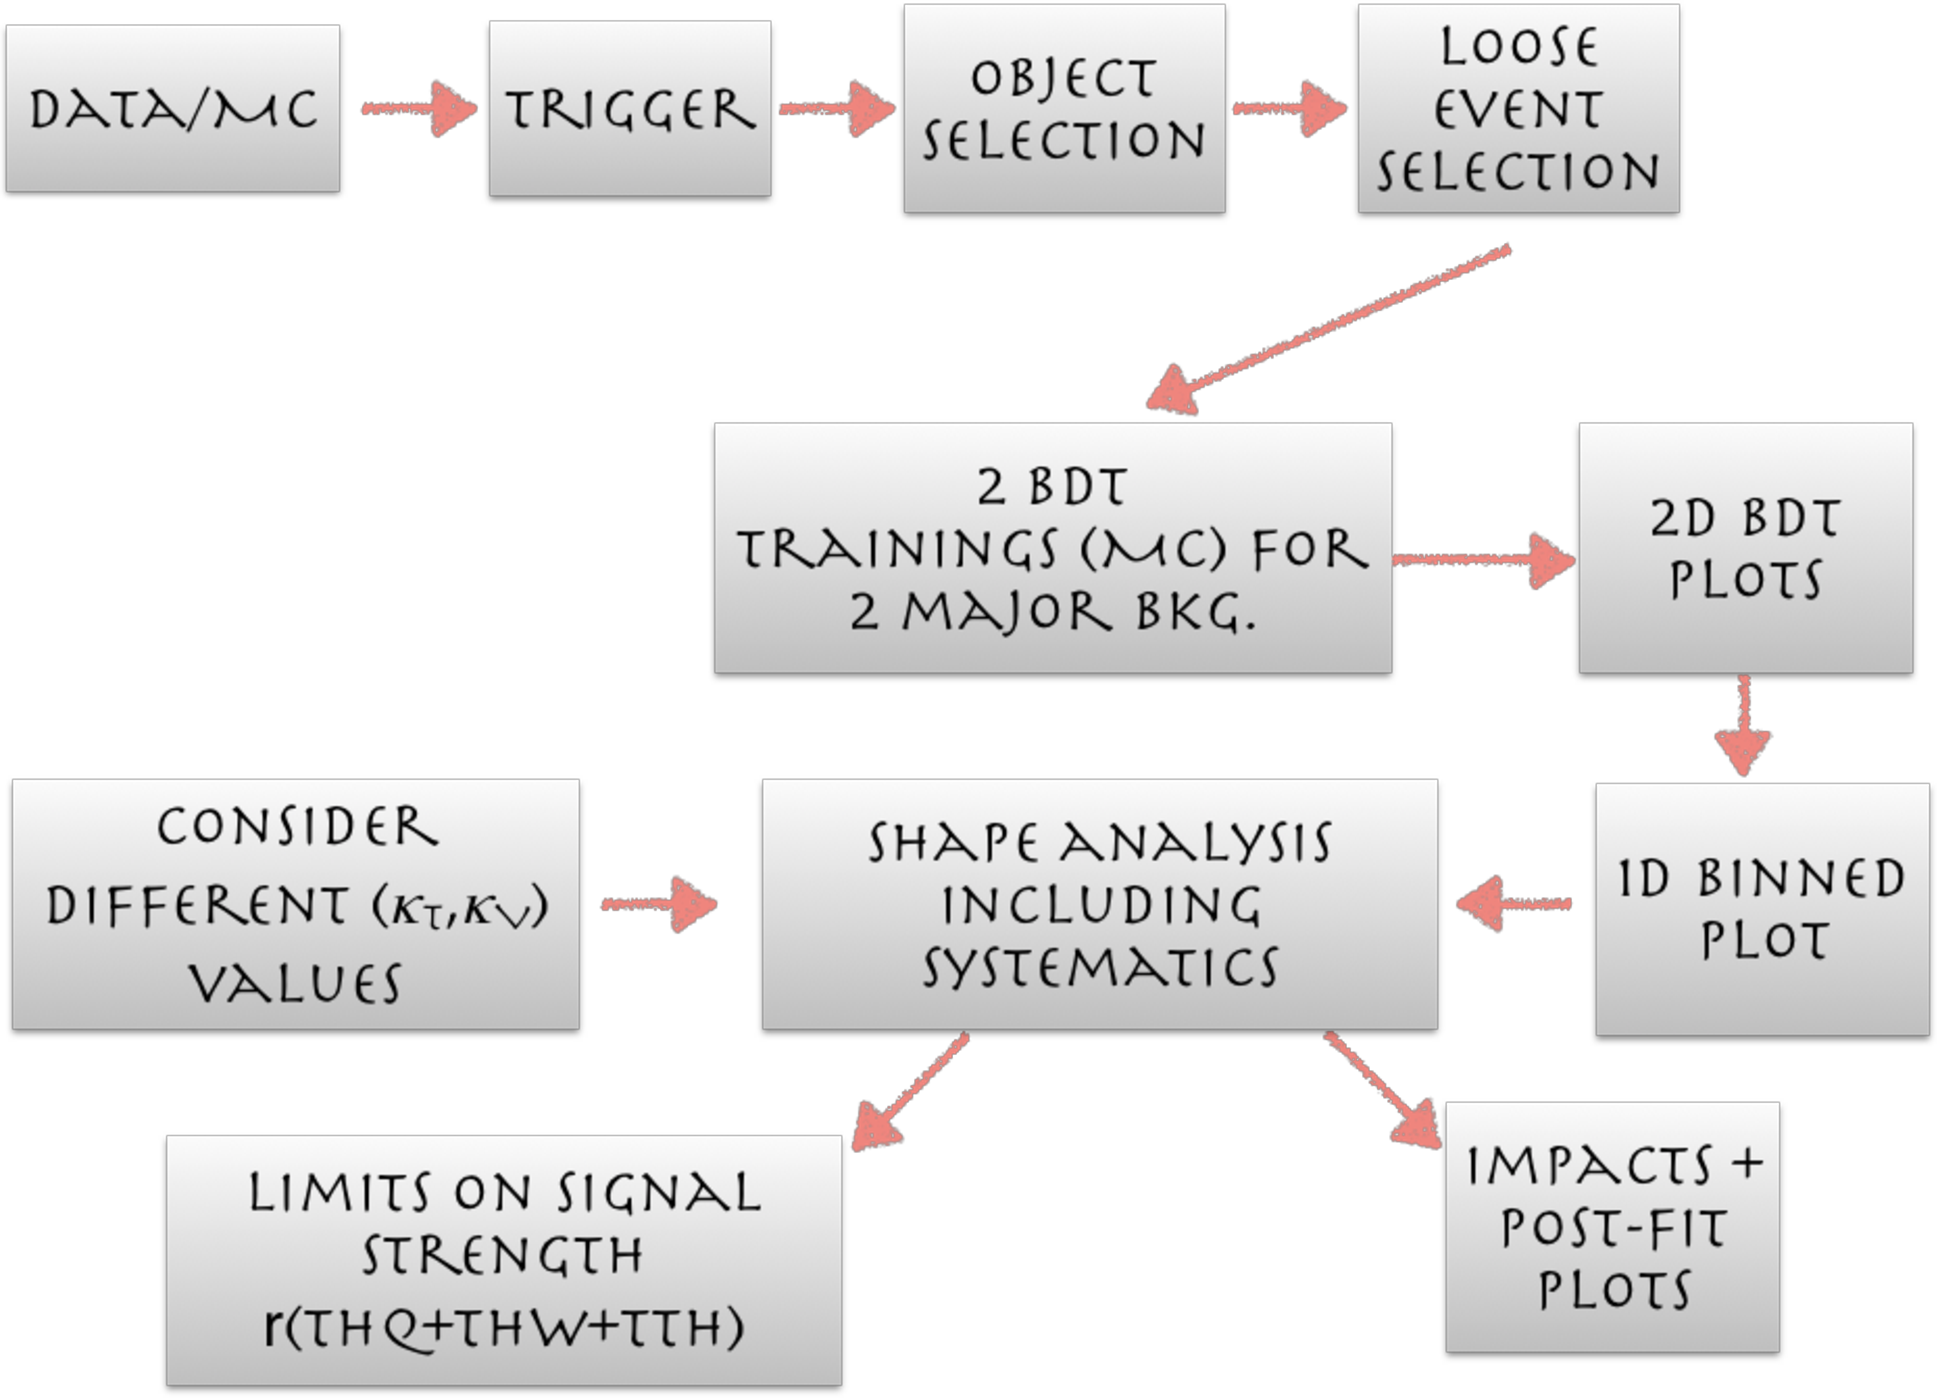
\includegraphics[width=\textwidth]{workflow}
\end{center}
\caption[Analysis strategy workflow]{A schematic overview of the analysis workflow. Based on sets of optimized physics object definitions and selection criteria, signal and background events in a data sample are discriminated. The discrimination is performed by a BDT, previously trained using MC samples of the dominant backgrounds, using discriminant variables based on the \bjet multiplicity, the activity in the forward region of the detector, and the kinematic properties of leptons. The $CL_s$ limits on the combined \ttH + \tH production cross section, as a function of the relative coupling strengths are calculated. }
\label{fig:workflow}
\end{figure}

The analysis is designed to efficiently identify and select prompt leptons from on-shell W and Z boson decays and to reject non-prompt leptons from $b$ quark decays and spurious lepton signatures from hadronic jets. Events are then selected in the $2lss$ and $3l$ channels, and are required to contain hadronic jets, some of which must be consistent with $b$ quark hadronization. Finally, the signal yield is extracted by simultaneously fitting the output of two dedicated multivariate discriminants, trained to separate the \tHq signal from the two dominant backgrounds which, as will be shown in Section \ref{sec:bg},  are \ttbar, \ttW and \ttZ processes. The fit result is then used to set an upper limit on the combined \ttH + \tH\ production cross section as a function of the relative coupling strengths of Higgs-top quark and Higgs-Vector boson. Figure \ref{fig:workflow} shows an schematic overview of the analysis strategy workflow. 

The analysis has been made public by CMS as a Physics Analysis Summary \cite{CMS_PAS_HIG_17-005} combining the result for the three lepton and two lepton same-sign channels; the content present in this chapter is based on that document and on References ~\cite{CMS_AN_2016-211, CMS_AN_2017-029} unless another reference is stated. Currently, an effort to turn the analysis into a paper combining the multilepton and $H \to b\bar{b}$ results is ongoing. 

%% dont forget to describe explicitely the analysis strategy here or later but do it

%---------------------------------tHq signature
\section{\tHq signature}\label{sec:thq_sign}

\begin{figure}[!h]
\begin{center}
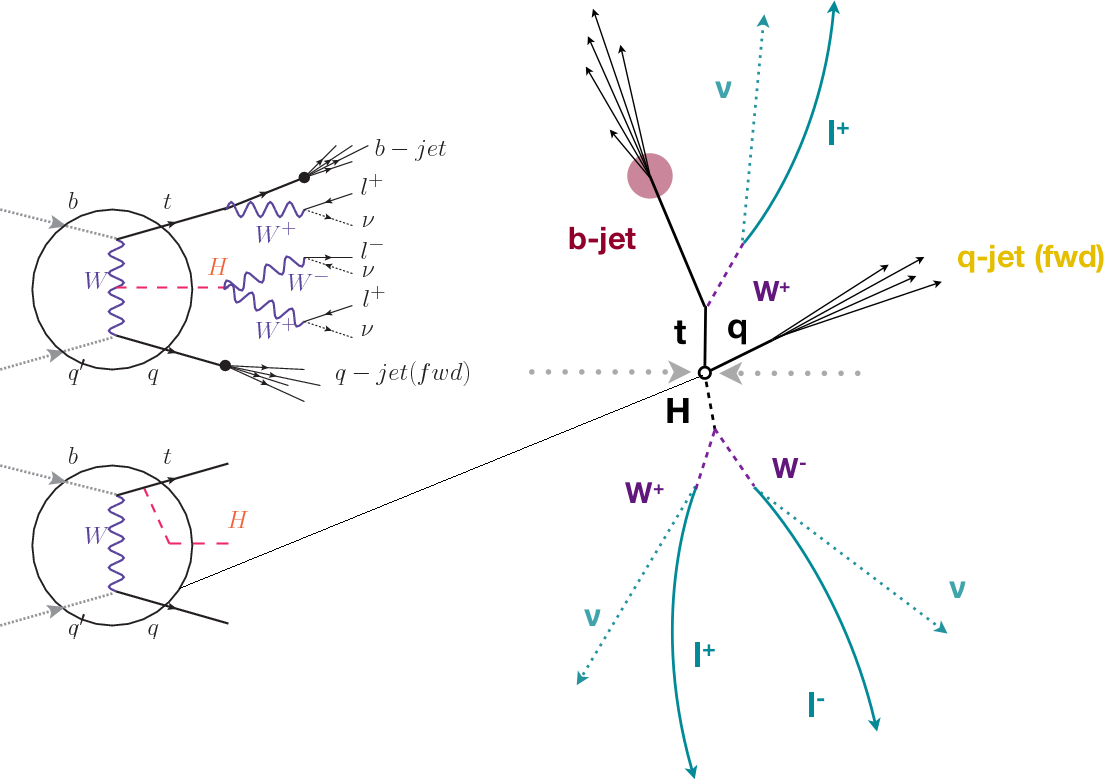
\includegraphics[width=\textwidth]{thq_sign}
\end{center}
\caption[\tHq event signature]{\tHq event signature. Left: Feynman diagram including the whole evolution up to the final state for the case of the Higgs boson emitted by the W boson (top); Feynman diagram for the case where the Higgs boson is emitted by the top quark. Right: Schematic view as it would be seen in the detector; the circle in the Feynman diagrams on the left corresponds to the circle in the center of the schematic view as indicated by the line connecting them. In the $2lss$ channel, one of the W bosons from the Higgs boson decays to two light-quark jets while in the $3l$ channel both W bosons decay to leptons.}
\label{fig:thq_sign}
\end{figure}

In order to select events of \tHq process, its features are translated into a set of selection rules; Figure \ref{fig:thq_sign} shows the Feynman diagram and a schematic view of the \tHq process from the \pp collision (at partonic level) to the final state configuration. A single top quark is produced accompanied by a light quark, denoted as q; this light quark is produced predominantly in the forward region of the detector. The Higgs boson can be either emitted by the exchanged W boson or directly by the singly produced top quark.

Due to their high masses/short lifetimes, the top quark and Higgs boson decay within the detector after their production. The Higgs boson is required to decay into a W boson pair. The top quark almost always decays into a bottom quark and a W boson, as encoded in the CMK matrix. The W bosons are required to decay leptonically either all the three in the $3l$ channel or the pair with equal electrical charge in the $2lss$ channel case; $\tau$ leptons are not reconstructed separately and only their leptonic decays into either electrons or muons are considered in this analysis.

In summary, the signal process is characterized by the final state with

\begin{itemize}
\item one light-flavored forward jet,
\item one central b-jet,
\item $2lss$ channel $\to$ two leptons of the same sign, two neutrinos and two, often soft, jets,
\item $3l$ channel $\to$ three leptons, three neutrinos and no central light-flavored jets.
\end{itemize}

The presence of neutrinos is inferred from the presence of MET.

Note that, $H \to ZZ$ and $H\to \tau\tau$ decays can produce the same final state as for $H\to WW$ decay; therefore, they are also include in the analysis but they are not separately reconstructed.

%---------------------------------bg processes

\section{Background processes}\label{sec:bg}

The background processes are those that can mimic the signal signature or at least can be reconstructed as signal as a result of certain circumstances. The backgrounds can be classified as

\begin{itemize}

\item irreducible backgrounds: where genuine prompt leptons are produced in on-shell W and Z boson decays; they can be reliably estimated directly from MC simulated events, using higher-order cross sections (NLO or NNLO or higher as available) or data control regions for the overall normalization.

\item reducible backgrounds: where at least one of the leptons is \ti{non-prompt}, \ie, produced within a hadronic jet; genuine leptons from heavy flavor decays and misreconstructed jets, also known as \ti{mis-ID leptons} are considered non-prompt leptons or or \ti{fake leptons} as well as electrons from photon conversions. These non-prompt leptons leave tracks and hits in the detection systems as would a prompt lepton, but evaluation of the correlation of those hits with nearby jets is a way of removing them. The misassignment of electron charge in processes like \ttbar or Drell-Yan, represents an additional source of background, but it is relevant only for the $2lss$ channel. Reducible backgrounds are not well predicted by simulation, hence, they are estimated using data-driven methods. 
\end{itemize}

The main sources of background events for \tHq process are the \ttbar process and \ttV $(V=W,Z,\gamma)$ processes. Figure \ref{fig:ttbar_sign} shows the signature for \ttbar and \ttW processes.     

\begin{figure}[!htb]
\centering
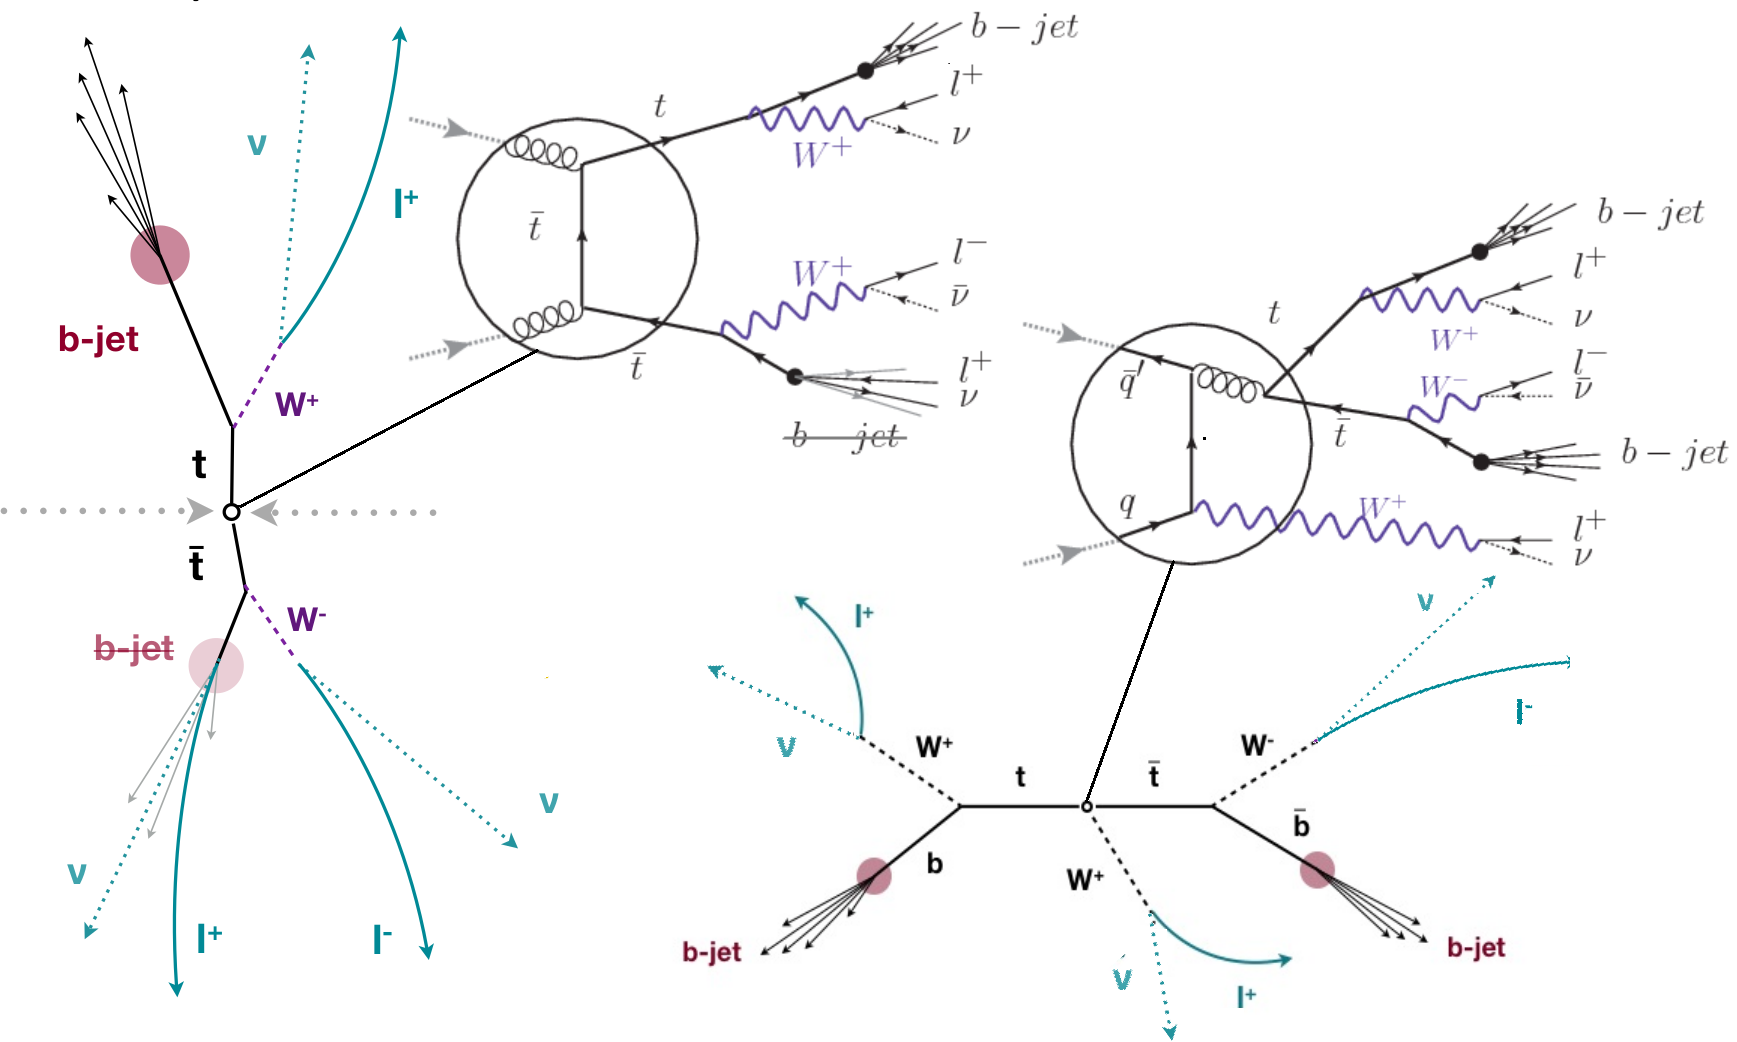
\includegraphics[width=\textwidth]{ttbar_signature}
\caption[\ttbar and \ttW events signature]{\ttbar(left) and \ttW (right) events signature as they would be seen in the detector; the Feynman diagrams including the whole evolution up to the final state are also shown. The \ttbar process signature is very similar to that of the signal process with one \bjet misidentified as a lepton (fake lepton indicated with the \bjet tag struck through) and no forward activity. The \ttW\ process presents a higher b-jet multiplicity compared to the signal process, a prompt lepton and no forward activity.}
\label{fig:ttbar_sign}
\end{figure}

The largest contribution to irreducible backgrounds comes from \ttW and \ttZ\ processes for which the number of ($b-$)jets (($b-$)jet multiplicity) is higher than that of the signal events, while for other contributing background events,  \WZ, $ZZ$, and rare SM processes like $W^\pm W^\pm qq$, $\ttbar\ttbar$, $tZq$, $tZW$, $WWW$, $WWZ$, $WZZ$, $ZZZ$, the ($b-$)jet multiplicity is lower compared to that of the signal events. None of the irreducible backgrounds present activity in the forward region of the detector.

On the side of the reducible backgrounds, the largest contribution comes from the \ttbar events which have a very similar signature to the signal events but does no present activity in the forward region of the detector either; A particular feature of the \ttbar events is their charge-symmetry, which is different from the characteristics of signal events.
%______________________ Samples  ______________________
\section{Data and MC Samples} \label{secc:samples}

\subsection{ Full 2016 data set}

The data set used in this analysis was collected by the CMS experiment during 2016, while running at $\sqrt{s}=13$ TeV, and corresponds to a total integrated luminosity of 35.9 \fbinv. Only periods when the CMS magnet was on were considered when selecting the data samples; that corresponds to the \verb|23Sep2016 (Run B to G)| and \verb|PromptReco (Run H)| versions of the datasets.

Multilepton final states with either two same-sign leptons or three leptons target the case where the Higgs boson decays to a pair of W bosons, $\tau$ leptons, or Z bosons, and where the top quark decays leptonically, hence, the \verb|SingleElectron|, \verb|SingleMuon|, \verb|DoubleEG|, \verb|MuonEG|, \verb|DoubleMuon| dataset (see Table \ref{tab:dataset}) compose the full dataset. The selected sample has contributions from $H\to WW (\sim 75\%)$, $ZZ (\sim 25\%)$, $\tau\tau (\sim 5\%)$.

The quality of the data sets is evaluated by considering any observation reported from the CMS control room where the status of each detection system is monitored; thus, if ,for instance, an unusual behavior in the solenoid is reported, the data sets produced with the data taken at that are accordingly flagged. In fact, information about alignment, calibration, luminosity, detectors status, among others is used to qualify the data sets. Part of the qualification is make online (during the data taking) while further qualifications are preformed offline when the data are stored and processed at the Tier-0 and Tier-1 data processing centers.

Usually, during the offline qualification, experts from the sub detection systems teams check the data quality based on the performance of their subsystems by looking at histograms specifically tailored to catch relevant problems; then, a single boolean flag is assigned to describe the final quality result. Data are defined as \ti{good for physics analysis} if all subdetectors, trigger and physics object (tracking, electron, muon, gamma, jet and MET) show the expected performance. A complete description of data certification strategy is documented in Reference \cite{dqm}. 

Qualification results include the information about the luminosity delivered by LHC, the luminosity recorded by CMS and the luminosity certified as Good for physics analysis. In particular, the \ti{luminosity section} which is a sub-section of a run during which the instantaneous luminosity is unchanging; is used as the unit of accounting for integrated luminosity, hence, production data files contain one or many whole luminosity sections. The certified luminosity sections are listed in a JSON formatted file\footnote{JSON stands for JavaScript Object Notation} known as the \ti{golden JSON file} defined by the CMS experiment \cite{json}.

\subsection{Triggers}

The events considered are those online-reconstructed events triggered by one, two, or three leptons. Single-lepton triggers are included in order to boost the acceptance of events where the \pt of the sub-leading lepton falls below the threshold of the double-lepton triggers. The trigger efficiency is increased by including double-lepton triggers in the $3l$ category, and single-lepton triggers in all categories; it is possible given the logical ``or'' of the trigger decisions of all the individual triggers in a given category. Table ~\ref{tab:triggers} shows the lowest-threshold non-prescaled triggers present in the HLT menus for both Monte Carlo and data in 2016.

\subsubsection*{Trigger efficiency scale factors}

\begin{figure}[htp]
\centering
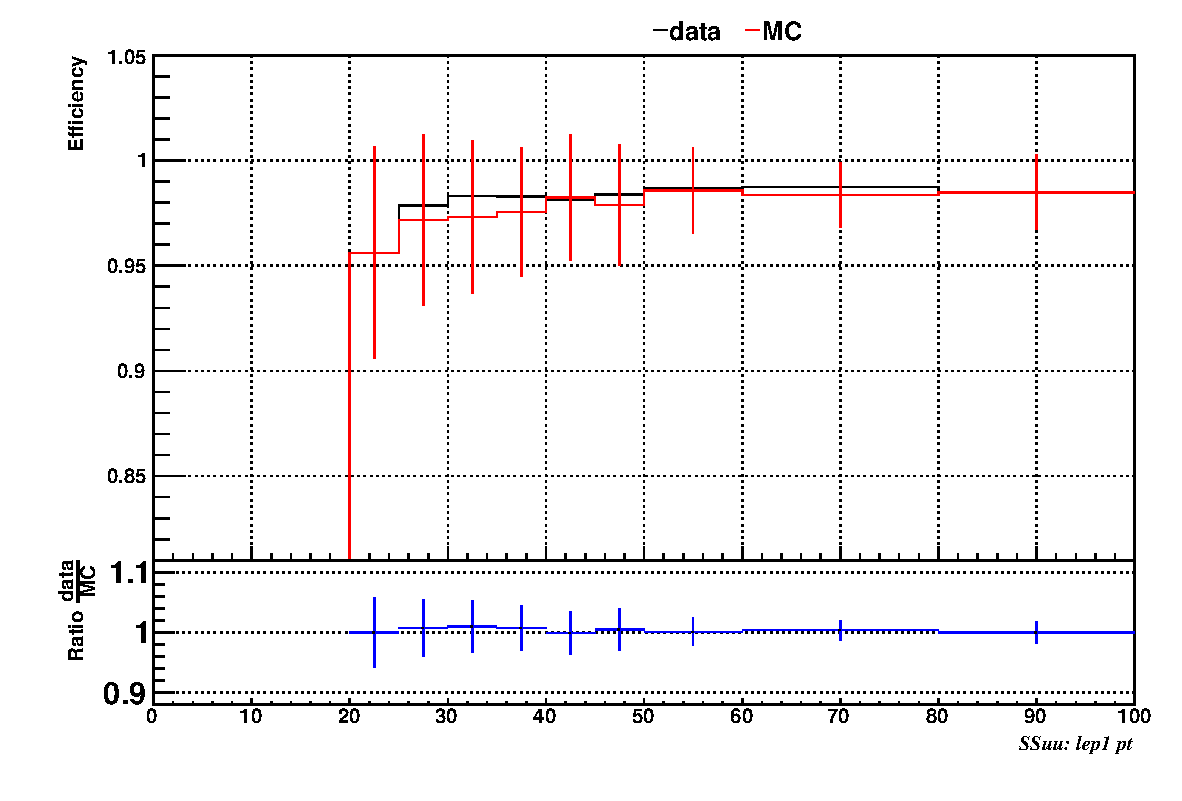
\includegraphics[width=0.49\textwidth]{plots_trigger/1D_eff_lep1_pt_uu_ARCv2_change_3l_pt_ranges.pdf}
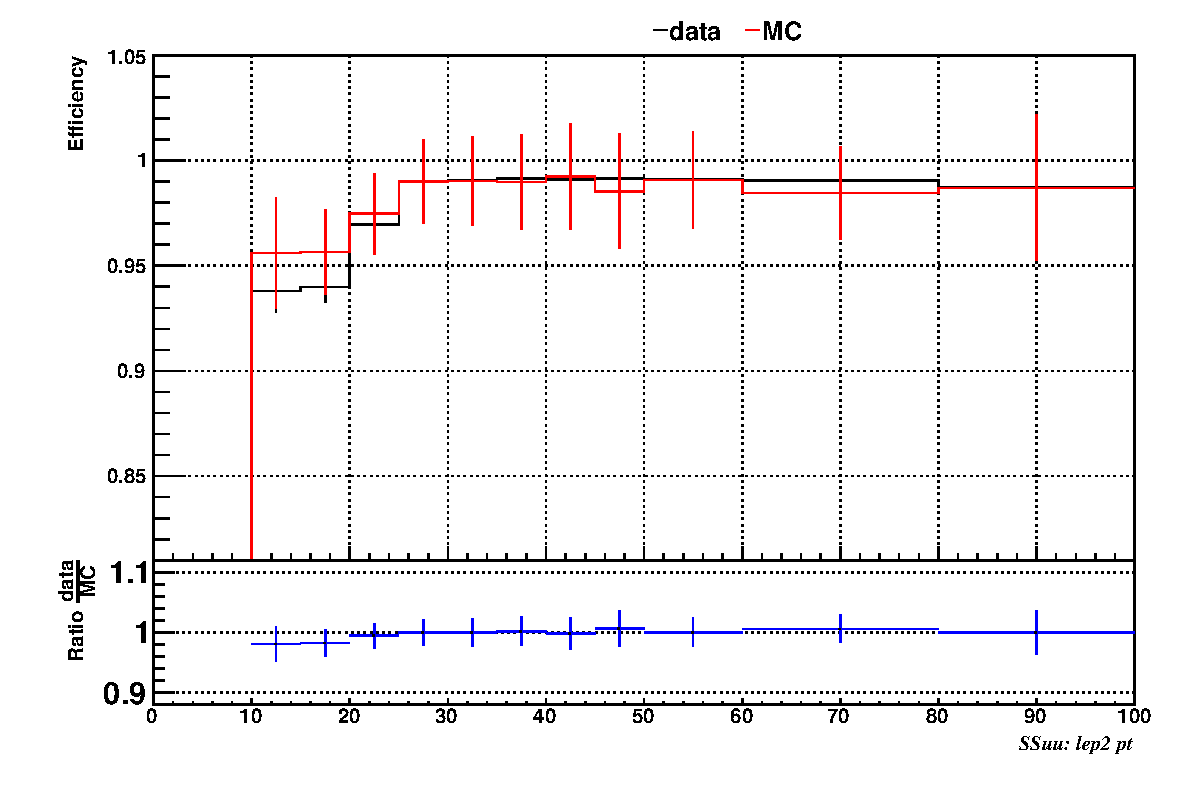
\includegraphics[width=0.49\textwidth]{plots_trigger/1D_eff_lep2_pt_uu_ARCv2_change_3l_pt_ranges.pdf} \\
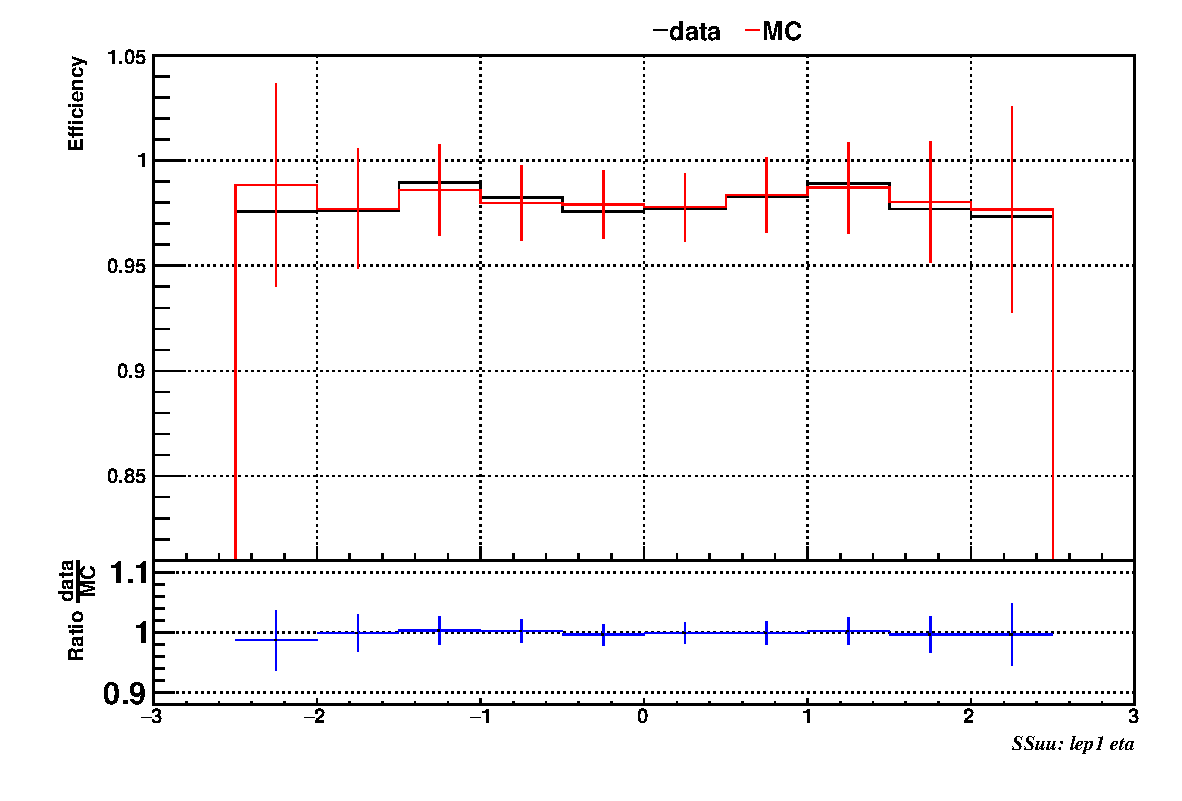
\includegraphics[width=0.49\textwidth]{plots_trigger/1D_eff_lep1_eta_uu_ARCv2_change_3l_pt_ranges.pdf}
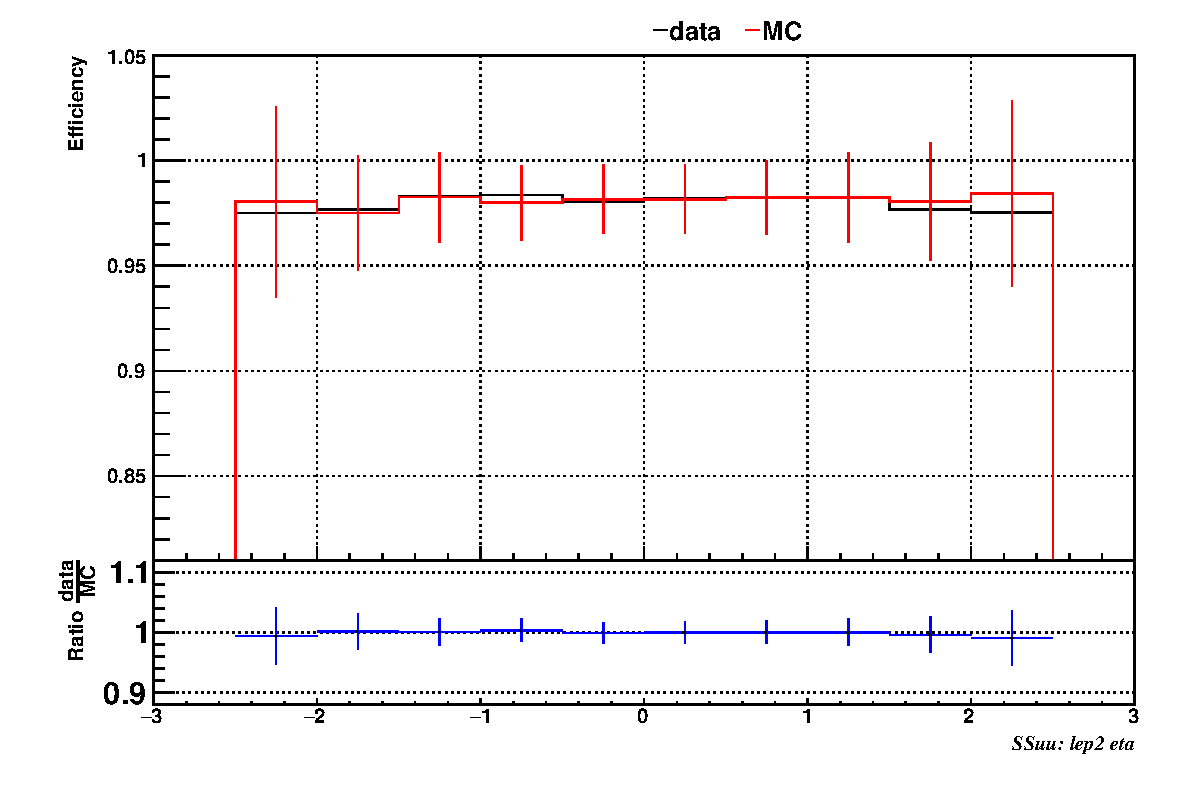
\includegraphics[width=0.49\textwidth]{plots_trigger/1D_eff_lep2_eta_uu_ARCv2_change_3l_pt_ranges.pdf}
\caption[Trigger efficiency for the same-sign $\mu\mu$ category]{Comparison between data an MC trigger efficiencies in the same-sign $\mu\mu$ category, as a function of the \pt (top) and \etac (bottom) of the leading lepton (left) and the sub-leading lepton (right). The lower panes show the data/MC ratio. \cite{CMS_AN_2017-029}.}
\label{fig:trigeffsmumu}
\end{figure}

\begin{figure}[htp]
\centering
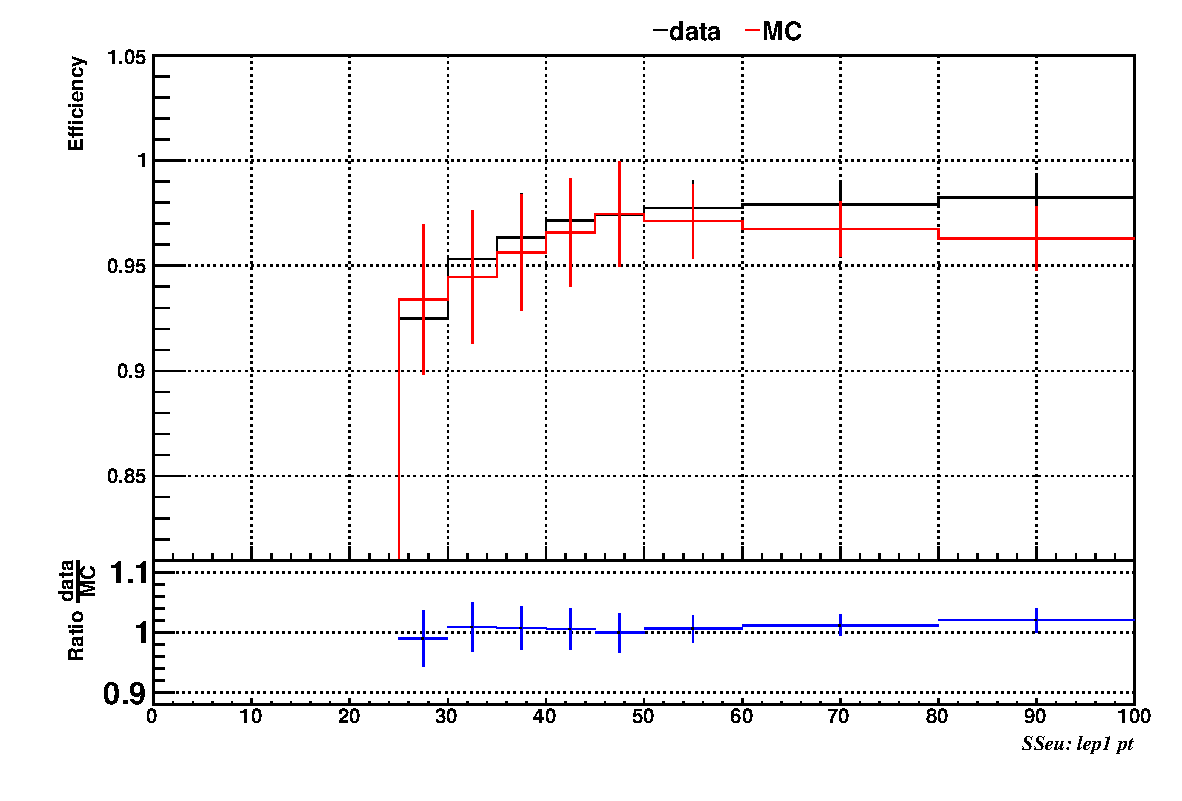
\includegraphics[width=0.49\textwidth]{plots_trigger/1D_eff_lep1_pt_eu_ARCv2_change_3l_pt_ranges.pdf}
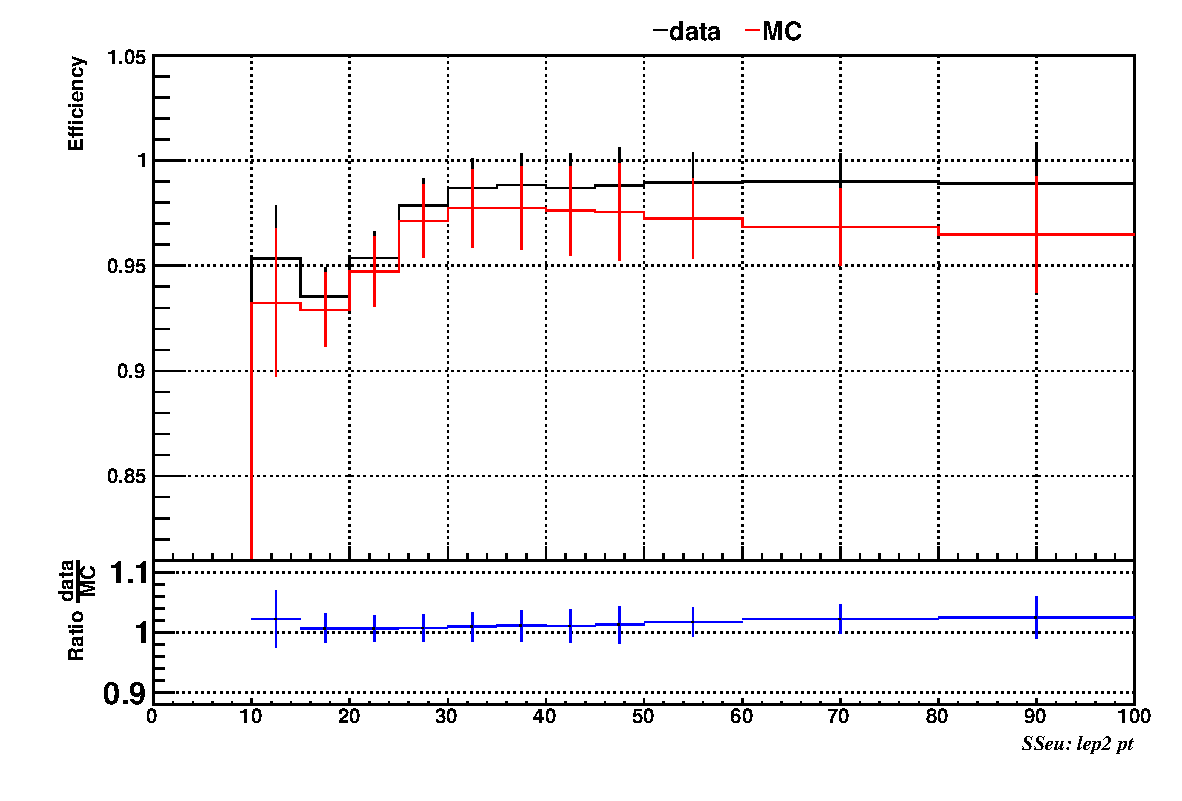
\includegraphics[width=0.49\textwidth]{plots_trigger/1D_eff_lep2_pt_eu_ARCv2_change_3l_pt_ranges.pdf} \\
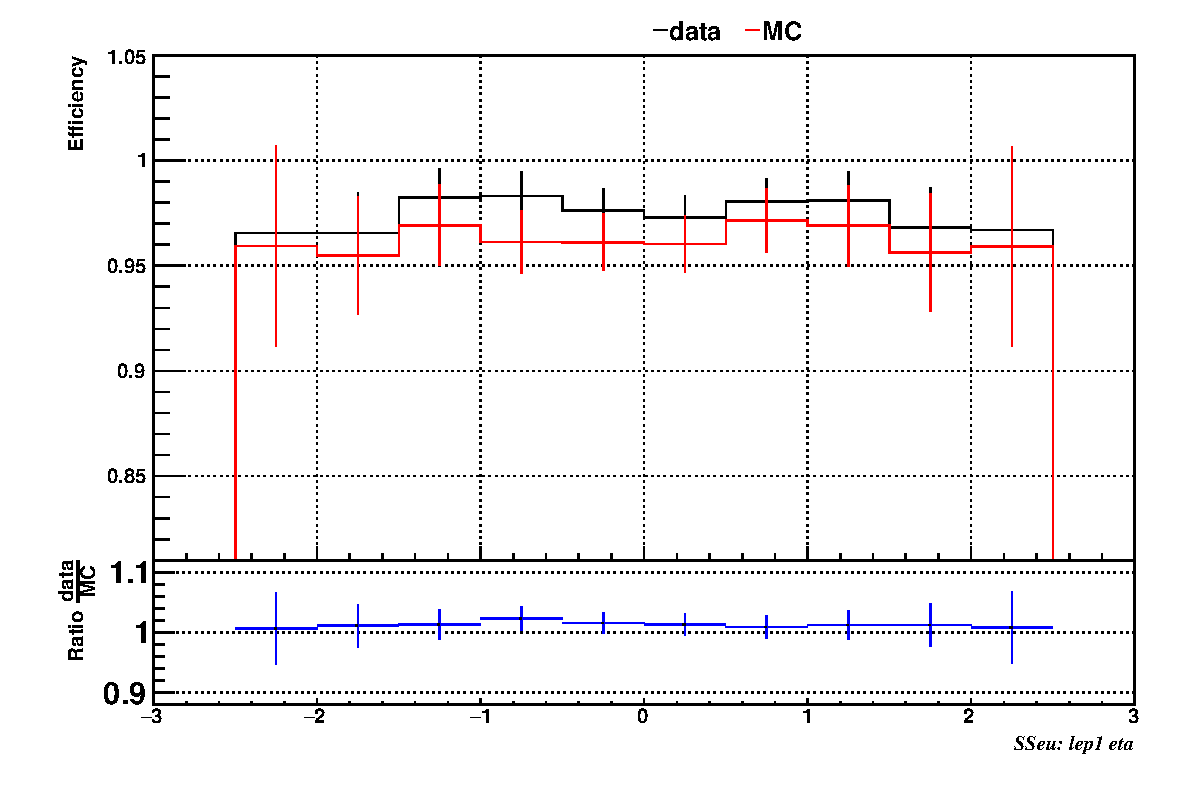
\includegraphics[width=0.49\textwidth]{plots_trigger/1D_eff_lep1_eta_eu_ARCv2_change_3l_pt_ranges.pdf}
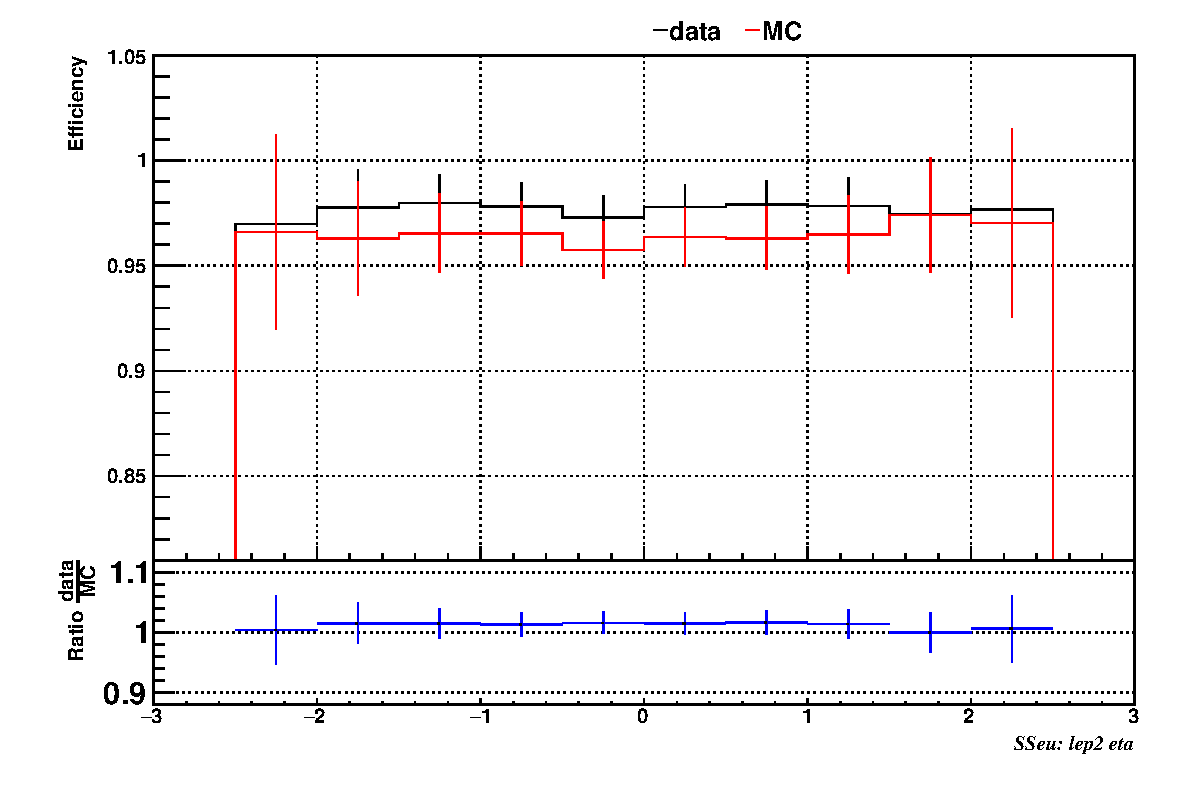
\includegraphics[width=0.49\textwidth]{plots_trigger/1D_eff_lep2_eta_eu_ARCv2_change_3l_pt_ranges.pdf}
\caption[Trigger efficiency for the $e\mu$ category]{Comparison between data an MC trigger efficiencies in the same-sign $e\mu$ category as a function of the \pt (top) and \etac (bottom) of the leading lepton (left) and the sub-leading lepton (right). The lower panes show the data/MC ratio. \cite{CMS_AN_2017-029}.}
\label{fig:trigeffsemu}
\end{figure}

%\begin{figure}[htp]
%\centering
%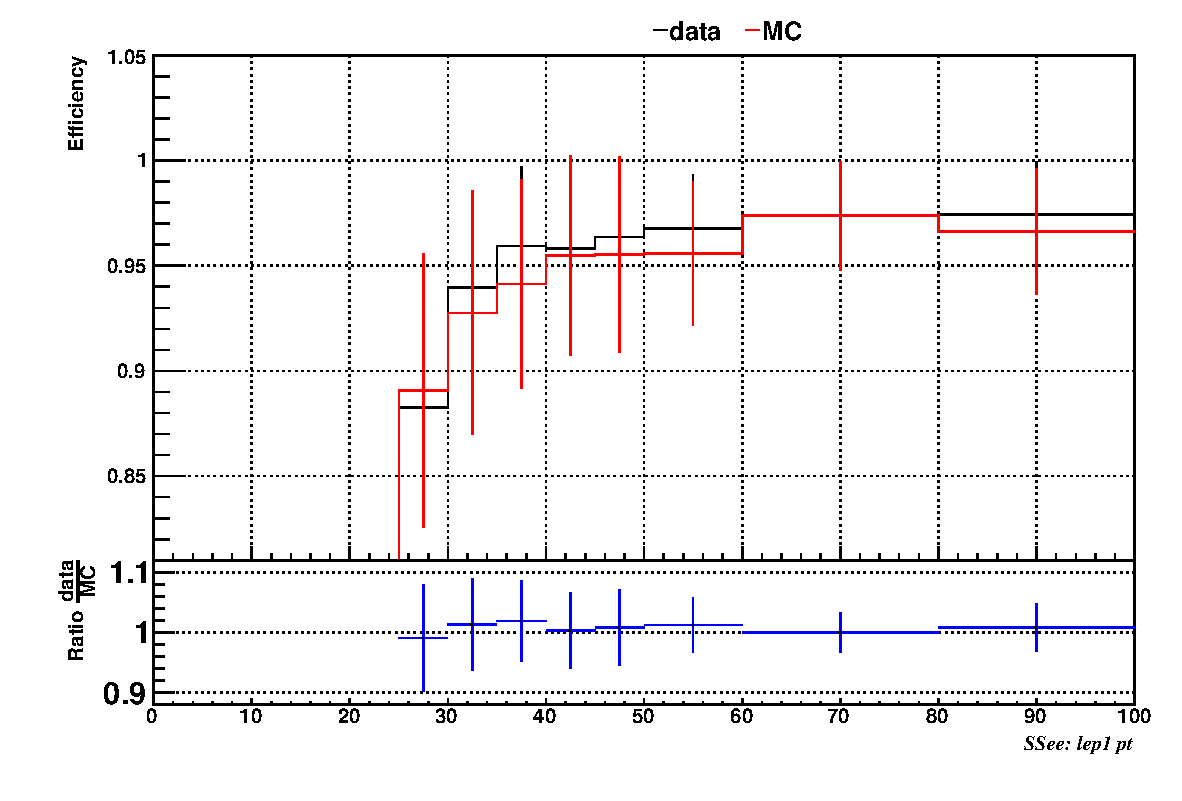
\includegraphics[width=0.49\textwidth]{plots_trigger/1D_eff_lep1_pt_ee_ARCv2_change_3l_pt_ranges.pdf}
%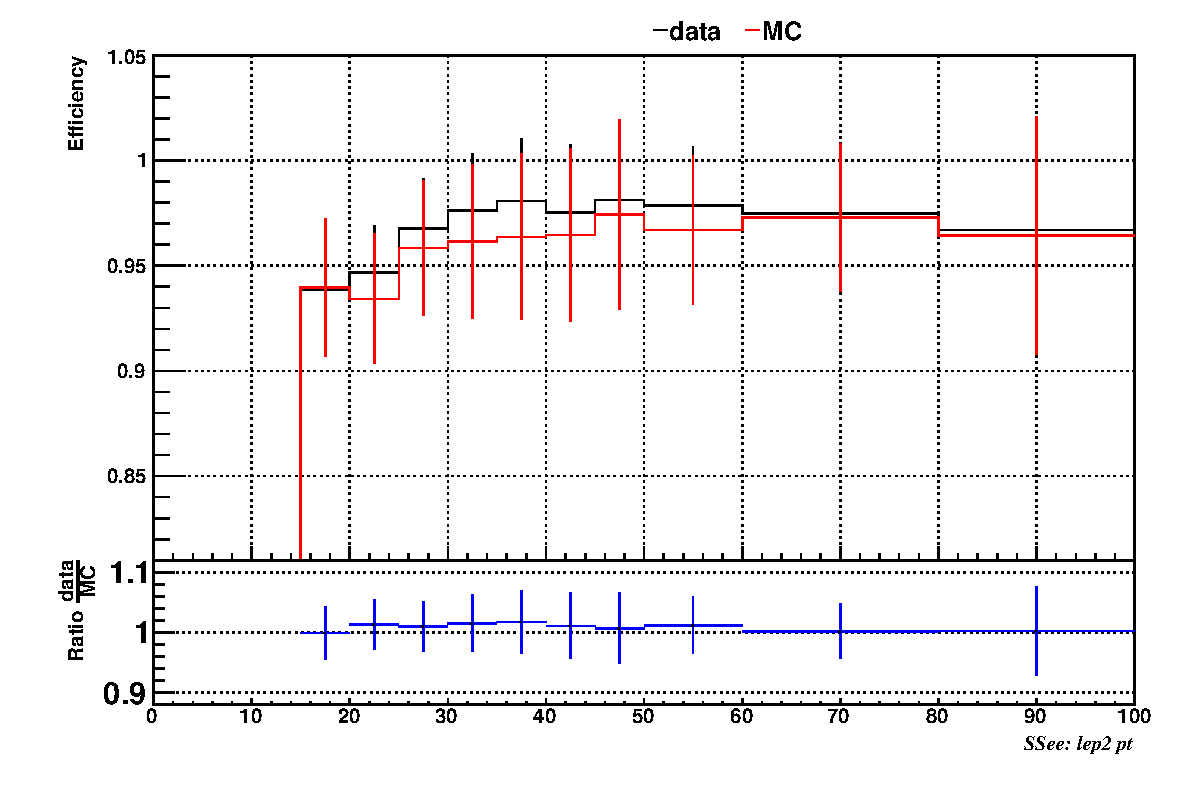
\includegraphics[width=0.49\textwidth]{plots_trigger/1D_eff_lep2_pt_ee_ARCv2_change_3l_pt_ranges.pdf} \\
%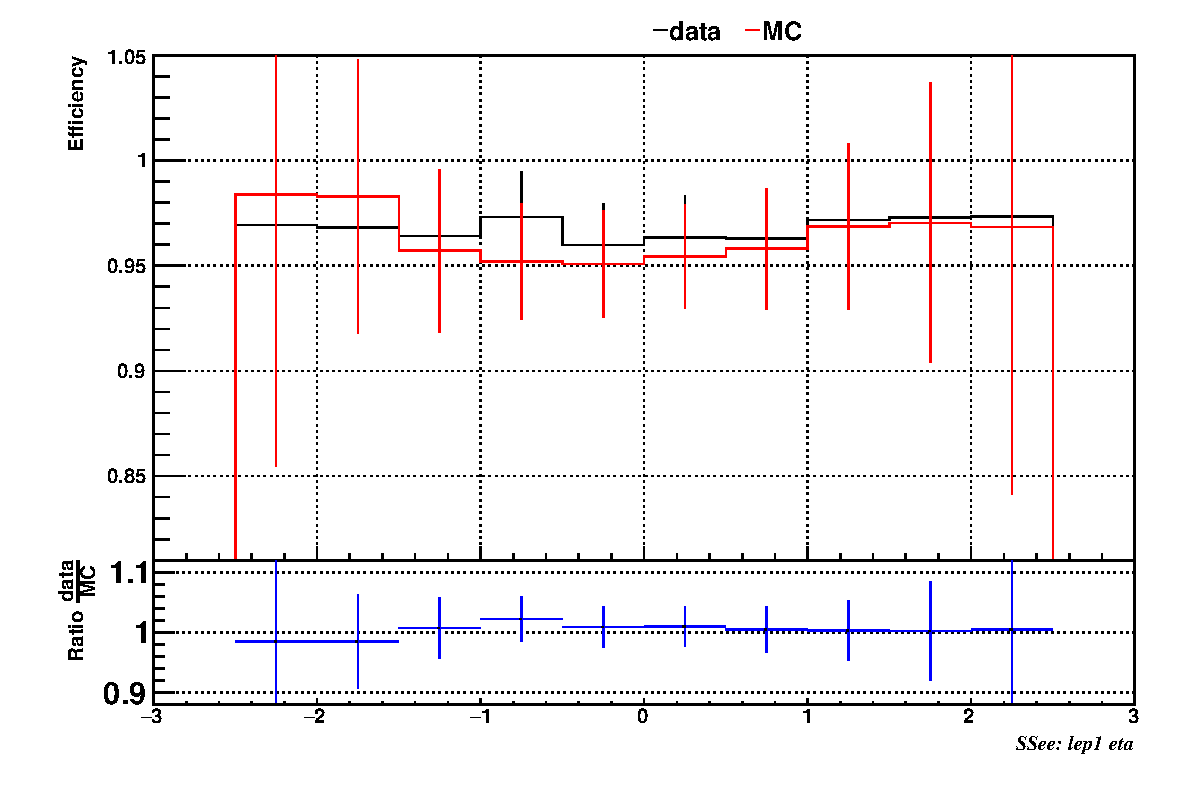
\includegraphics[width=0.49\textwidth]{plots_trigger/1D_eff_lep1_eta_ee_ARCv2_change_3l_pt_ranges.pdf}
%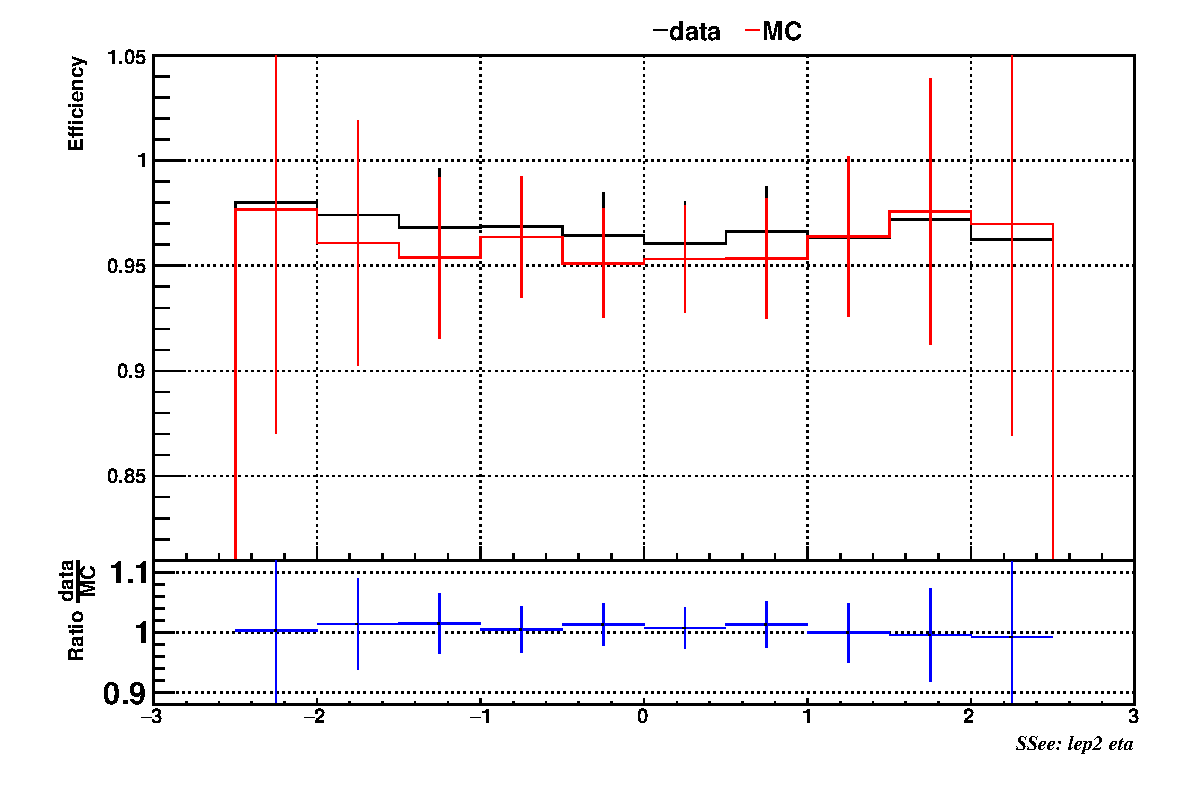
\includegraphics[width=0.49\textwidth]{plots_trigger/1D_eff_lep2_eta_ee_ARCv2_change_3l_pt_ranges.pdf}
%\caption[Trigger efficiency for the $ee$ category]{Comparison between data an MC trigger efficiencies in the same-sign $e\mu$ category ($1^{rs}$ and $2^{nd}$ rows) and same-sign $ee$ category ($3^{rd}$ and $4^{th}$ rows), as as a function of the \pt and $\eta$ of the leading lepton (left) and the sub-leading lepton (right) \cite{CMS_AN_2017-029}.}
%\label{fig:trigeffsee}
%\end{figure}

\begin{figure}[htp]
\centering
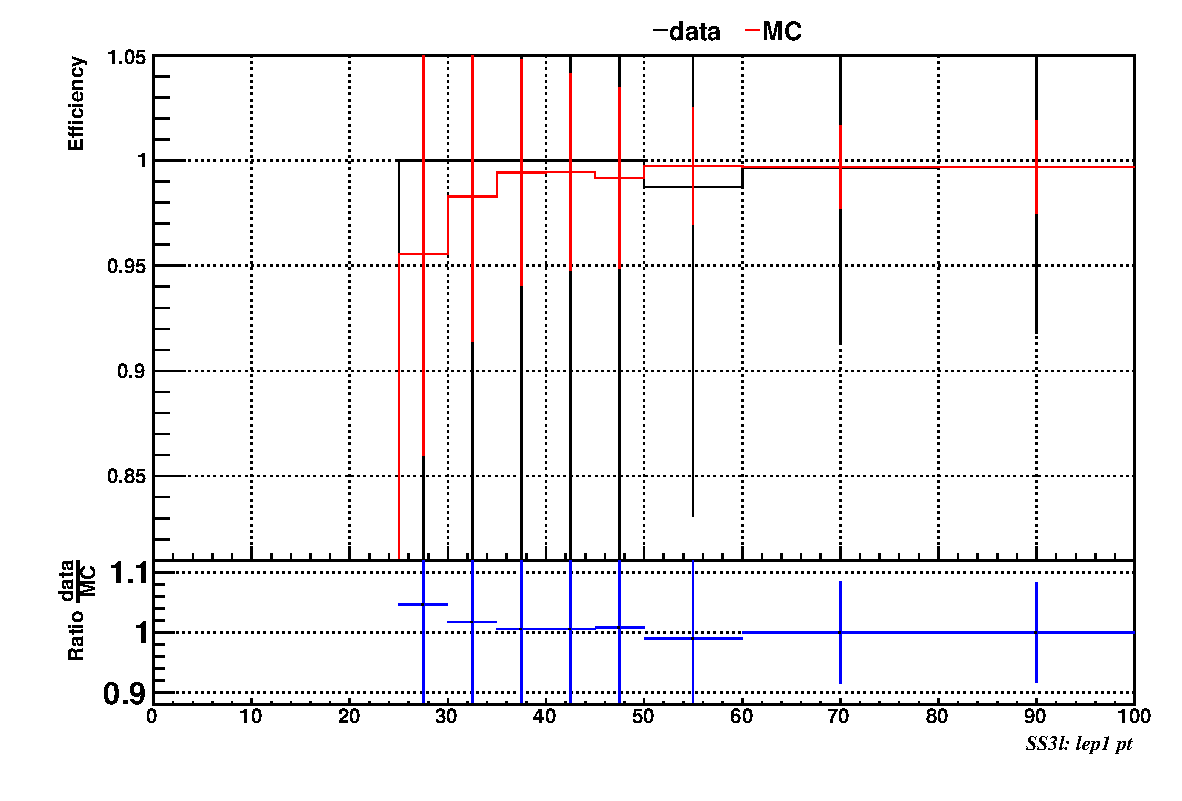
\includegraphics[width=0.49\textwidth]{plots_trigger/1D_eff_lep1_pt_3l_ARCv2_change_3l_pt_ranges.pdf}
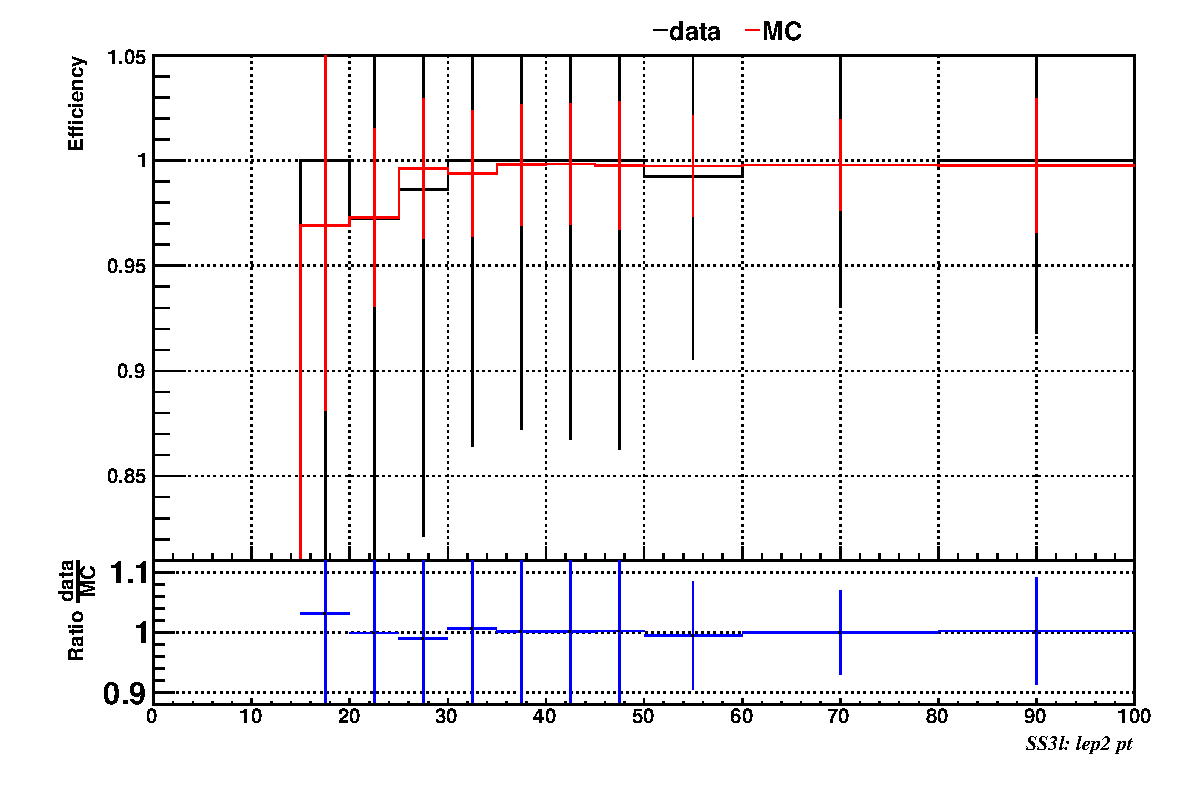
\includegraphics[width=0.49\textwidth]{plots_trigger/1D_eff_lep2_pt_3l_ARCv2_change_3l_pt_ranges.pdf} \\
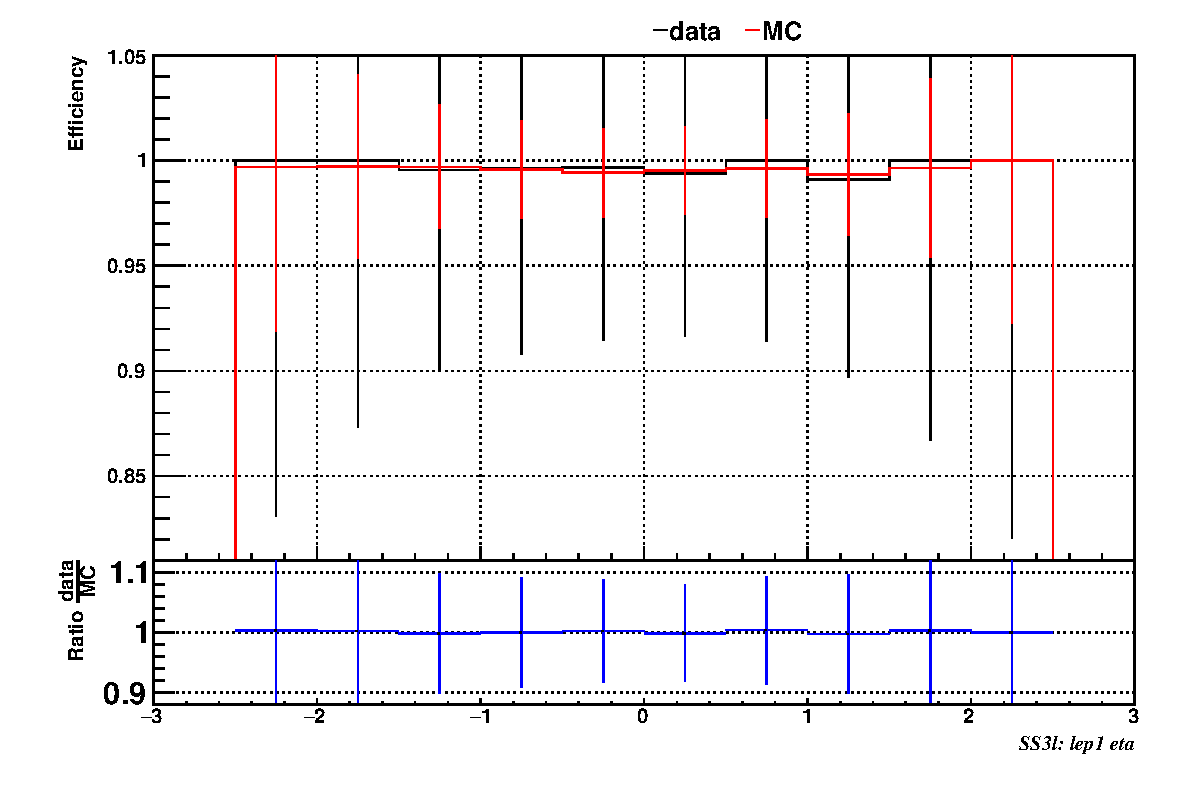
\includegraphics[width=0.49\textwidth]{plots_trigger/1D_eff_lep1_eta_3l_ARCv2_change_3l_pt_ranges.pdf}
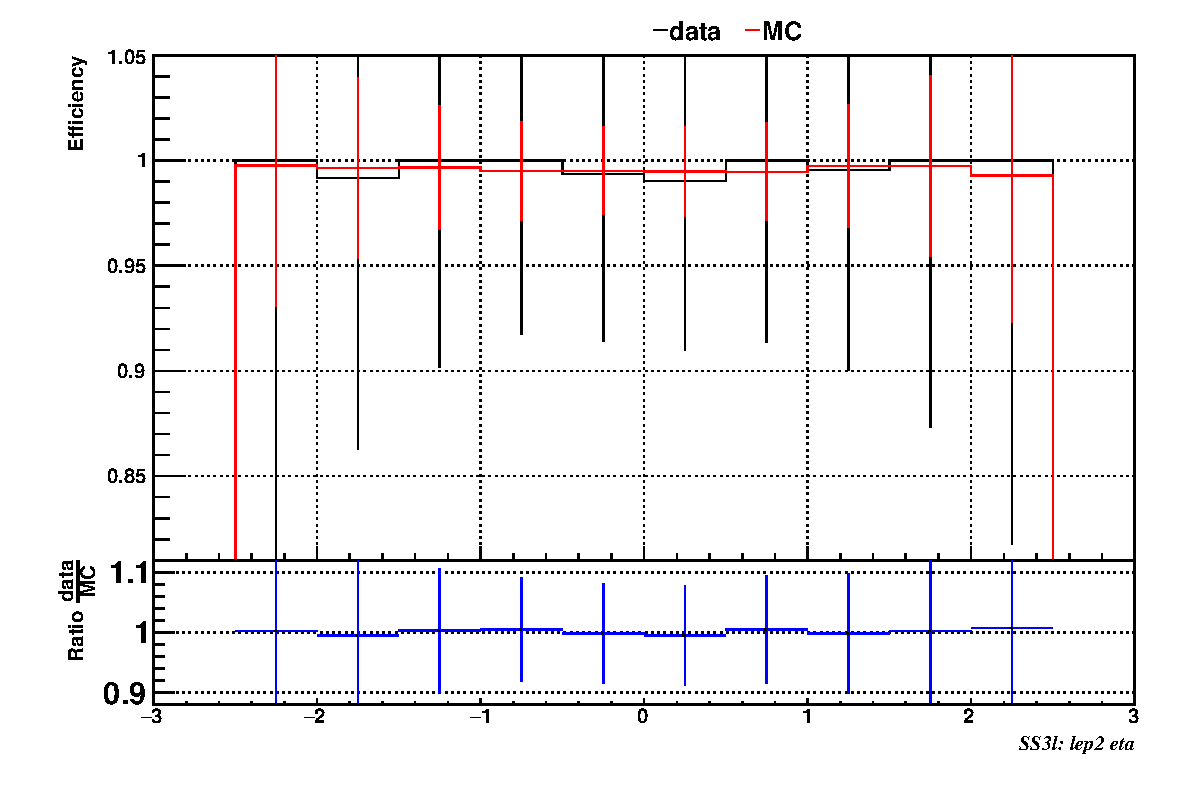
\includegraphics[width=0.49\textwidth]{plots_trigger/1D_eff_lep2_eta_3l_ARCv2_change_3l_pt_ranges.pdf}
\caption[Trigger efficiency for the $3l$ category]{Comparison between data an MC trigger efficiencies in the $3l$ category, as a function of the \pt (top) and \etac (bottom) of the leading lepton (left) and the sub-leading lepton (right). The lower panes show the data/MC ratio. \cite{CMS_AN_2017-029}.}
\label{fig:trigeffs3l}
\end{figure}

Trigger efficiency describes the probability of events to pass the trigger requirements. It is measured in simulated events using generator information given that there is no trigger bias with the MC sample. Measuring the trigger efficiency in data requires a more elaborate procedure; first, select a set of events collected by a trigger that is uncorrelated with the lepton triggers such that the selected events form an unbiased sample. In this analysis, that uncorrelated trigger is a MET trigger. Second step is looking for candidate events with exactly two leptons (exactly three leptons for the $3l$ channel). Finally,  measure the efficiency for the candidate events to pass the logical ``or'' of triggers being considered in a given event category as defined in Table ~\ref{tab:triggers}.

Comparisons between the data and MC efficiencies for each category, shown in Figures~\ref{fig:trigeffsmumu}, \ref{fig:trigeffsemu}, and \ref{fig:trigeffs3l}, reveal that they are in good agreement; the difference is corrected by applying scale factors derived from the ratio between both efficiencies.

Applied flat scale factors in each category are shown in Table ~\ref{tab:trigSFs}; they have been inherited from Reference \cite{CMS_AN_2017-029}. 

\begin{table}
\centering
\begin{tabular}{ll}
Category & Scale Factor \\\hline
    ee   & $1.01 \pm 0.02$ \\
e$\mu$   & $1.01 \pm 0.01$ \\
$\mu\mu$ & $1.00 \pm 0.01$ \\
3l       & $1.00 \pm 0.03$ \\\hline
\end{tabular}
\caption[Trigger efficiency scale factors and associated uncertainties.]{Trigger efficiency scale factors and associated uncertainties, shown here rounded to the nearest percent.}
\label{tab:trigSFs}
\end{table}

\subsection{MC samples}

Current event generators allow the adjustment of the kinematics of the generated events, based on an event-wise reweighting; in this way, several generation parameter phase spaces can be explored according to the experimental interests. The signal samples used in this analysis were generated in such a way that not only the ${\Ct=-1}$ case, but an extended range of \Ct and \CV values may be investigated.

\begin{figure}[htp]
\centering
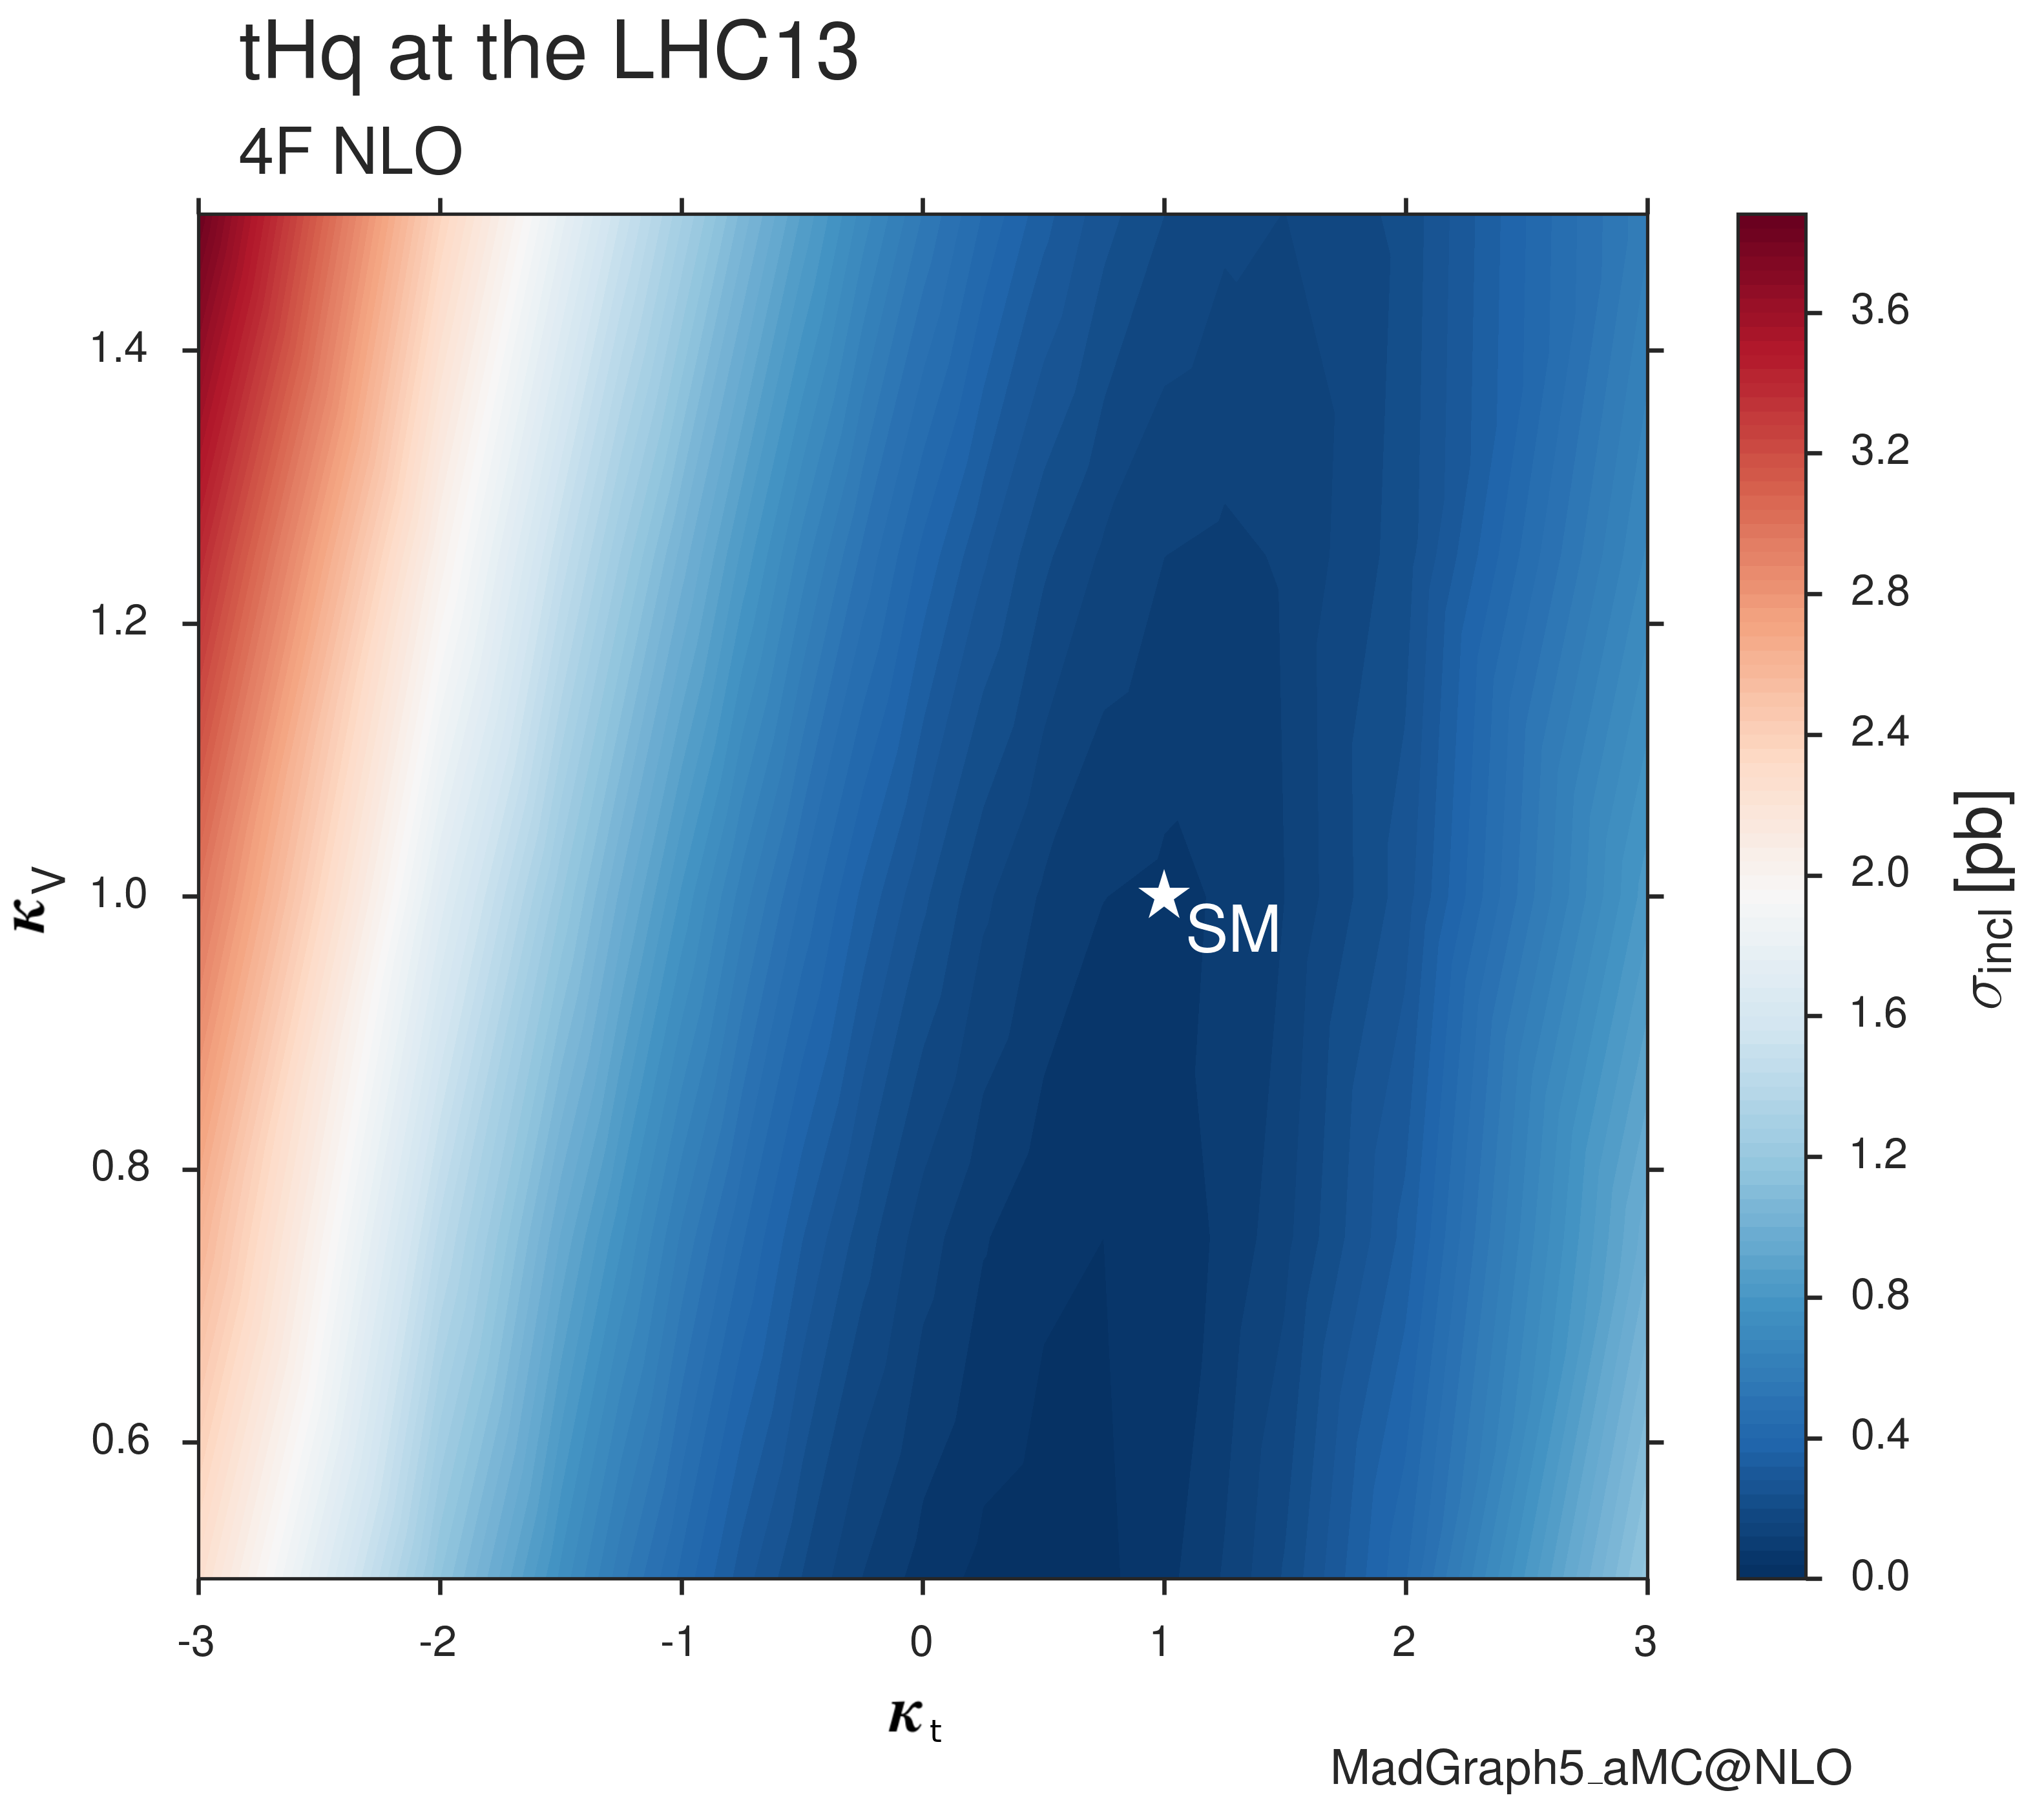
\includegraphics[width=0.49\textwidth]{tHQ_xsec_cfcv}
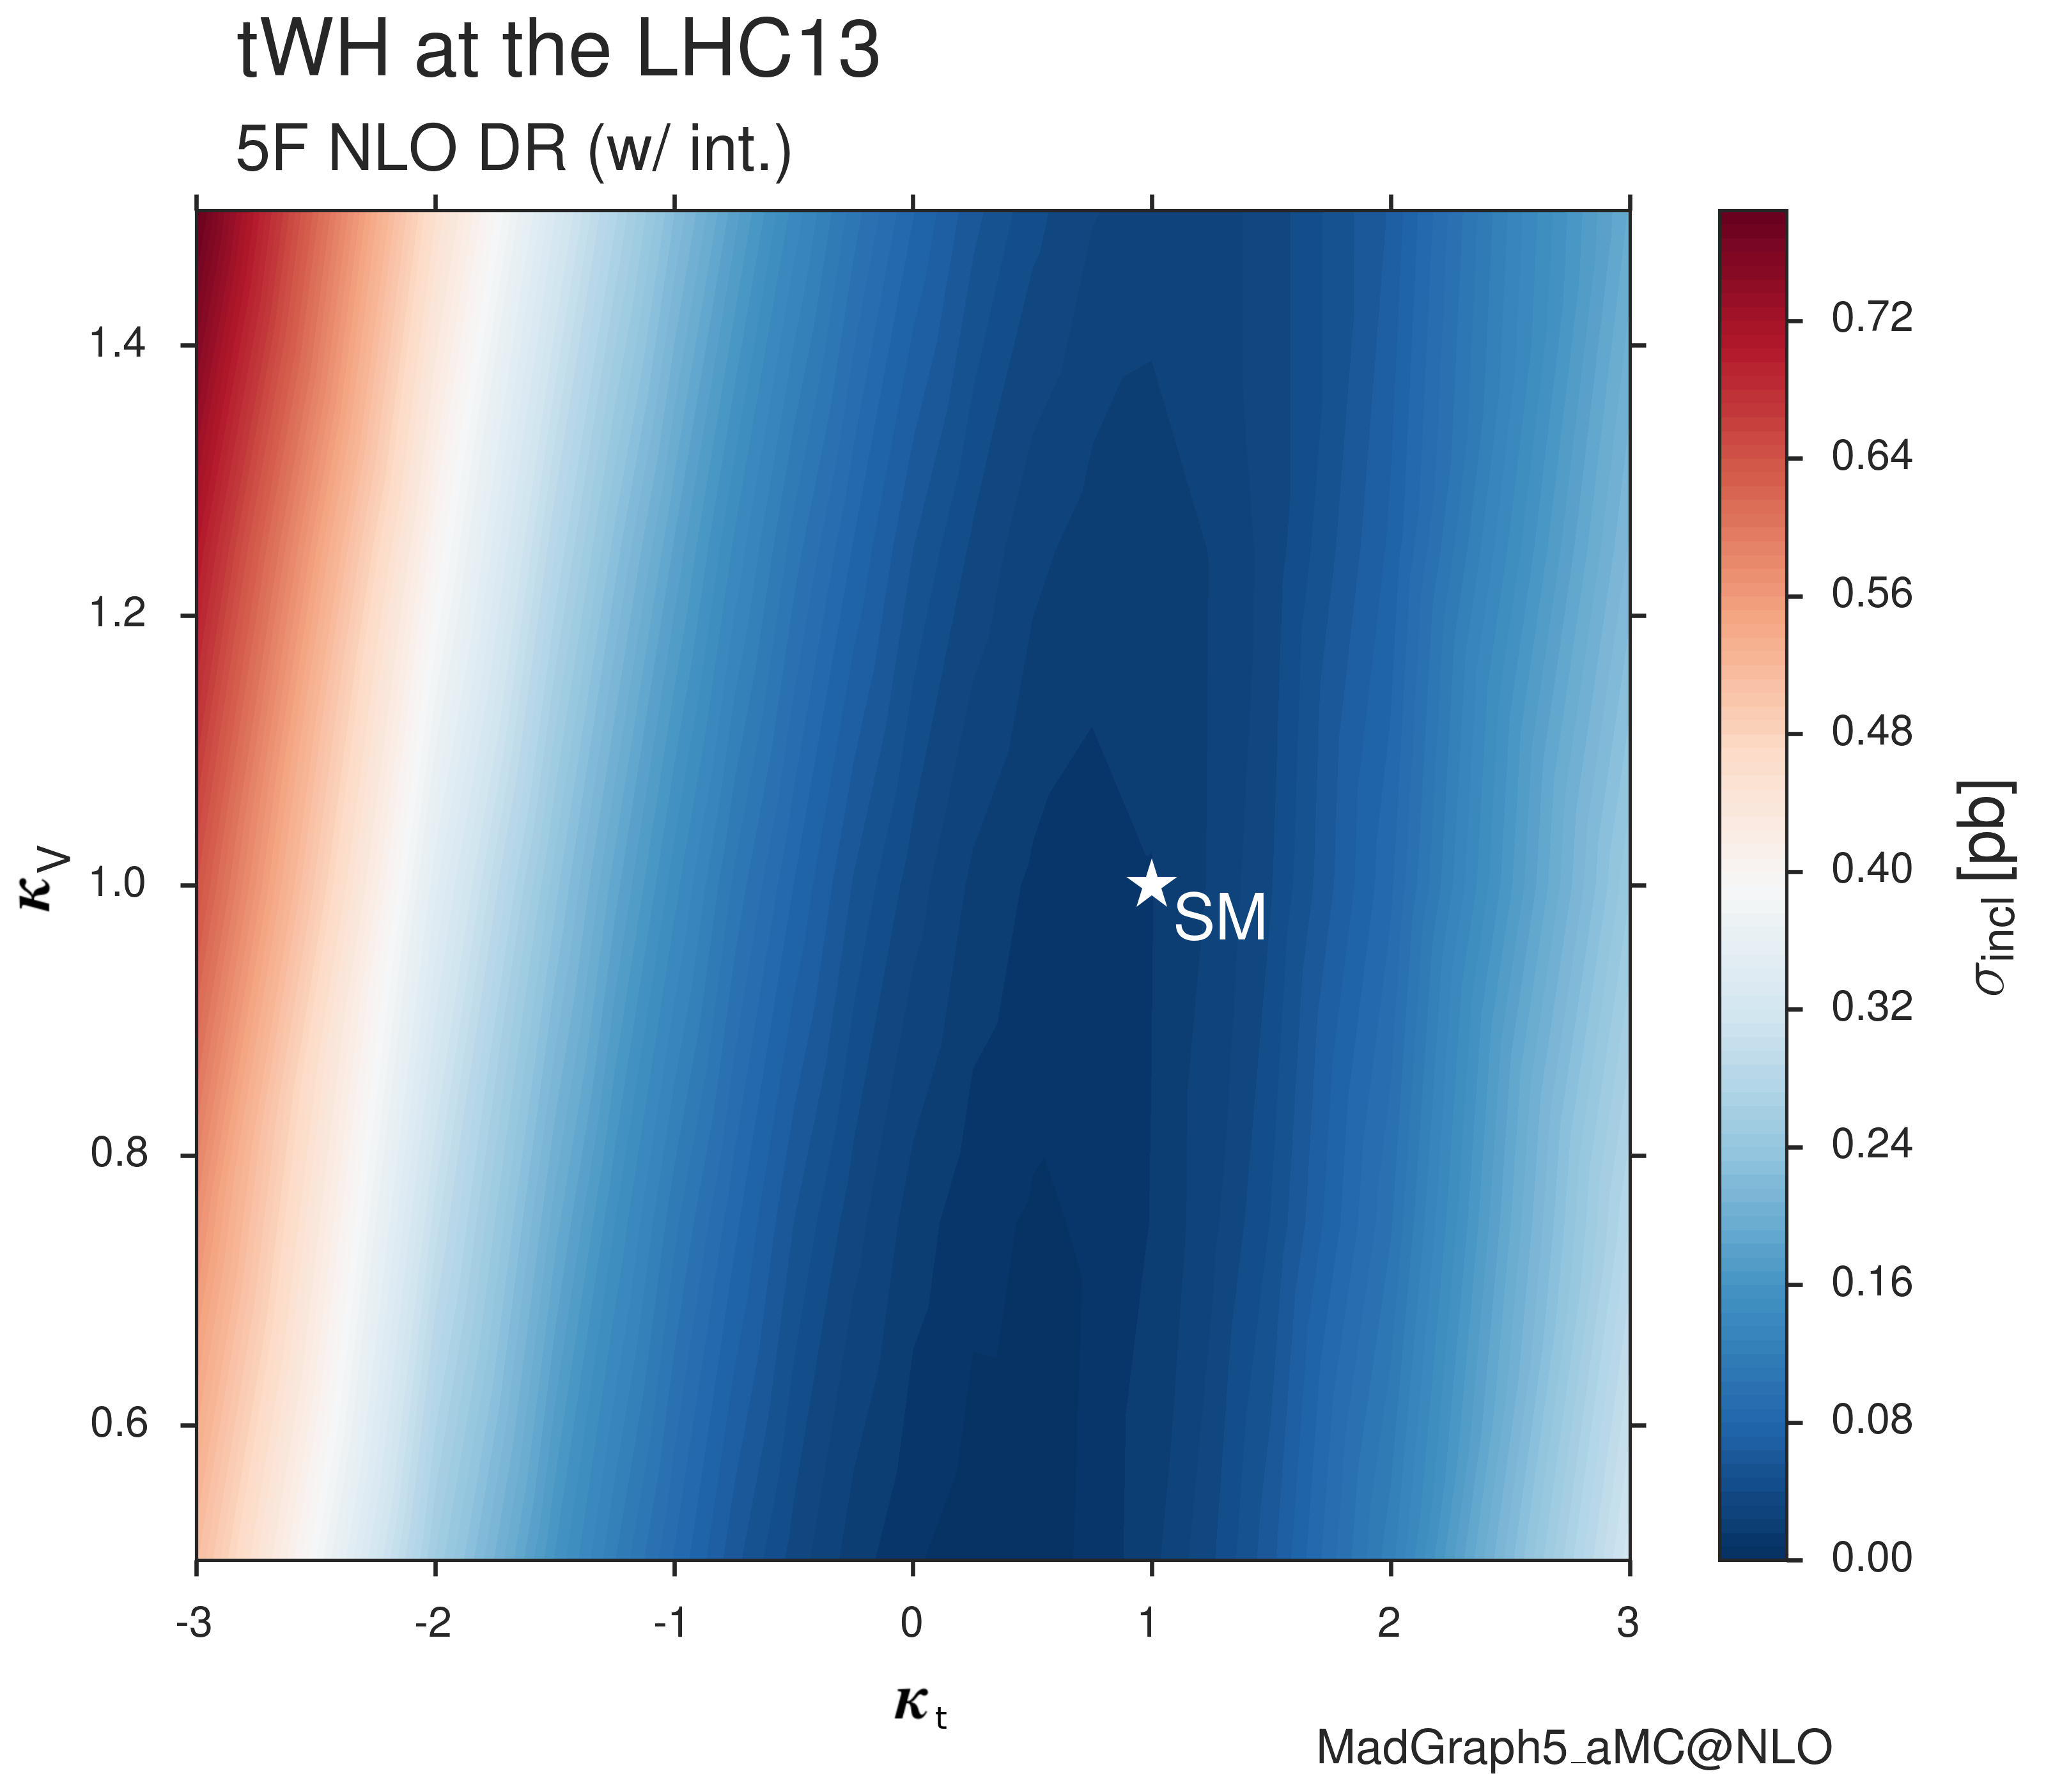
\includegraphics[width=0.49\textwidth]{tWH_xsec_cfcv} 
\caption[\tHq and \tHW cross section in the \Ct-\CV phase space]{\tHq and \tHW cross section in the \Ct-\CV phase space \cite{THQProdTwiki}.}
\label{fig:ktkv_phase_space}
\end{figure}

The \tHq and \tHW cross sections in the \Ct-\CV phase space are shown in Figure \ref{fig:ktkv_phase_space}. As said in Section \ref{sec:event_generation}, the \tHq sample was generated using the 4F scheme which provides a better description of the additional $b$ quark from the initial gluon splitting, while the \tHW sample was generated using the 5F scheme in order to remove its interference with \ttH at LO.


\subsubsection*{MC signal samples}\label{ssec:mc_signal}

The two signal samples, \tHq\ and \tHW, correspond to the \verb|RunIISummer16MiniAODv2| campaign produced with CMSSW\_80X; they were produced with \textsc{MG5\_}a\textsc{MC@NLO} (version 5.2.2.3), in LO mode at $\sqrt{s}=13$ TeV, and are normalized to NLO cross sections (see Table~\ref{tab:sigsamples}). The Higgs boson is assumed to be SM-like except for the values of its couplings to the top quark and W boson. Each sample was generated with a set of event weights corresponding to 51 different values of (\Ct, \CV) couplings, accessible in terms of LHE event weights as shown in Table ~\ref{tab:reweight}; however, the main interest is the $(\Ct=-1,\CV=1)$ case. 

\begin{table}[h]
\centering \small
\begin{tabular}{lll}
Sample & $\sigma$ [pb] & BF \\ \hline
\verb|/THQ_Hincl_13TeV-madgraph-pythia8_TuneCUETP8M1/|                  & 0.7927 & 0.324 \\
\verb|/THW_Hincl_13TeV-madgraph-pythia8_TuneCUETP8M1/|                  & 0.1472 & 1.0   \\\hline
\verb|/ttHJetToNonbb_M125_13TeV_amcatnloFXFX_madspin_pythia8_mWCutfix/|   & 0.2151 & 1.0 \\\hline
\end{tabular}
\caption[MC signal samples.]{MC signal samples used in this analysis; cross section and branching fraction are also listed ~\cite{THQProdTwiki}.}\label{tab:sigsamples}
\end{table}

The \ttH sample was produced using \textsc{AMC@NLO} interfaced to \textsc{PYTHIA} 8 for the parton shower, and is scaled to NLO cross sections.% The \ttH cross section depends quadratically on \Ct; however, in contrast to the \tHq and \tHW samples, the scaling is not performed during the sample generation process but in the analysis code since it was decided to include the \ttH process as a part of the signal in the course of the analysis.     

% add something about why tth is included as signal and why? if it is not sensitive to kt sign , 

\subsubsection*{MC background samples}

Several MC generators were used to generate the samples of the background processes. The dominant background sources (\ttbar, \ttW, \ttZ) were produced using \textsc{aMC@NLO} interfaced to PYTHIA8, and are scaled to NLO cross sections. Other minor background processes are simulated using POWHEG interfaced to PYTHIA, or bare PYTHIA as stated in the sample names in Table ~\ref{tab:bgsamples}. Pileup interactions are included in the simulation in order to reflect the observed multiplicity in data; the simulated events are weighted according to the actual pileup in data, estimated from the measured bunch-to-bunch instantaneous luminosity and the total inelastic cross section, 69.2 mb. All events are finally passed through a full simulation of the CMS detector using GEANT4, and reconstructed using the same algorithms as used for the data.
%______________________ object id ______________________
\section{Object Identification}\label{sec:ob_id}


In this section, the specific definitions of the physical objects in terms of the reconstruction parameters are presented; thus, the details provided summarize and complement the descriptions presented in previous chapters. The object reconstruction and selection strategy used in this thesis are inherited from the analyses in References \cite{CMS_AN_2016-211,CMS_AN_2017-029}.

\subsection{Lepton reconstruction and identification}

Two types of leptons are defined in this analysis: \ti{signal leptons} are those coming from $W, Z$ and $\tau$ decays which usually are isolated from other particles; \ti{background leptons} are defined as leptons produced in \bjet hadron decays, light-jets misidentification, and photon conversions; they are the same non-prompt leptons defined before. 

The process of reconstruction and identification of electron and muon candidates was described in chapter\ref{ch:gensimreco}, hence, the identification variables used in order to retain the highest possible efficiency for signal leptons while maximizing the rejection of background leptons are listed and described in the following sections \footnote{The studies performed to optimize the identification are far from the scope of this thesis, therefore, only general descriptions are provided.}.

The identification variables include not only observables related directly to the reconstructed leptons themselves, but also to the clustered energy deposits and charged particles in a cone around the lepton direction (jet-related variables); an initial loose preselection of leptons candidates is performed and then an MVA discriminator, referred to as \ti{lepton MVA} discriminator, is used to distinguish signal leptons from background leptons.

\subsubsection*{Muons}

The Physics Objects Groups (POG) at CMS are in charge of studying and defining the set of selection criteria applied in the course of reconstruction and identification of particles. These selection criteria are implemented in the CMS framework in the form of several object identification working points according to the stringency of the requirements.

The muon candidates are reconstructed by combining information from the tracker system and the muon detection system of CMS detector and the POG defined three working points for muon identification \ti{MuonID}\cite{muid};

\begin{itemize}
\item \ti{POG Loose Muon ID} is a particle identified as a muon by the PF event reconstruction and also reconstructed either as a global-muon or as an arbitrated tracker-muon. These identification criteria are designed to be highly efficient for prompt muons and for muons from heavy and light quark decays; they can be complemented by applying impact parameter cuts in analyses with prompt muon signals.
\item \ti{POG Medium Muon ID} is a Loose muon with additional track-quality and muon-quality (spatial matching between the individual measurements in the tracker and the muon system) requirements. These identification criteria are designed to be highly efficient in the identification of the muons coming from decay in flight of heavy quarks so that they can be separated from muons coming from B meson decays as well as prompt muons. An additional category \ti{MVA Prompt ID} is defined in these identification criteria directed to discriminated muons from B mesons and prompt muons (from W,Z and $\tau$ decays). The Medium ID (+ MVA Prompt ID) provides the same fake rate as the Tight Muon ID but a higher efficiency on prompt and B-decays muons \cite{medium_muon}.
\item \ti{POG Tight Muon ID} is a global muon with additional muon-quality requirements Tight Muon ID selects a subset of the PF muons.  
\end{itemize}

Only muons within the muon system acceptance $|\eta| < 2.4$ and minimum \pt  of 5 GeV are considered. %The requirements for each working point are listed in Table \ref{tab:muonid}. 

\subsubsection*{Electrons}

Electrons are reconstructed using information from the tracker and from the electromagnetic calorimeter and identified by an MVA algorithm (\ti{MVA eID} discriminant) using the shape of the calorimetric shower variables like the shape in \etac and \phic, the cluster circularity, widths along \etac and \phic; track-cluster matching variables relating the electron momentum at the point of closest approach to the beam spot ($p_{in}$), the electron momentum extrapolated to the surface of the ECAL from the track at the exit of the tracker ($p_{out}$), the \etac and \phic position of the supercluster (SC), the track \etac and \phic position extrapolated from the innermost track hit; and track quality variables like $\chi^2$ of the GSF tracks and the number of hits used by the GSF filter\cite{mva_eid1, mva_eid}.

A loose selection based on \etac-dependent cuts on this discriminant is used to preselect electron candidates; the full shape of the discriminant is used in the lepton MVA selection to separate signal leptons from background leptons (as described in Section \ref{sssec:leptonmva}).

In order to reject electrons from photon conversions, electron candidates with missing hits in the pixel tracker layers or matched to a conversion secondary vertex are discarded. Electrons are selected for the analysis if they have \pt > 7 GeV and are located within the tracker system acceptance region ($|\eta|$ < 2.5). %All the electron selection criteria are listed in Table\ref{tab:eleid}.

\subsubsection*{Lepton vertexing and pile-up rejection}

The impact parameter in the transverse plane $d_0$, impact parameter along the $z$-axis $d_z$, and the impact parameter significance in the detector space $SIP_{3D}$ are considered to perform the identification and rejection of pile-up, misreconstructed tracks, and background leptons from b-hadron decays; pile-up and misreconstructed track mitigation is achieved by imposing loose cuts on the impact parameter variables. The full shape of those variables is used in a lepton MVA classifier to achieve the best separation between the signal and the background leptons.

\subsubsection*{Lepton isolation}

PF is able to recognize leptons from two different sources: on one side, leptons from the decays of heavy particles, such as W and Z bosons, which are normally isolated in space from the hadronic activity in the event; on the other side, leptons from decays of hadrons and jets misidentified as leptons, which are not isolated as the former. For highly boosted systems, like the lepton and the $b$-jet generated in the semileptonic decay of a boosted top, the decay products tend to be more closer and sometimes they even overlap; thus, the PF standard definition of isolation in terms of the separation $\Delta R$ between lepton candidates (l) and other PF objects (i) in the \etac-\phic plane,

\beqn
\Delta R =\sqrt{( \eta^l - \eta^i)^2 + (\phi^l - \phi^i)^2} < 0.3
\eeqn

\noindent which considers all the neutral, charged hadrons and photons in a cone around the leptons, is refocused to the local isolation of the leptons through the mini-isolation $I_{mini}$ \cite{i_mini} defined as the sum of particle flow candidates \pt within a cone around the lepton, corrected for the effects of pileup and divided by the lepton \pt
\beqn
I_{mini} =\frac{\displaystyle\sum_{R} p_T(h^\pm) - \textrm{max}\left(0,\displaystyle\sum_R p_T(h^0) + p_T(\gamma)-\rho \mathcal{A}\left(\frac{R}{0.3}\right)^2\right)}{p_T(l)}
\eeqn

\noindent where $\rho$ is the pileup energy density, and $h^\pm, h^0, \gamma, l,$ represent the charged hadron, neutral hadrons, photons, and the lepton, respectively. The radius R of the cone depends on the \pt of the lepton according to 
\beqn
R = \frac{10\ \textrm{GeV}}{\textrm{min}[\textrm{max}(p_T(l), 50\ \textrm{GeV}), 200\ \textrm{GeV}]},
\eeqn

The \pt dependence of the cone size allows for greater signal efficiency. Setting a cut on $I_{mini}$ below a given threshold ensures that the lepton is locally isolated, even in boosted systems. The effect of pileup is mitigated using the so-called effective area correction $\mathcal{A}$ listed in Table ~\ref{tab:pileup_area}. 

\begin{table}[!htbp]
\centering
\small
\begin{tabular}{ccc}\hline
$|\eta|$ range & $\mathcal{A}$(e) neutral/charged & $\mathcal{A}$ ($\mu$) neutral/charged \\\hline
0.0 - 0.8      & 0.1607 / 0.0188                  & 0.1322 / 0.0191 \\
0.8 - 1.3      & 0.1579 / 0.0188                  & 0.1137 / 0.0170 \\
1.3 - 2.0      & 0.1120 / 0.0135                  & 0.0883 / 0.0146 \\
2.0 - 2.2      & 0.1228 / 0.0135                  & 0.0865 / 0.0111 \\
2.2 - 2.5      & 0.2156 / 0.0105                  & 0.1214 / 0.0091 \\ \hline
\end{tabular}
\caption[Effective areas, for electrons and muons.]{ Effective areas, for electrons and muons used to mitigate the effect of pileup by using the so-called effective area correction.}
\label{tab:pileup_area}
\end{table}

A loose cut on $I_{mini}$ is applied to pre-select the muon and electron candidates; however, the full shape is used in the lepton MVA discriminator when performing the signal lepton selection.

\subsubsection*{Jet-related variables}

In order to reject misidentified leptons from $b-$jets, mostly coming from tt+jets, Drell-Yan+jets, and W+jets events, the vertexing and isolation described in previous sections are complemented with additional variables related to the closest reconstructed jet to the lepton, \ie, the PF jets reconstructed\footnote{Charged hadrons from PU vertices are not removed prior to the jet clustering.} around the leptons with $\Delta R=\sqrt{( \eta^l - \eta^{jet})^2 + (\phi^l - \phi^{jet})^2} < 0.5$. The identification variables used in the lepton MVA discriminator are the ratio $\pt^l/\pt^{jet}$, the CSV b-tagging discriminator value of the jet, the number of charged tracks of the jet, and the relative \pt given by

\beqn
p_T^{rel}=\frac{(\vec{p}_{jet}-\vec{p}_l)\cdot\vec{p}_l}{||\vec{p}_{jet} - \vec{p}_l||}.
\eeqn


\subsubsection*{LeptonMVA discriminator}\label{sssec:leptonmva}

Electrons and muons passing the basic selection process described above are referred to as \ti{loose leptons}. Additional discrimination between signal leptons and background leptons is crucial considering that the rate of \ttbar production is much larger than the signal, hence, an overwhelming background from \ttbar production is present. To maximally exploit the available information in each event to that end, the dedicated lepton MVA discriminator, based on a boosted decision tree (BDT) algorithm, has been built so that all the identification variables can be used together.

The lepton MVA discriminator training is performed using simulated signal Loose leptons from the \ttH MC sample and non-prompt leptons from the \ttbar+jets MC sample, separately for muons and electrons. \ttbar background contribution gets reduced because it is not possible to have two same-sign prompt leptons in \ttbar, so one of them has to be non-prompt, therefore, it gets suppressed by a leptonMVA cut.

The input variables used include vertexing, isolation and jet-related variables, the \pt and \etac of the lepton, the electron MVA eID discriminator and the muon segment-compatibility variables. An additional requirement known as the \ti{tight-charge} requirement is imposed by comparing two independent measurements of the charge, one using the ECAL supercluster position and the other from the tracker as described in Section \ref{subsubsec:part_id_reco}; thus, the consistency in the measurements of the electron charge is ensured so that events with a wrong electron charge assignment are rejected; this variable is particularly used in the $2lss$ channel to suppress opposite-sign events for which the charge of one of the leptons has been mismeasured. The tight-charge requirement for muons is represented by the requirement of a consistently well measured track transverse momentum given by $\Delta p_T/p_T < 0.2$.          
Leptons are selected for the final analysis if they pass a given threshold of the BDT output, and are referred to as \ti{tight leptons} in the following.          

The validation of the lepton MVA algorithm and the lepton identification variables is performed using data in various control regions; the details about that validation are not discussed here but can be found in Reference \cite{CMS_AN_2017-029}. 

\subsubsection*{Selection definitions}

Electron and muon object identification is defined in three different sets of selections criteria; the \emph{Loose}, \emph{Fakeable Object}, and \emph{Tight} selection. These three levels of selection are designed to serve for event level vetoes, the fake rate estimation application region (see Section \ref{ssec:fake_rate}), and the final signal selection, respectively. The \pt of fakeable objects is defined as $0.85\times\pt(\mathrm{jet})$, where the jet is the one associated to the lepton object. This mitigates the dependence of the fake rate on the momentum of the fakeable object and thereby improves the precision of the method. 

Tables~\ref{tab:muonIDs} and~\ref{tab:eleIDs} list the full criteria for the different selections of muons and electrons.


\begin{table}[!htbp]
\centering
\small
\begin{tabular}{cccc}\hline
Cut                    & Loose      & Fakeable object    & Tight \\
\hline
$|\eta| < 2.4$         & \checkmark & \checkmark         & \checkmark \\
$\pt$                  & $>5$\ GeV   & $>15$\ GeV          & $>15$\ GeV\\
$|d_{xy}| < 0.05$ (cm) & \checkmark & \checkmark         & \checkmark \\
$|d_z| < 0.1$ (cm)     & \checkmark & \checkmark         & \checkmark \\
$\text{SIP}_{3D} < 8$  & \checkmark & \checkmark         & \checkmark \\
\miniIso $< 0.4$       & \checkmark & \checkmark         & \checkmark \\
is Loose Muon          & \checkmark & \checkmark         & \checkmark \\
%\ptRatio              & --         & $>0.3\dagger$ / -- & -- \\
jet CSV                & --         & $< 0.8484$         & $ < 0.8484$ \\
%mva electron ID       & --         & $\ddagger$         & -- \\
is Medium Muon         & --         & --                 & \checkmark \\
tight-charge           & --         & --                 & \checkmark \\
lepMVA $> 0.90$        & --         & --                 & \checkmark \\
\hline
\end{tabular}
\caption[Requirements on each of the three muon selections.]{Requirements on each of the three muon selections. In the cases where the cut values change between the selections, those values are listed in the table. Otherwise, whether the cut is applied is indicated.}
\label{tab:muonIDs}
\end{table}

\begin{table}
\centering
\small
\resizebox{1.0\linewidth}{!}{
\begin{tabular}{cccc}\hline
Cut                                             & Loose      & Fakeable Object              & Tight \\\hline
$|\eta| < 2.5$                                  & \checkmark & \checkmark                   & \checkmark \\
$\pt$                                           & $>7$\ GeV   & $>15$\ GeV                    & $>15$\ GeV      \\
$|d_{xy}| < 0.05$ (cm)                          & \checkmark & \checkmark                   & \checkmark \\
$|d_z| < 0.1$ (cm)                              & \checkmark & \checkmark                   & \checkmark \\
$\text{SIP}_{3D} < 8$                           & \checkmark & \checkmark                   & \checkmark \\
\miniIso $< 0.4$                                & \checkmark & \checkmark                   & \checkmark \\
MVA eID $> (0.0, 0.0, 0.7)$                     & \checkmark & \checkmark                   & \checkmark \\
$\sigma_{i\eta i\eta} <(0.011,0.011,0.030)$     & --         & \checkmark                   & \checkmark \\ %   & for corr. $\pt>30$ & for corr. $\pt>30$ \\
H/E $< (0.10,0.10,0.07)$                        & --         & \checkmark                   & \checkmark \\ %   & for corr. $\pt>30$ & for corr. $\pt>30$ \\
$\Delta\eta_{\textrm in} < (0.01, 0.01, 0.008)$ & --         & \checkmark                   & \checkmark \\ %   & for corr. $\pt>30$ & for corr. $\pt>30$ \\
$\Delta\phi_{\textrm in} < (0.04, 0.04, 0.07)$  & --         & \checkmark                   & \checkmark \\ %   & for corr. $\pt>30$ & for corr. $\pt>30$ \\
$-0.05 < 1/E-1/p < (0.010,0.010,0.005)$         & --         & \checkmark                   & \checkmark \\ %   & for corr. $\pt>30$ & for corr. $\pt>30$ \\
\ptRatio                                        & --         & $>0.5^\dagger$ / --           & -- \\
jet CSV                                         & --         & $< 0.3^\dagger$ / $< 0.8484$ & $ < 0.8484$ \\
tight-charge                                    & --         & --                           & \checkmark \\
conversion rejection                            & --         & --                           & \checkmark \\
Number of missing hits                          & $<2$       & $== 0$                       & $== 0$ \\
lepton MVA $> 0.90$                             & --         & --                           & \checkmark \\\hline
\end{tabular}}
\caption[Criteria for each of the three electron selections.]{Criteria for each of the three electron selections. In cases where the cut values change between selections, those values are listed in the table. Otherwise, whether the cut is applied is indicated. In some cases, the cut values change for different $\eta$ ranges. These ranges are $0 < |\eta| < 0.8$, $0.8 < |\eta| < 1.479$, and $1.479 < |\eta| < 2.5$ and the respective cut values are given in the form (value$_1$, value$_2$, value$_3$). For the two \ptRatio\ and CSV rows, the cuts marked with a $\dagger$ are applied to leptons that fail the lepton MVA cut, while the loose cut value is applied to those that pass the lepton MVA cut.}
\label{tab:eleIDs}
\end{table}

In addition to the previously defined requirements for jets, they are required to be separated from any lepton candidates passing the fakeable object selections by $\Delta\mathrm{R}>0.4$.

\subsection{Lepton selection efficiency}

\begin{figure}[!hb]
\centering
  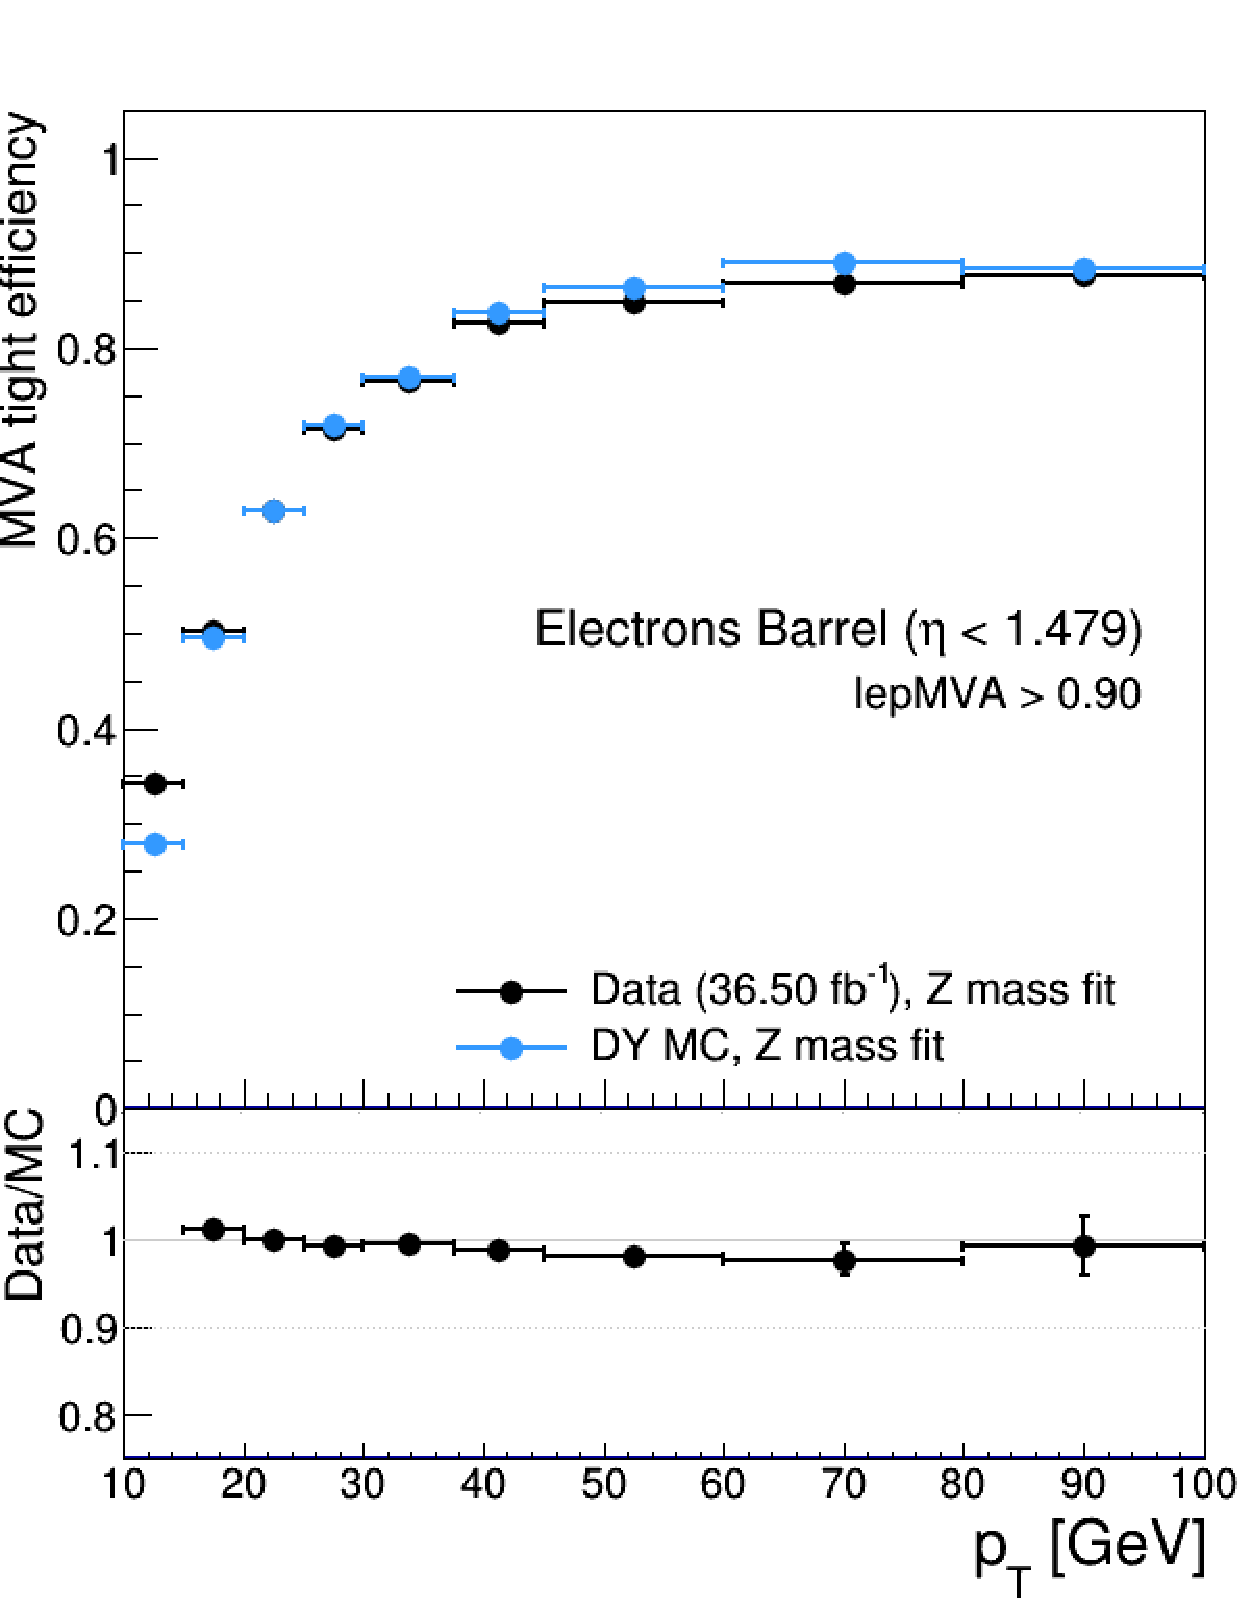
\includegraphics[width=0.4\linewidth]{lepmva_efficiency/tnp_eff_eb_2lss_pt.pdf}
  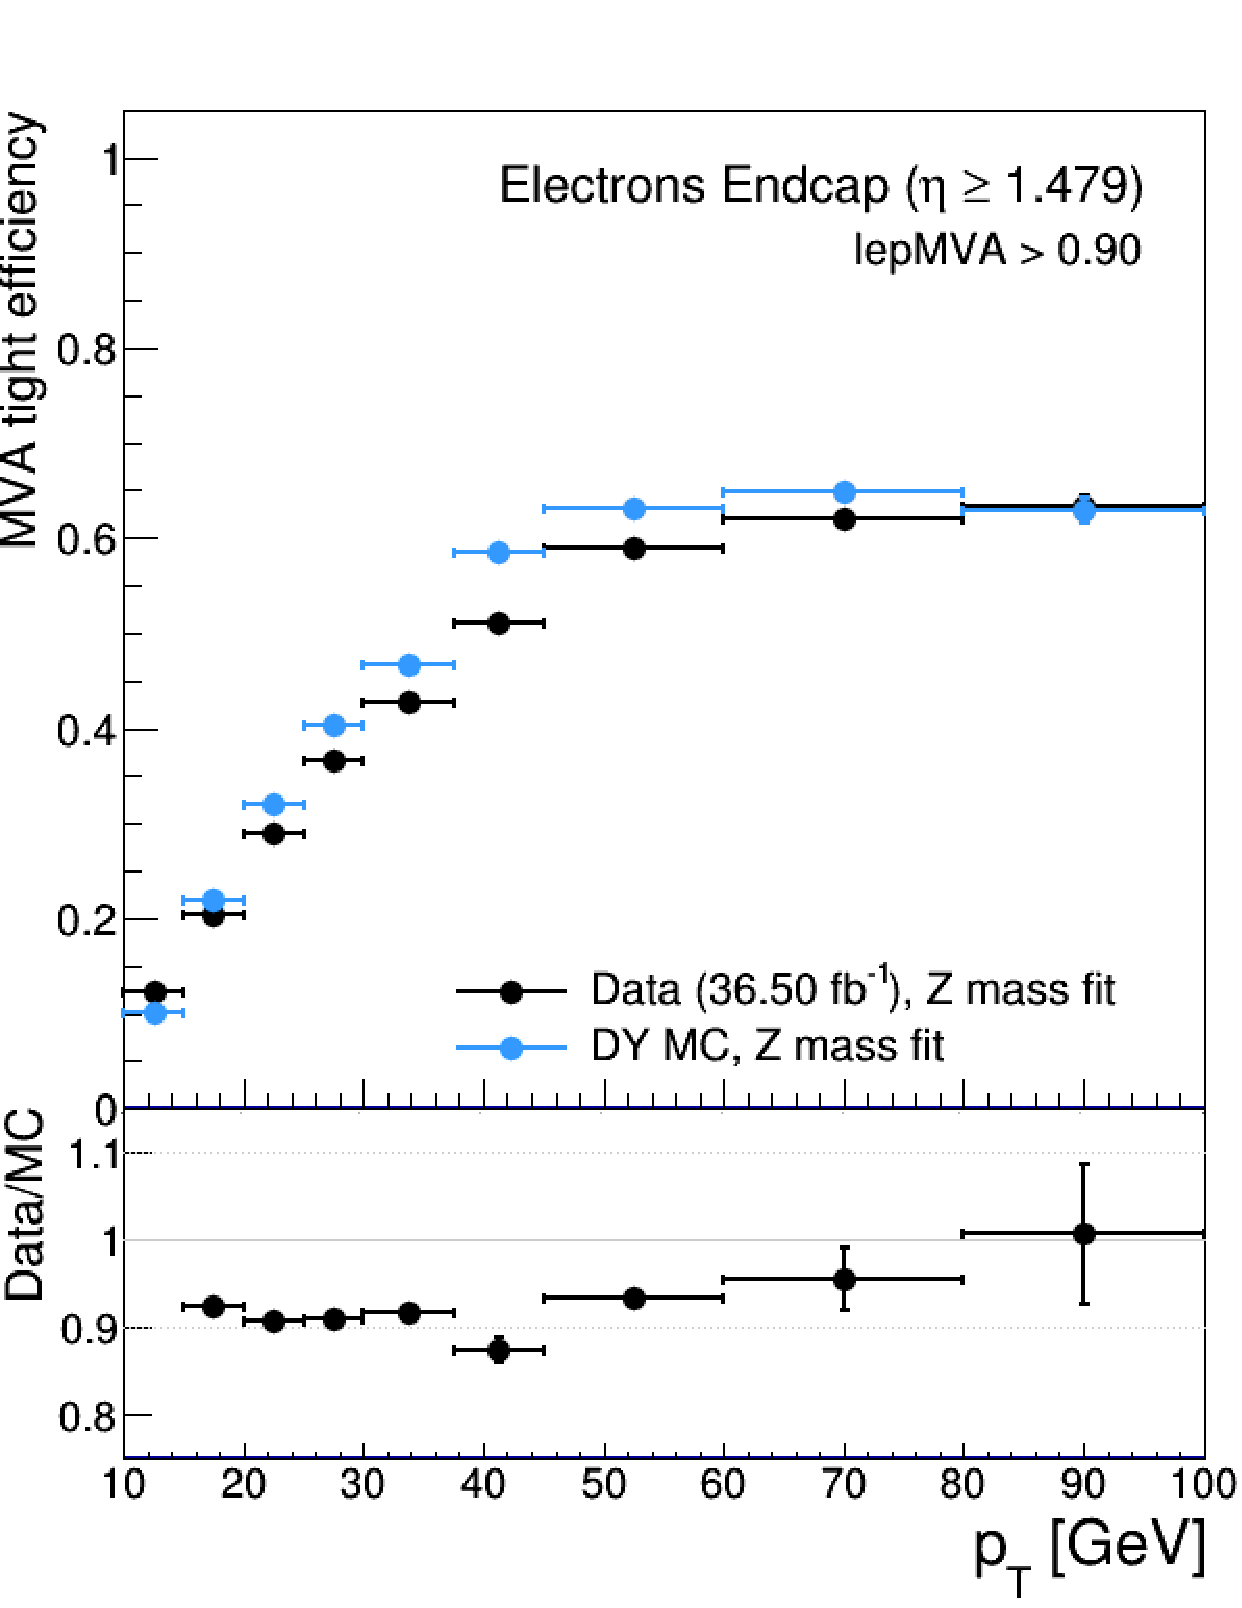
\includegraphics[width=0.4\linewidth]{lepmva_efficiency/tnp_eff_ee_2lss_pt.pdf}\\
  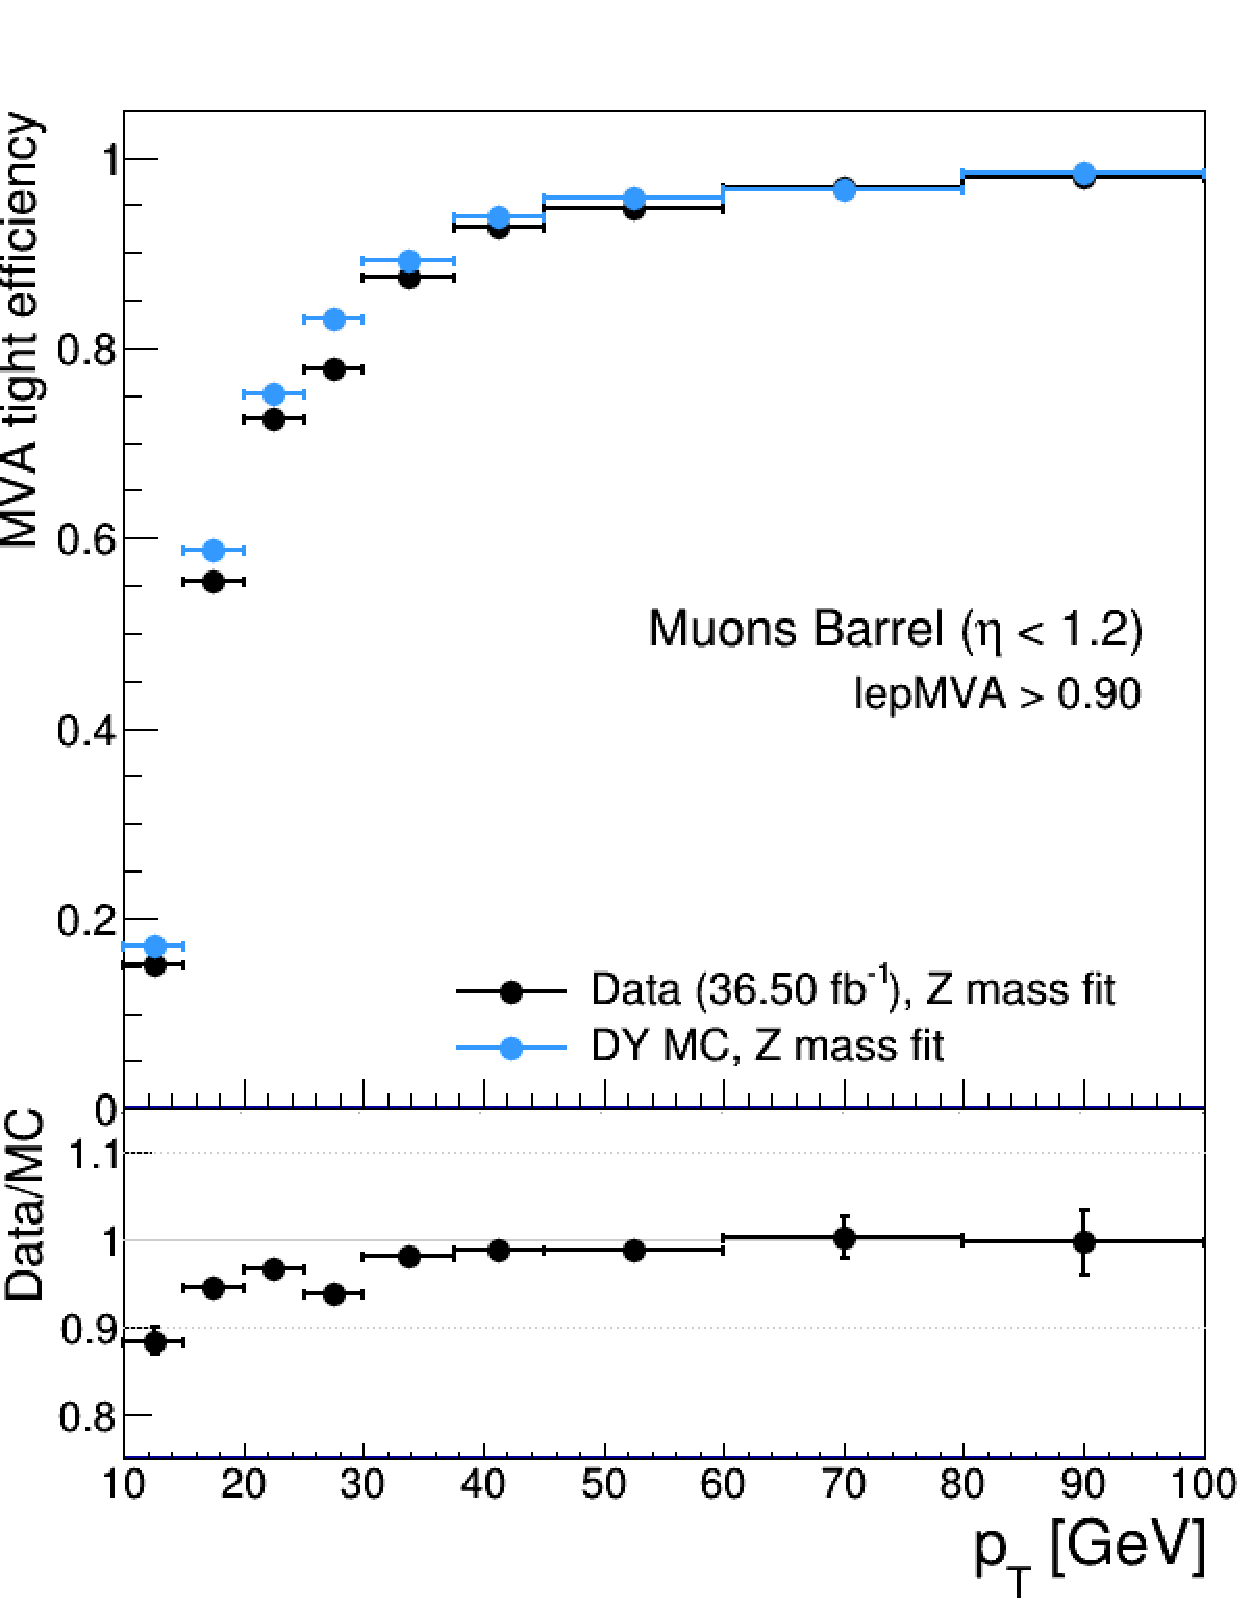
\includegraphics[width=0.4\linewidth]{lepmva_efficiency/tnp_eff_mb_2lss_pt.pdf}
  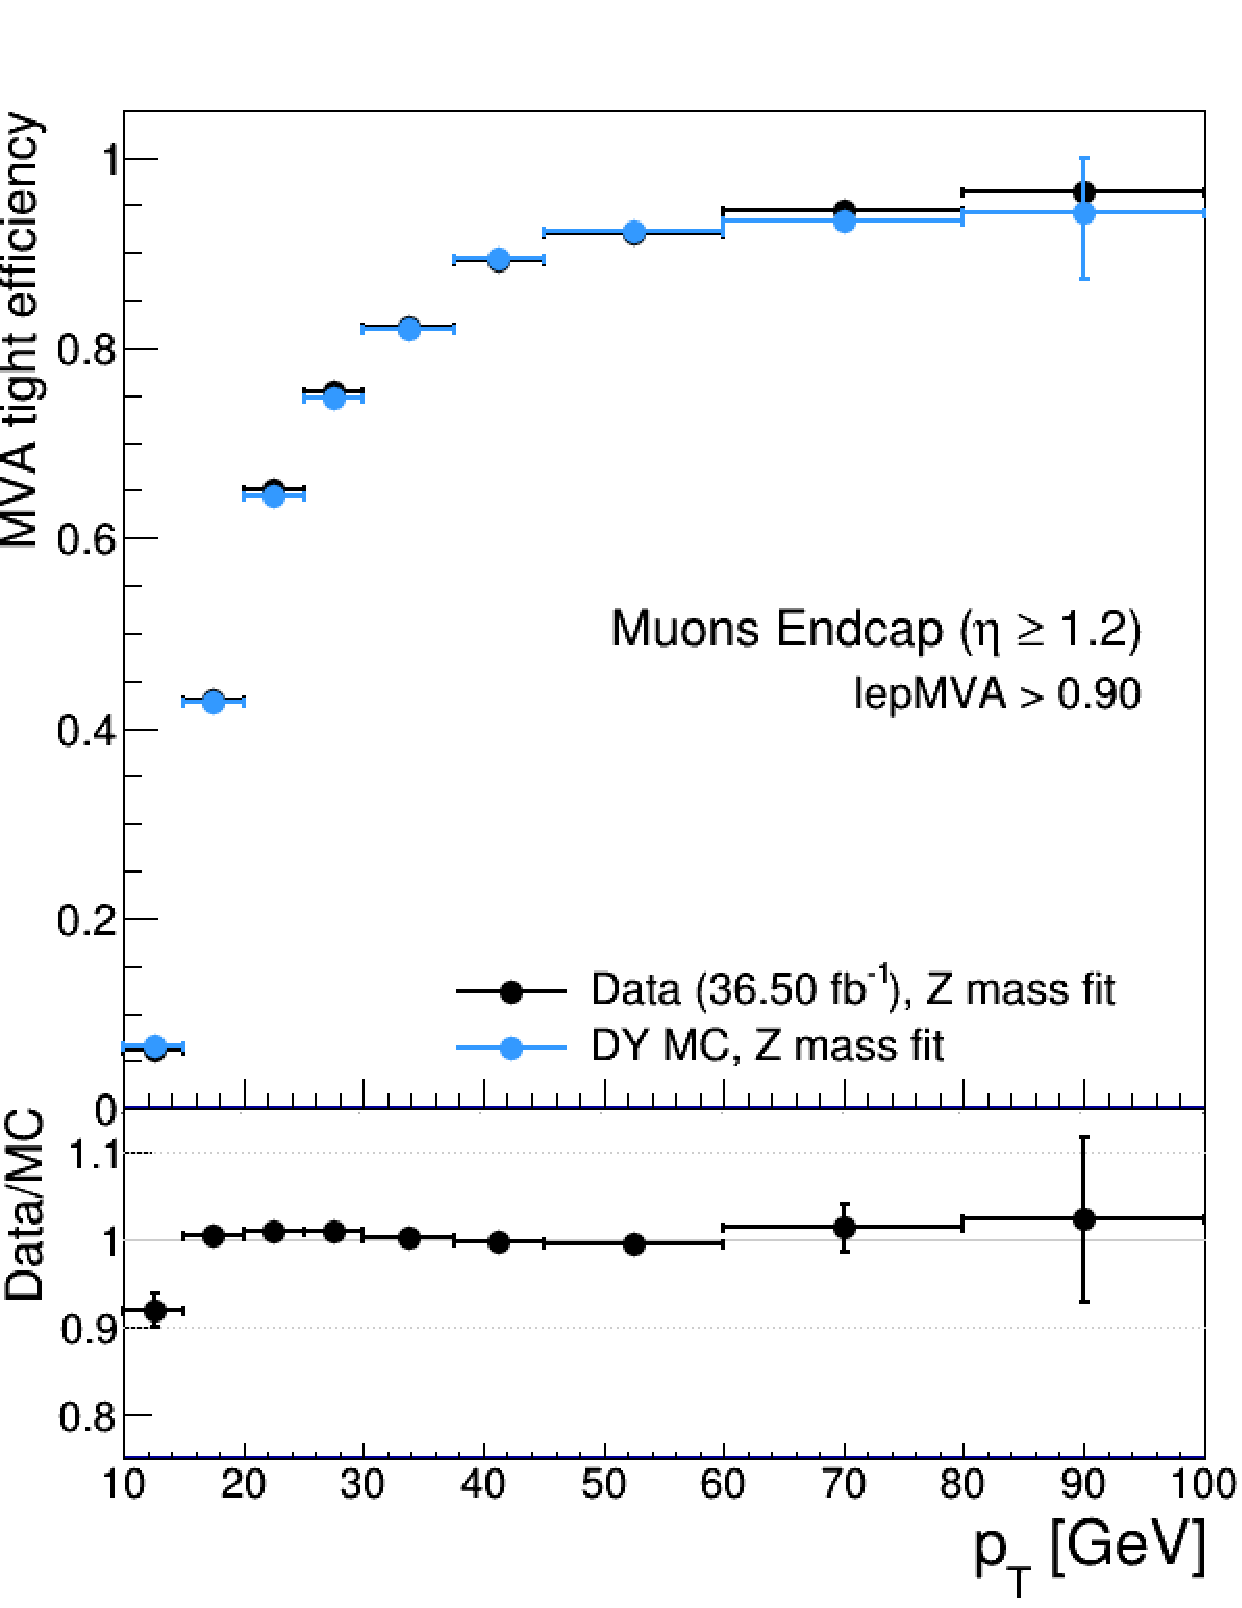
\includegraphics[width=0.4\linewidth]{lepmva_efficiency/tnp_eff_me_2lss_pt.pdf}
\caption[Tight vs loose lepton selection efficiencies in the $2lss$ channel.]{Tight vs loose selection efficiencies for electrons (top), and muons (bottom), for the $2lss$ definition, \ie, including the tight-charge requirement. The lower panes show the data/MC ratios.}
\label{fig:2lss_eff}
\end{figure}

\begin{figure}[!ht]
\centering
  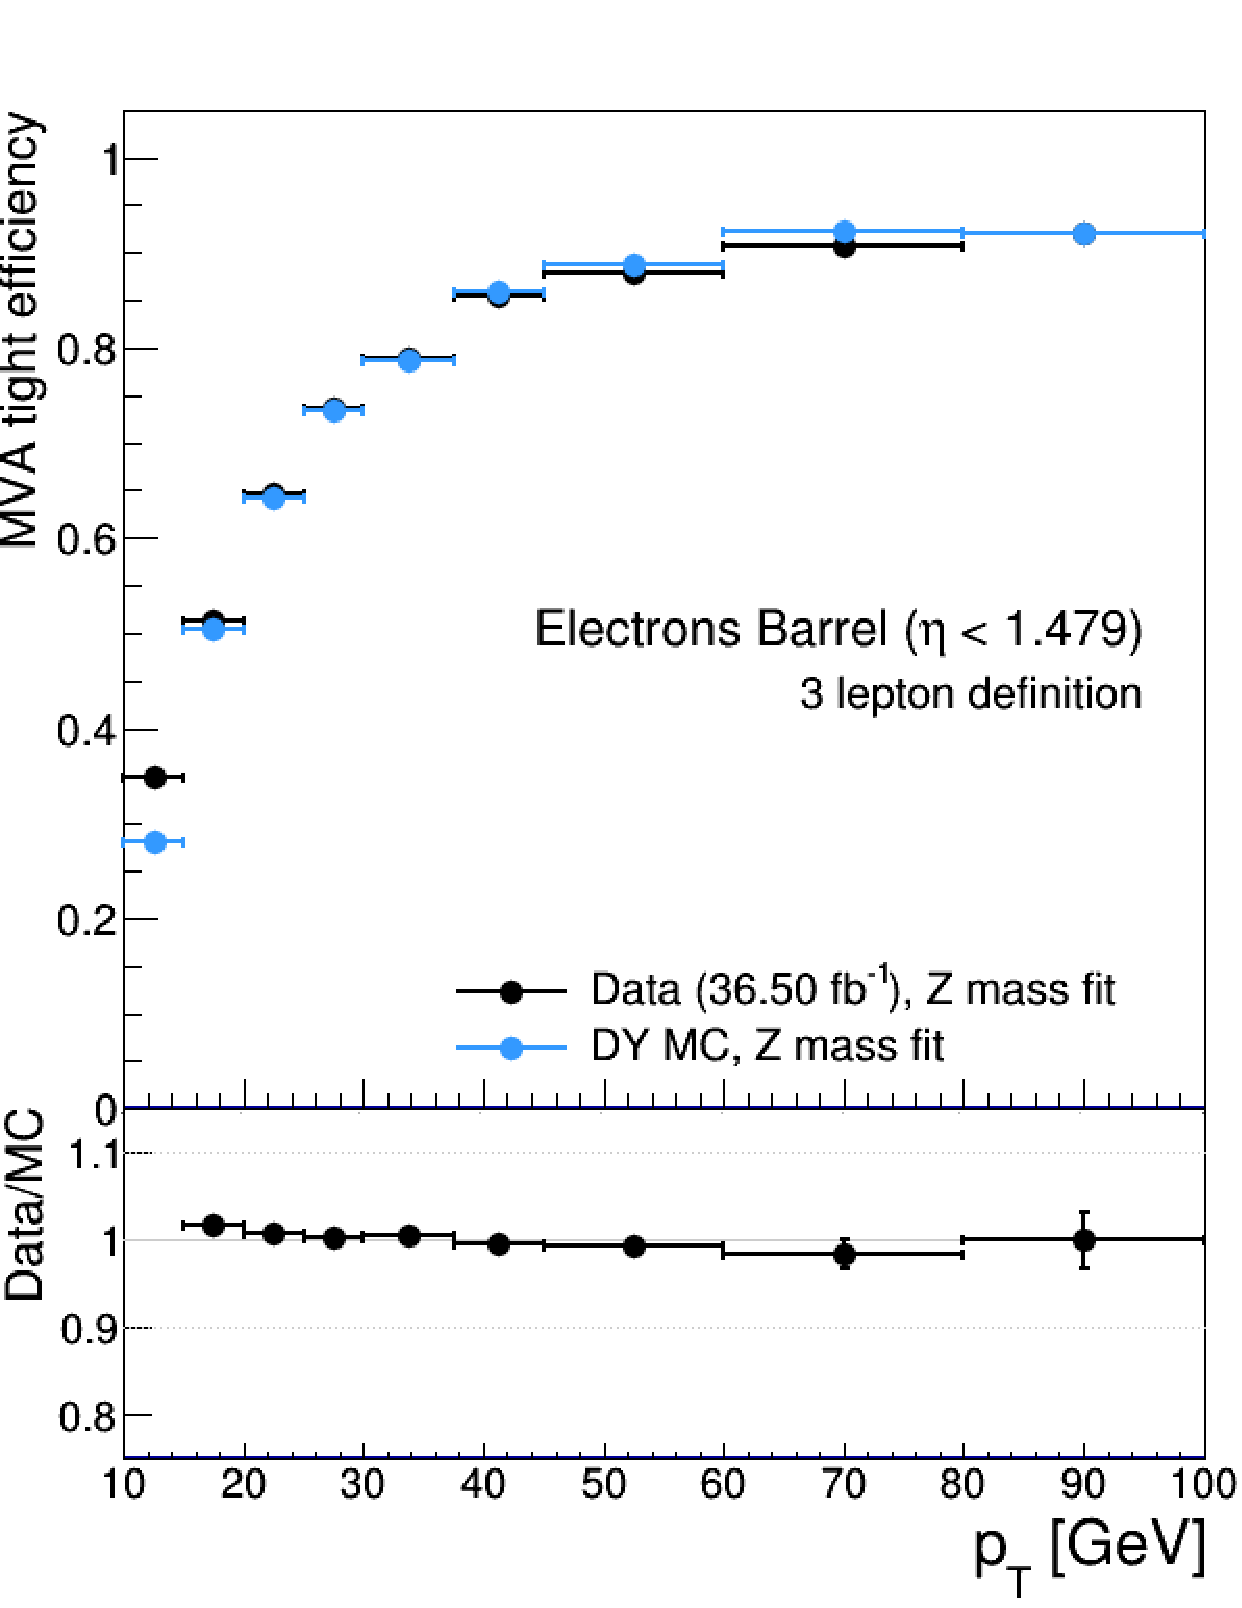
\includegraphics[width=0.4\linewidth]{lepmva_efficiency/tnp_eff_eb_3l_pt.pdf}
  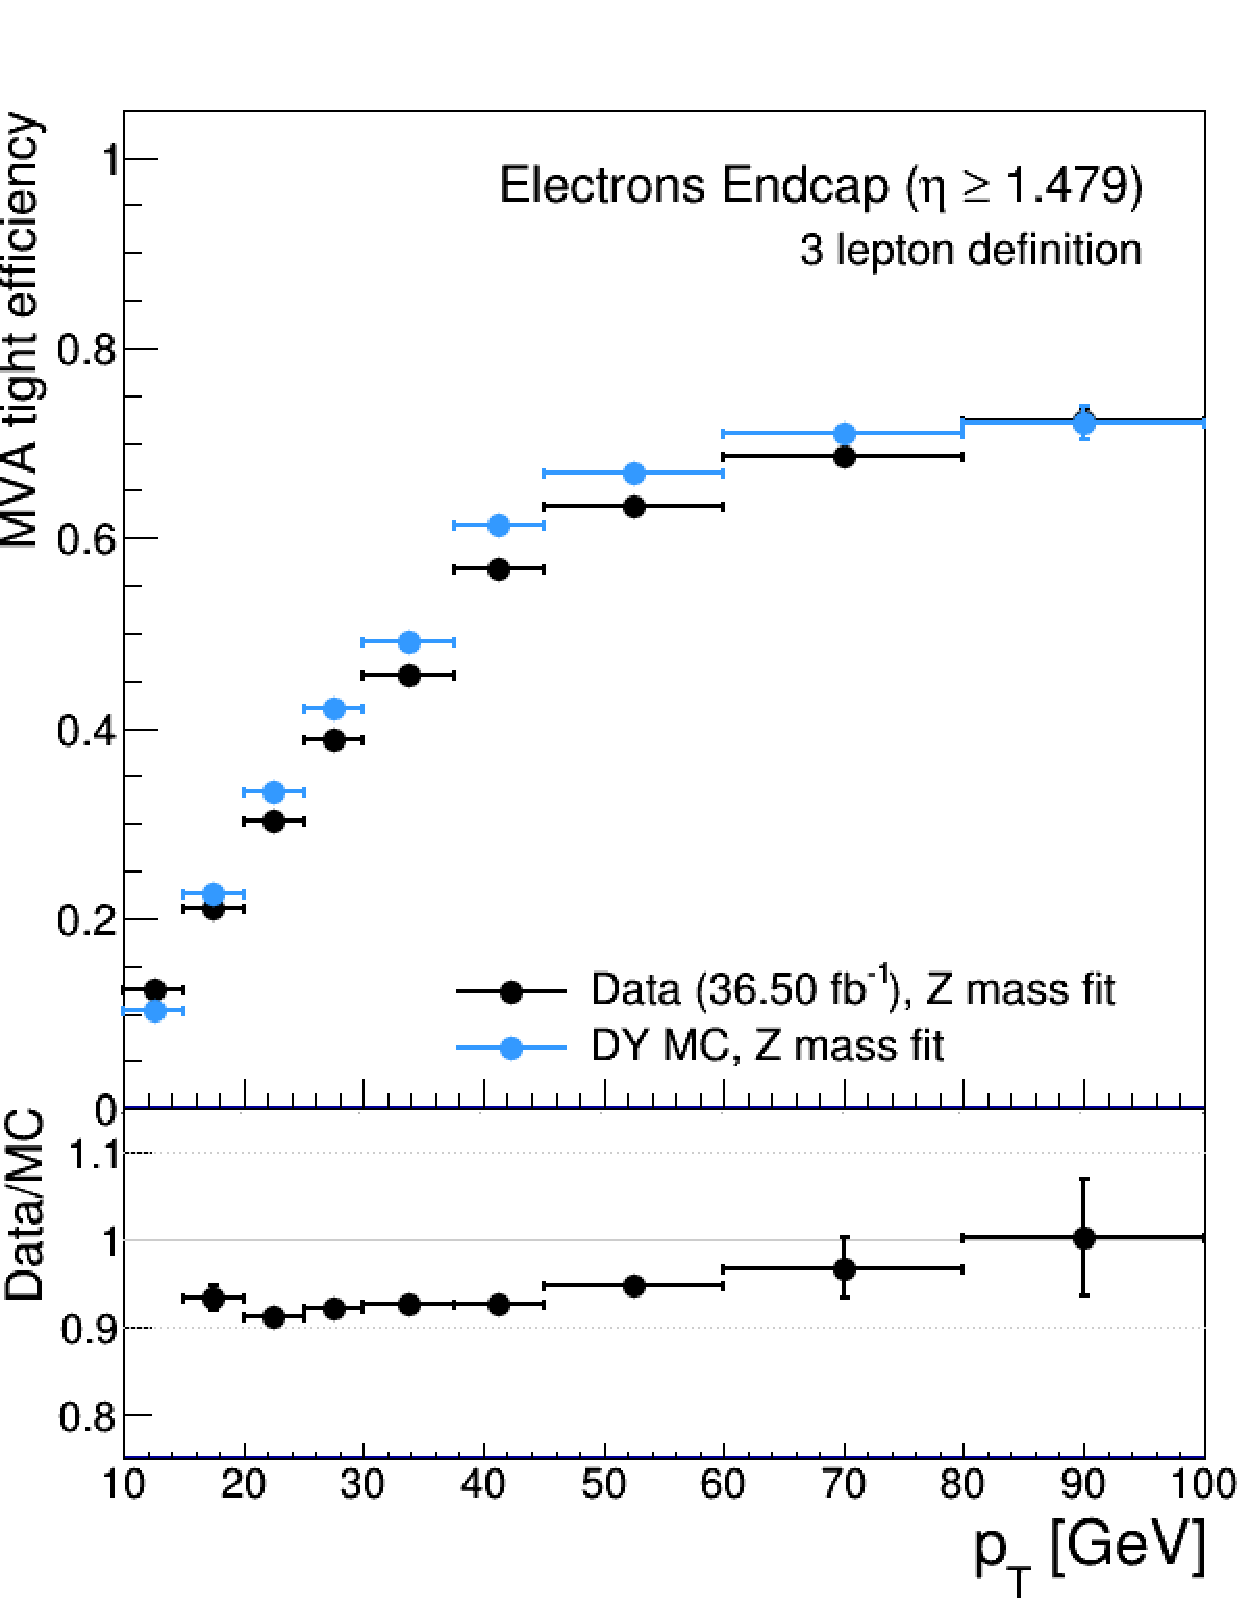
\includegraphics[width=0.4\linewidth]{lepmva_efficiency/tnp_eff_ee_3l_pt.pdf}\\
  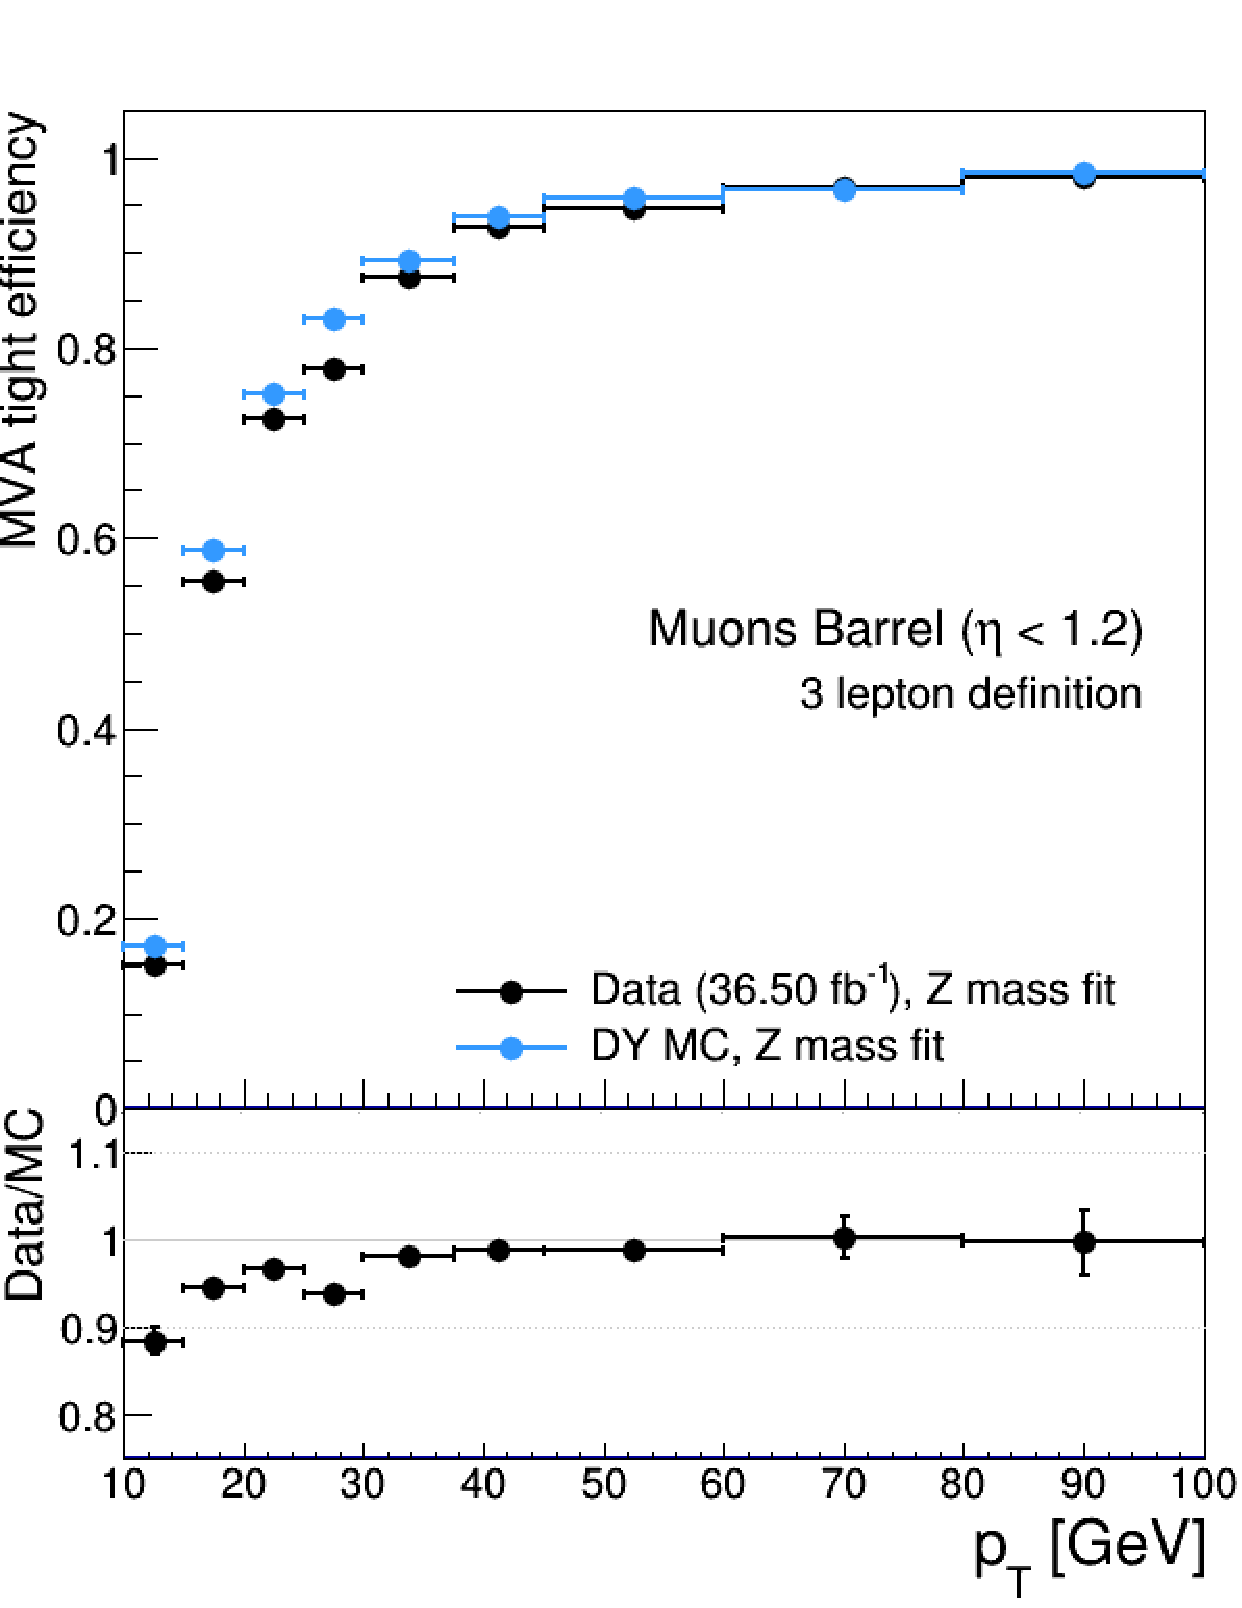
\includegraphics[width=0.4\linewidth]{lepmva_efficiency/tnp_eff_mb_3l_pt.pdf}
  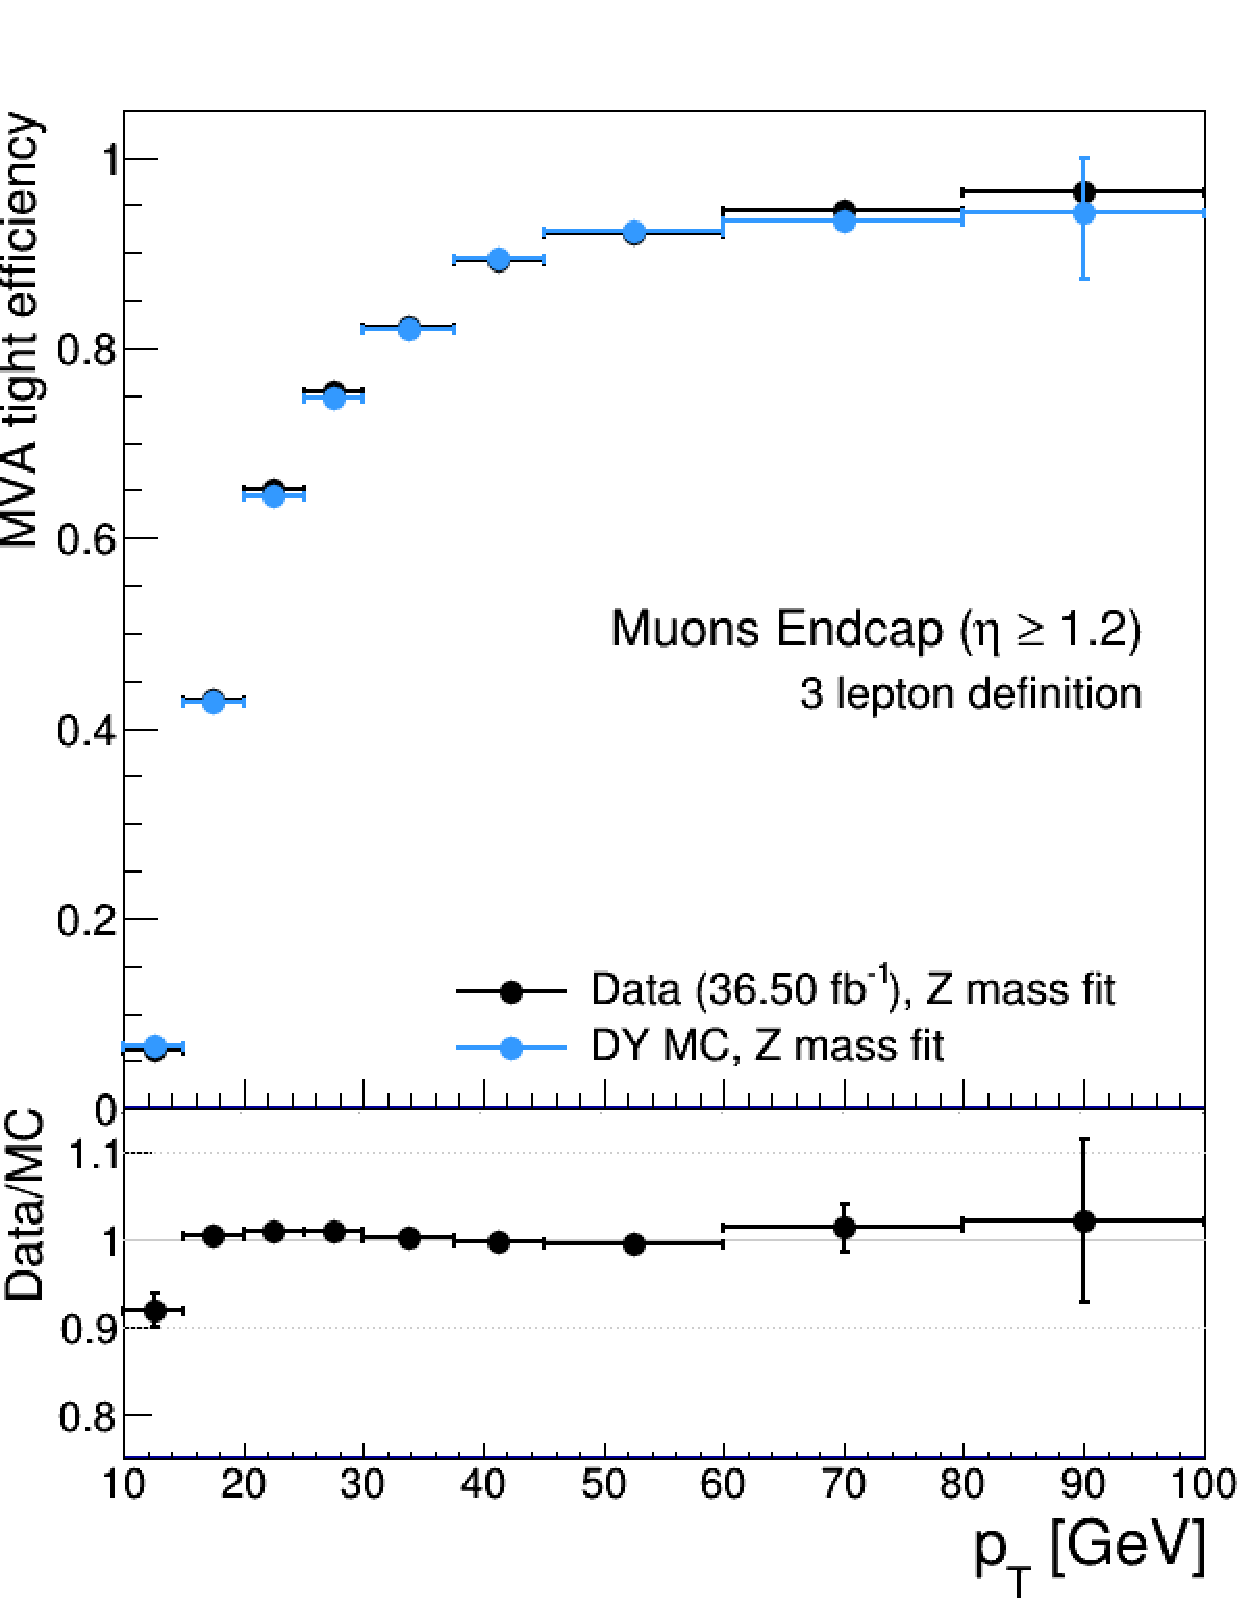
\includegraphics[width=0.4\linewidth]{lepmva_efficiency/tnp_eff_me_3l_pt.pdf}
\caption[Tight vs loose lepton selection efficiencies in the $3l$ channel.]{Tight vs loose selection efficiencies for electrons (top), and muons (bottom), for the $3l$ channel not including the tight-charge requirement. The lower panes show the data/MC ratios.}
\label{fig:3l_eff}
\end{figure}

Efficiencies of reconstructing and selecting loose leptons are measured both for muons and electrons using a tag and probe method on both data and MC, using $Z\rightarrow\ell^{+}\ell^{-}$ \cite{tnp}. The scale factors are derived from the ratio of efficiencies $\varepsilon_{i}(p_T, \eta)$ measured for a given lepton in data/MC, according to 
\beqn
\rho(p_T, \eta)= \frac{\varepsilon_{data}(p_T, \eta)}{\varepsilon_{MC}(p_T, \eta)}.
\eeqn

The scale factor for each event is used to correct the weight of the event in the full sample; therefore, the full simulation correction is given by the product of all the individual scale factors. The scale factors used in this thesis are inherited from Reference \cite{CMS_AN_2017-029} which in turns inherited them from leptonic SUSY analyses using equivalent lepton selections.

The efficiency of applying the tight selection as defined in Tables~\ref{tab:muonIDs} and~\ref{tab:eleIDs} on the loose leptons is determined by using a tag and probe method on a sample of Drell-Yan enriched events. Figures \ref{fig:2lss_eff} and \ref{fig:3l_eff} show the efficiencies for the $2lss$ channel and $3l$ channel respectively. Efficiencies in the $2lss$ channel have been produced including the tight-charge requirement, while for the $3l$ channel it is not included. The number of passed and failed probes is determined from a fit to the invariant mass of the dilepton system. Simulation is corrected using these scale factors; note that they depend on \etac and \pt.   

\subsection{Jets and \bjet tagging}

In this analysis, jets are reconstructed by clustering PF candidates using the anti-$k_t$ algorithm with parameter distance $\Delta R=0.4$; those charged hadrons that are not consistent with the selected primary vertex are discarded from the clustering. The jet energy is then corrected for the varying response of the detector as a function of transverse momentum \pt and pseudorapidity \etac. Jets are selected for use in the analysis only if they have $\pt > 25$ GeV and are separated from any selected leptons by $\Delta R > 0.4$.

Jets coming from the primary vertex and jets coming from pile-up vertices are distinguished using a MVA discriminator based on the differences in the jet shapes, in the relative multiplicity of charged and neutral components, and in the different fraction of transverse momentum which is carried by the most energetic components. Jet tracks are also required to be identified as coming from the primary vertex.

Jets originated from the hadronization of a $b$ quark are selected using a MVA likelihood discriminant which uses track-based lifetime information and reconstructed secondary vertices (CSV algorithm). Only jets within the CMS tracker acceptance ($\eta < 2.4$) are identified with this tool. Data samples are used to measure the efficiency of the \bjet tagging and the probability to misidentify jets from light quarks or gluons; in both cases the measurements are parametrized as a function of the jet \pt and \etac and latter used to correct differences between the data and MC simulation in the $b$ tagging performance, by applying per-jet weights to the simulation, dependent on the jet \pt, \etac, $b$ tagging discriminator, and flavor (from the MC generation/simulation truth information)\cite{btag_corr}. The per-event weight is taken as the product of the per-jet weights, including those of the jets associated to the leptons. The weights are derived from \ttbar and Z+jets events.

Two working points are defined, based on the CSV algorithm output: \ti{loose} working point with a $b$ signal tagging efficiency of about 83\%, and \ti{medium} working point with $b-$tagging efficiency of about 69\% \cite{btag_points}. Tagging of jets from charm quarks have efficiencies of about 40\% and 18\% for loose and medium working points respectively, while for jets with only light quarks the efficiencies are 10\% and 1.5\% respectively. Separate scale factors are applied to jets originating from bottom/charm quarks and from light quarks in simulated events to match the tagging efficiencies measured in the data.

\section{Event selection}

Events are selected considering the features of the signal process and the decay signature as described in Section \ref{sec:thq_sign}. At the trigger level, events are selected to contain either one, two, or three leptons with minimal \pt thresholds:
\begin{itemize}
\item single-lepton trigger $\to$ 24 GeV for muons and at 27 GeV for electrons
\item double-lepton triggers $\to$ leading and sub-leading leptons: 17 and 8 GeV for muons and 23 and 12 GeV for electrons.
\item three-lepton triggers $\to$ threshold on the third hardest lepton in the event: 5 and 9 GeV for muons and electrons, respectively.
\end{itemize}

The offline event selection level targets the specific topology of the \tHq signal with $H\to WW$ and $t \to Wb \to l\nu b$; therefore, the resulting state is composed of three W bosons, one $b$ quark, and a light spectator quark at high rapidity. The selection criteria for the two channels exploited in this analysis are summarized in Table \ref{tab:cuts}. This selection includes contributions from $H \to \tau\tau$ and $H\to ZZ$ as well.

\begin{table}[!h]
\centering
\small
\begin{tabular}{p{6.5cm}l} \hline
\textbf{Same-sign $\ell\ell$ channel \emu, \mumu}& \textbf{$\ell\ell\ell$ channel}                                 \\\hline
\multicolumn{2}{l}{\hspace{3cm}Have fired one of the corresponding trigger paths}                                 \\
\multicolumn{2}{l}{\hspace{3cm}No loose leptons with $m_{\ell\ell} < 12$GeV}                                       \\
\multicolumn{2}{l}{\hspace{3cm}One or more $b$ tagged jets (CSV medium) |\etac|<2.4}                               \\
\multicolumn{2}{l}{\hspace{3cm}One or more non-tagged jets: central $\to$ \pt>25 GeV, \etac<2.4}                   \\
\multicolumn{2}{l}{\hspace{3cm}\textcolor{white}{One or more non-tagged jets:} forward $\to$ \pt>40 GeV, \etac>2.4}\\\hline
Exactly two tight same-sign leptons              & Exactly three tight leptons                                     \\
Lepton $\pt>25/15$GeV                            & Lepton $\pt>25/15/15$GeV                                        \\
Electrons are triple-charge consistent.          & No OSSF lepton pair with $|m_{\ell\ell}-m_Z|<15$GeV             \\
Muon \pt resolution: $\Delta p_T/p_T < 0.2$.     &                                                                 \\
No ee pair with $|m_{ee}-m_Z|<10$GeV             &                                                                 \\\hline
\end{tabular}
\caption{Summary of event pre-selection.}\label{tab:cuts}
\end{table}

In the $2lss$ channel, events with additional tight leptons are vetoed as well as those for which a loose lepton pair has an invariant mass below 12 GeV. A threshold in \pt of the leading and sub-leading leptons is also required. Events where the two electrons have invariant mass within 10 GeV of the Z boson mass (\ti{Z-veto}) are discarded in order to reject events from DY+jets production with charge misidentified electrons; charge misidentification can occurs for muons too, but the charge misassignment probability for muons was found to be negligible \cite{CMS_AN_2014-140} for this analysis, therefore, the Z-veto is applied only to electrons. In addition, contribution from the associated production of two W bosons of equal charge and two light jets $W^\pm W^\pm qq$ and from same-sign W boson pairs can also be produced in double parton scattering (DPS) processes, where each of the colliding protons gives two partons, resulting in two hard interactions.

In the $3l$ lepton channel, leptons are required to have respectively $\pt > 25$ GeV, > 15 GeV, and > 15  GeV. Events with an opposite-sign same-flavor lepton combination (OSSF) with invariant mass within 15 GeV of the Z boson mass are discarded in order to reject events from \WZ + jets production.

%______________________ Background predictions ______________________
\section{Background modeling and predictions}\label{sec:bg_pred}

The dominant background contribution is expected to arise from top quark production processes, either \ttbar pair production or in \ttbar associated production with a W/Z. Processes with production of single top quarks also contribute, mainly in the associated production with a Z boson (\tZq) or when produced with both a W and a Z boson (\tZW). Background contamination from diboson processes is strongly suppressed by imposing the Z-veto, vetoing additional leptons and requiring $b$-jets in the event.

The selection criteria in Table \ref{tab:cuts} represent a relatively loose selection that allows to maintain a large signal efficiency while suppressing the backgrounds; that selection is called \ti{pre-selection}. The events obtained from the pre-selection are then used to extract the signal contribution in a second analysis step, using BDT discriminators against the main backgrounds of \ttW/\ttZ\ and non-prompt leptons from \ttbar. The shape of the discriminator variables is then fit to the observed data distribution to estimate the signal and background yields, simultaneously for all channels.

Irreducible backgrounds are reliably estimated from MC simulated events, as will be shown; therefore, in this analysis all backgrounds involving prompt leptons are estimated in this way. Reducible backgrounds, like non-prompt lepton backgrounds, are not well predicted by simulation, hence, they are estimated using data-driven methods.

\subsection{\ttV\ and diboson backgrounds}

Backgrounds from \ttW and \ttZ\ processes are estimated using simulated events, corrected for data/MC differences and inefficiencies (trigger and lepton selection) in the same way as signal events. Their production cross sections are calculated at NLO of QCD and EWK, considering theoretical uncertainties from unknown higher orders of 12\% for \ttW and 10\% for \ttZ. Additional uncertainties arise from the knowledge of PDFs and $\alpha_s$ of about 4\% each for \ttW and \ttZ.

The diboson contribution is also estimated from simulated events; however, the overall normalization of this process is obtained from a dedicated control region. The motivation behind that strategy is that even thought the measured inclusive cross section for diboson processes (\WZ,\ZZ) is in good agreement with the NLO calculations \cite{CMS_AN_2017-029}, that agreement is perturbed when leptonic Z decays and hadronic jets in the final state are required; those requirements are precisely the ones that make the diboson production a background for the \tHq signal. Thus, by using a dedicated control region dominated by \WZ production\footnote{\ZZ background is strongly reduced by the cut on MET.}, the overall normalization is constrained.

The control region is defined by the presence of at least three leptons, of which one opposite-sign pair must be compatible with a Z boson decay, \ie, invert the ${\textrm{Z-veto}}$ which makes the control region orthogonal to signal region; the \bjet tagging requirements is also inverted with respect to the signal region, \ie, require two not $b$-jets. A scale factor is extracted from the predicted distribution of \WZ events in the control region, and the observed data, while keeping other processes fixed; this factor is used to scale the diboson prediction in the signal selection region. More details about the procedure used can be found in Reference \cite{CMS_AN_2017-029} from where the scale factor is taken.

\begin{figure} [!h]
\centering
        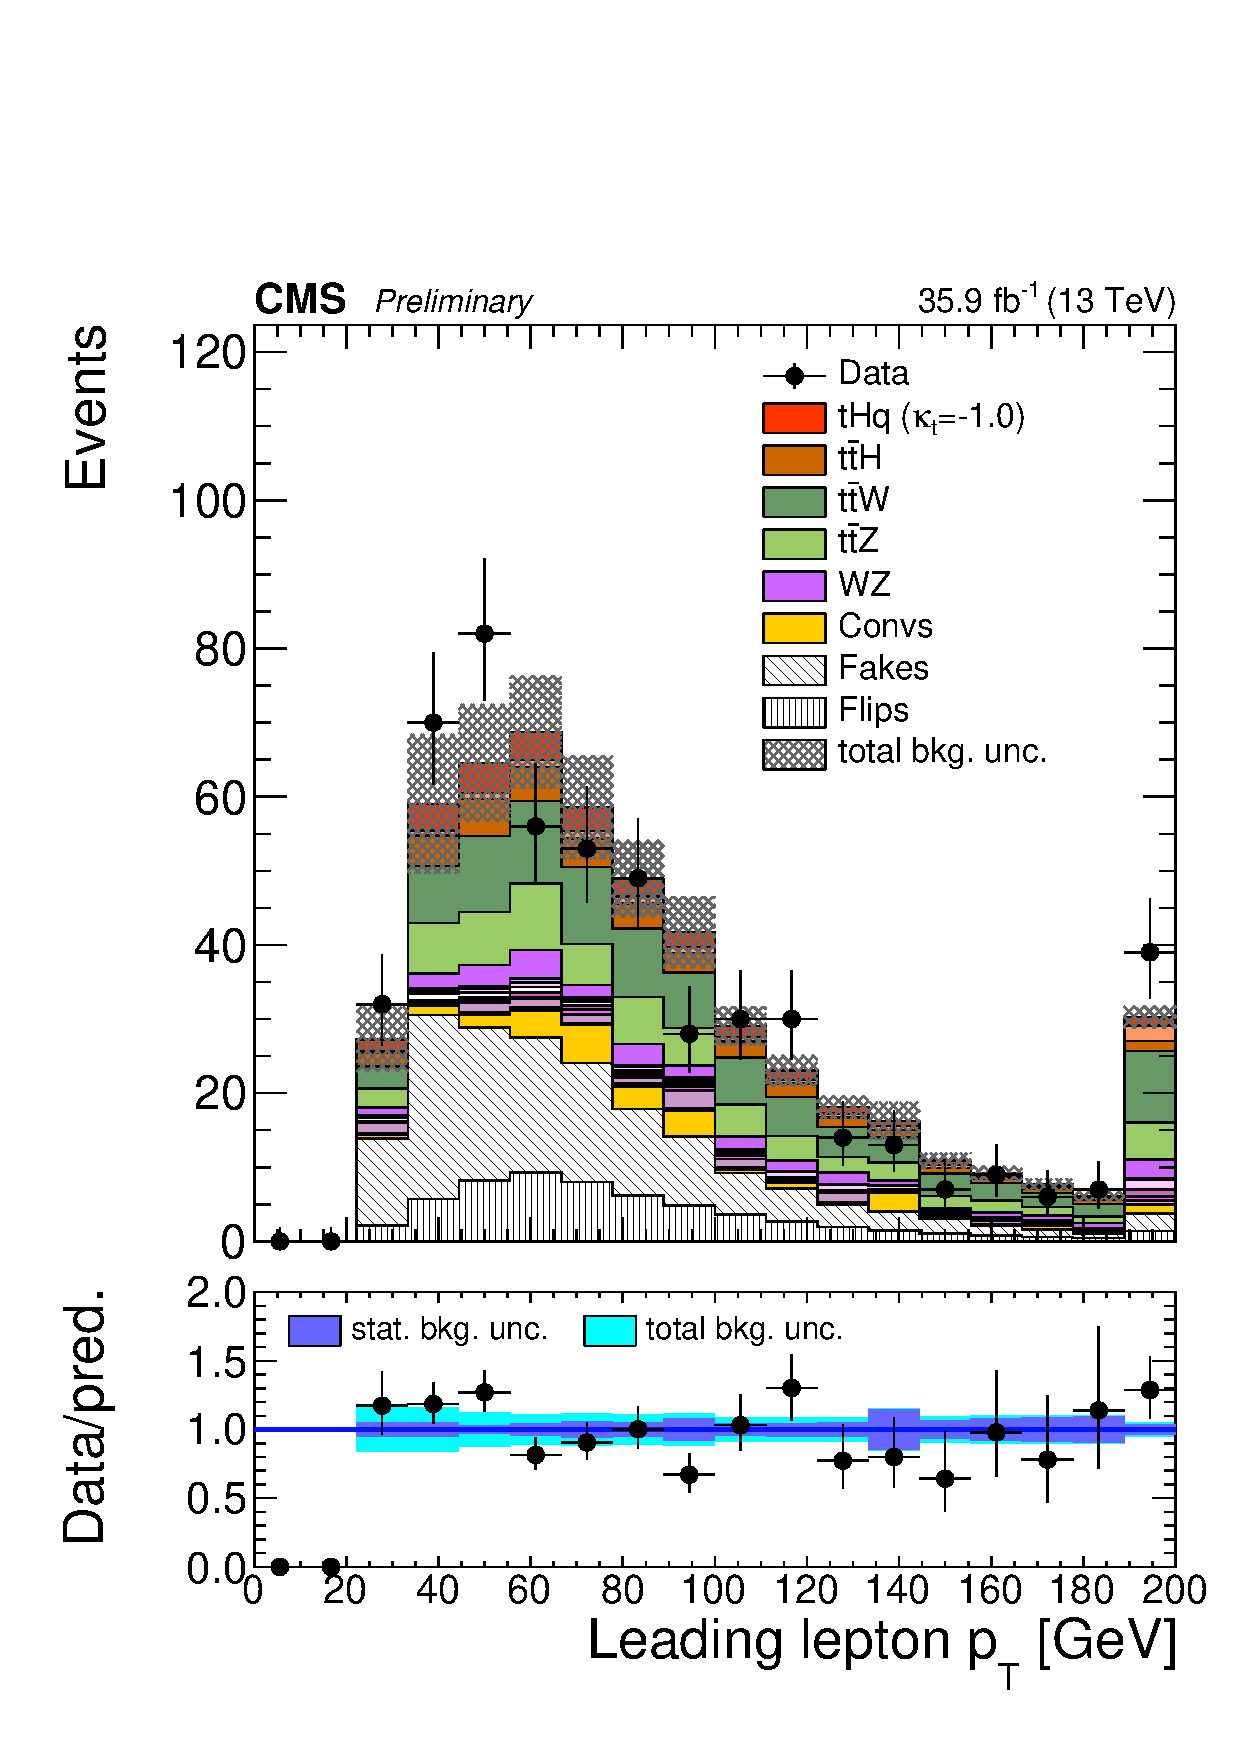
\includegraphics[width=0.32\textwidth]{controlplots/3l-Z/Lep1Pt.pdf}
        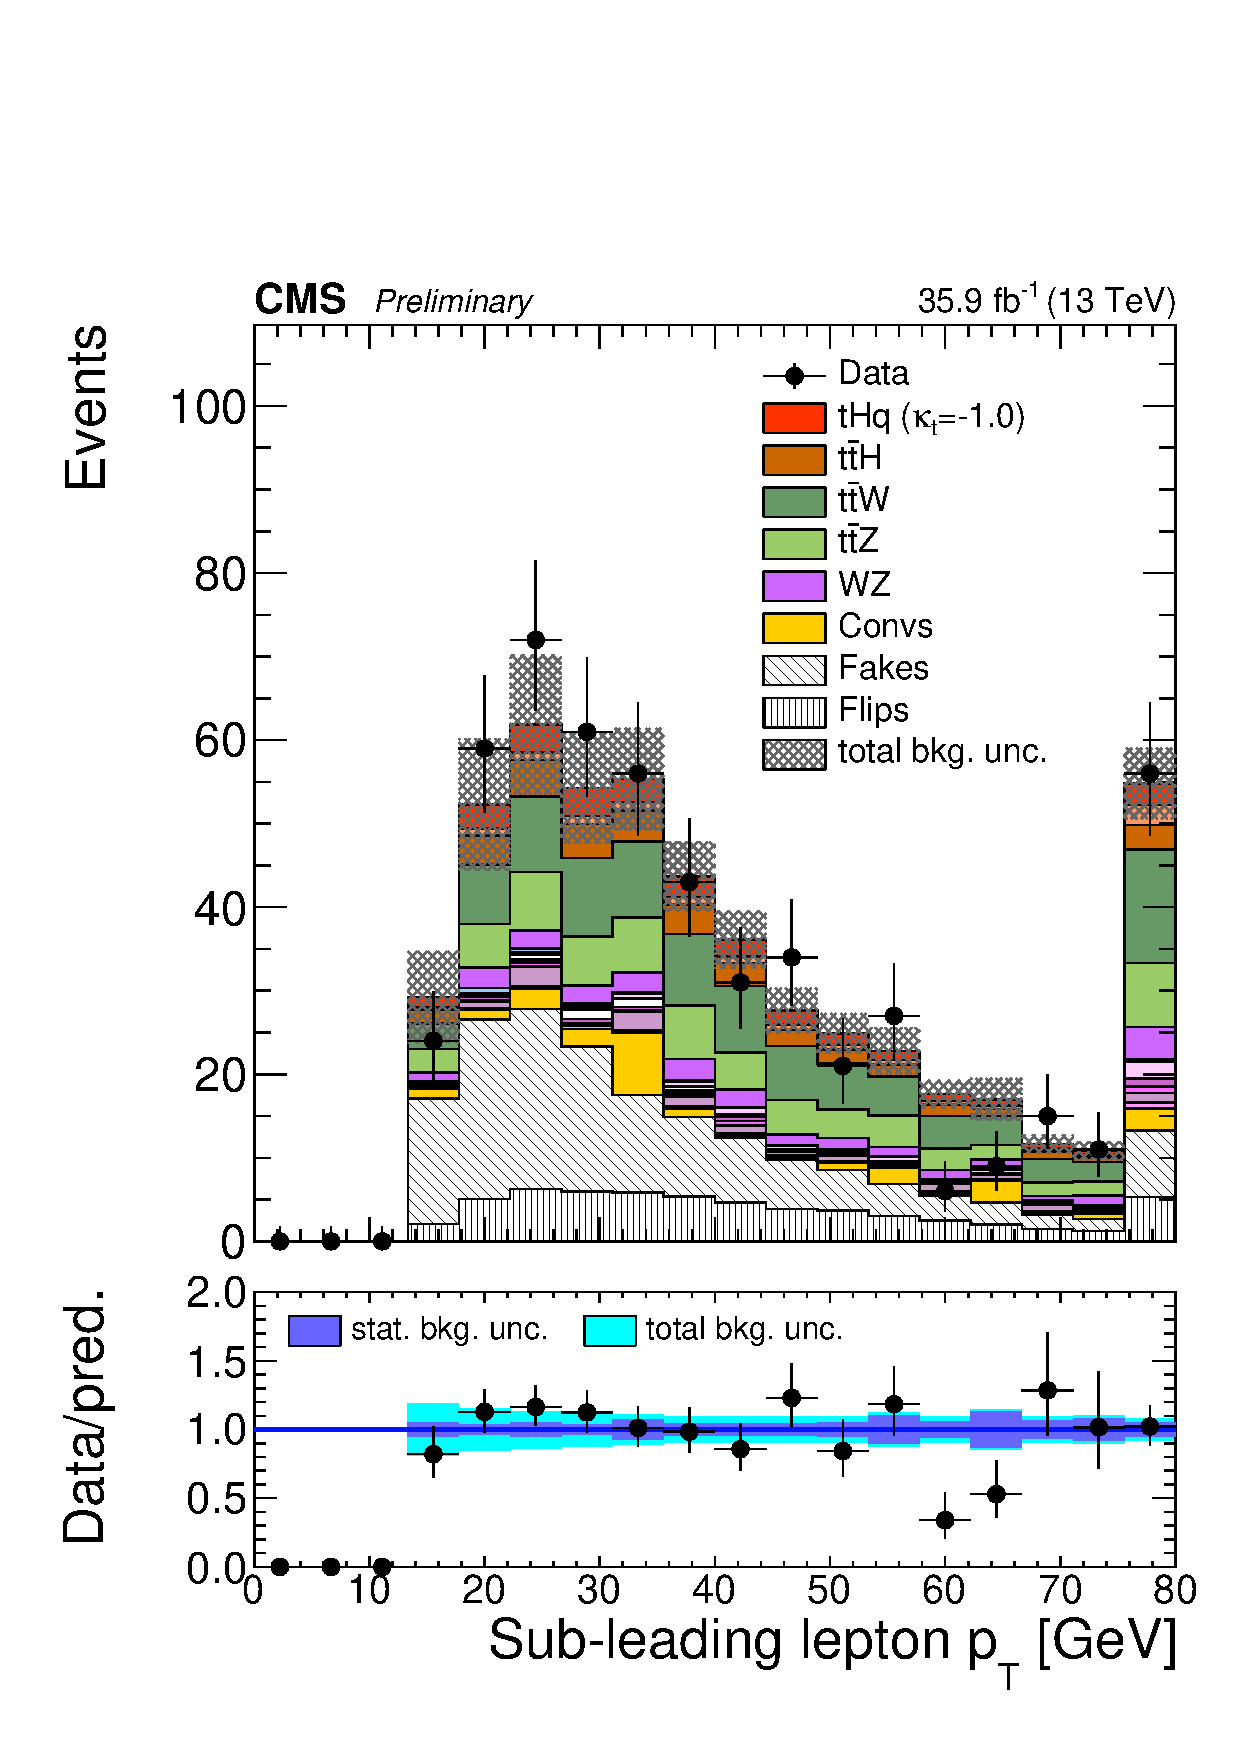
\includegraphics[width=0.32\textwidth]{controlplots/3l-Z/Lep2Pt.pdf}
        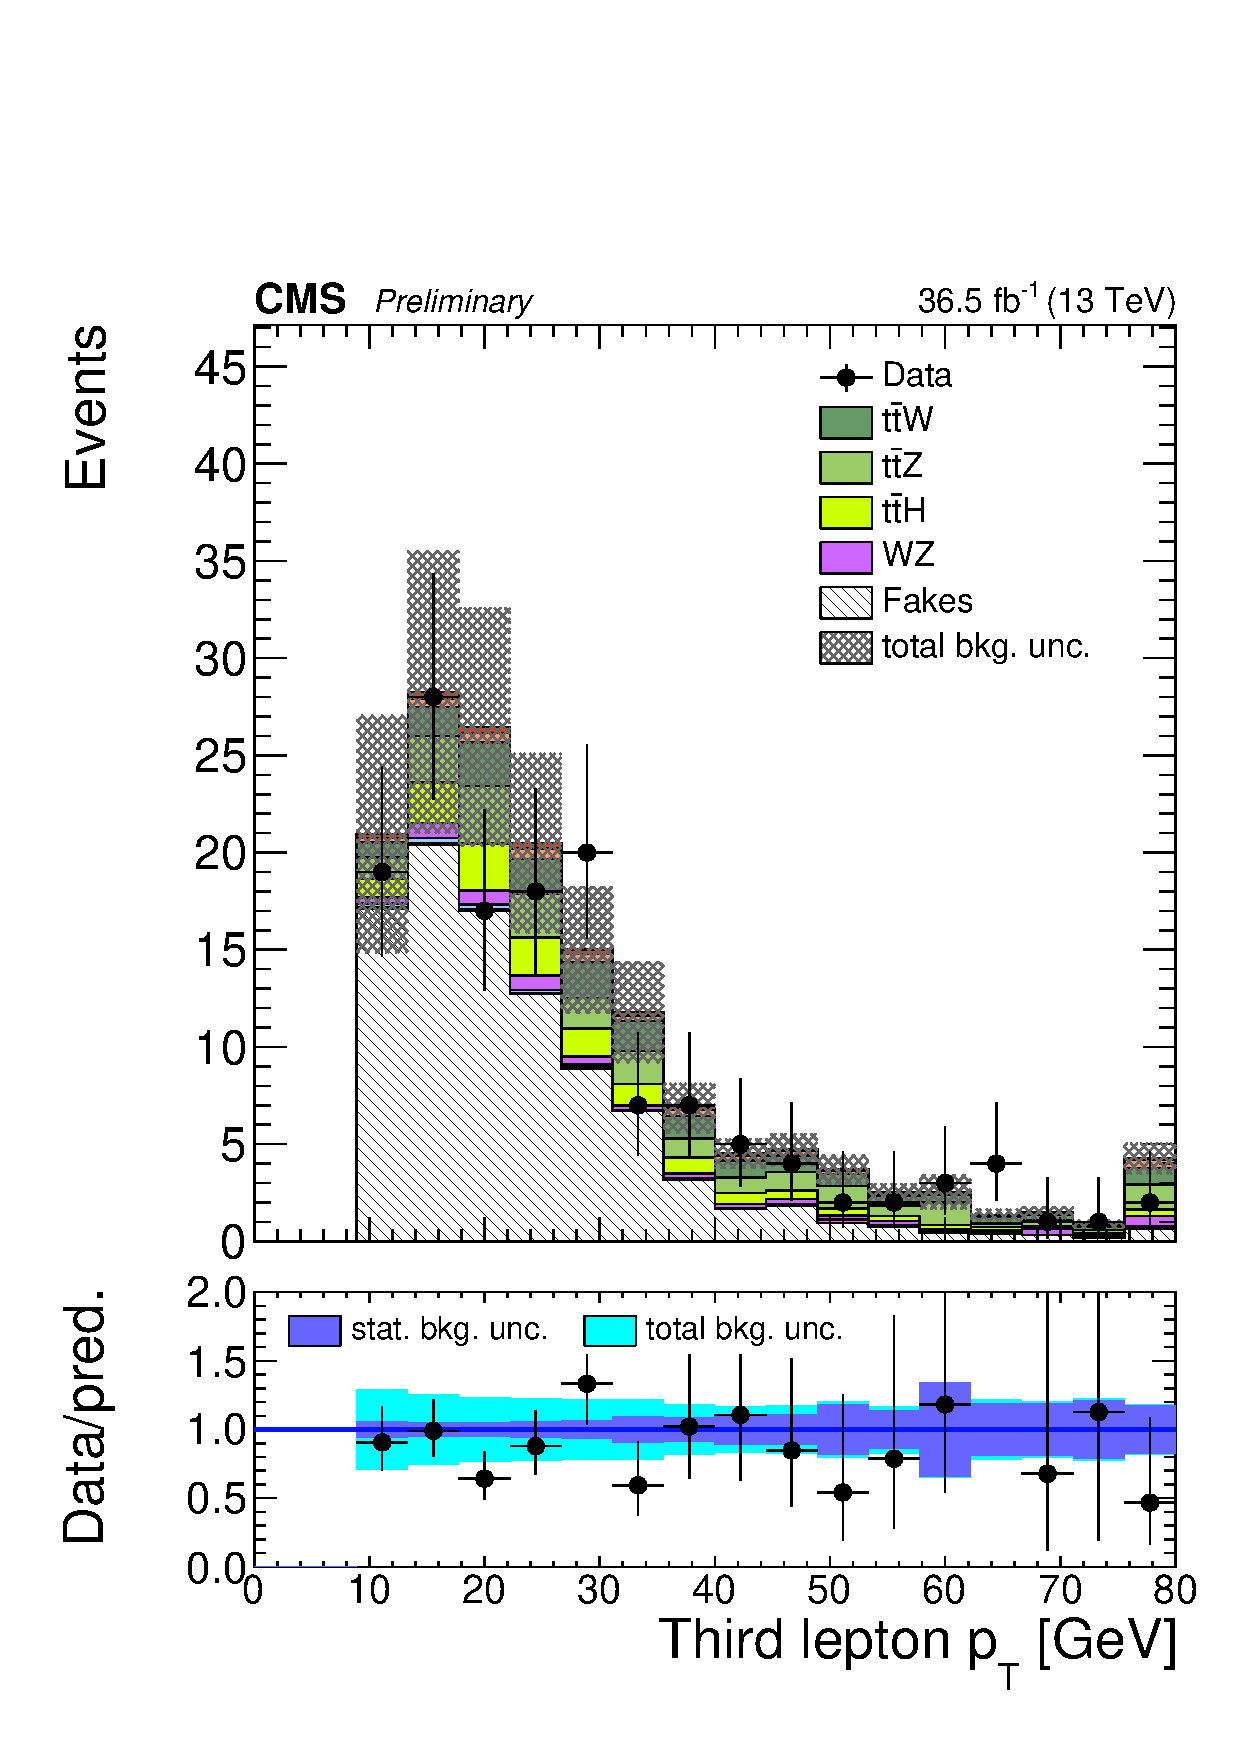
\includegraphics[width=0.32\textwidth]{controlplots/3l-Z/Lep3Pt.pdf} \\
        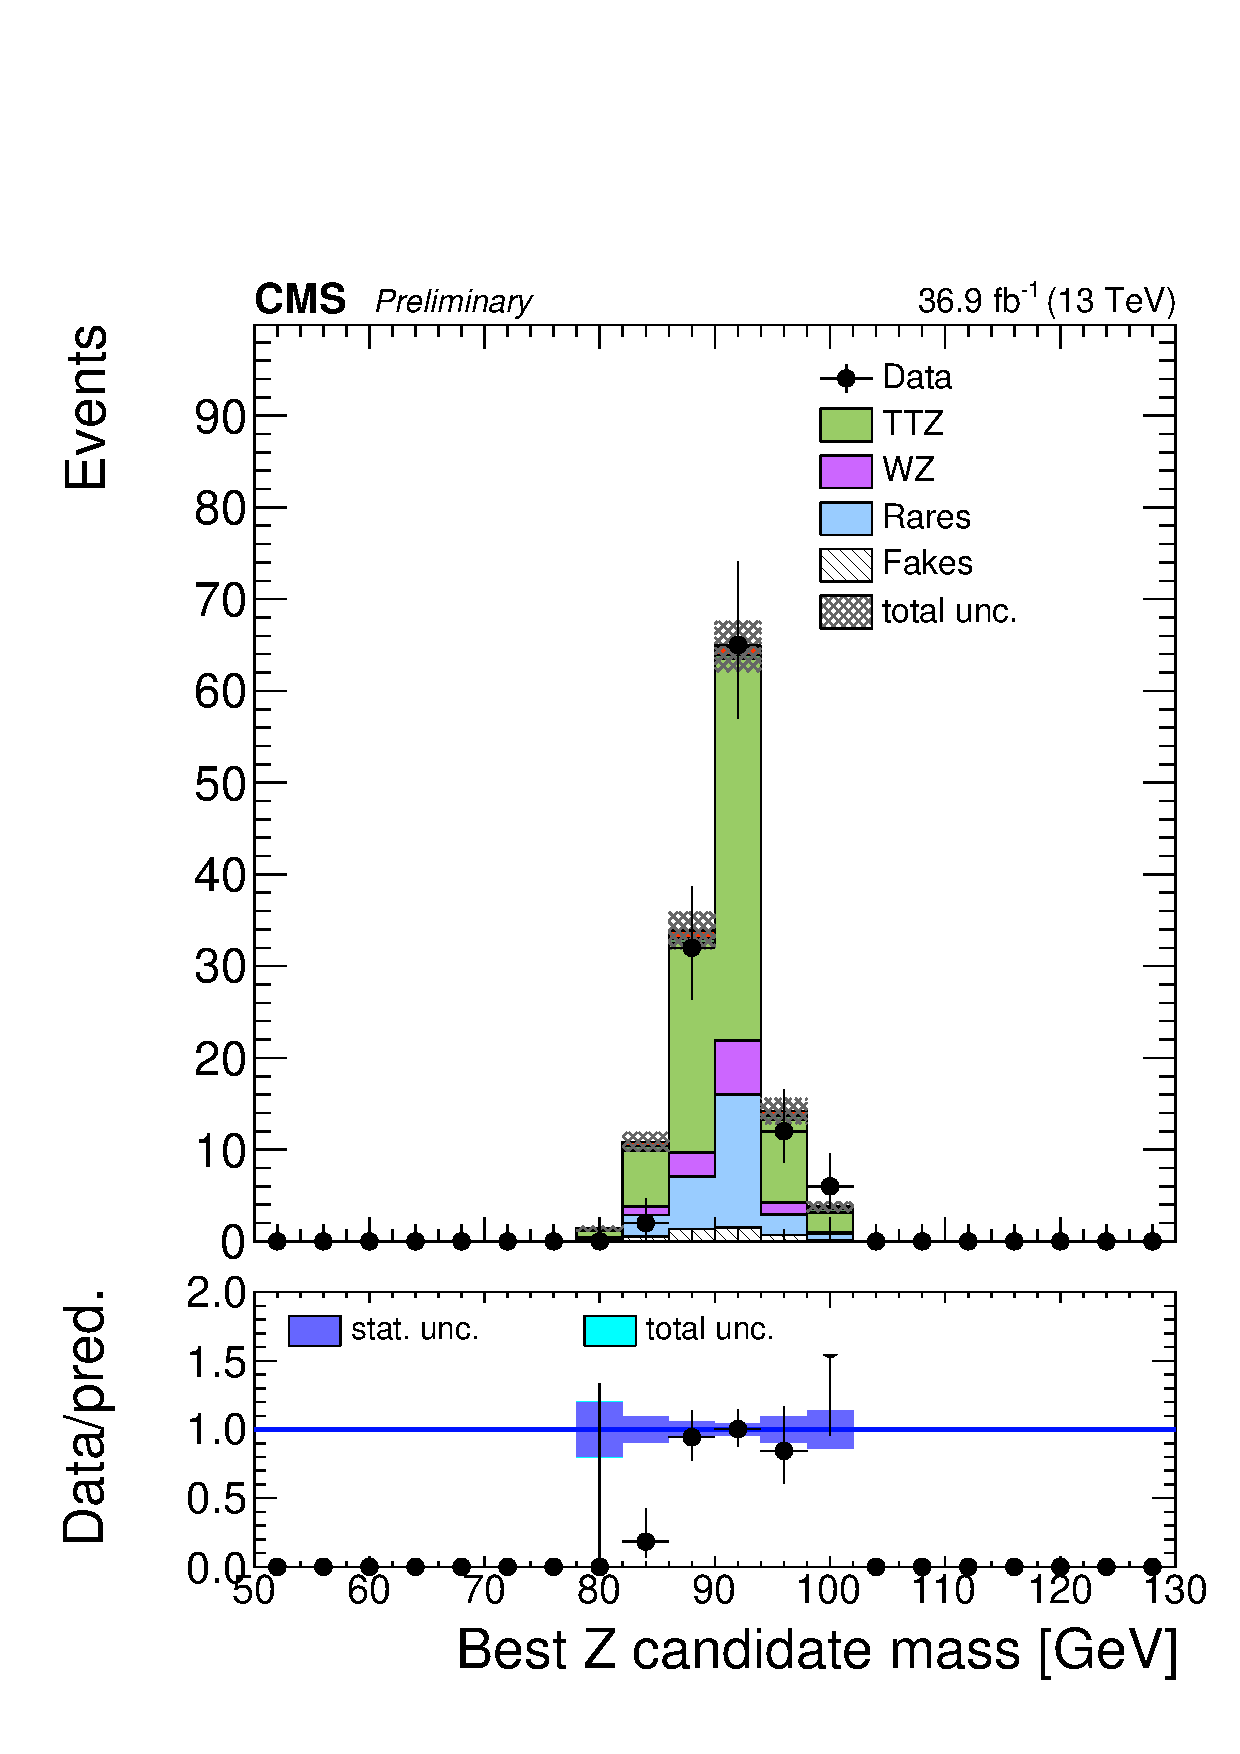
\includegraphics[width=0.32\textwidth]{controlplots/3l-Z/mZ1.pdf}
        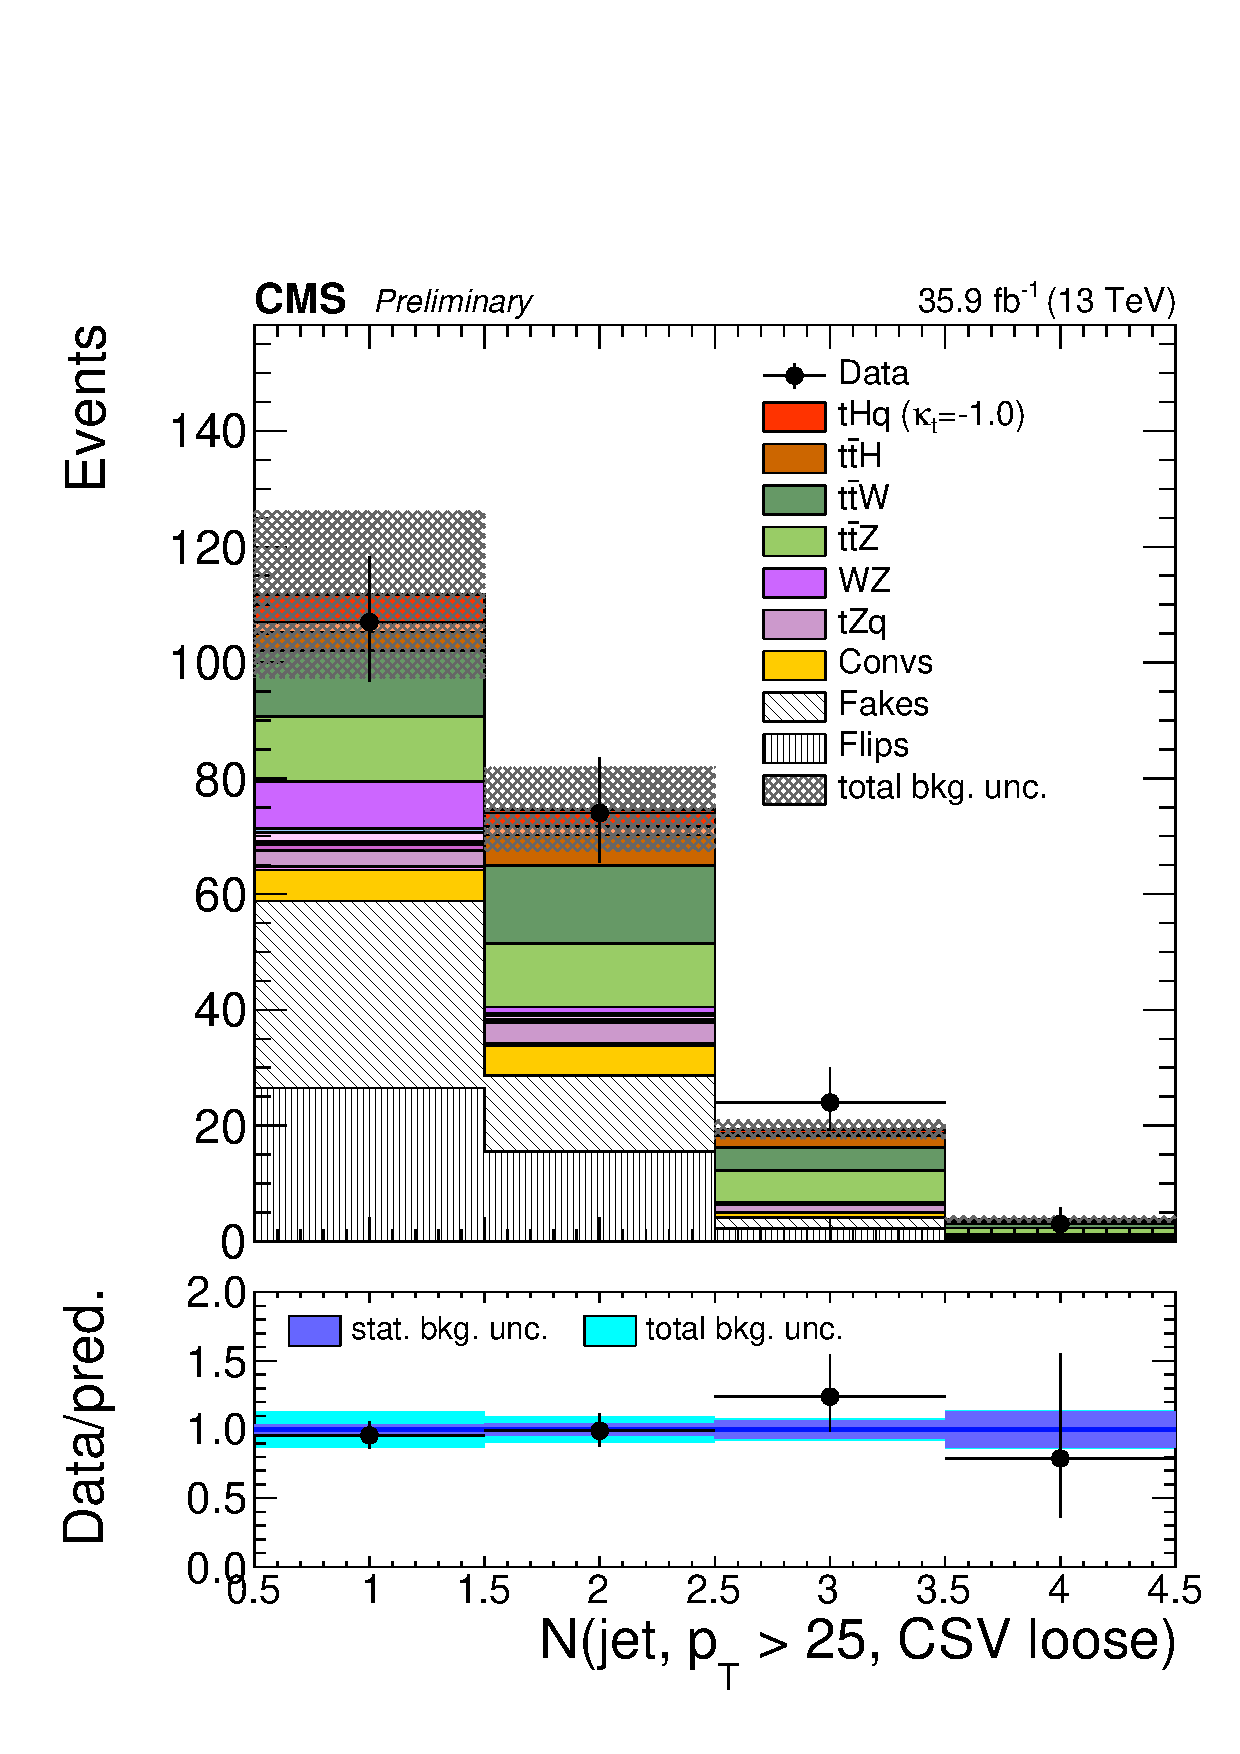
\includegraphics[width=0.32\textwidth]{controlplots/3l-Z/nBJetLoose25.pdf}
        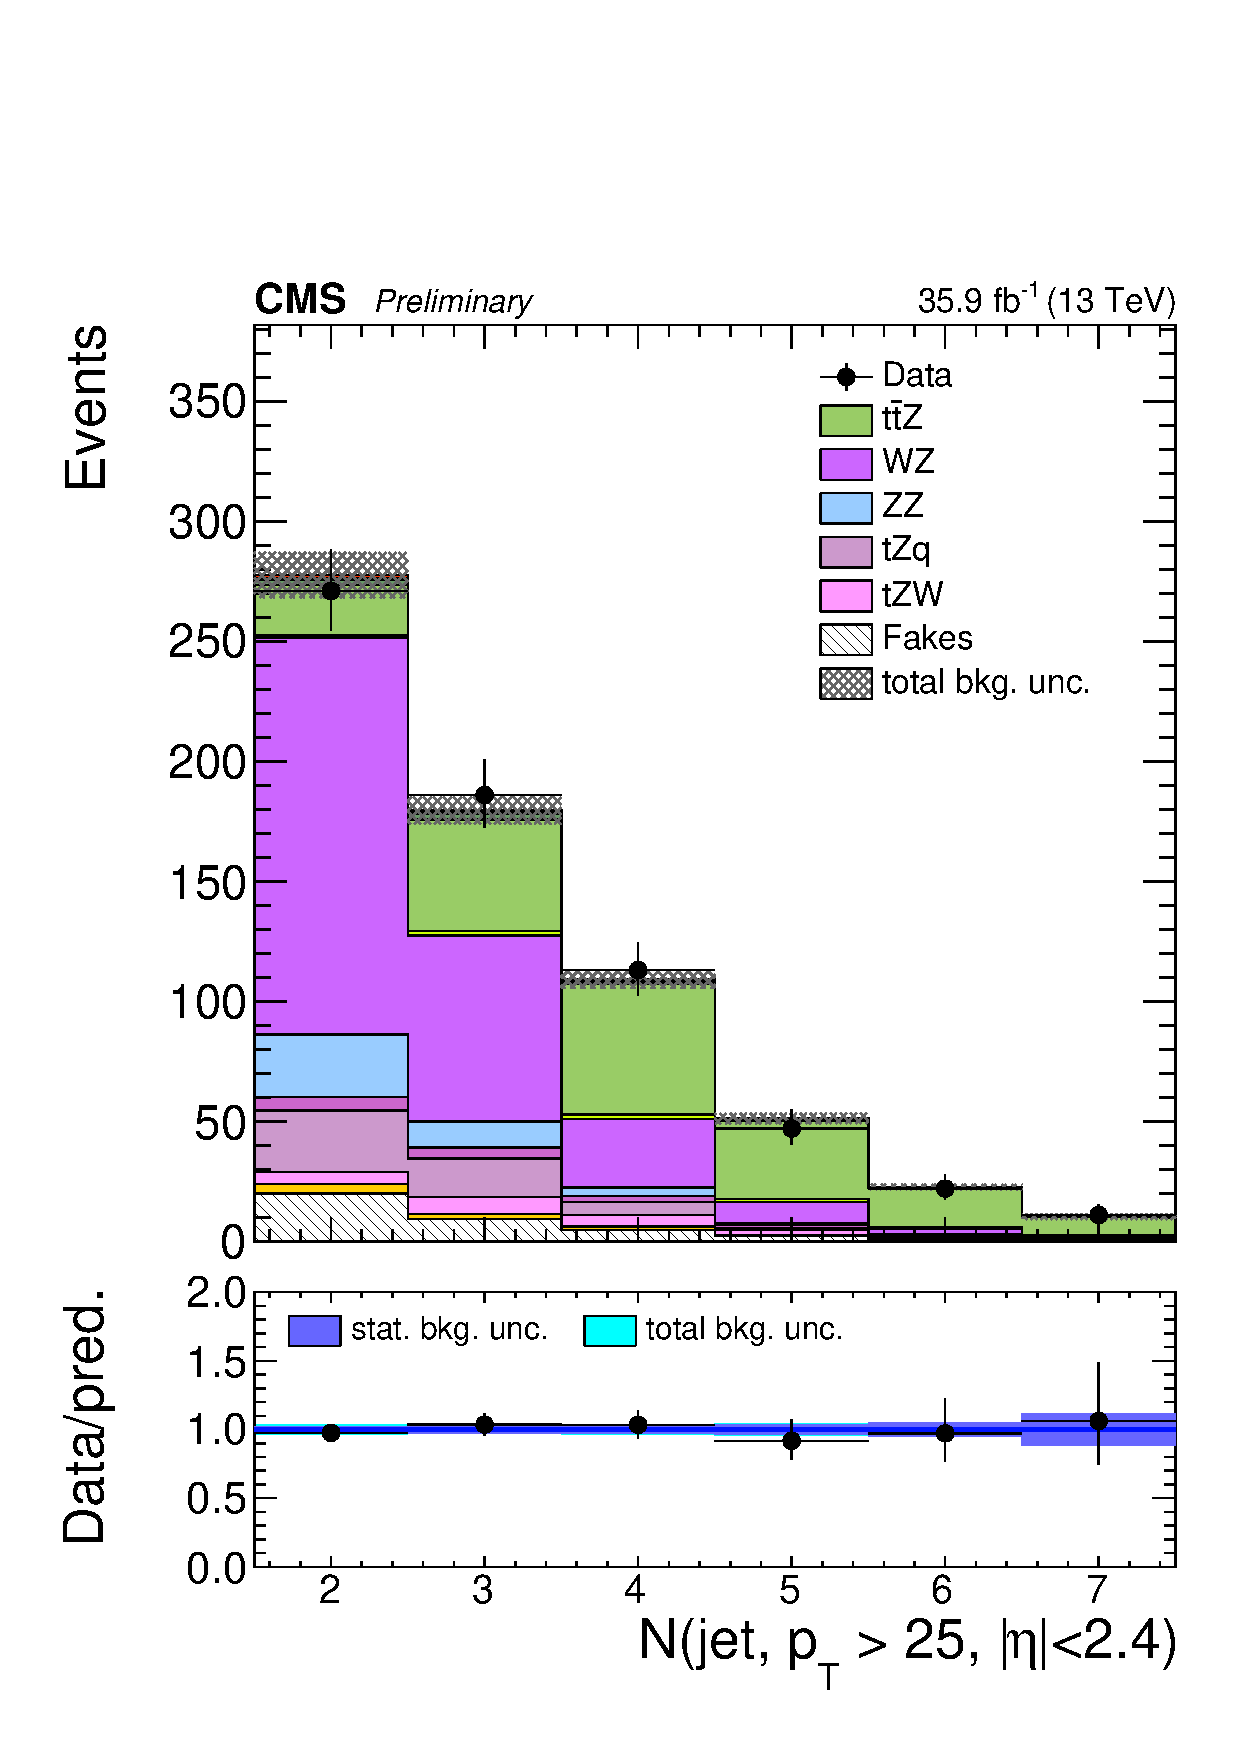
\includegraphics[width=0.32\textwidth]{controlplots/3l-Z/nJet25.pdf}
\caption{Kinematic distributions in the diboson control region.}
\label{fig:3lzcontrol}
\end{figure}
              
In order to test the usability of the diboson background scale factor in this analysis, a Z-enriched control region\footnote{This control region is different from the one used to find the scale factor.} was defined by inverting the Z-veto and requiring exactly three tight leptons with \pt > 25/15/15 GeV, one or more jets passing the CSVv2 loose working point and less than four central jets. Figure \ref{fig:3lzcontrol} shows the distribution of three variables in the diboson control region; the good agreement between MC and data motivates the adoption of the diboson background scale factor.

Most of the diboson events passing the signal selection contain jets from light quarks and gluons that are incorrectly tagged as $b$-jets; it makes the estimate mainly sensitive to the experimental uncertainty in the mis-tag rate rather than the theoretical uncertainty in the jet flavor composition. The overall uncertainty assigned to the diboson prediction is estimated from the statistical uncertainty due to the limited sample size in the control region (30\%), the residual background in the control region (20\%), the uncertainties on the $b$-tagging rate (10-40\%), and from the knowledge of PDFs and the theoretical uncertainties of the extrapolation (up to 10\%).

\subsection{Non-prompt and charge mis-ID backgrounds}\label{ssec:fake_rate}

The non-prompt lepton background contribution to the final selection is estimated using the fake factor method. The main idea of the method is to define a control region of events enriched in the background to estimate and determine a factor that relates (extrapolates) these events to those in the signal region. The method is data-driven in the sense that the control sample is selected from data, and the extrapolation factor is measured from data.

In the signal region of this analysis, non-prompt leptons are predominantly produced in \ttbar events, with a much smaller contribution from Drell-Yan production; therefore, the control region, also know as the \ti{application region}, is defined by modifying the event selection criteria in such a way that most of the events after selection are \ttbar events and thus the misidentification rate is increased; hence, in the application regions, the tight definition for electrons and muons are replaced by the the \ti{fakeable} object definitions in Tables ~\ref{tab:muonIDs} and~\ref{tab:eleIDs}. Since the fakeable definition is a loosened version of the tight definition, in the context of fake rates, the fakeable definition becomes the loose selection. 

The ratio between the number of events that pass both the loose and tight selections, and the number of events that pass the loose selection but fail the tight one, corresponds to the \ti{loose-to-tight ratio or fake factor/rate (f)}. The measurement of the fake factor is made using two background dominated data samples, collected with dedicated triggers, %(subtracting the residual prompt lepton contribution using MC)
as a function of \pt and |$\eta$| and separately for muons and electrons:

\begin{itemize}
\item A sample dominated by QCD multijet events, collected using single lepton triggers at relatively high \pt thresholds. It is used to extract ratios for lepton candidates with \pt above 30 GeV.
\item A sample dominated by Z + jets events, where the two high-\pt leptons resulting from the Z decay are used to trigger the events without biasing the \pt spectrum of a third lepton at low transverse momentum. It is used to determine the ratios for low-\pt leptons. 
\end{itemize}

Processes like $W$ + jets, $Z$ + jets , \WZ and \ZZ produce prompt leptons that contaminate the samples; thus, they are suppressed by vetoing additional leptons in the selection, and the residual contamination is then subtracted using the transverse mass as a discriminating variable.

The extrapolation from the application region to the signal region is performed by weighting the events in the application region using the fake factor according to the following rules:

\begin{itemize}
\item events with one lepton failing the tight criteria are weighted with the factor $\frac{f}{(1-f)}$ for the estimate to the signal region. 
\item events with two leptons (i,j) failing the tight criteria are weighted with the factor $-\frac{f_if_j}{(1-f_i)(1-f_j)}$ for the estimate to the signal region. 
\item events with three leptons (i,j,k) failing the tight criteria are weighted with the factor $\frac{f_if_jf_k}{(1-f_i)(1-f_j)(1-f_k)}$ for the estimate to the signal region. 
\end{itemize}

\begin{figure}[htb]
\centering
        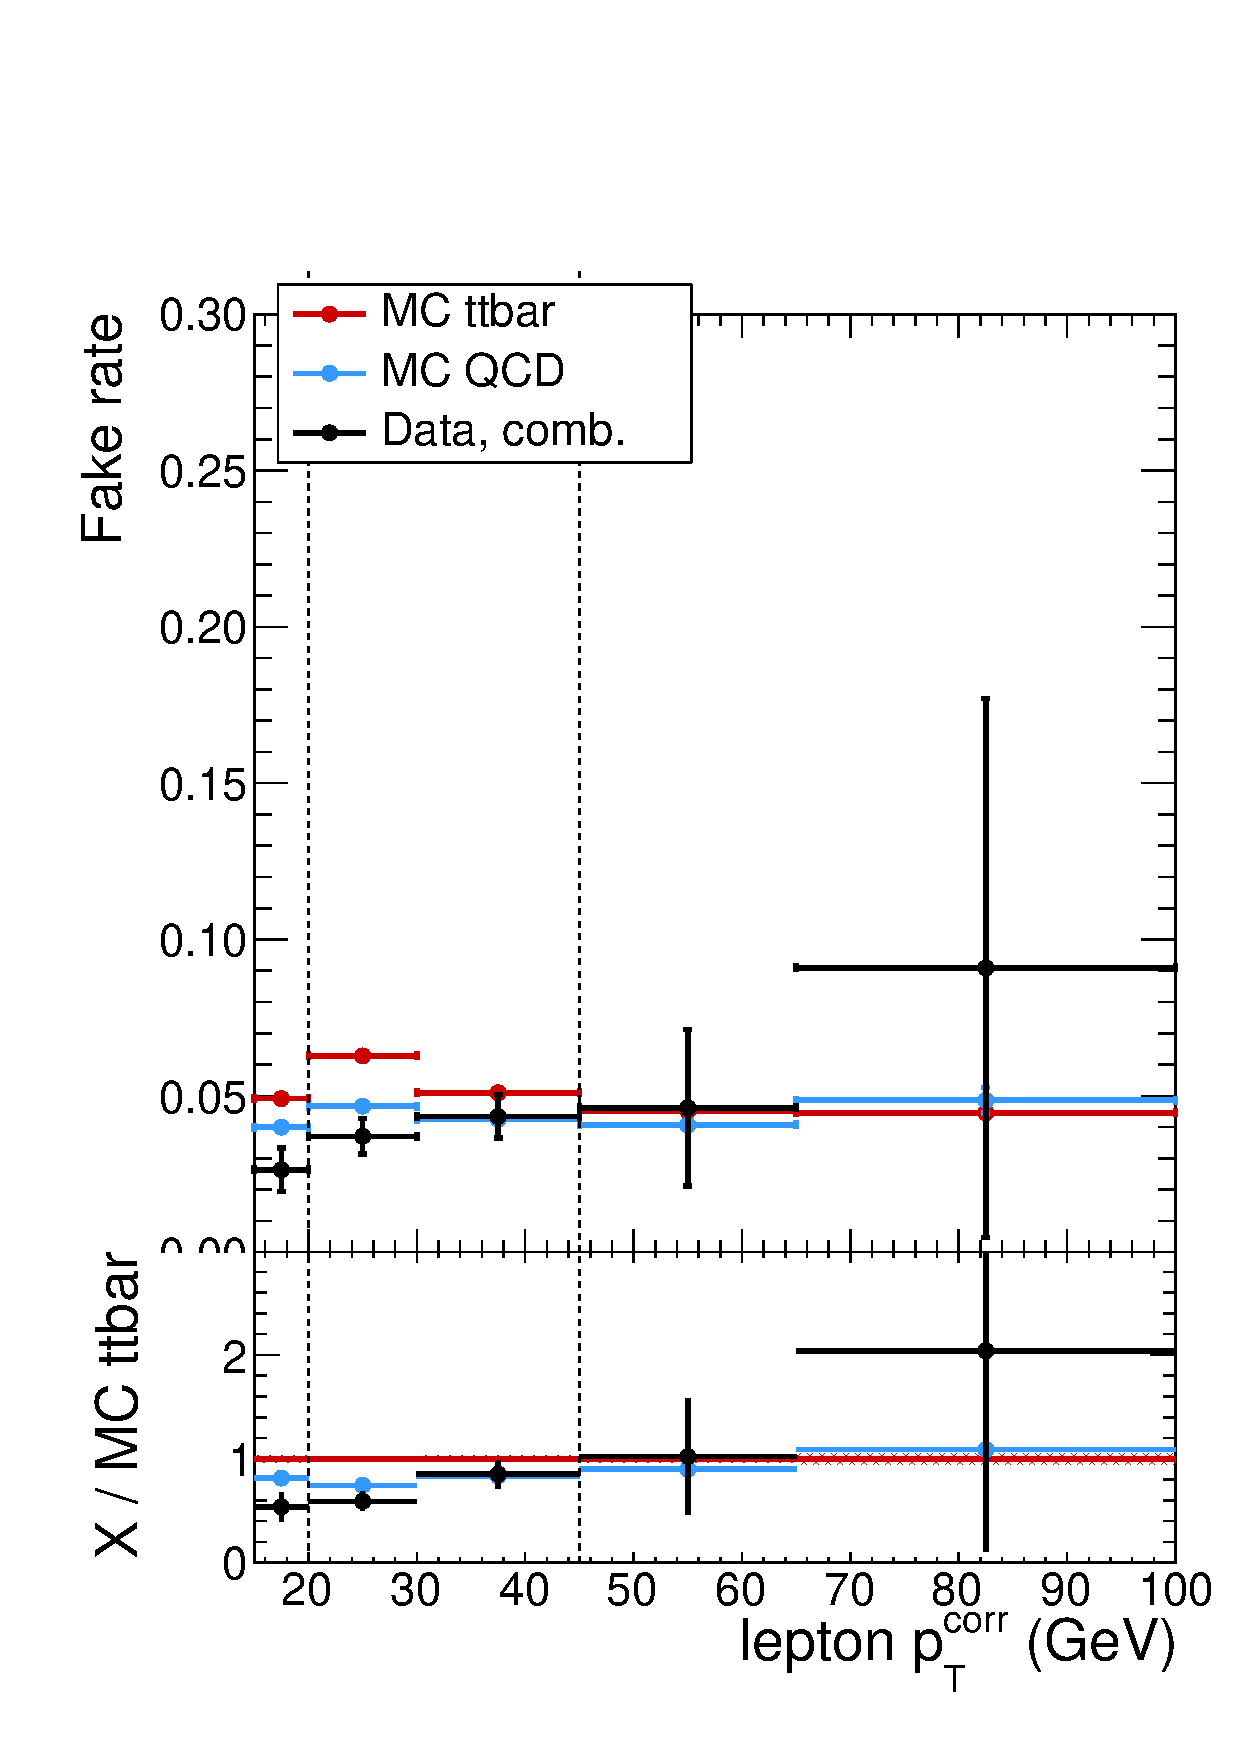
\includegraphics[width=0.33\textwidth]{fr_mu_barrel}
        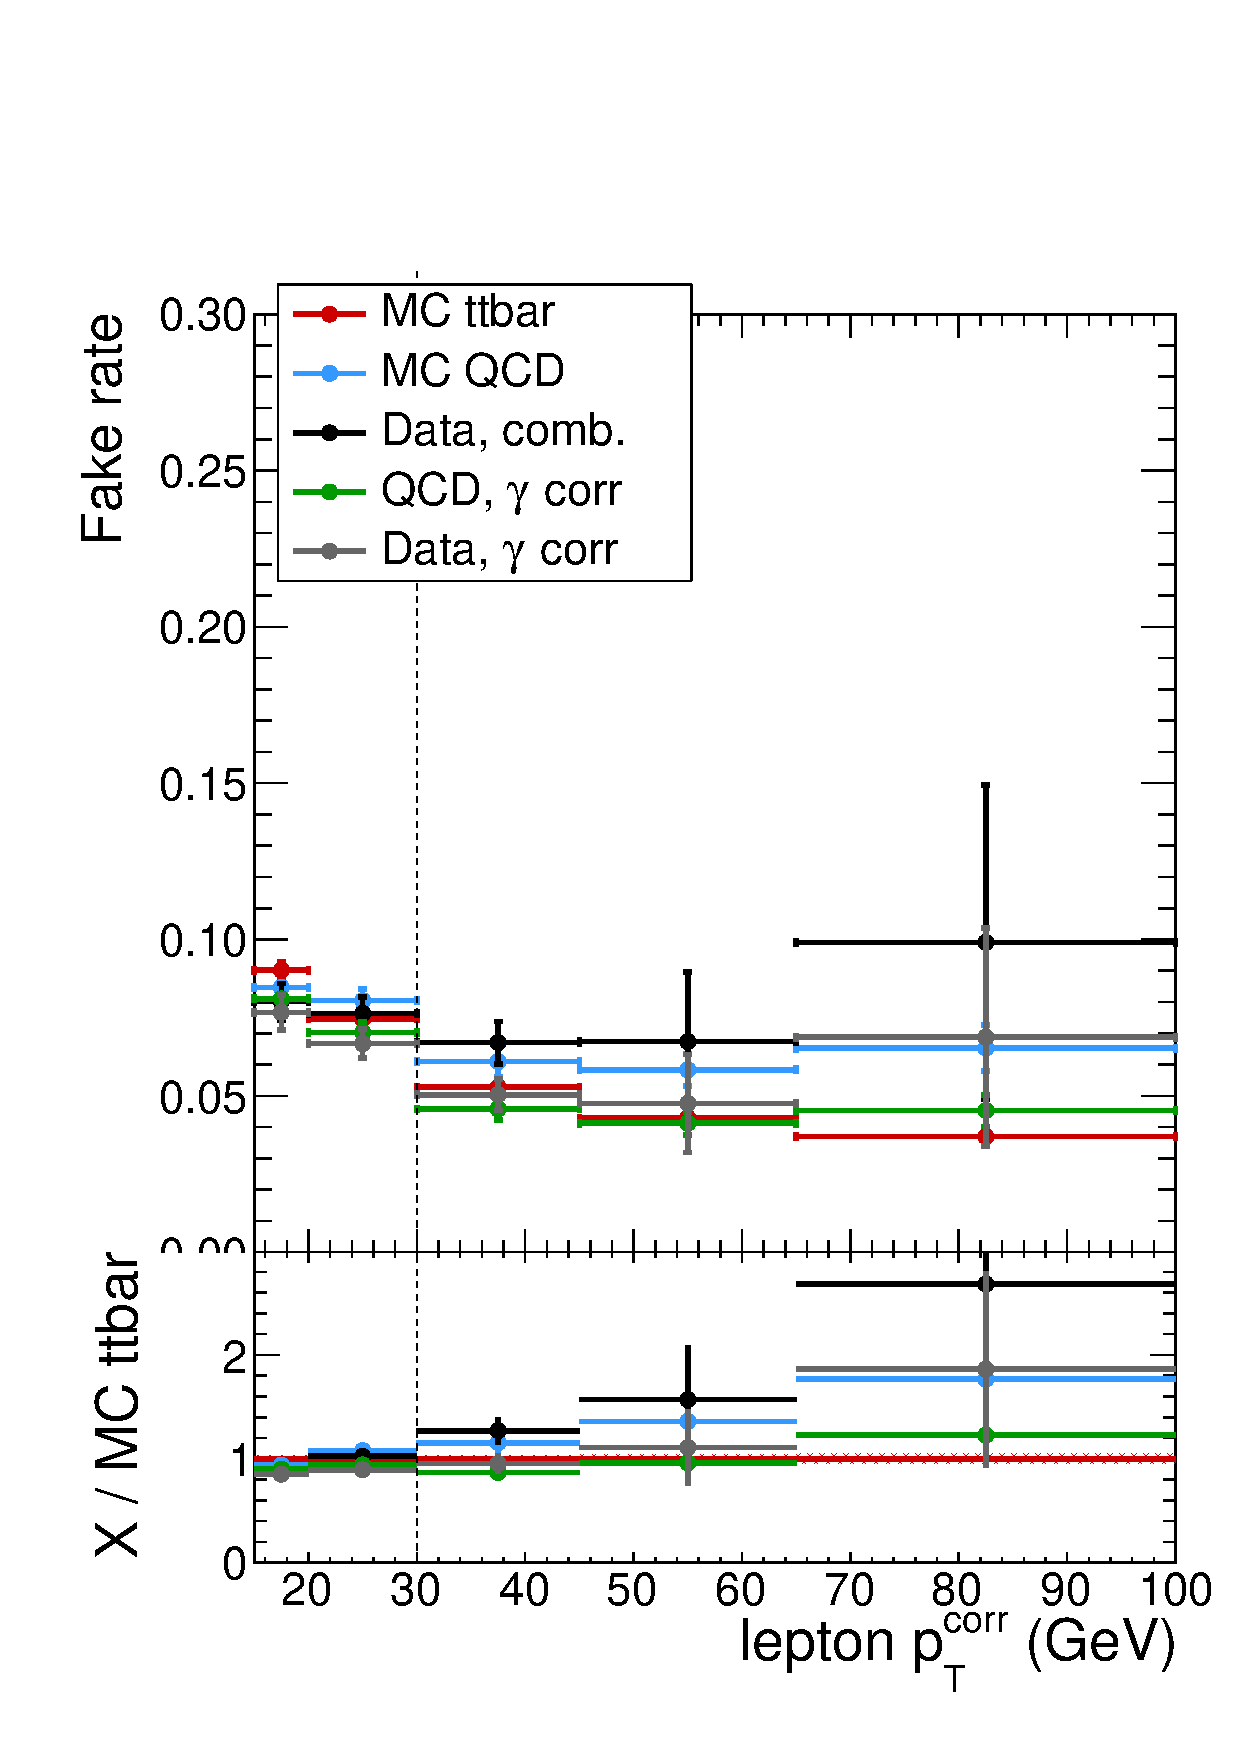
\includegraphics[width=0.33\textwidth]{fr_el_barrel} \\
        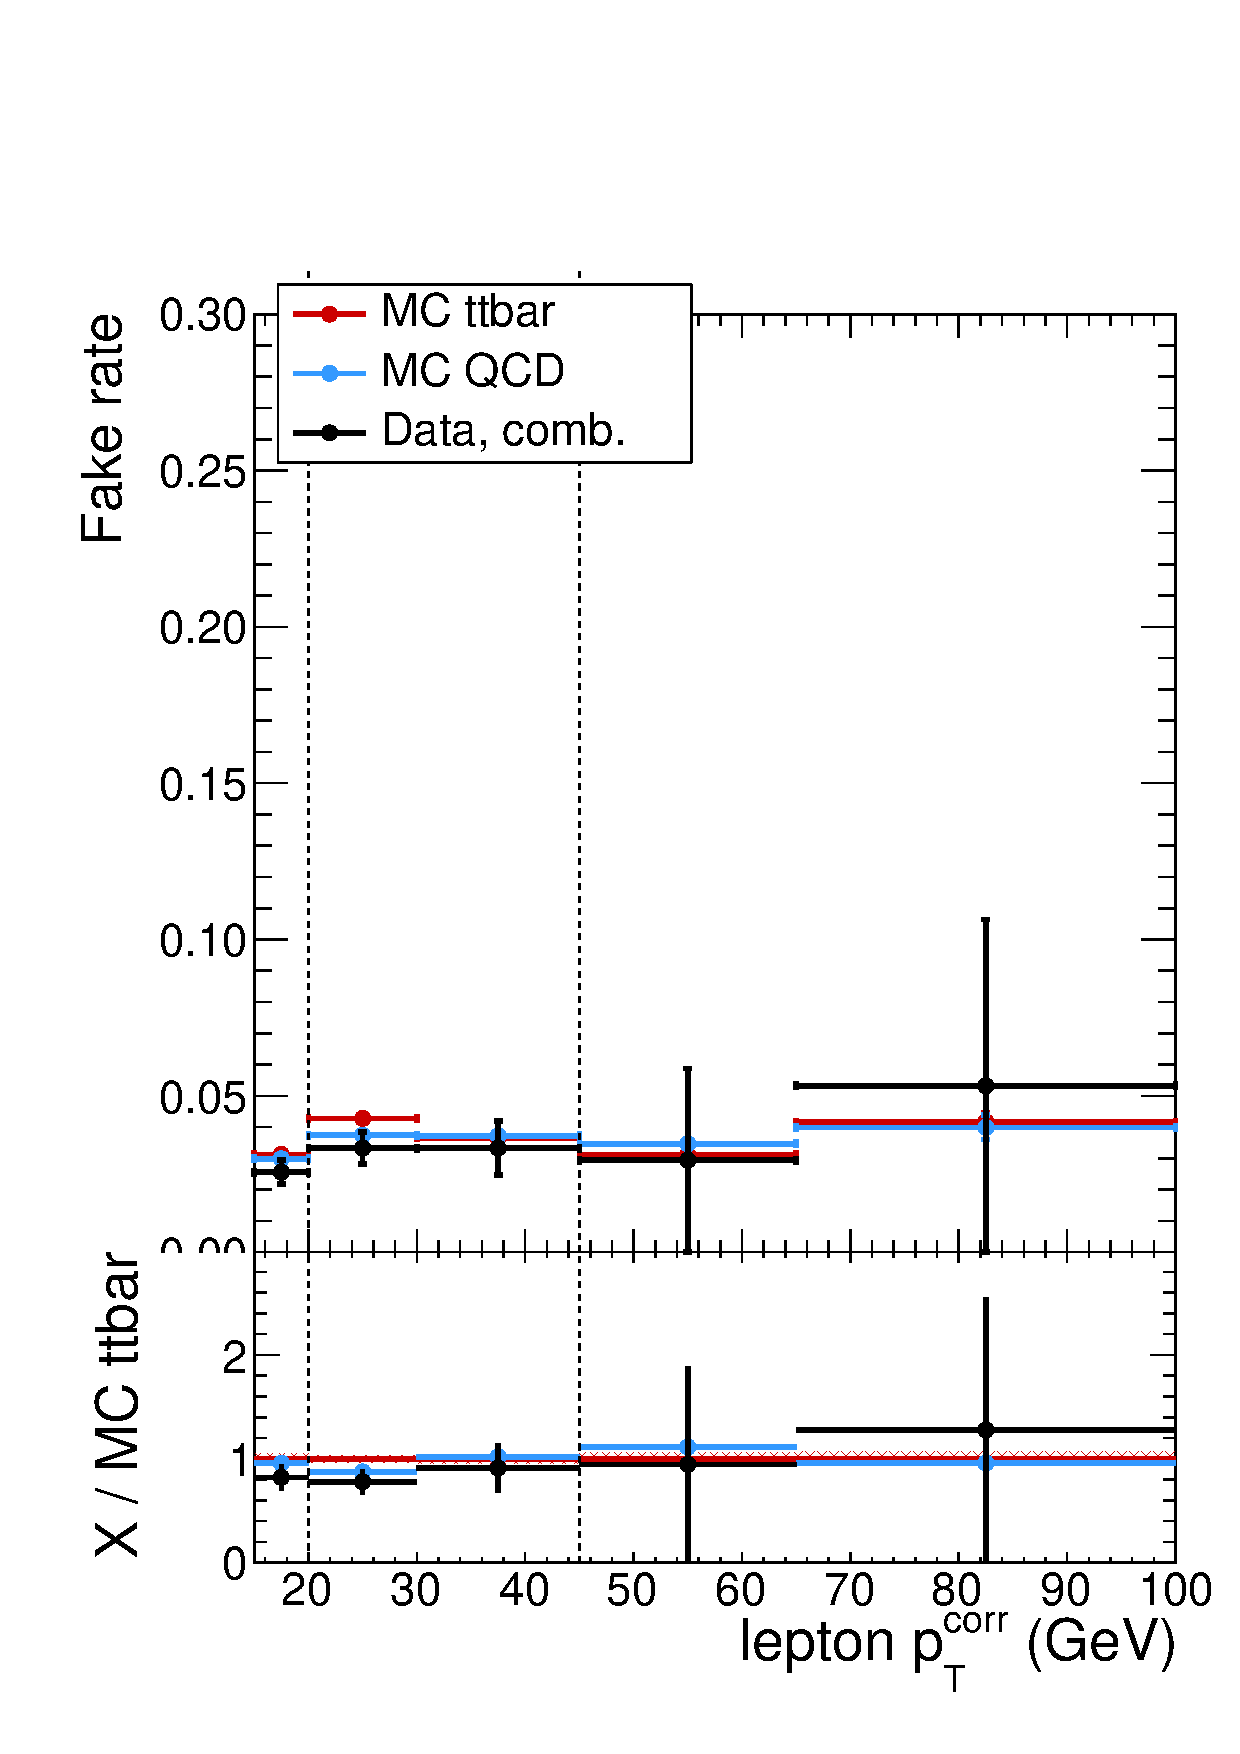
\includegraphics[width=0.33\textwidth]{fr_mu_endcap}
        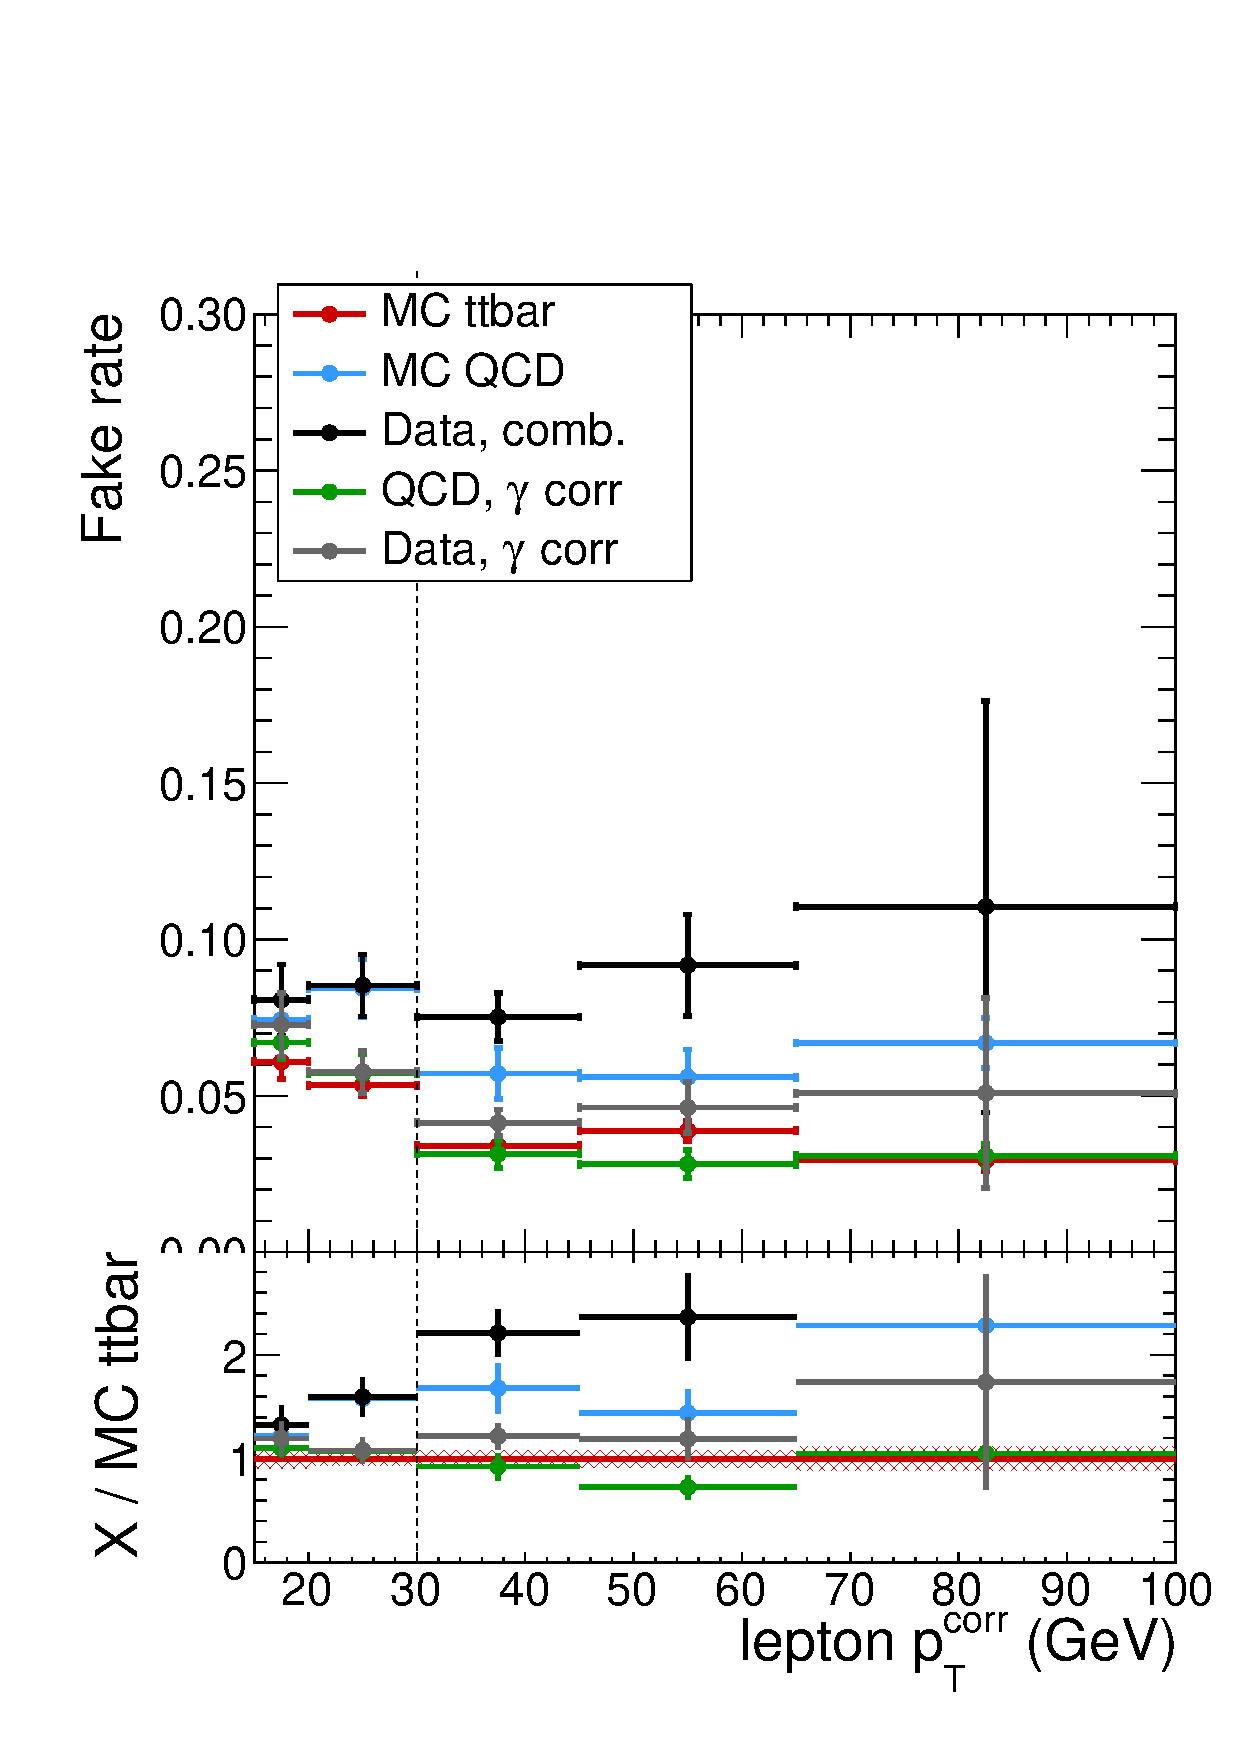
\includegraphics[width=0.33\textwidth]{fr_el_endcap}
\caption[Fake rates]{Fake rate measurement in events in data for muons (left column) and electrons (right column). Predictions from simulated events in the measurement region (blue) and from non-prompt leptons in \ttbar (red) are included for comparison. Top row is for ${|\etac|<2.5}$ and bottom row for |$\etac$|>2.5.}
\label{fig:frmeas-comb-data}
\end{figure}

Figure \ref{fig:frmeas-comb-data} shows the fake rates for electrons and muons used in this analysis which were taken from the studies in Reference \cite{CMS_AN_2017-029}.

The resulting prediction of the event yield in the signal selection carries an uncertainty of 30-50\% which is composed of the statistical uncertainty in the measurement of the fake rates due to prescaling of lepton triggers, the uncertainty in the subtraction of residual prompt leptons from the control region, and from testing the closure of the method in simulated background events; hence, it is one of the dominant limitations on the performance of multilepton analyses in general and this analysis in particular.

Finally, an additional source of background arises in the $2lss$ channel from events with an originally opposite-sign lepton pair for which the charge of one of the leptons is misidentified (\ti{charge mis-ID}); usually this happens because of the conversion of hard bremsstrahlung photons emitted from the initial lepton, hence, it is more likely to happen for electrons than for muons.

The charge mis-ID background is estimated from the yield of opposite-sign events in the signal region by measuring the charge mis-ID probability in same-sign and opposite-sign events compatible with a Z boson decay, in several bins of \pt\ and \etac, and weighting events with opposite-sign leptons in the signal selection.

\begin{table}[htp]
\centering
\begin{tabular}{lccc}\hline
 Data                & $10\leq\pt<25$ GeV  & $25\leq\pt<50$ GeV  & 50 GeV$\leq\pt$ \\\hline
$0\leq\eta<1.48$     & 0.0442 $\pm$ 0.0011 & 0.0179 $\pm$ 0.0004 & 0.0262 $\pm$ 0.0020 \\
$1.48\leq\eta<2.5$   & 0.1329 $\pm$ 0.0066 & 0.1898 $\pm$ 0.0014 & 0.3067 $\pm$ 0.0113 \\\hline
 MC                  &                     &                     &                      \\\hline
$0\leq\eta<1.48$     & 0.0378 $\pm$ 0.0016 & 0.0222 $\pm$ 0.0003 & 0.0233 $\pm$ 0.0015 \\
$1.48\leq\eta<2.5$   & 0.0956 $\pm$ 0.0044 & 0.2108 $\pm$ 0.0027 & 0.3157 $\pm$ 0.0018 \\\hline
\end{tabular}
\caption[Electron charge mis-ID probabilities.]{Electron charge mis-ID probabilities (in percent), determined in data (top) and Drell-Yan MC (bottom)\cite{CMS_AN_2017-029}.}
\label{tab:chmisid_prob}
\end{table}

The charge mis-ID probability is found to be negligible for this analysis for muons, whereas for
electrons it ranges from about 0.02\% in the barrel section (|\etac| < 1.48) up to about 0.35\% in the detector endcaps (1.48 < |\etac| < 2.5), as shown in Table \ref{tab:chmisid_prob} and Figure \ref{fig:chmisid_prob}.

\begin{figure}[htp]
\centering
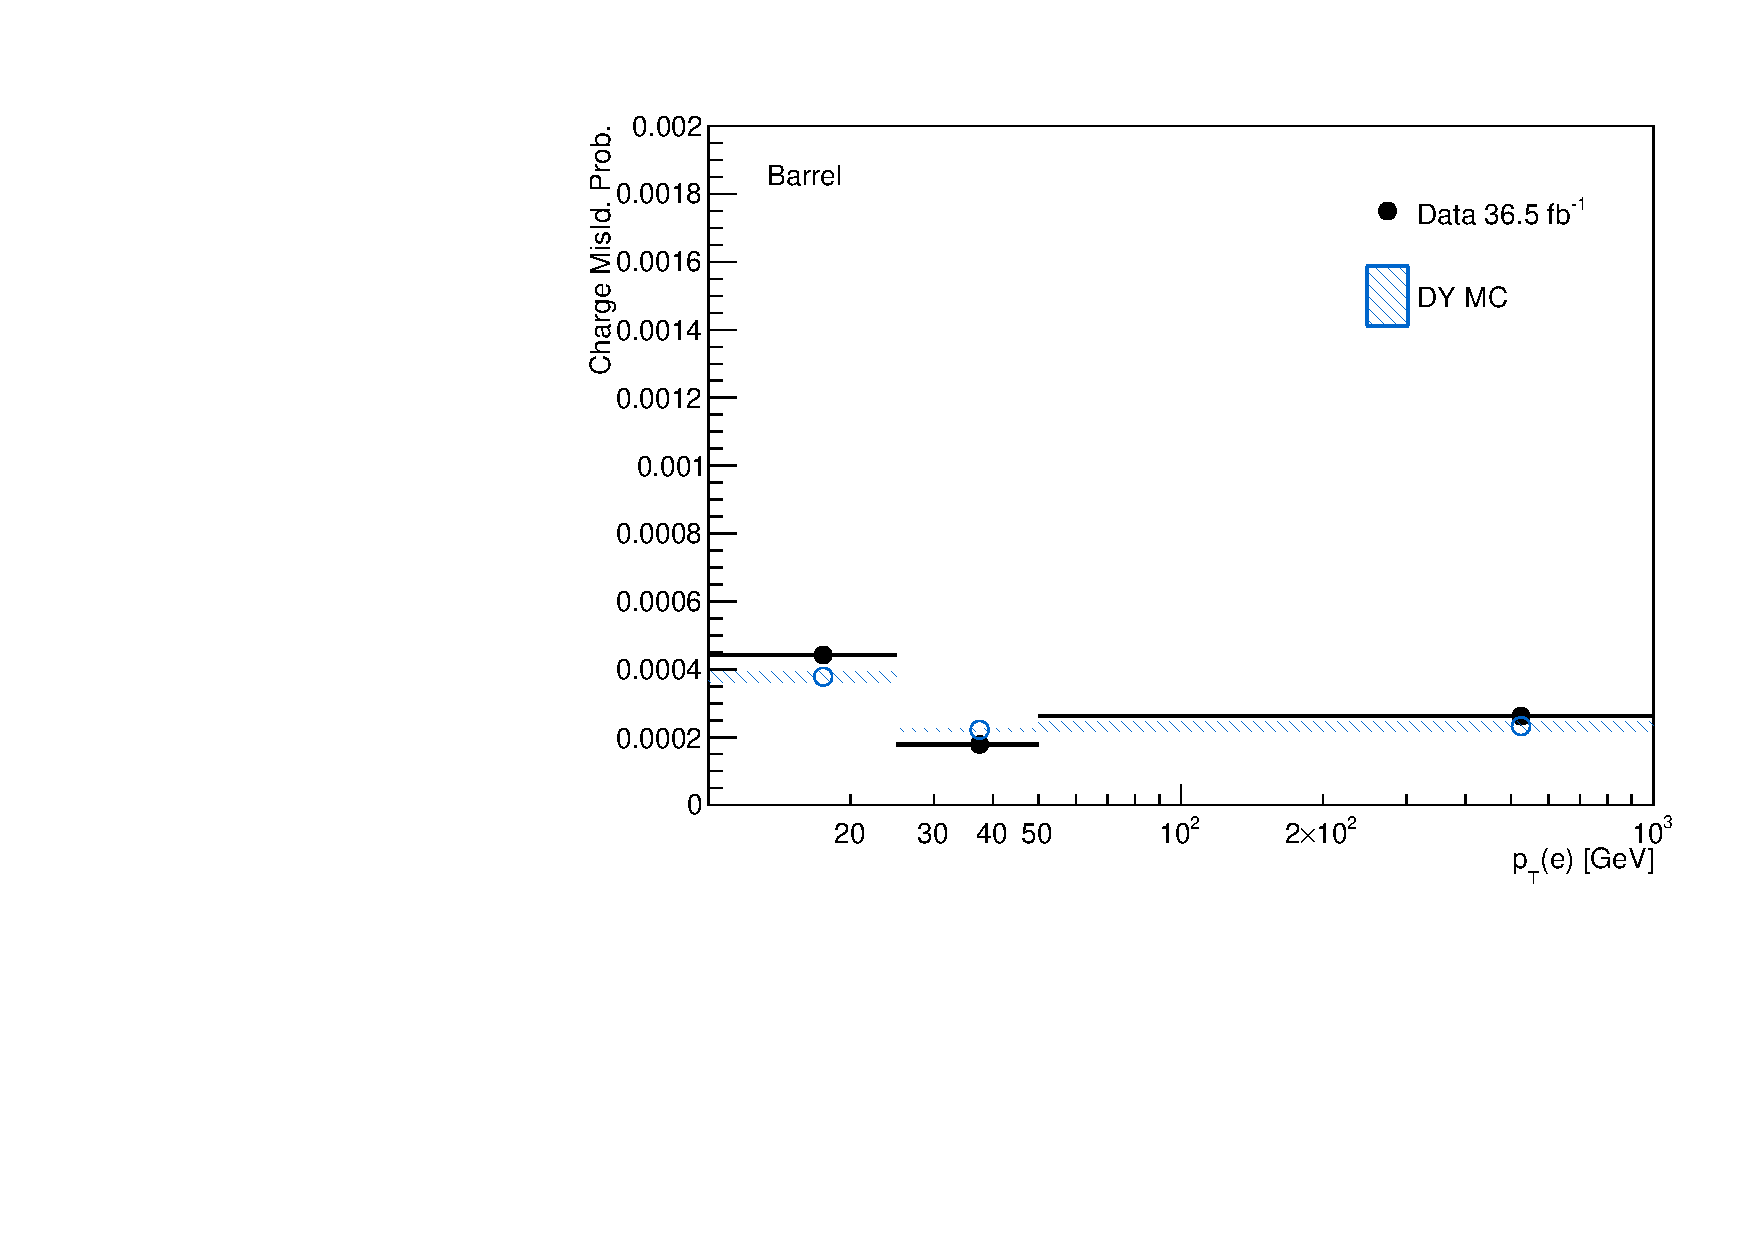
\includegraphics[width=0.49\textwidth]{chmid_prob_barrel.pdf}
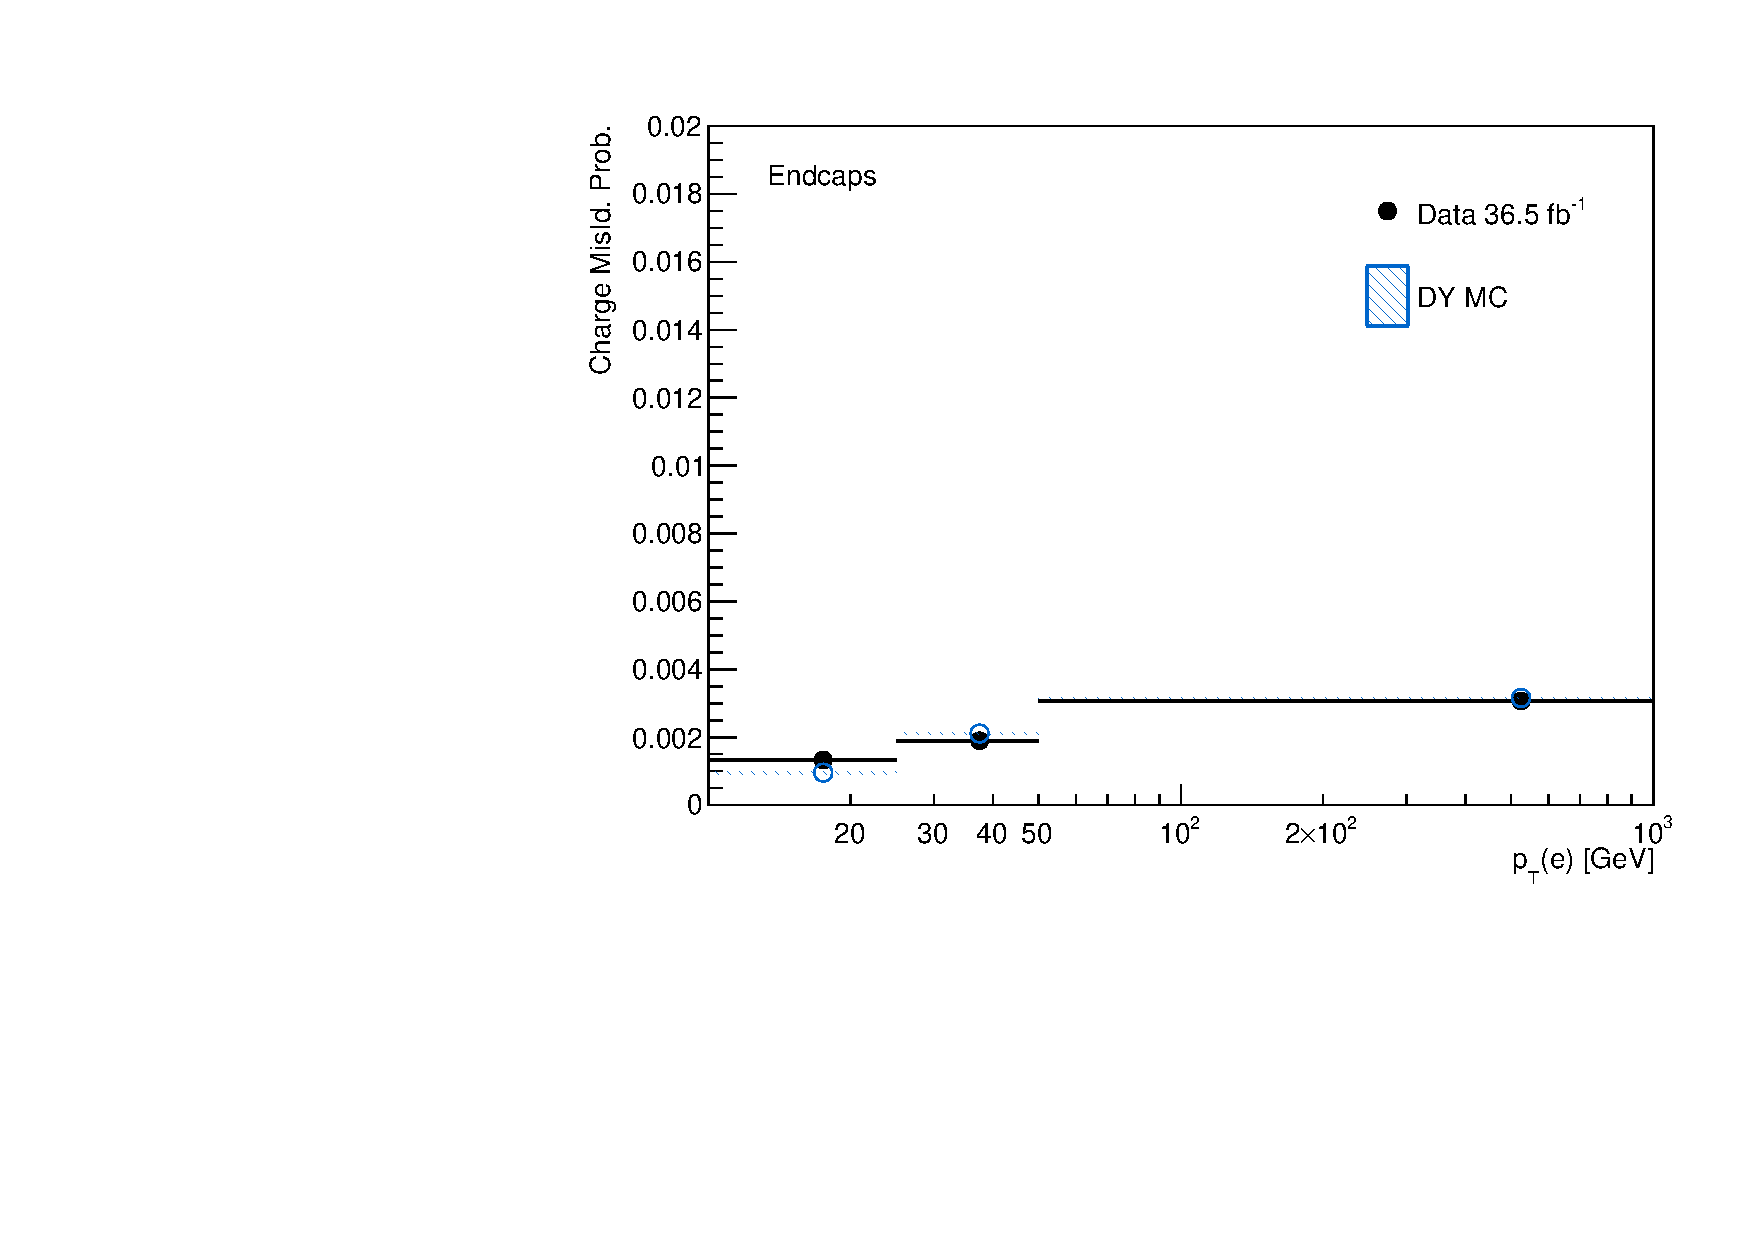
\includegraphics[width=0.49\textwidth]{chmid_prob_endcap.pdf}
\caption[Elecron mis-ID probabilities.]{Electron charge mis-ID probabilities as a function of \pt\ for |\etac|<2.5 (left) and |\etac|<2.5 (right) \cite{CMS_AN_2017-029}.}
\label{fig:chmisid_prob}
\end{figure}                            

The contribution from charge mis-ID electrons in signal selection of this analysis comes mainly from \ttbar\ and Drell-Yan events. The systematic uncertainty of the normalization of the charge mis-ID estimate is evaluated at about 30\%, arising from a slight disagreement of the mis-ID probability between data and simulation. Given that it only affects the $e\mu$ channel, its impact on the final sensitivity is very limited.

\section{Pre-selection yields}

The expected and observed event yields of the pre-selection are shown in Table \ref{tab:yields-sel}; Figure~\ref{fig:input_vars_presel} shows the distributions of some relevant kinematic variables, normalized to the cross section of the respective processes and to the integrated luminosity. The remaining variable distributions are shown in Appendix \ref{app:presel_plots}. 

%% \begin{table}[thb]
%% \centering
%% \begin{tabular}{lrrrr}\hline
%% \multicolumn{1}{c@{\qquad}}{} & \multicolumn{1}{c@{\qquad}}{$3\ell$} & \multicolumn{1}{c}{$\mumu$} & \multicolumn{1}{c@{\qquad}}{$\emu$} & \multicolumn{1}{c}{$\ee$} \\ \hline
%% $\ttW$                        & $  22.50 \pm 0.35$ & $ 68.03 \pm 0.61 $ & $ 97.00 \pm 0.71 $ & $ 29.63 \pm  0.39 $ \\
%% $\ttZ\!/\!\gamma^*$           & $  32.80 \pm 1.79$ & $ 25.89 \pm 1.12 $ & $ 64.82 \pm 2.42 $ & $ 28.74 \pm  1.70 $ \\
%% $\WZ$                         & $   8.22 \pm 0.86$ & $ 15.07 \pm 1.19 $ & $ 26.25 \pm 1.57 $ & $  9.31 \pm  0.93 $ \\
%% $\ZZ$                         & $   1.62 \pm 0.33$ & $  1.16 \pm 0.29 $ & $  2.86 \pm 0.45 $ & $  1.09 \pm  0.27 $ \\
%% $W^\pm W^\pm qq$              & --                 & $  3.96 \pm 0.52 $ & $  6.99 \pm 0.69 $ & $  2.19 \pm  0.37 $ \\
%% $W^\pm W^\pm \text{(DPS)}$    & --                 & $  2.48 \pm 0.42 $ & $  4.17 \pm 0.54 $ & $  0.81 \pm  0.24 $ \\
%% VVV                           & $   0.42 \pm 0.16$ & $  2.99 \pm 0.34 $ & $  4.85 \pm 0.43 $ & $  1.19 \pm  0.21 $ \\
%% $\mathrm{tttt}$               & $   1.84 \pm 0.44$ & $  2.32 \pm 0.45 $ & $  4.06 \pm 0.57 $ & $  0.89 \pm  0.31 $ \\
%% $\mathrm{tZq}$                & $   3.92 \pm 1.48$ & $  5.77 \pm 2.24 $ & $ 10.73 \pm 3.03 $ & $  7.56 \pm  1.72 $ \\
%% $\mathrm{tZW}$                & $   1.70 \pm 0.12$ & $  2.13 \pm 0.13 $ & $  3.91 \pm 0.18 $ & $  1.13 \pm  0.10 $ \\
%% $\gamma$ conversions          & $   7.43 \pm 1.94$ & --                 & $ 23.81 \pm 6.04 $ & $  9.87 \pm  4.17 $ \\ \hline
%% Non-prompt                    & $  25.61 \pm 1.26$ & $ 80.94 \pm 2.02 $ & $135.34 \pm 2.83 $ & $ 47.72 \pm  1.79 $ \\
%% Charge mis-ID                 & --                 & --                 & $ 58.50 \pm 0.31 $ & $ 44.52 \pm  0.31 $ \\ \hline
%% All backgrounds               & $ 106.05 \pm 3.45$ & $210.74 \pm 3.61 $ & $443.30 \pm 8.01 $ & $184.65 \pm  5.29 $ \\ \hline
%% $\tHq$ ($\Ct=-1.0$)           & $   7.48 \pm 0.14$ & $ 18.48 \pm 0.22 $ & $ 27.41 \pm 0.27 $ & $  8.47 \pm  0.15 $ \\
%% $\tHW$ ($\CV=-1.0$)           & $   7.38 \pm 0.16$ & $  7.72 \pm 0.17 $ & $ 11.23 \pm 0.20 $ & $  3.66 \pm  0.11 $ \\
%% $\ttH$                        & $  18.29 \pm 0.41$ & $ 24.18 \pm 0.48 $ & $ 35.21 \pm 0.58 $ & $ 11.07 \pm  0.32 $ \\ \hline
%% Data (35.9\fbinv)             & \multicolumn{1}{l}{127}&\multicolumn{1}{l}{280} & \multicolumn{1}{l}{525} & \multicolumn{1}{l}{208}\\\hline
%% \end{tabular}
%% \caption{Expected and observed yields for $35.9\fbinv$ after the pre-selection in all final states. Uncertainties are statistical only.}
%% \label{tab:yields-sel}
%% \end{table}

\begin{table}[thb]
\centering
\begin{tabular}{lrrr}\hline
\multicolumn{1}{c@{\qquad}}{} & \multicolumn{1}{c@{\qquad}}{$3\ell$} & \multicolumn{1}{c}{$\mumu$} & \multicolumn{1}{c@{\qquad}}{$\emu$} \\ \hline
$\ttW$                        & $  22.50 \pm 0.35$ & $ 68.03 \pm 0.61 $ & $ 97.00 \pm 0.71 $  \\
$\ttZ\!/\!\gamma^*$           & $  32.80 \pm 1.79$ & $ 25.89 \pm 1.12 $ & $ 64.82 \pm 2.42 $  \\
$\WZ$                         & $   8.22 \pm 0.86$ & $ 15.07 \pm 1.19 $ & $ 26.25 \pm 1.57 $  \\
$\ZZ$                         & $   1.62 \pm 0.33$ & $  1.16 \pm 0.29 $ & $  2.86 \pm 0.45 $  \\
$W^\pm W^\pm qq$              & --                 & $  3.96 \pm 0.52 $ & $  6.99 \pm 0.69 $  \\
$W^\pm W^\pm \text{(DPS)}$    & --                 & $  2.48 \pm 0.42 $ & $  4.17 \pm 0.54 $  \\
VVV                           & $   0.42 \pm 0.16$ & $  2.99 \pm 0.34 $ & $  4.85 \pm 0.43 $  \\
$\mathrm{tttt}$               & $   1.84 \pm 0.44$ & $  2.32 \pm 0.45 $ & $  4.06 \pm 0.57 $  \\
$\mathrm{tZq}$                & $   3.92 \pm 1.48$ & $  5.77 \pm 2.24 $ & $ 10.73 \pm 3.03 $  \\
$\mathrm{tZW}$                & $   1.70 \pm 0.12$ & $  2.13 \pm 0.13 $ & $  3.91 \pm 0.18 $  \\
$\gamma$ conversions          & $   7.43 \pm 1.94$ & --                 & $ 23.81 \pm 6.04 $  \\ \hline
Non-prompt                    & $  25.61 \pm 1.26$ & $ 80.94 \pm 2.02 $ & $135.34 \pm 2.83 $  \\
Charge mis-ID                 & --                 & --                 & $ 58.50 \pm 0.31 $  \\ \hline
All backgrounds               & $ 106.05 \pm 3.45$ & $210.74 \pm 3.61 $ & $443.30 \pm 8.01 $  \\ \hline
$\tHq$ ($\Ct=-1.0$)           & $   7.48 \pm 0.14$ & $ 18.48 \pm 0.22 $ & $ 27.41 \pm 0.27 $  \\
$\tHW$ ($\CV=-1.0$)           & $   7.38 \pm 0.16$ & $  7.72 \pm 0.17 $ & $ 11.23 \pm 0.20 $  \\
$\ttH$                        & $  18.29 \pm 0.41$ & $ 24.18 \pm 0.48 $ & $ 35.21 \pm 0.58 $  \\ \hline
Signal + Backgrounds          & $ 139.20 \pm 3.49$ & $261.12 \pm 3.65 $ & $517.15 \pm 8.03 $  \\ \hline
Data (35.9 fb$^{-1}$)         & \multicolumn{1}{c}{127}&\multicolumn{1}{c}{280} & \multicolumn{1}{c}{525} \\\hline
\end{tabular}
\caption[Expected and observed yields for 35.9 \fbinv after the pre-selection.]{Expected and observed yields for 35.9 \fbinv after the pre-selection in all final states. Uncertainties are statistical only.}
\label{tab:yields-sel}
\end{table}

\begin{figure}[!htb]
\centering
        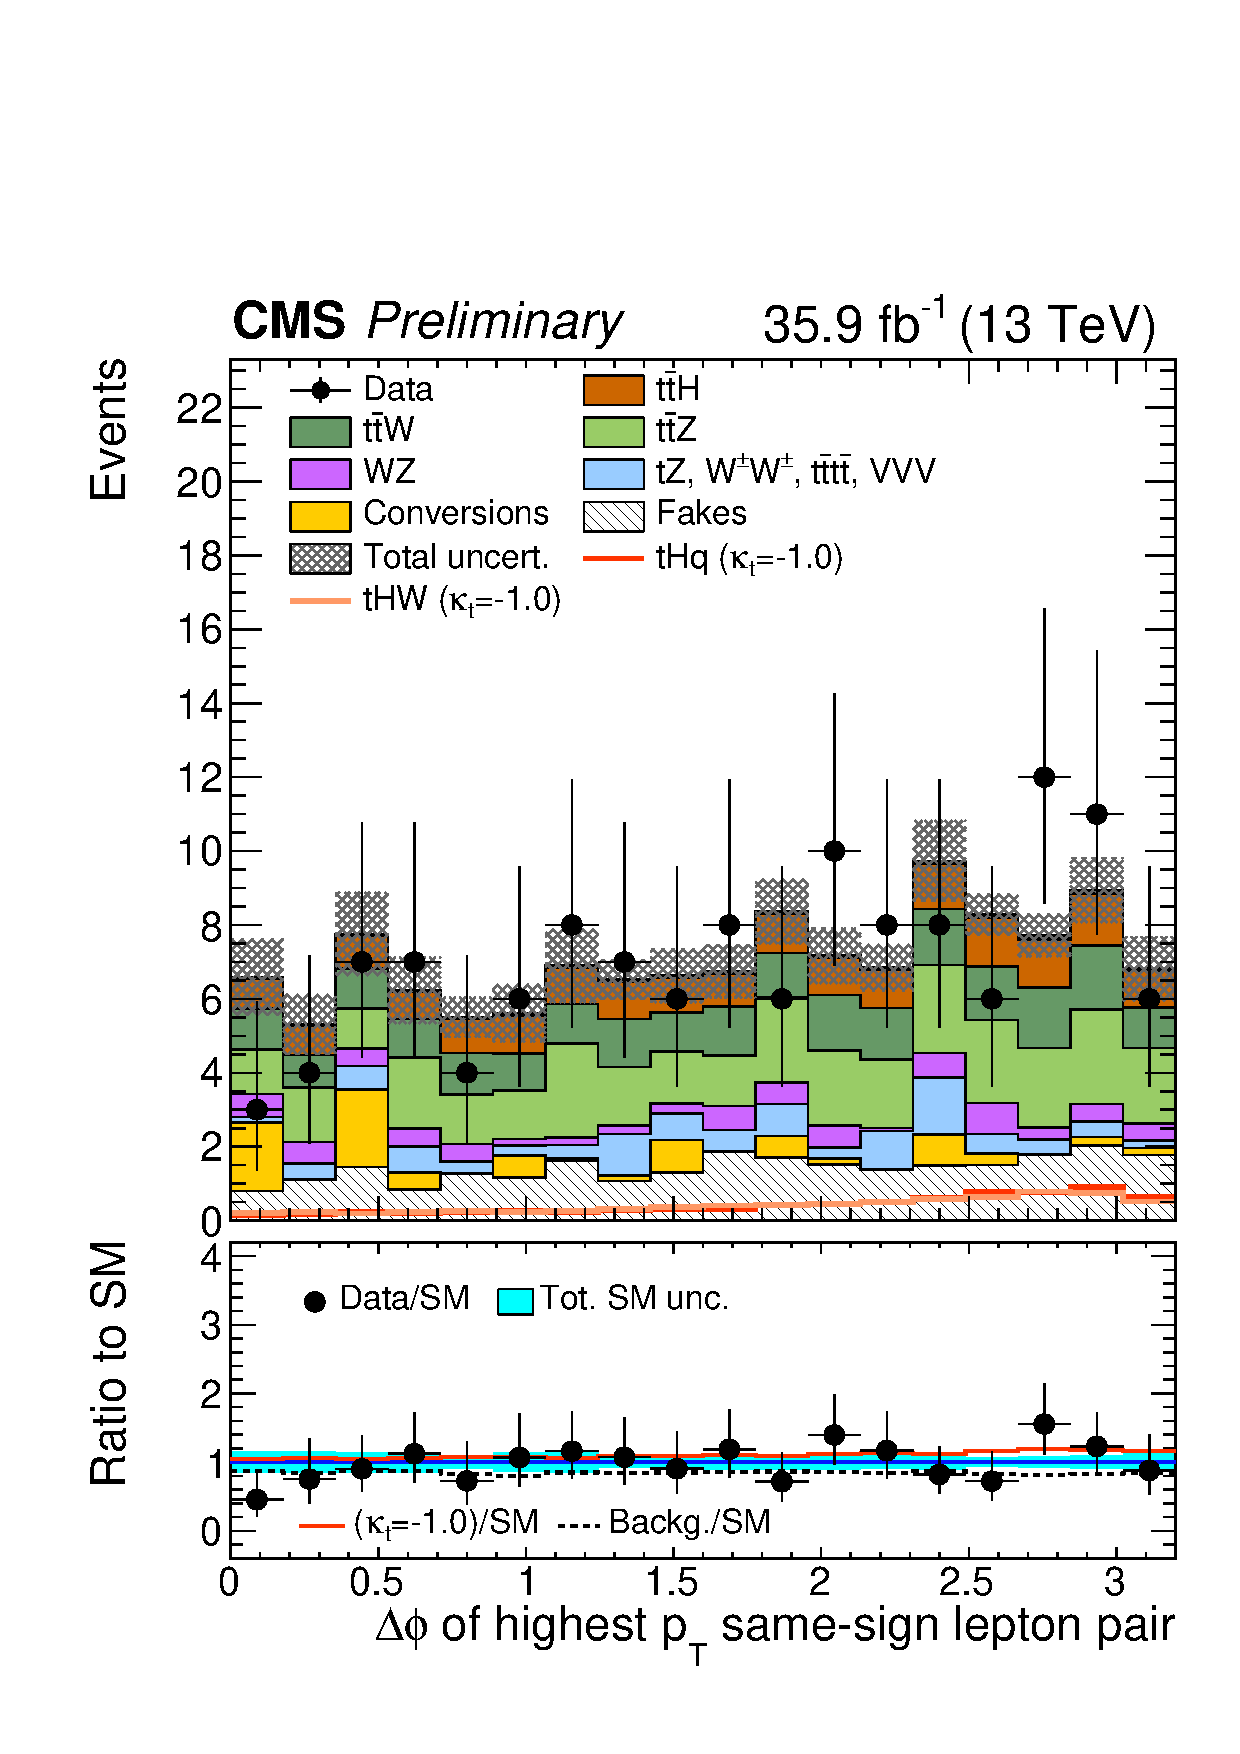
\includegraphics[width=0.31\linewidth]{polished/dPhiHighestPtSSPair_3l.pdf}
        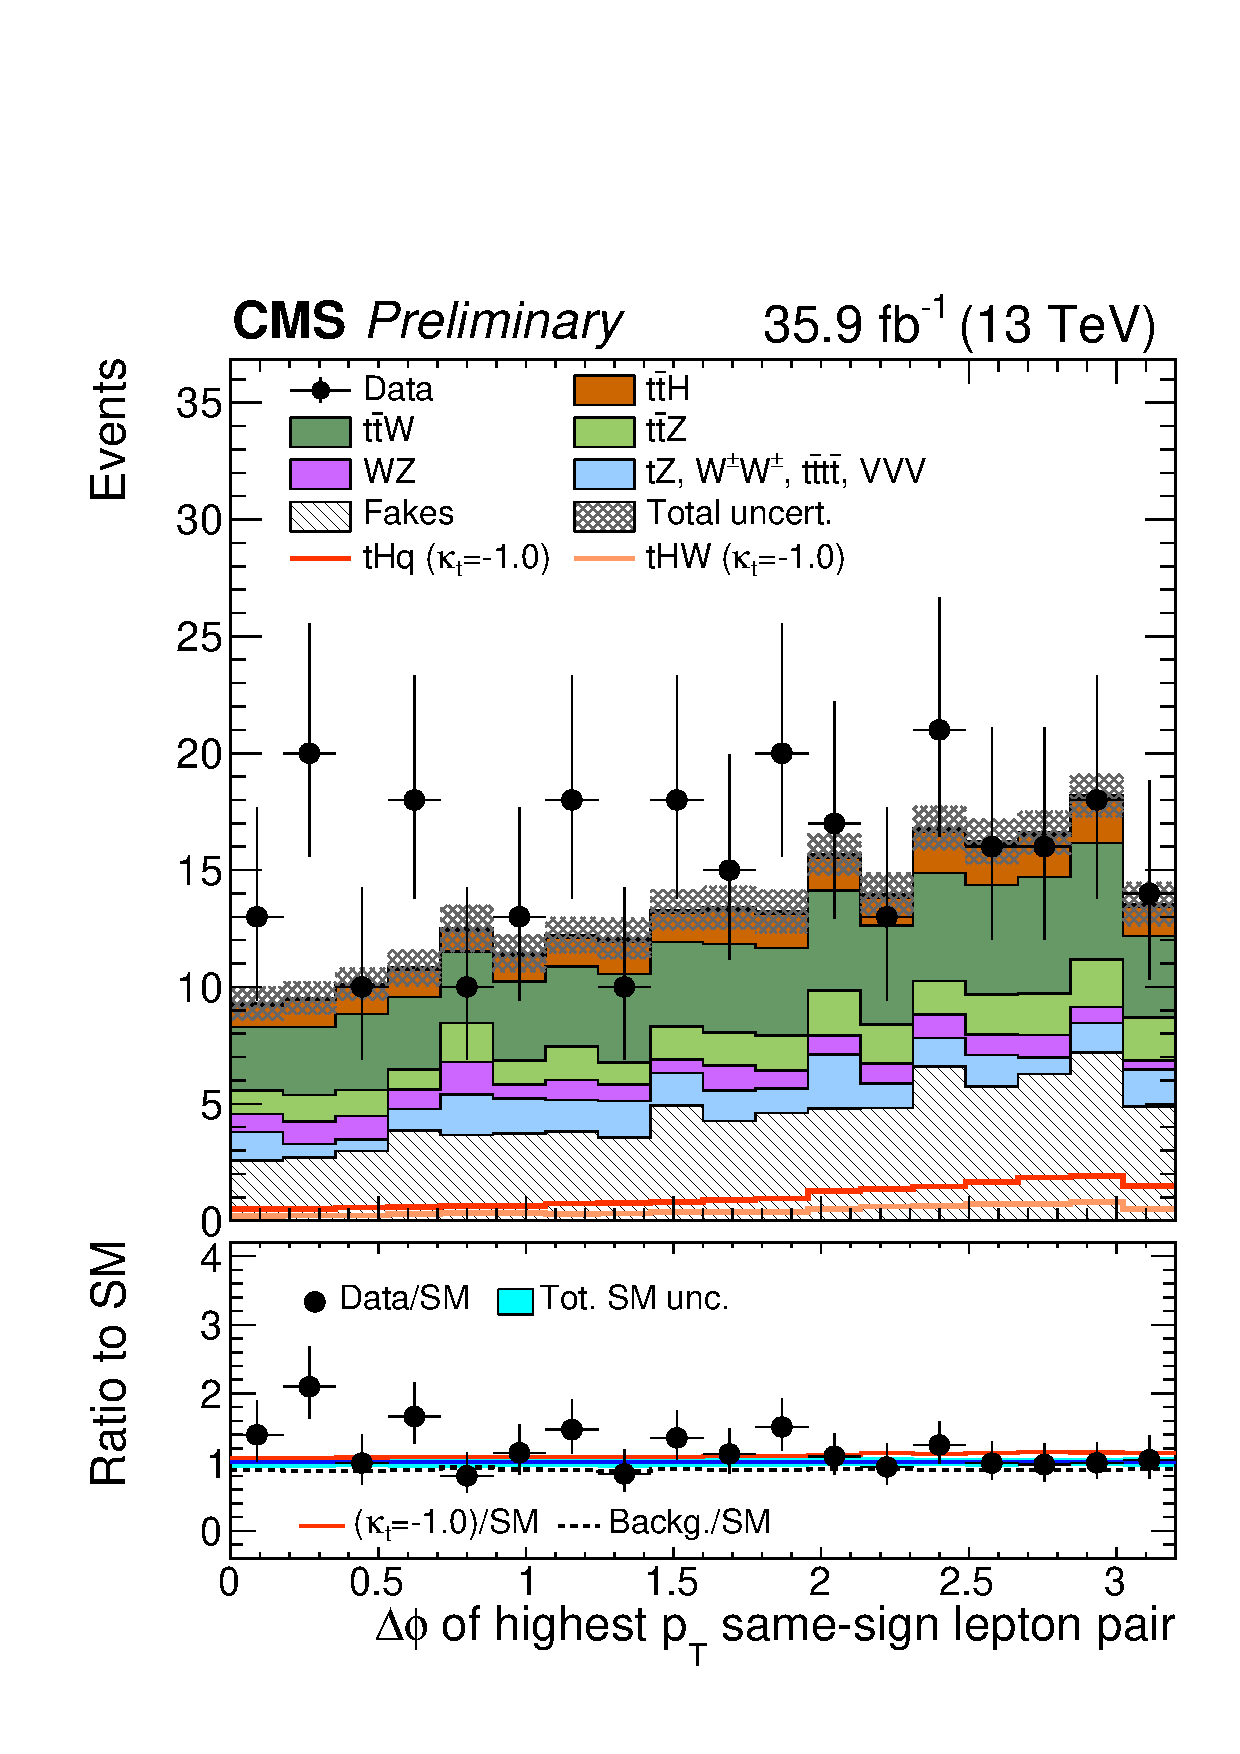
\includegraphics[width=0.31\linewidth]{polished/dPhiHighestPtSSPair_mm.pdf}              
        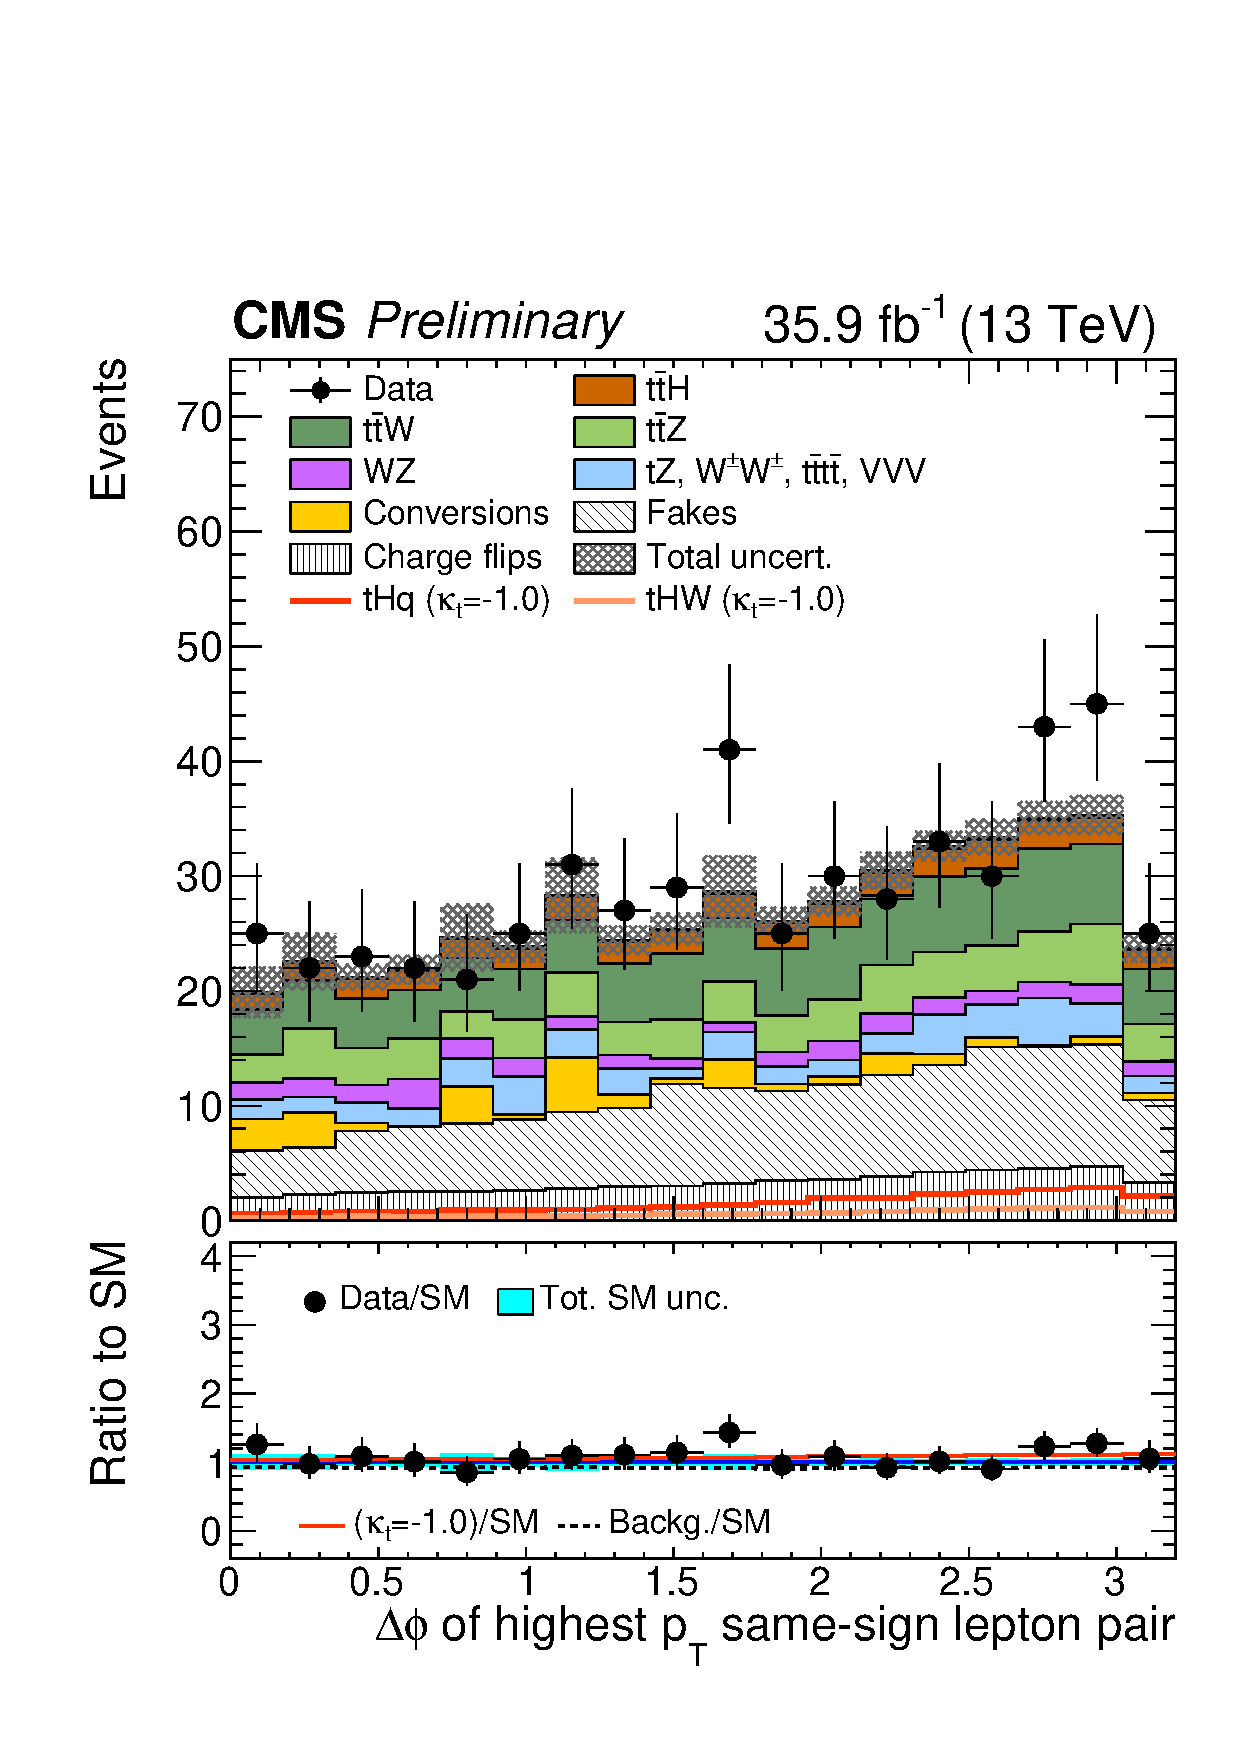
\includegraphics[width=0.31\linewidth]{polished/dPhiHighestPtSSPair_em.pdf}\\
        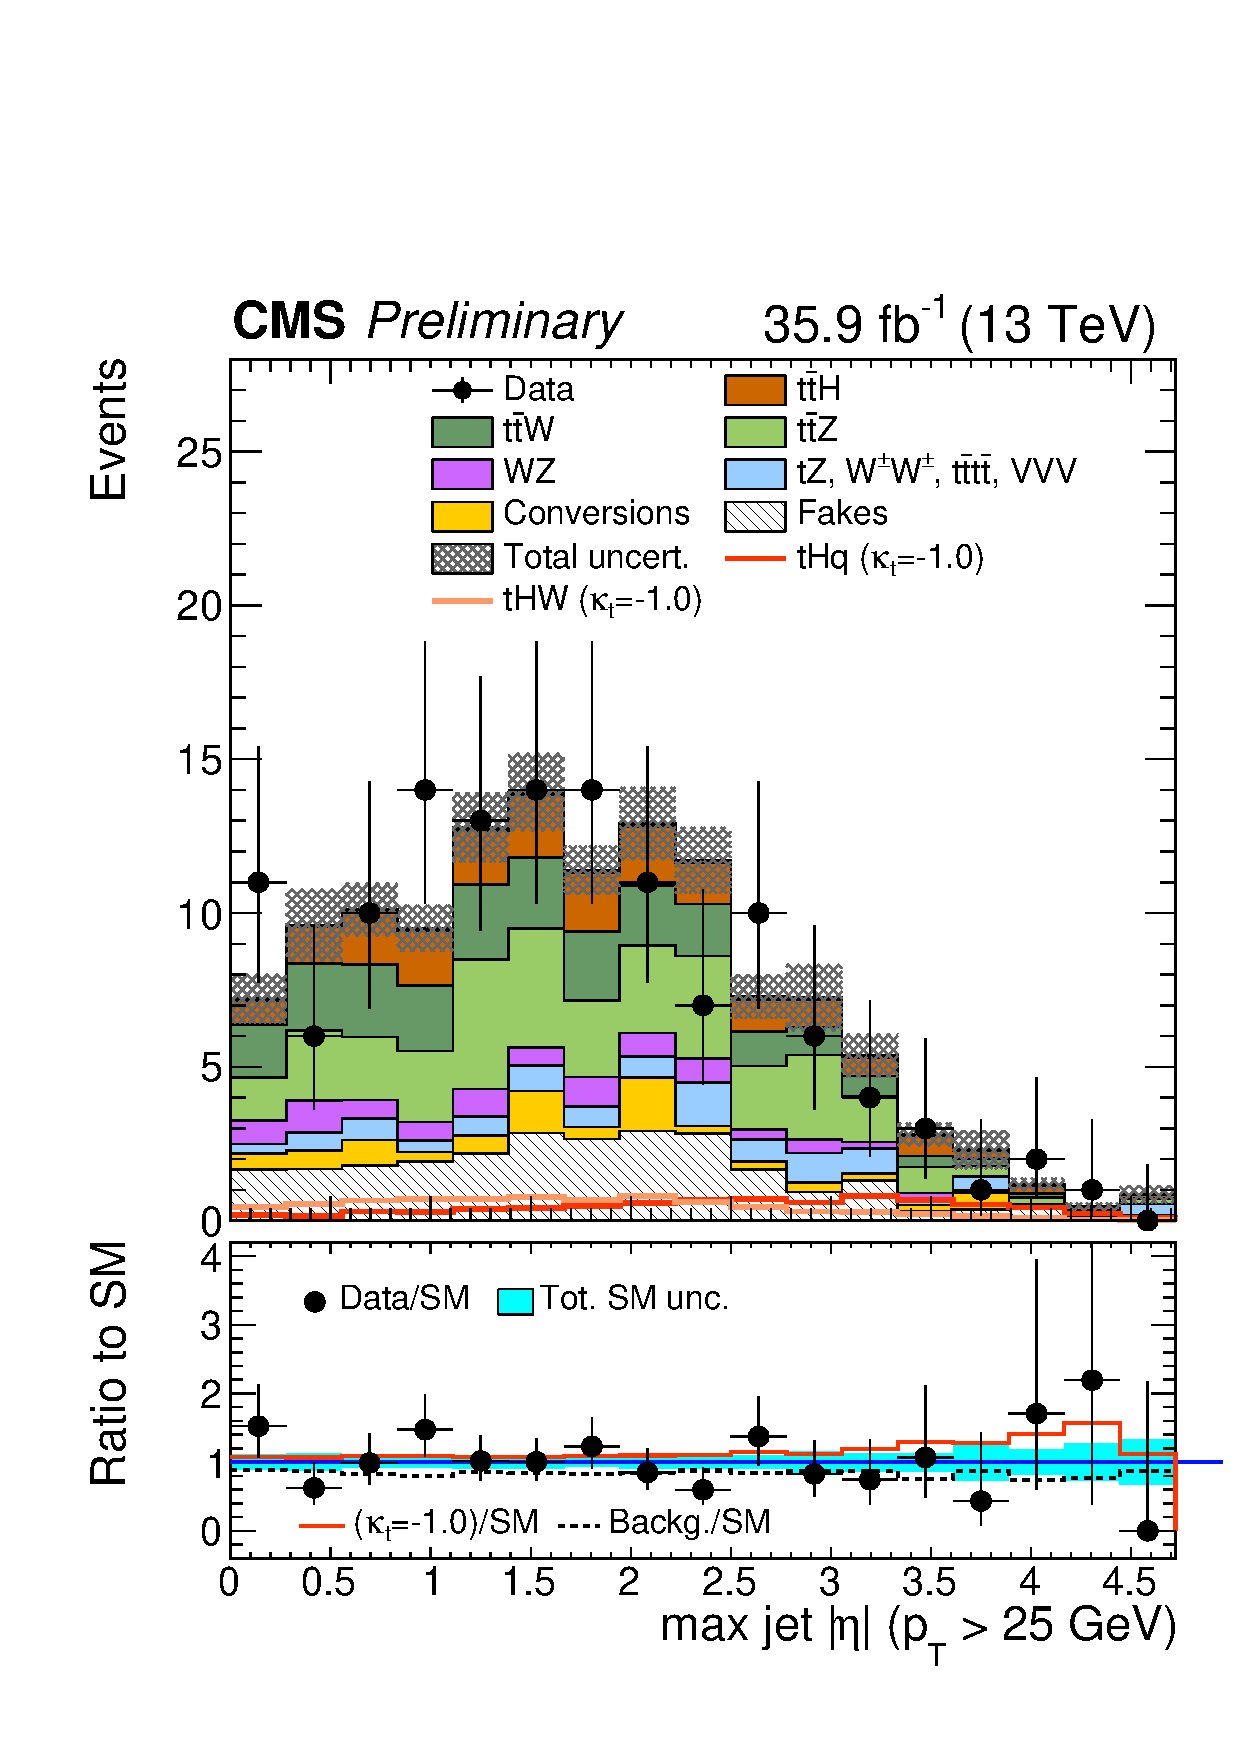
\includegraphics[width=0.31\linewidth]{polished/maxEtaJet25_40_3l.pdf}
        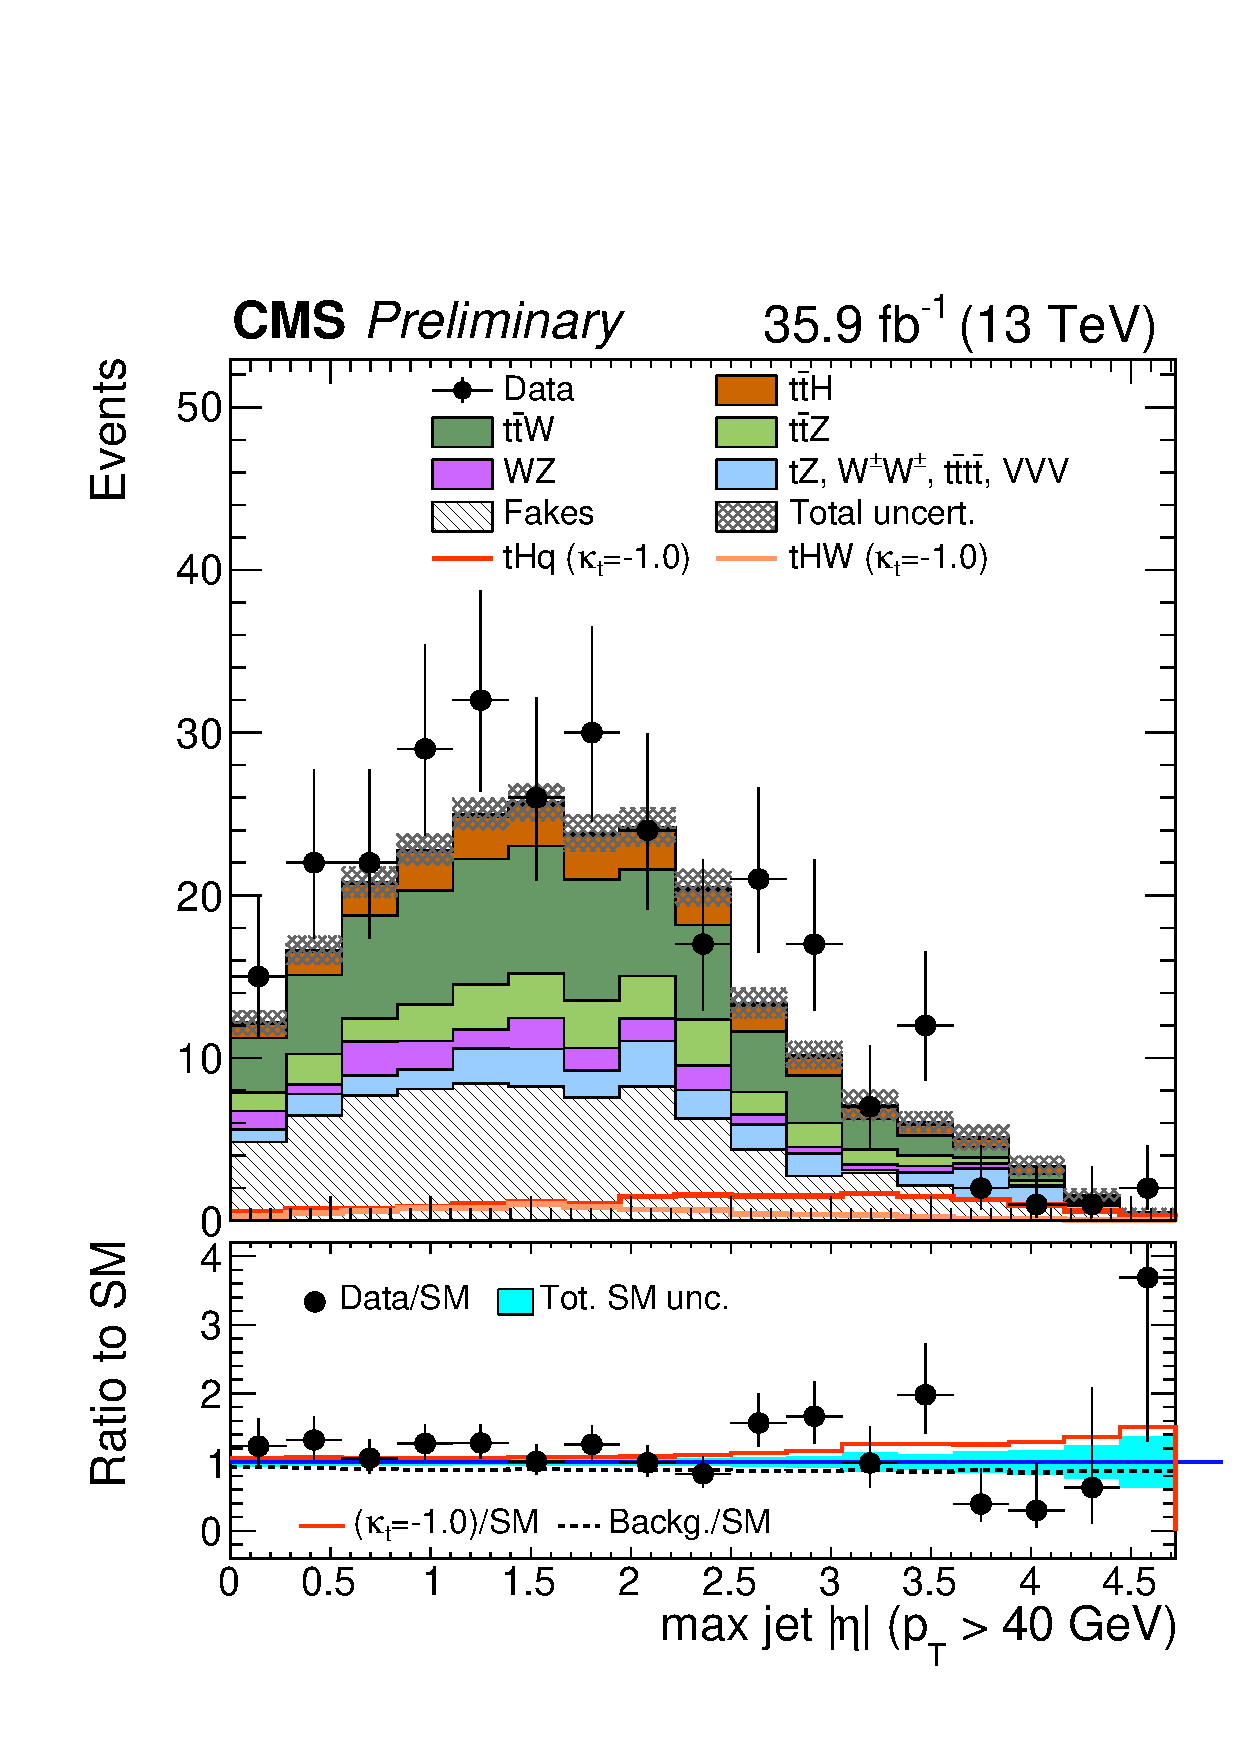
\includegraphics[width=0.31\linewidth]{polished/maxEtaJet25_40_mm.pdf}
        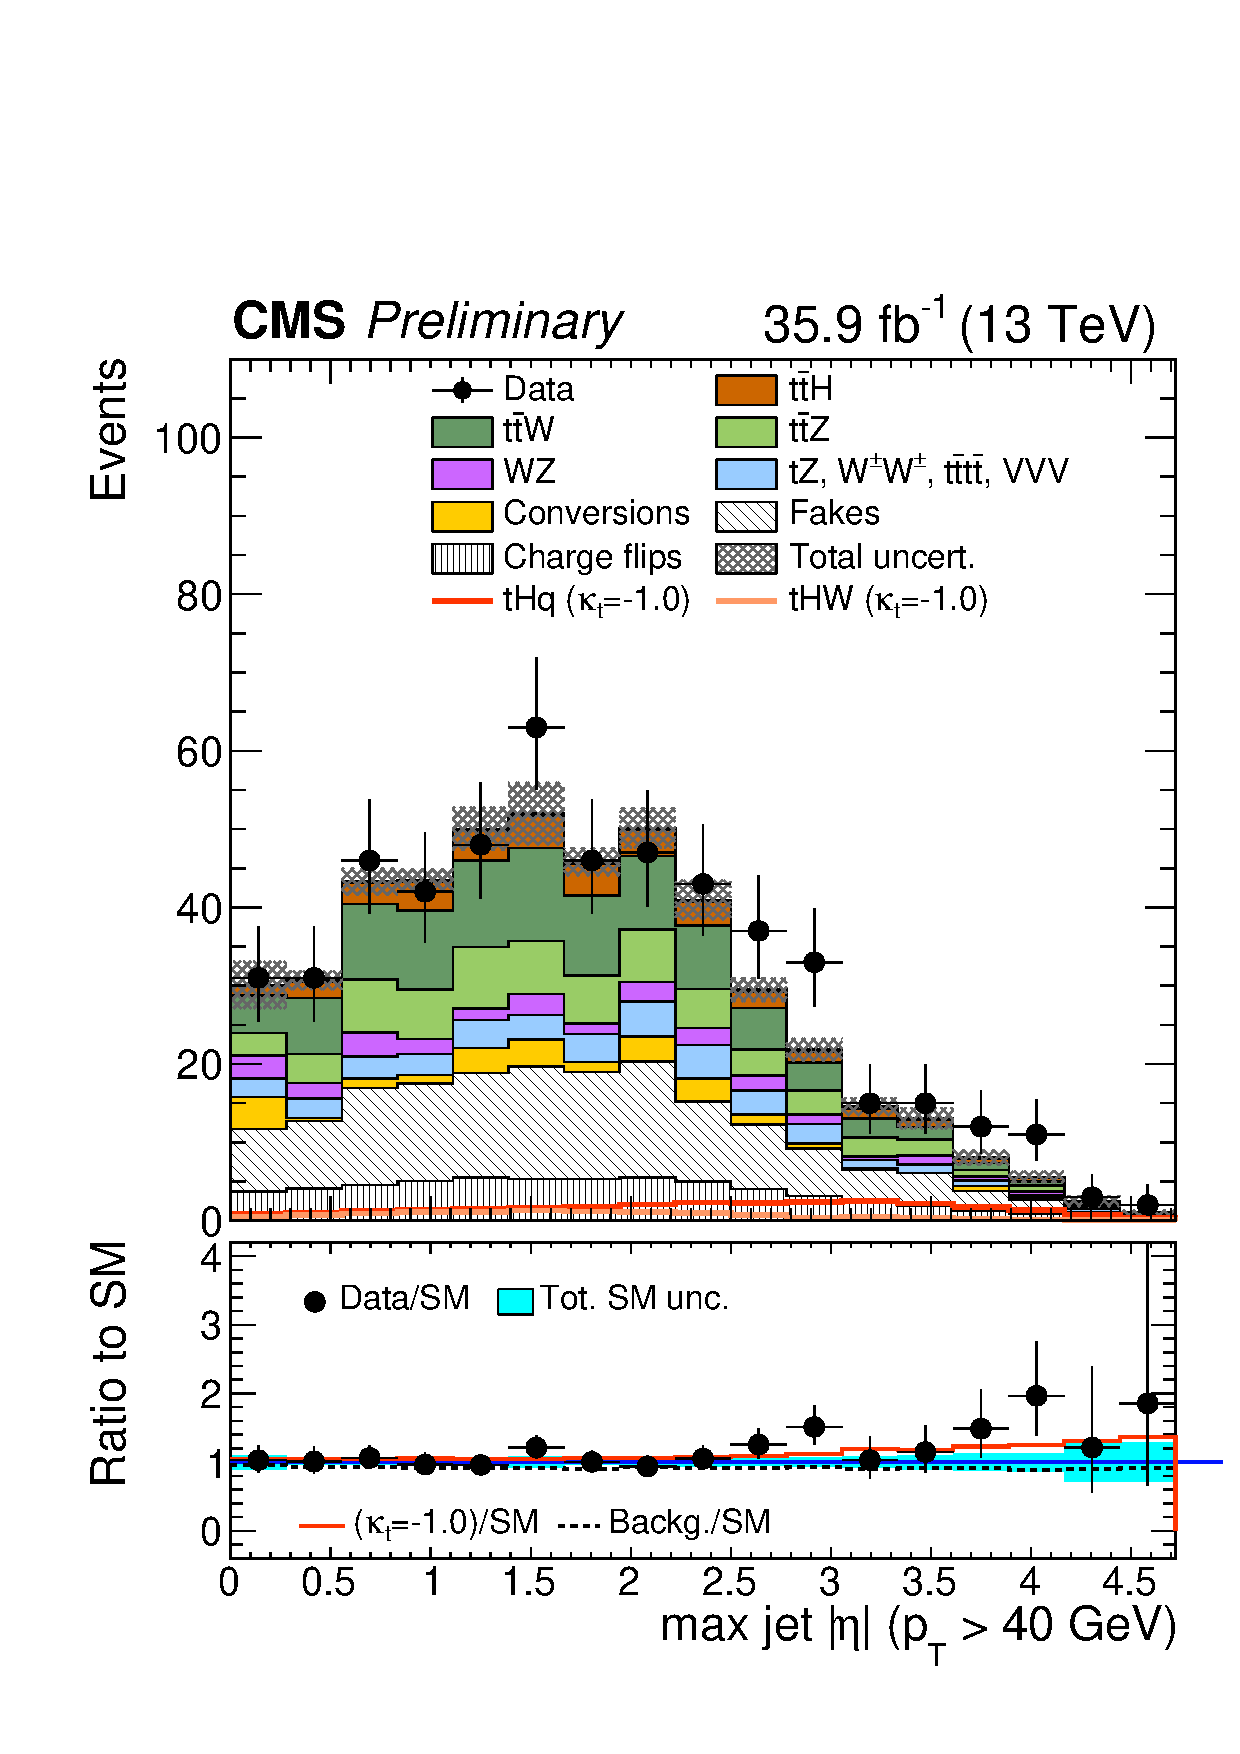
\includegraphics[width=0.31\linewidth]{polished/maxEtaJet25_40_em.pdf}\\  
        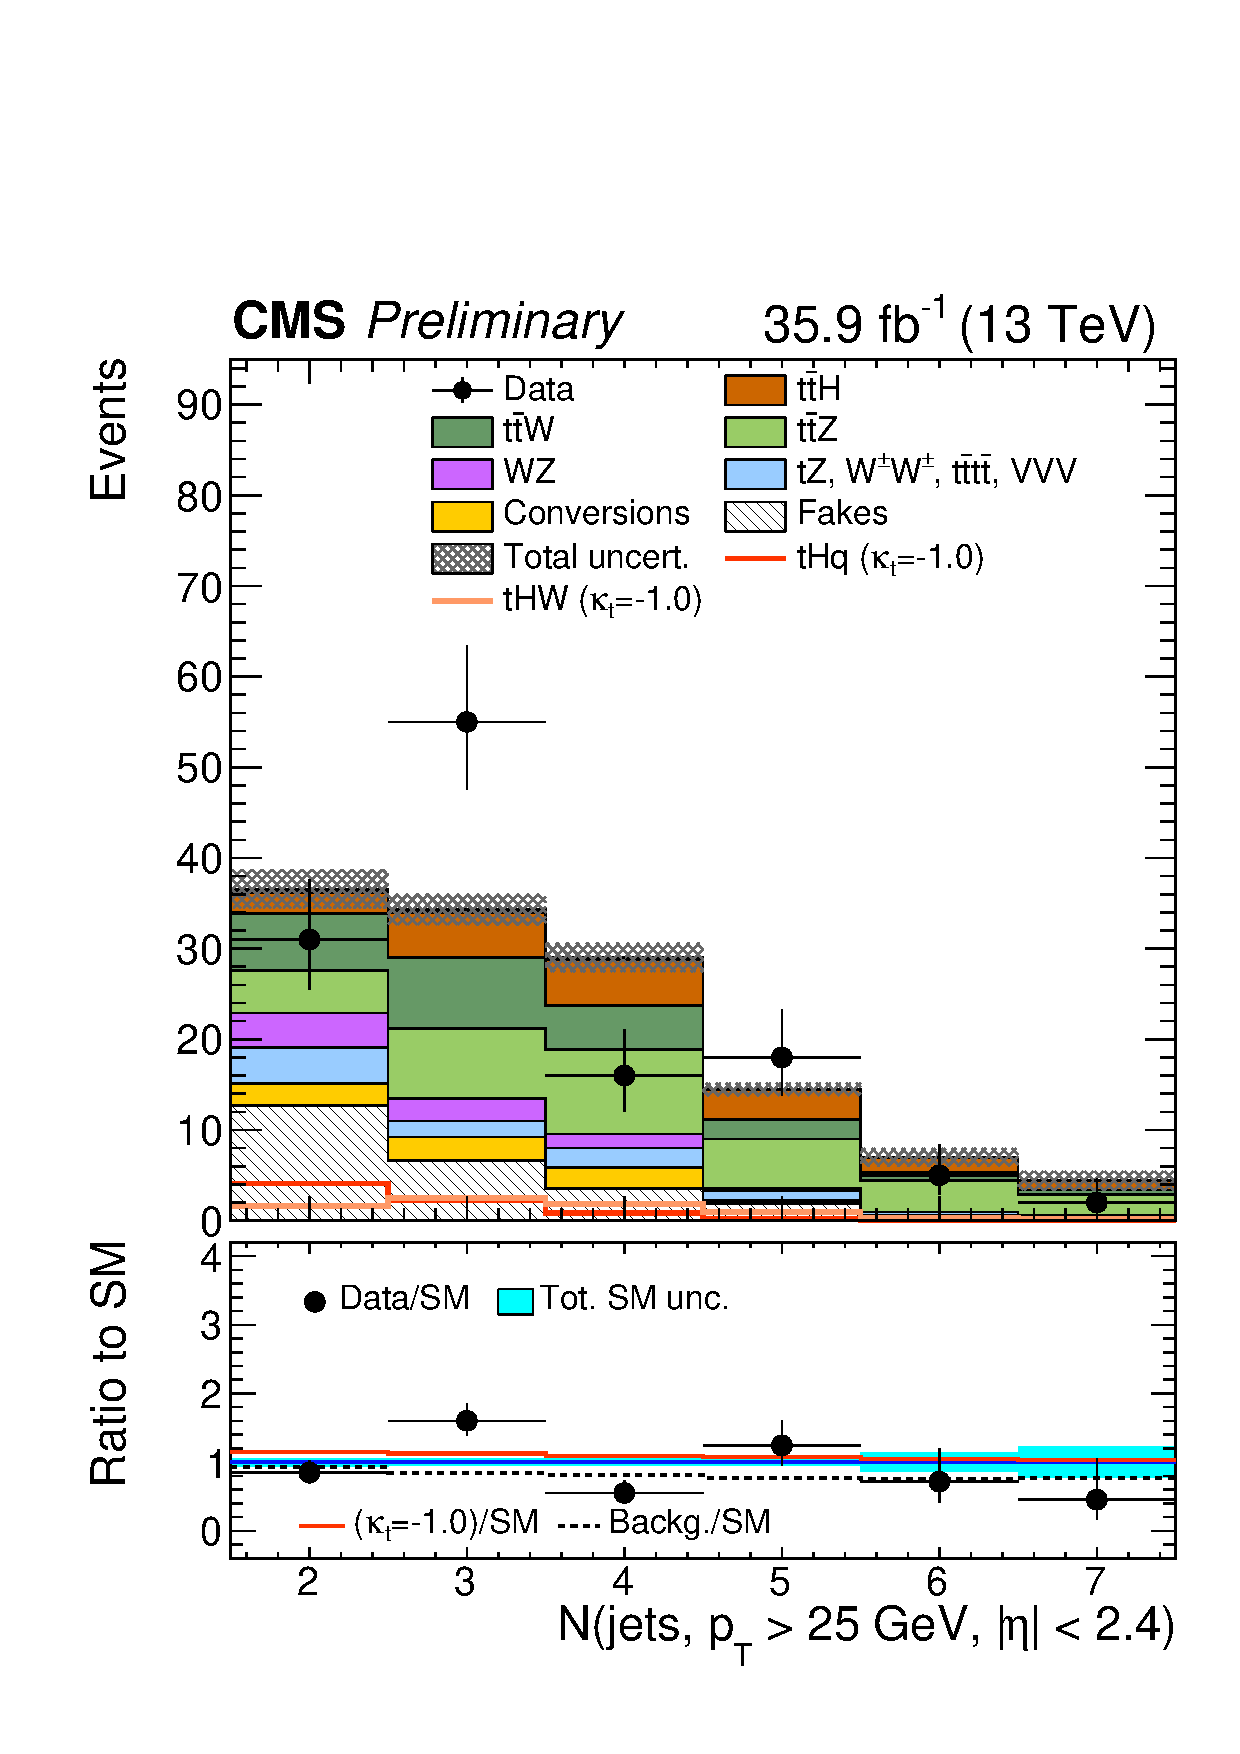
\includegraphics[width=0.31\linewidth]{polished/nJet25_3l.pdf}                    
        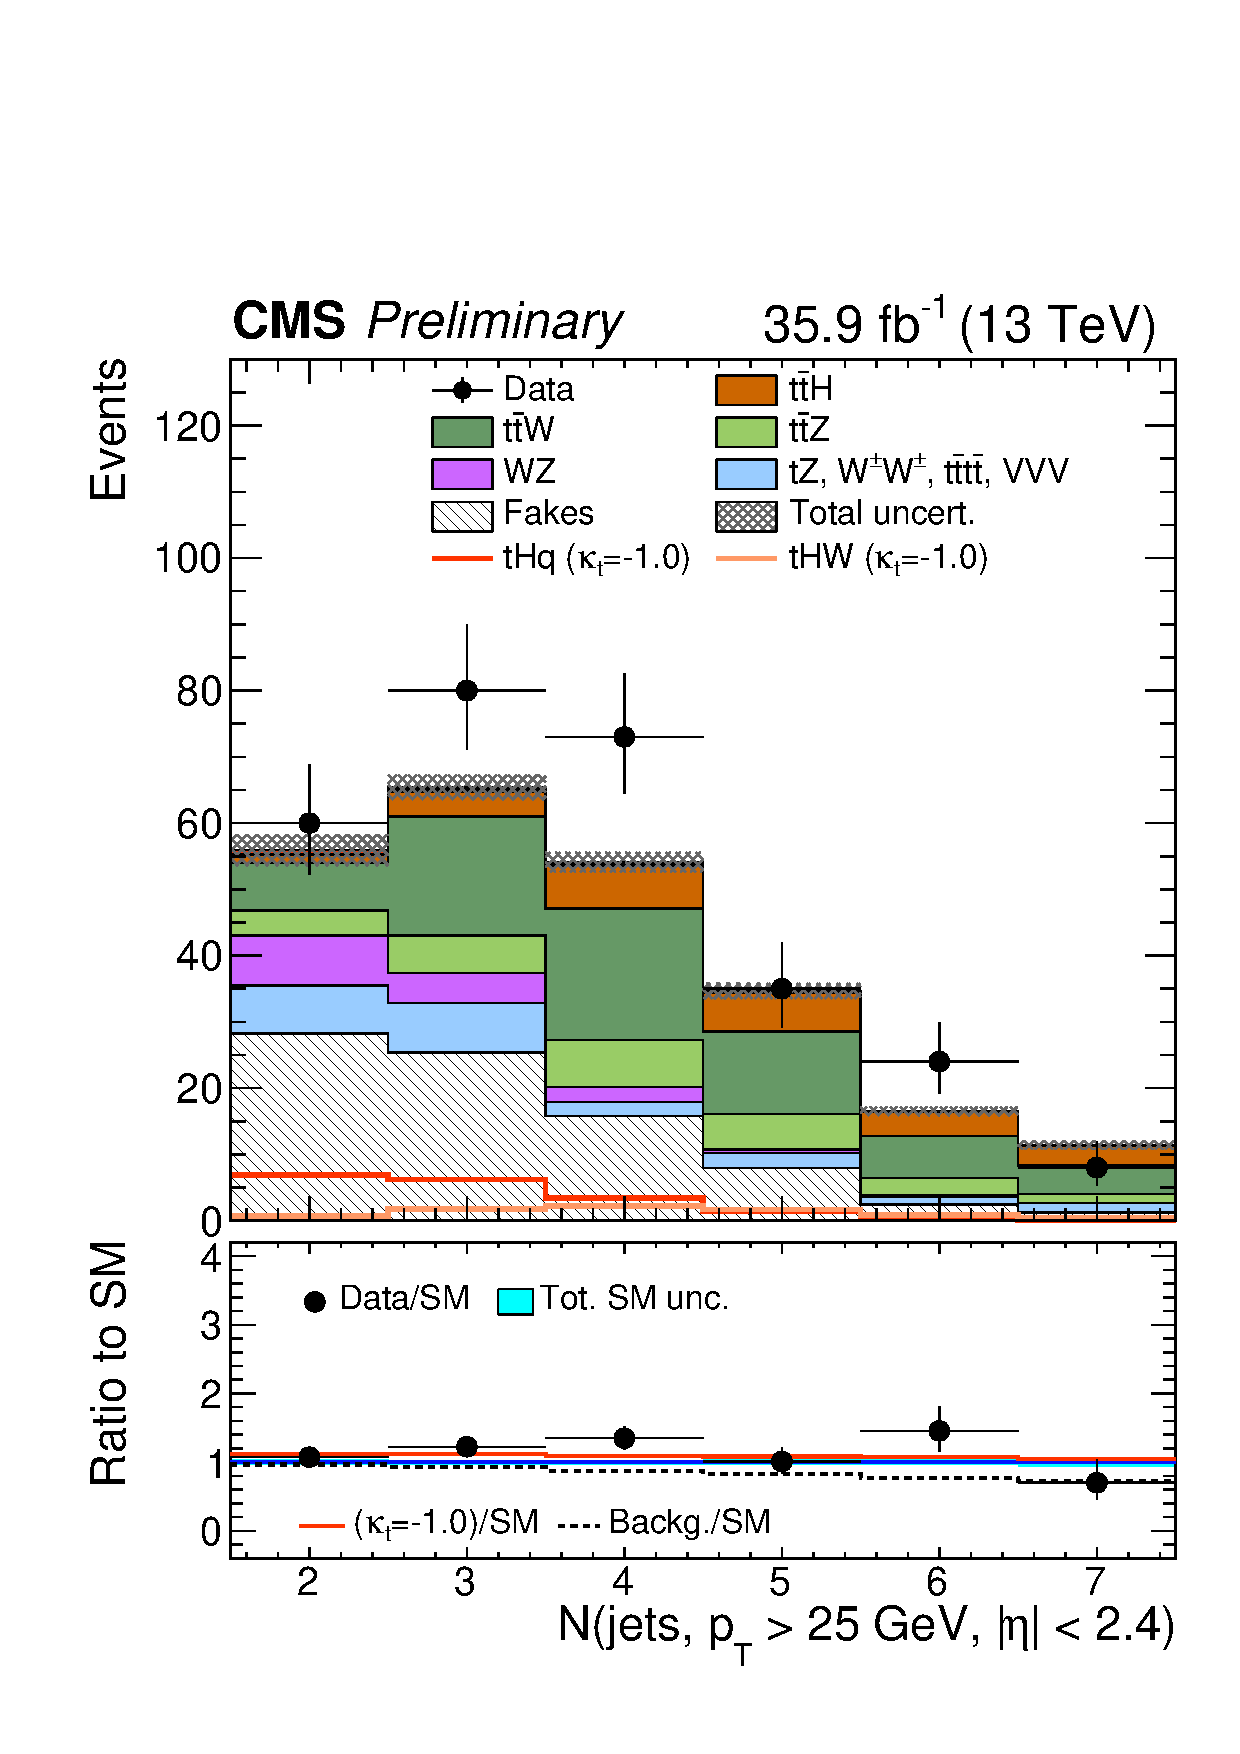
\includegraphics[width=0.31\linewidth]{polished/nJet25_mm.pdf} 
        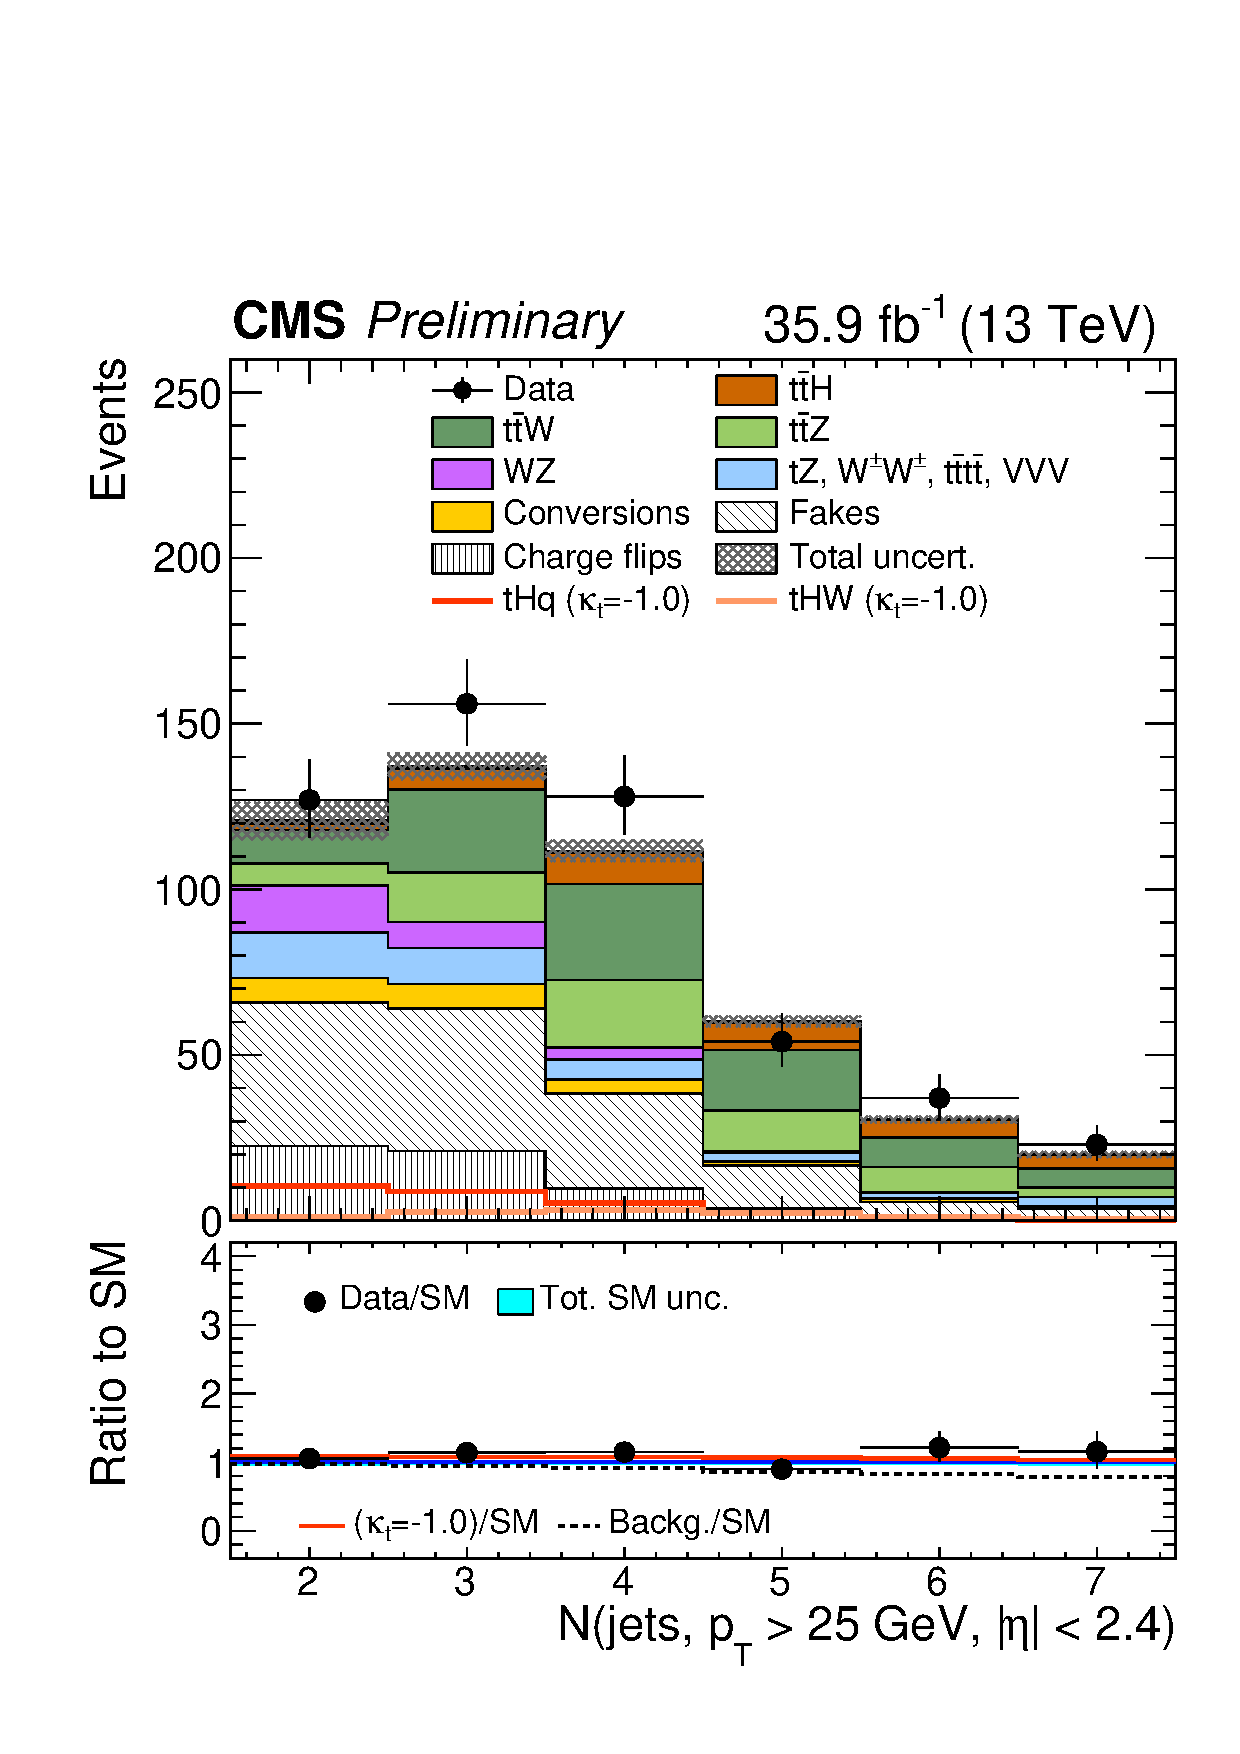
\includegraphics[width=0.31\linewidth]{polished/nJet25_em.pdf} 
\caption[Discriminating variables for the event pre-selection.]{Distributions of discriminating variables for the event pre-selection for the three lepton channel (left column), same-sign \mumu\ channel (middle column), the same-sign \emu\ channel (right column), normalized to 35.9\ \fbinv, before fitting the signal discriminant to the observed data. Uncertainties are statistical and unconstrained (pre-fit) normalization systematics. The shape of the two \tH\ signals for $\Ct=-1.0$ is shown, normalized to their respective cross sections for $\Ct=-1.0, \CV=1.0$.}
\label{fig:input_vars_presel}
\end{figure}

For the \tH\ and \ttH processes, the largest contribution comes from Higgs decays to WW (about 75\%), followed by \tautau (about 20\%) and ZZ (about 5\%). Other Higgs production modes contribute negligible event yields (< 5\% of the \tH +\ttH yield) as shown in Table ~\ref{tab:yield_hbr}. Table~\ref{tab:presel_eff} shows the acceptance$\times$efficiency for the pre-selection criteria in Table~\ref{tab:cuts}.   

\begin{table}[!hbt]
\centering
\begin{tabular}{lrrrr}\hline
\multicolumn{1}{c@{\qquad}}{} & \multicolumn{2}{c@{\qquad}}{$3\ell$} & \multicolumn{2}{c}{$\mumu$} \\ \hline
$\tHq (\mathrm{Inclusive})$   & $\mathbf{6.57}$     & 100.0\%  & $\mathbf{17.38}$ & 100.0\% \\
$\tHq (H\to WW)$              & $4.84$   & 73.9\%   & $13.33 $ &  76.9\%  \\
$\tHq (H\to \tau\tau)$        & $1.04$   & 15.9\%   & $ 3.62 $ &  20.6\%  \\
$\tHq (H\to ZZ)$              & $0.48$   &  7.2\%   & $ 0.37 $ &   2.2\%  \\
$\tHq (H\to \mu\mu)$          & $0.21$   &  3.0\%   & $ 0.04 $ &   0.2\%  \\
$\tHq (H\to \gamma\gamma)$    & $<0.01$  &  0.1\%   & $ 0.02 $ &   0.1\%  \\
$\tHq (H\to bb)$              & $<0.01$  & $<0.1$\% & $ 0.01 $ & $<0.1$\% \\ \hline
$\tHW (\mathrm{Inclusive})$   & $\mathbf{7.32}$ & 100.0\% & $\mathbf{7.62}$ & 100.0\% \\
$\tHW (H\to WW)$              & $5.50 $ &  76.9\%  & $ 5.60$ & 74.1\% \\
$\tHW (H\to \tau\tau)$        & $1.40 $ &  20.6\%  & $ 1.81$ & 23.1\% \\
$\tHW (H\to ZZ)$              & $0.31 $ &   2.2\%  & $ 0.21$ &  2.7\% \\
$\tHW (H\to \mu\mu)$          & $0.12 $ &   0.2\%  & $ 0.01$ &  0.1\% \\
$\tHW (H\to \gamma\gamma)$    & $<0.01$ & $<0.1$\% & $<0.01$ &$<0.1$\% \\
$\tHW (H\to bb)$              & $<0.01$ & $<0.1$\% & $<0.01$ &$<0.1$\% \\ \hline
\end{tabular}
\caption[Signal yields split by decay channels of the Higgs boson.]{Signal yields split by decay channels of the Higgs boson. Forward jet \pt cut at 25 GeV.}
\label{tab:yield_hbr}
\end{table}

\begin{table}[!thb]
\centering
\begin{tabular}{lrrr}\hline
\multicolumn{1}{c@{\qquad}}{} & \multicolumn{1}{c@{\qquad}}{$3\ell$} & \multicolumn{1}{c}{$\mumu$} & \multicolumn{1}{c@{\qquad}}{$\emu$} \\ \hline
$\ttW$                        & $ 0.25 $ & $ 0.75 $ & $ 1.07$  \\
$\ttZ\!/\!\gamma^*$           & $ 0.36 $ & $ 0.29 $ & $ 0.71$  \\
$\tHq$ ($\Ct=-1.0$)           & $ 0.03 $ & $ 0.06 $ & $ 0.10$  \\
$\tHW$ ($\CV=-1.0$)           & $ 0.14 $ & $ 0.15 $ & $ 0.21$  \\
$\ttH$                        & $ 0.24 $ & $ 0.32 $ & $ 0.46$  \\ \hline
\end{tabular}
\caption[Acceptance$\times$efficiency for pre-selection cut.]{Acceptance$\times$efficiency (\%) for signal and main background events pre-selection.}
\label{tab:presel_eff}
\end{table}

A significant fraction of selected data events (about 50\% in the dilepton channels, and about 80\% in the trilepton channel) also passes the selection used in the dedicated search for \ttH in multilepton channels \cite{CMS_AN_2017-029}. This is particularly important when considering a possible combination of the measurements from both studies. More details about the overlap between these two analyses are presented in Appendix \ref{app:overlap}.   

%______________________ Signal discrimination ______________________
\section{Signal discrimination }
\label{secc:signal_disc}

The production cross sections for the signal processes \tHq, \tHW, and \ttH is only about 600 fb (the enhancement provided by inverted couplings, \Ct = -1 almost double them), resulting in a small signal to background ratio even for a tight selection. A multivariate method is hence employed to train discriminators to separate \tH\ signal events from the dominant background events.

\subsection{MVA classifiers evaluation}

Several MVA classifier algorithms were evaluated in order to determine the most appropriate method for this analysis\footnote{The choice of the tested algorithms was based on the recommendations provided by the official TMVA user guide, the experience from previous analyses and considering the expertise of the members of the \tHq and \ttH analyses groups. Only the BDT classifier is described in this thesis and a detailed description of all available methods can be found in Reference \cite{tmva}.}. The comparison is based on the performance of the classifiers, encoded in the plot of the background rejection as a function of the signal efficiency (ROC curve). The top row of Figure~\ref{roc} shows the ROC curves for evaluated methods; two separated trainings were performed in the $3l$ channel: against \ttbar\ (right) and \ttV\ (left) processes.

\begin{figure} [!h]
  \centering
   \includegraphics[width=0.49\textwidth]{roc_ttv_3l_multimva.pdf}
   \includegraphics[width=0.49\textwidth]{roc_tt_3l_multimva.pdf} \\
   \includegraphics[width=0.49\textwidth]{roc_ttv_2lss.pdf}
   \includegraphics[width=0.49\textwidth]{roc_tt_2lss.pdf} 

\caption[MVA classifiers performance.]{ Top: Background rejection vs signal efficiency (ROC curves) for various MVA classifiers in the $3l$ channel for training against \ttV\ (left) and \ttbar\ (right). Bottom: background rejection vs signal efficiency (ROC curve) in the $2lss$ channel for a single discriminator: BDTG, against \ttV\ (left) and \ttbar\ (right).}
\label{roc}
\end{figure} 

In both cases, the gradient boosted decision tree \ti{BDTG} (BDTA\_GRAD in the plot) classifier offers the best results, followed by the adaptive BDT classifier (\ti{BDTA}); the several Fisher classifiers tested, which differ in their parameters and/or boosting method, offer similar performance among them, while the k-Nearest Neighbour (kNN) classifier performance is below the rest of the classifiers. The corresponding ROC curves and in the $2lss$ channel for trainings against \ttV (left) and \ttbar (right) processes are shown in the bottom row of Figure~\ref{roc}; the BDTG performance is similar to that in the $3l$ channel.

\subsection{Discriminating variables}

The classifier chosen to separate the \tHq signal from the main backgrounds is the BDTG classifier, trained on simulated signal and background events. The samples used in the training are the \tHq sample in Table \ref{tab:sigsamples}, the samples marked with an * in Table \ref{tab:bgsamples} and the samples in the third section in Table \ref{tab:bgsamples}.

As explained in Section \ref{subsec:dt}, a set of discriminating variables are given as input to the BDTG which combines the individual discrimination power of each input variable to produce a quantity with the maximum discrimination power. Table~\ref{tab:bdtinputs} lists the input variables used in the BDTG trainings for this analysis. The same set of input variables was used to produce the plots for MVA classifiers evaluation. 

\begin{table}[h!]
\centering
\begin{tabular}{lp{10cm}}\hline
Variable name        & Description\\ \hline
nJet25               & Number of jets with $\pt>25$ GeV, $|\eta|<2.4$\\
nJetEta1             & Number of jets with $|\eta|>1.0$, non-CSV-loose\\\hline
MaxEtaJet25          & Max. $|\eta|$ of any (non-CSV-loose) jet with $\pt>25$ GeV\\
detaFwdJetClosestLep & $\Delta \eta$ forward light jet and closest lepton\\
detaFwdJetBJet       & $\Delta \eta$ forward light jet and hardest CSV loose jet\\
detaFwdJet2BJet      & $\Delta \eta$ forward light jet and second hardest CSV loose jet \\\hline
Lep3Pt/Lep2Pt        & \pt\ of the $3^{rd}$ lepton ($2^{nd}$ for 2lss)\\
totCharge            & Sum of lepton charges \\
minDRll              & Min $\Delta R$ any two leptons\\
dphiHighestPtSSPair  & $\Delta \phi$ of highest \pt\ same-sign lepton pair\\\hline
\end{tabular}
\caption[BDTG input variables.]{BDTG input variables. First section lists variables related to jet multiplicity, second section lists variables related to forward jet activity and variables related to lepton kinematics are listed in third section.}
\label{tab:bdtinputs}
\end{table}

\begin{figure} [!h]
 \centering
 \includegraphics[width=\textwidth]{input_var_diag}
\caption[Diagrams for \tHq, \ttbar, and \ttW  processes.]{BDT input variables are defined based on the features of the signal and background processes. Diagrams for signal and the two dominant backgrounds: \tHq (left), \ttbar (middle) and \ttW (right) processes. The second \bjet in \tHq process, indicated in the diagram as an opaque jet, originates from the spectator $\bar{b}$ quark remaining from the gluon splitting into a $b\bar{b}$ pair.} 
\label{fig:input_vars_diag}
\end{figure}    

BDTG input variables reflect those features that differentiate the signal process from the background processes.

The first two input variables in Table~\ref{tab:bdtinputs} are related to the jet multiplicity in the events. As shown in the diagrams of the Figure~\ref{fig:input_vars_diag}, signal events are expected to have one forward jet, one \bjet, and two (zero) light jets in the $2lss(3l)$ channel. Note that in the $2lss$ channel light jets originate from a W boson which could be off-shell; if one of these jets is too soft ($\pt<25$ GeV) it does not get reconstructed and the event is not identified as a signal event. In the case of \ttbar events, one \bjet and two light jets (zero for $3l$ channel) are expected, one fewer that for signal events. For \ttW events, the number of jets is the same as for signal events but usually there are more final state radiation jets than in signal. Thus, nJet25 accounts for the number of jets in the event while nJetEta1 accounts for the number of forward jets.  
            
The second section of variables in Table~\ref{tab:bdtinputs} is related to the forward jet activity and the location of the leptons and other jets with respect to the forward jet; leptons and \bjets are expected to be central in both signal and background events. MaxEtaJet25 evaluates how forward are jets in the event. detaFwdJetClosestLep evaluates how separated in \etac the forward jet is from the leptons and \bjets in the event; in background events leptons and jets are central and then closer to each other than in signal events where this separation is large. The same reasoning applies for detaFwdJetBjet.

detaFwdJet2Bjet evaluates the separation in \etac between the light forward jet and the second \bjet. As described in Chapter \ref{ch:theory}, in the four flavor scheme, b quarks are not allowed inside the proton, therefore, the incoming $b$ quark involved in \tHq process is originated from a gluon splitting into a $b\bar{b}$ pair, hence, the second \bjet in \tHq process comes from the remaining $\bar{b}$ quark acting as a spectator and appearing in the final state as a forward \bjet. This second \bjet tends to be very forward and then it is not always reconstructed. For signal events with two forward jets, one forward and the other backward, detaFwdJet2Bjet would be larger than for background events with two \bjets for which \bjets are central and then less separated from the light forward jet. 

The third section of variables in Table~\ref{tab:bdtinputs} is related to the lepton kinematics encoding the distinctive behavior of leptons in signal events and background events. In \tHq and \ttbar events, same-sign leptons are back to back; for three lepton events, the two opposite sign leptons are closer together. In \ttW events, leptons tends to be distributed throughout the space; thus minDRll and dphiHighestPtSSPair account for these features.       

Lep2Pt and Lep3Pt represent the \pt of the second and third lepton in $2lss$ and $(3l)$ events respectively. In \ttbar the fake lepton is expected to have lower \pt than the corresponding lepton in signal events; in \ttW events, all leptons are expected to be high \pt leptons, therefore their correspondent leptons in signal events are expected to have lower \pt.

Finally, totCharge is the sum of the lepton charges in the final state; for \tHq events, it is expected to be asymmetrically distributed with an excess of positive charge because the proton have more $u$ quarks that $d$ quarks, therefore, more W$^+$ bosons are expected and then more positive leptons in the final state. The total charge in \ttbar events is expected to be symmetrically distributed since the final state is neutral while for \tHW events the distribution is expected to be asymmetric due to the presence of the W boson. 

Plots in Figure~\ref{fig:input_vars_3l} shows the BDTG input variables distributions for the signal and background samples in the $3l$ channels; these plots exhibit the features described above. 

\begin{figure} [!h]
 \centering
 \includegraphics[width=0.32\textwidth]{maxEtaJet25.pdf}
 \includegraphics[width=0.32\textwidth]{dEtaFwdJetClosestLep.pdf}
 \includegraphics[width=0.32\textwidth]{dEtaFwdJetBJet.pdf}\\
 \includegraphics[width=0.32\textwidth]{dEtaFwdJet2BJet.pdf}
 \includegraphics[width=0.32\textwidth]{Lep3Pt.pdf}
 \includegraphics[width=0.32\textwidth]{totCharge.pdf}\\
 \includegraphics[width=0.32\textwidth]{minDRll.pdf}
 \includegraphics[width=0.32\textwidth]{dPhiHighestPtSSPair.pdf}
 \includegraphics[width=0.32\textwidth]{nJet25.pdf}\\      
 \includegraphics[width=0.32\textwidth]{nJetEta1.pdf}
\caption[BDTG classifier Input variables distributions.]{Distributions of the BDTG classifier input variables for signal discrimination, normalized to equal area, in the $3l$ channel.} 
\label{fig:input_vars_3l}
\end{figure}    

All the input variables have some discrimination power, however, that power is bigger for some of them. For instance, the third lepton \pt plot (top left in Figure~\ref{fig:input_vars_3l}) shows some discrimination power against WZ and VVV backgrounds; although this variable discriminates only against these two backgrounds, it is useful for the overall background discrimination.

The same or equivalent input variables are found to perform well for both $3l$ and $2lss$ channels. Figure~\ref{fig:input_vars_2lss} shows the corresponding input variables distribution plots for the $2lss$ channel.

\subsubsection*{Discrimination power from BDTG classifier}

%% \begin{figure} [!h]
%%   \centering
%%   \includegraphics[width=\textwidth]{mva_input1_tt.pdf}
%%   \includegraphics[width=\textwidth]{mva_input2_tt.pdf}
%% \caption[BDT input variables. Discrimination against \ttbar in $3l$ channel.]{BDT input variables as seen by BDTG classifier for the $3l$ channel, \tHq signal (blue) discriminated against \ttbar\ background (red).} 
%% \label{mva_input_tt}
%% \end{figure}

The discrimination power of the input variables can also be evaluated from the BDTG training, exclusively for the training samples, \ie, dominant backgrounds (\ttbar and \ttV); the training samples are submitted to the selection cuts on Table ~\ref{tab:cuts}.

\begin{figure} [!ht]
  \centering
  \includegraphics[width=\textwidth]{mva_input1.pdf}
  \caption[BDT input variables. Discrimination against \ttbar and \ttV\ in $3l$ channel.]{BDT input variables as seen by BDTG classifier for the $3l$ channel, \tHq (blue) discriminated against background (red), \ttbar (top) and \ttV (bottom).}
\label{fig:mva_input_comp}
\end{figure}

Figure~\ref{fig:mva_input_comp} shows the comparison between input variables for the two trainings in the $3l$ channel; it reveals that some variables show opposite behavior for the two background sources, which results in potentially screening the discrimination power if they were to be used in a single discriminant, \ie, if the training would join \ttbar and \ttV. For some other variables the distributions are similar in both background cases. In contrast to the distributions in Figure~\ref{fig:input_vars_3l} only the dominant backgrounds are included; however, the discrimination power agrees among plots.

Figures~\ref{mva_input_2lss_tt}, ~\ref{mva_input_2lss_ttv}, ~\ref{mva_input_tt}, and ~\ref{mva_input_ttv} show the input variables distributions for the $2lss$ and $3l$ channels as seen by the BDTG classifier. 

\subsubsection*{Input variables correlations}

\begin{figure} [!ht]
  \centering
      \includegraphics[width=0.32\textwidth]{sig_corr_tt_2lss.pdf}
      \includegraphics[width=0.32\textwidth]{bkg_corr_tt_2lss.pdf}
      \includegraphics[width=0.32\textwidth]{bkg_corr_ttv_2lss.pdf}\\
      \includegraphics[width=0.32\textwidth]{corr_signal.pdf}
      \includegraphics[width=0.32\textwidth]{corr_tt.pdf}
      \includegraphics[width=0.32\textwidth]{corr_ttv.pdf}
\caption[Correlation matrices for the BDT input variables.]{ Signal (left), \ttbar\ background (middle), and \ttV\ background (right.) correlation matrices for the input variables in the BDTG classifier for the $2lss$ (top) and  $3l$ (bottom) channels.}
\label{mva_corr}
\end{figure}

From Table~\ref{tab:bdtinputs}, it is clear that the input variables are correlated to some extent. These correlations play an important role for some MVA methods like the Fisher discriminant method in which the first step consist of performing a linear transformation to an phase space where the correlations between variables are removed. In the case of BDT, correlations do not affect the performance. Figure~\ref{mva_corr} shows the linear correlation coefficients for signal and background for the two training cases (the signal values are identical by construction). As expected, strong correlations appear for variables related to the forward jet activity.

\subsection{BDTG classifiers response}

After the training stage, the BDTG classifier is tested to ensure its ability to discriminate between simulated signal and background events. The BDTG classifier output distributions for signal and backgrounds in the $3l$ channel are shown in Figure~\ref{fig:bdtg_output_default}. As expected, a good discrimination power is obtained using default discriminator parameter values; some overtraining, represented in the differences between the test (histogram) and the training (dots), is also visible.

\begin{figure} [!h]
  \centering
   \includegraphics[width=0.49\textwidth]{bdta_grad_output_3l_ttv}
   \includegraphics[width=0.49\textwidth]{bdta_grad_output_3l_tt}
\caption[BDTG classifier response. Default parameters.]{BDTG classifier output for trainings against \ttV (left) and \ttbar(right). Default BDTG  parameters have been used.}
\label{fig:bdtg_output_default}
\end{figure}

In order to explore further optimization in the BDTG performance, several changes from the default BDTG parameters were tested; Table \ref{tab:bdtsettings} lists the set of parameters found to be most discriminant with minimal overtraining as shown in Figure~\ref{fig:output_2lss}.  

\begin{table} [!h]
\centering
\begin{tabular}{lll}\hline
  \verb|TMVA.Types.kBDT                  | \\\hline
  \verb|Option            Default   Used |\\
  \verb|NTrees            200       800  |\\
  \verb|BoostType         AdaBoost  Grad | \\
  \verb|Shrinkage         1         0.1  | \\ 
  \verb|nCuts             20        50   | \\
  \verb|MaxDepth          3              | \\ \hline
\end{tabular}
\caption[Configuration used in the final BDTG training.]{Configuration used in the final BDTG training. Parameters not listed were not tested.}\label{tab:bdtsettings}
\end{table}

\begin{figure} [!h]
  \centering
   \includegraphics[width=0.49\textwidth]{bdt_output_ttv_2lss.pdf}
   \includegraphics[width=0.49\textwidth]{bdt_output_tt_2lss.pdf}\\
   \includegraphics[width=0.49\textwidth]{bdt_response_ttv_3l.pdf}
   \includegraphics[width=0.49\textwidth]{bdt_response_tt_3l.pdf}
\caption[BDTG classifier output.]{BDTG classifiers output for training against \ttV\ (left) and \ttbar\ (right) for $2lss$ channel\ (top) and $3l$ channel\ (bottom) .}
\label{fig:output_2lss}
\end{figure}

%% \begin{table}[h!]
%% %\centering
%% \footnotesize
%% \begin{tabular}{llrlr}\hline
%%       &\multicolumn{2}{c}{$2lss$ channel}         & \multicolumn{2}{c}{$3l$ channel}            \\\hline
%%       &\ttbar training       & \ttV training       & \ttbar training      & \ttV training        \\%\hline
%% Rank  & Variable             & Variable            & Variable             & Variable             \\ \hline
%%     1 & minDRll              & dEtaFwdJetBJet      & dEtaFwdJetClosestLep & maxEtaJet25          \\
%%     2 & dEtaFwdJetClosestLep & Lep3Pt              & minDRll              & dEtaFwdJet2BJet      \\
%%     3 & dEtaFwdJetBJet       & maxEtaJet25         & maxEtaJet25          & dEtaFwdJetBJet       \\
%%     4 & dPhiHighestPtSSPair  & dEtaFwdJet2BJet     & dPhiHighestPtSSPair  & Lep2Pt               \\
%%     5 & Lep3Pt               & dEtaFwdJetClosestLep& Lep2Pt               & dEtaFwdJetClosestLep \\
%%     6 & maxEtaJet25          & minDRll             & dEtaFwdJetBJet       & minDRll              \\
%%     7 & dEtaFwdJet2BJet      & dPhiHighestPtSSPair & dEtaFwdJet2BJet      & nJet25               \\
%%     8 & nJetEta1             & nJet25              & nJetEta1             & dPhiHighestPtSSPair  \\
%%     9 & nJet25               & nJetEta1            & nJet25               & nJetEta1             \\
%%    10 & lepCharge            & lepCharge           & lepCharge            & lepCharge            \\\hline
%% \end{tabular}
%% \caption[Input variables ranking for BDTG classifiers]{ Input variables ranking for BDTG classifiers for the trainings in the $3l$ channel and $2lss$ channel. In both trainings the rankings show almost the same 5 variables in the first places.}
%% \label{ranking}
%% \end{table}

The ranking of the input variables by their importance in the classification process is shown in Table~\ref{ranking}; for both trainings the rankings show almost the same five variables in the first places.

\begin{table}[h!]
\centering
\footnotesize
\begin{tabular}{lllll}\hline
      &\multicolumn{2}{c}{\ttbar training}  & \multicolumn{2}{c}{\ttV training}\\\hline
Rank  & Variable             & Importance  & Variable             & Importance \\ \hline
    1 & minDRll              & 1.329e-01   & dEtaFwdJetBJet       & 1.264e-01\\
    2 & dEtaFwdJetClosestLep & 1.294e-01   & Lep3Pt               & 1.224e-01\\
    3 & dEtaFwdJetBJet       & 1.209e-01   & maxEtaJet25          & 1.221e-01\\
    4 & dPhiHighestPtSSPair  & 1.192e-01   & dEtaFwdJet2BJet      & 1.204e-01\\
    5 & Lep3Pt               & 1.158e-01   & dEtaFwdJetClosestLep & 1.177e-01\\
    6 & maxEtaJet25          & 1.121e-01   & minDRll              & 1.143e-01\\
    7 & dEtaFwdJet2BJet      & 9.363e-02   & dPhiHighestPtSSPair  & 9.777e-02\\
    8 & nJetEta1             & 6.730e-02   & nJet25\_Recl         & 9.034e-02\\
    9 & nJet25\_Recl         & 6.178e-02   & nJetEta1             & 4.749e-02\\
   10 & lepCharge            & 4.701e-02   & lepCharge            & 4.116e-02\\\hline
    1 & dEtaFwdJetClosestLep & 1.394e-01   & maxEtaJet25          & 1.357e-01\\ 
    2 & minDRll              & 1.359e-01   & dEtaFwdJet2BJet      & 1.267e-01\\
    3 & maxEtaJet25          & 1.308e-01   & dEtaFwdJetBJet       & 1.200e-01\\
    4 & dPhiHighestPtSSPair  & 1.116e-01   & Lep2Pt               & 1.196e-01\\
    5 & Lep2Pt               & 1.111e-01   & dEtaFwdJetClosestLep & 1.145e-01\\
    6 & dEtaFwdJetBJet       & 1.067e-01   & minDRll              & 1.077e-01\\
    7 & dEtaFwdJet2BJet      & 8.906e-02   & nJet25\_Recl         & 1.020e-01\\
    8 & nJetEta1             & 6.445e-02   & dPhiHighestPtSSPair  & 8.232e-02\\
    9 & nJet25               & 6.254e-02   & nJetEta1             & 5.948e-02\\
   10 & lepCharge            & 4.848e-02   & lepCharge            & 3.198e-02\\ \hline
\end{tabular}
\caption[Input variables ranking for BDTG classifiers]{Input variables ranking for BDTG classifiers for the trainings in the $2lss$ channel (first section) and $3l$ channel (second section). For both trainings the rankings show almost the same 5 variables in the first places.}
\label{ranking}
\end{table}

%% \begin{table}[h!]
%% \centering
%% \footnotesize
%% \begin{tabular}{llr}\hline
%%       &\ttbar training          & \ttV\ training\\\hline
%% Rank  & Variable                & Variable             \\ \hline
%%     1 & minDRll                 & dEtaFwdJetBJet       \\
%%     2 & dEtaFwdJetClosestLep    & Lep3Pt               \\
%%     3 & dEtaFwdJetBJet          & maxEtaJet25          \\
%%     4 & dPhiHighestPtSSPair     & dEtaFwdJet2BJet      \\
%%     5 & Lep3Pt                  & dEtaFwdJetClosestLep \\
%%     6 & maxEtaJet25             & minDRll              \\
%%     7 & dEtaFwdJet2BJet         & dPhiHighestPtSSPair  \\
%%     8 & nJetEta1                & nJet25\_Recl         \\
%%     9 & nJet25\_Recl            & nJetEta1             \\
%%    10 & lepCharge               & lepCharge            \\\hline
%%     1 & dEtaFwdJetClosestLep    & maxEtaJet25          \\ 
%%     2 & minDRll                 & dEtaFwdJet2BJet      \\
%%     3 & maxEtaJet25             & dEtaFwdJetBJet       \\
%%     4 & dPhiHighestPtSSPair     & Lep2Pt               \\
%%     5 & Lep2Pt                  & dEtaFwdJetClosestLep \\
%%     6 & dEtaFwdJetBJet          & minDRll              \\
%%     7 & dEtaFwdJet2BJet         & nJet25\_Recl         \\
%%     8 & nJetEta1                & dPhiHighestPtSSPair  \\
%%     9 & nJet25                  & nJetEta1             \\
%%    10 & lepCharge               & lepCharge            \\ \hline
%% \end{tabular}
%% \caption[Input variables ranking for BDTG classifiers]{ Input variables ranking for BDTG classifiers for the trainings in the $2lss$ channel (first section) and $3l$ channel (second section). For both trainings the rankings show almost the same five variables in the first places.}
%% \label{ranking}
%% \end{table}

\subsection{Additional discriminating variables}

\begin{figure} [!h]
  \centering
   \includegraphics[width=0.9\textwidth]{fwd_add_var_ttv_3l.pdf}\\
   \includegraphics[width=0.9\textwidth]{fwd_add_var_tt_3l.pdf}
\caption[Additional discriminating variables distributions.]{Additional discriminating variables distributions for \ttV\ training (top row) and \ttbar\ training (bottom row) in the $3l$ channel. The origin of the jets in the forward jet identification distribution is tagged as 0 for \ti{pileup jets} while \ti{primary vertex jets} are tagged as 1.}
\label{fwd_add_var_3l}
\end{figure}

Given that the forward jet in background processes could have been originated from pileup, two additional discriminating variables accounting for that were tested. These additional variables describe the forward jet momentum (fwdJetPt25) and the forward jet identification (fwdJetPUID); their distributions in the $3l$ channel are shown in Figure~\ref{fwd_add_var_3l}. The forward jet identification distribution shows that for both signal and background, jets are mostly originated from the primary vertex. 

The testing was performed by including in the BDTG input one variable at a time, so the discrimination power of each variable can be evaluated individually, and then both simultaneously. fwdJetPUID was ranked the last place in importance (11) in both trainings (\ttV and \ttbar) while fwdJetPt25 was ranked 3 in the \ttV\ training and 7 in the \ttbar training. When training using 12 variables, fwdJetPt25 was ranked 5 and 7 in the \ttV and \ttbar trainings respectively, while fwdJetPUID was ranked 12 in both cases.

\begin{table}[!hb]
\centering
\begin{tabular}{lcc}\hline
               &\multicolumn{2}{c}{ROC-integral} \\               
               & \ttV  & \ttbar\\\hline                        
base 10 var    & 0.848 & 0.777\\      
+ fwdJetPUID   & 0.849 & 0.777\\      
+ fwdJetPt25   & 0.856 & 0.787\\      
12 var         & 0.856 & 0.787\\\hline
\end{tabular}
\caption[ROC-integral for all the testing cases.]{ROC-integral for all the testing cases performed in the evaluation of the additional variables discriminating power. The improvement in the discrimination performance provided by the additional variables is about 1\% .}\label{tab:add_var_improvement}
\end{table}

The improvement in the discrimination performance provided by the additional variables is about 1\%, so it was decided not to include them in the procedure. Table ~\ref{tab:add_var_improvement} shows the ROC-integral for all the testing cases performed.

\subsection{Signal extraction procedure}

\begin{figure} [!h]
 \centering
 \includegraphics[width=0.49\textwidth]{hthq.pdf}
 \includegraphics[width=0.49\textwidth]{hthw.pdf}\\
 \includegraphics[width=0.49\textwidth]{hbg.pdf}
 \includegraphics[width=0.49\textwidth]{hratio.pdf}
\caption[2D BDT classifier output planes]{BDT classifier output planes (training vs. \ttbar\ on x-axis and vs. \ttV\ on y-axis) for the \tHq\ and \tHW\ signals (top row), and for the combined backgrounds (bottom left). Bottom right: S/B ratio (combining \tHq\ and \tHW) in the same plane. Plots are for $3l$ channel.}
\label{fig:mva12}
\end{figure}

Once the two BDTG classifiers introduced in the previous section are trained against the dominant backgrounds in each channel, they are used to classify the events in the samples; their outputs are then used to evaluate the signal cross section limits in a fit to the classifier shape. Figure~\ref{fig:mva12} shows the expected output distributions in a 2D plane of one training vs.\ the other, \ie, \ttV\ vs.\ \ttbar. The top row shows the 2D planes for \tHq and \tHW signals, while the bottom left plot shows the corresponding 2D plane for the combined backgrounds, which are evaluated as in the final background prediction, \ie,\ these are not the samples used in the BDTG training and this includes data-driven backgrounds. The signal (combining of \tHq and \tHW) to background ratio (S/B) is shown in the bottom right plot of Figure~\ref{fig:mva12}.      

Each event is now classified into one of ten 2D-bins according to its position in the plane, as shown in Figure~\ref{fig:binning}. The number of bins is chosen such that no bins are entirely empty for any process. The bin boundary positions and number of bins have been studied and optimized with respect to the expected limit on the signal strength (see Appendix ~\ref{app:binopt}).

\begin{figure} [!h]
 \centering
 \includegraphics[width=0.8\textwidth]{hratio_binning.pdf}
\caption{Binning overlaid on the S/B ratio map on the plane of classifier outputs.}
\label{fig:binning}
\end{figure}

From this event categorization, a 1D histogram of expected distribution is produced for each signal and background process, and fit to the observed data (or the Asimov dataset for expected limits).

\section{Forward jet mismodeling}\label{sec:forward_jet_model}

As said in previous section, among the features of the \tHq signature is the presence of a forward jet that serves as a powerful discriminating variable; unfortunately, its \etac distribution is poorly modeled in simulation as shown in the distributions of some variables related to the forward jet for MC and data in Figure~\ref{fig:osemu-ttbar}. The disagreement of the \etac distribution of forward jets for a \pt\ cut of 25 GeV (row two, columns two and three) is clearly visible, especially at higher values of $|\eta|$; the multiplicity for central jets (row three column three) is also poorly described. The \ttbar\ background in this analysis is modeled with a data-driven method and these disagreements do not directly affect the \ttbar\ contribution in the analysis; they do however, reflect the expected agreement in these distributions for the irreducible backgrounds and the signal.

To estimate the effect of a mismodeled forward jet distribution, a reweighting of the events in simulation based on the normalized data/MC ratio in a control region is performed; as a result, an alternative shape of the BDT output distributions that reflects a hypothetical perfect data/MC agreement is derived.

Using a sample of dileptonic \ttbar\ events, the control region is defined by requiring two opposite-sign tight leptons in the $e\mu$ channel, with at least two jets and at least one medium CSV tagged jet. (Otherwise the selection is identical to the same-sign \emu\ channel selection). 

\begin{figure} [!h]
  \centering
  \includegraphics[width=0.32\textwidth]{controlplots/emu-ttbar/Jet1pt.pdf}
  \includegraphics[width=0.32\textwidth]{controlplots/emu-ttbar/JetFwd1pt.pdf}
  \includegraphics[width=0.32\textwidth]{controlplots/emu-ttbar/fwdJetPt25.pdf} \\
  \includegraphics[width=0.32\textwidth]{controlplots/emu-ttbar/Jet1eta.pdf}
  \includegraphics[width=0.32\textwidth]{controlplots/emu-ttbar/JetFwd1eta.pdf}
  \includegraphics[width=0.32\textwidth]{controlplots/emu-ttbar/maxEtaJet25.pdf} \\
  \includegraphics[width=0.32\textwidth]{controlplots/emu-ttbar/dEtaFwdJetBJet.pdf}
  \includegraphics[width=0.32\textwidth]{controlplots/emu-ttbar/dEtaFwdJetClosestLep.pdf}
  \includegraphics[width=0.32\textwidth]{controlplots/emu-ttbar/nJet25.pdf} \\
\caption[Kinematic distributions for forward jet mismodeling study.]{Kinematic distributions in the \ttbar-enriched opposite-sign $e\mu$ selection. Top row: leading central ($\eta<2.4$) jet \pt (left), leading forward ($\eta>2.4$) jet \pt (middle), \pt\ of non-CSV-loose jet with highest $\eta$ (``light forward jet'') (Right). Middle row: $\eta$ distribution of the jets in the top row. Bottom row: $\Delta\eta$ between light forward jet and leading CSV-loose tagged jet; $\Delta\eta$ between light forward jet and closest lepton; number of central jets.}
\label{fig:osemu-ttbar}
\end{figure}

The effect of higher \pt cuts on the forward jet has been studied for three values: $25$, $30$ and $40$ GeV. In order to take into account the data/MC disagreement in the high \etac regions, the events are weighted accordingly to the data/MC ratio of the unity normalized control plots shown in Figure~\ref{fig:ptCutVar}. The data/MC agreement in the forward jet \etac distribution improves significantly at higher jet $\pt$s.

\begin{figure} [!h]
  \centering
  \includegraphics[width=0.32\textwidth]{controlplots/emu-ttbar/maxEtaJet25_25.pdf}
  \includegraphics[width=0.320\textwidth]{controlplots/emu-ttbar/maxEtaJet25_30.pdf}
  \includegraphics[width=0.320\textwidth]{controlplots/emu-ttbar/maxEtaJet25_40.pdf}\\
\caption[Most forward jets \etac distributions]{Pseudorapidity distributions of the most forward, non-CSV-loose tagged jet in the tt-enriched opposite-sign $e\mu$ selection for the three \pt cut values studied.}
\label{fig:ptCutVar}
\end{figure}

\begin{table}[thb]
\centering
\begin{tabular}{lrrr}
\multicolumn{1}{c@{\qquad}}{\etac range} &
\multicolumn{1}{c}{$\pt>25$ GeV} & \multicolumn{1}{c}{$\pt>30$ GeV} & \multicolumn{1}{c}{$\pt>40$ GeV}\\ \hline
$0-0.278$     & $1.0925$ & $1.0566$ & $1.0326$ \\
$0.278-0.556$ & $1.0920$ & $1.0617$ & $1.0407$ \\ 
$0.556-0.833$ & $1.0675$ & $1.0459$ & $1.0244$ \\
$0.833-1.111$ & $1.0888$ & $1.0593$ & $1.0340$ \\
$1.111-1.389$ & $1.0759$ & $1.0508$ & $1.0322$ \\
$1.389-1.667$ & $1.0109$ & $0.9847$ & $0.9661$ \\
$1.667-1.944$ & $1.0727$ & $1.0448$ & $1.0239$ \\
$1.944-2.222$ & $1.0715$ & $1.0457$ & $1.0169$ \\
$2.222-2.500$ & $1.0112$ & $0.9871$ & $0.9746$ \\
$2.500-2.778$ & $1.0387$ & $0.9942$ & $0.9816$ \\
$2.778-3.056$ & $0.9687$ & $0.9427$ & $0.9200$ \\
$3.056-3.333$ & $0.8137$ & $0.8695$ & $0.9092$ \\
$3.333-3.611$ & $0.9010$ & $0.9387$ & $0.9807$ \\
$3.611-3.889$ & $0.8685$ & $0.8887$ & $0.9213$ \\
$3.889-4.167$ & $0.9277$ & $0.9466$ & $1.0135$ \\
$4.167-4.444$ & $0.8111$ & $0.8278$ & $0.8637$ \\
$4.444-4.722$ & $0.6497$ & $0.6485$ & $0.6367$ \\
$4.722-5.000$ & $1.0000$ & $1.0000$ & $1.0000$ \\ \hline
Exp.\ limit (\threel) & $r<1.54$ & $r<1.51$ & $r<1.50$ \\ \hline
\end{tabular}
\caption[Forward jet Data/MC scale factors.]{Data/MC scale factors for $\eta$ distribution of most forward, non-tagged jet with three different $\pt$ cuts, see Figure~\ref{fig:ptCutVar}.}
\label{tab:ratioFwdJet}
\end{table}

Table~\ref{tab:ratioFwdJet} shows the scale factors obtained for the three $\pt$ values. The expected limit on cross section in the $3l$ was used to determine the most appropriate forward jet \pt cut; higher \pt cut improves the limit from $1.54$ at $25$ GeV to $1.51$ at $30$ GeV and $1.50$ at $40$ GeV.
%Adjusting the data/MC ratios by hand to half the obtained value in case of forward jet $\eta$ cut at $25$ GeV, improves the limit from $1.54$ to $1.51$ in the three lepton channel.
The impact of the data/MC disagreement for forward jet \etac is observed to reduce with higher $\pt$ cuts. Figures ~\ref{fig:impact25},~\ref{fig:impact30} and ~\ref{fig:impact40} show this reduction in the impact of the forward jet \etac nuisance in the fit.

%%%-------------------signal model----------------

\section{Signal model}

It is worth remembering that the main goal of this analysis is to test the compatibility of points in the parameter space of Higgs-to-vector boson and Higgs-to-top quark couplings. This is achieved by using simulated \tHq, \tHW, and \ttH\ signal events which are weighted to reflect the impact of different couplings on kinematic distributions, and together with different predictions of the respective production cross sections and branching ratios, to produce limits on the cross section for different values of \CV\ and \Ct. See Section \ref{ssec:mc_signal} and Table~\ref{tab:reweight} for the set of \Ct\ and \CV\ values generated. The slight shape dependence of the BDTG classifier outputs as a function of the couplings is shown in Appendix ~\ref{sec:bdtvscvct}.

In addition to the (\Ct,\CV) dependence of the \tHq\ and \tHW\ production cross sections, due to interference, the cross section of \ttH\ depends quadratically on \Ct according to \cite{kcouplings}:

\begin{align}
\sigma(\tHq) =& (2.633 \Ct^2 + 3.578 \CV^2 - 5.211 \Ct\CV) * \sigma_{SM}(\tHq),\\
\sigma(\tHW) =& (2.909 \Ct^2 + 2.310 \CV^2 - 4.220 \Ct\CV) * \sigma_{SM}(\tHW),\\
\sigma(\ttH) =& \Ct^2 * \sigma_{SM}(ttH).
\end{align}

\begin{figure} [!h]
 \centering
  \includegraphics[width=0.48\textwidth]{xs_scaling.pdf}
  \includegraphics[width=0.48\textwidth]{br_scaling.pdf}
\caption[Scaling of the \tHq, \tHW, and \ttH\ production cross section  with \Ct/\CV.]{Scaling of the \tHq, \tHW, and \ttH\ production cross sections (left) and of the $H\to WW^*$, $H\to\tautau$, and $H\to\ZZ^*$ branching ratios (right), as a function of \Ct/\CV, for three different values of \CV.}
\label{fig:xsbrscalings}
\end{figure}

The Higgs branching fractions to vector bosons depend on \CV, and the overall Higgs decay width depend both on \Ct\ and \CV\ when considering resolved top quark loops in the $H\to\gamma\gamma$, $H\to Z\gamma$, and $H\to gg$ decays. The relative contributions from $ H\to\WW$, $H\to\ZZ$, and $H\to\tautau$ also change with changing \CV.

If the Higgs-to-tau coupling modifier ($\kappa_\tau$) is assumed to be equal to \Ct, the relative fractions of \WW, \ZZ, and \tautau in the event selection will only depend on the ratio of $\Ct/\CV$; thus, any limit set at any given value of $\Ct/\CV$ is valid for all values of $\Ct$ and $\CV$ with that ratio, and could then be compared with theoretical predictions of cross sections at different values of either modifier. Figure \ref{fig:xsbrscalings} shows the \tHq, \tHW and \ttH cross sections (left) and the Higgs boson branching ratios $ H\to\WW$, $H\to\ZZ$, and $H\to\tautau$ (right) as a function of the \Ct/\CV ratio. 

Thus, this analysis sets an upper limit on the combined cross section times branching ratio of \tHq, \tHW, and \ttH as a function of the ratio \Ct/\CV, under the assumption of \Ct=$\kappa_\tau$.

A Similar interpretation can be made if instead of reporting the limits as a function of the $\Ct/\CV$ ratio, they are reported as a function of the relative strength of Higgs-top and Higgs-vector-boson couplings, multiplied by the relative sign

\beqn
\ft = \mathrm{sign}\left(\frac{\Ct}{\CV}\right) \times \frac{\Ct^2}{\Ct^2+\CV^2}.
\label{eq:ft}
\eeqn

This parameter covers the full space between $-1.0$ and $1.0$, with the SM at $0.5$. Absolute values of $1.0$ or $0.0$ would correspond to purely Higgs-top and purely Higgs-V couplings, respectively.

Table~\ref{tab:ctcvvalues} shows the points in the $\Ct/\CV$ and \ft\ parameter space that are mapped by the 51 individual \Ct\ and \CV\ points.

\begin{table}[h!]
\small
\centering
\begin{tabular}{rrrrr}
 $\ft$ & \Ct/\CV & $\CV=0.5$ & $\CV=1.0$ & $\CV=1.5$ \\ \hline
  -0.973 & -6.000 & -3.00 &       &       \\
  -0.941 & -4.000 & -2.00 &       &       \\
  -0.900 & -3.000 & -1.50 & -3.00 &       \\
  -0.862 & -2.500 & -1.25 &       &       \\
  -0.800 & -2.000 & -1.00 & -2.00 & -3.00 \\
  -0.692 & -1.500 & -0.75 & -1.50 &       \\
  -0.640 & -1.333 &       &       & -2.00 \\
  -0.610 & -1.250 &       & -1.25 &       \\
  -0.500 & -1.000 & -0.50 & -1.00 & -1.50 \\
  -0.410 & -0.833 &       &       & -1.25 \\
  -0.360 & -0.750 &       & -0.75 &       \\
  -0.308 & -0.667 &       &       & -1.00 \\
  -0.200 & -0.500 & -0.25 & -0.50 & -0.75 \\
  -0.100 & -0.333 &       &       & -0.50 \\
  -0.059 & -0.250 &       & -0.25 &       \\
  -0.027 & -0.167 &       &       & -0.25 \\
   0.000 &  0.000 &  0.00 &  0.00 &  0.00 \\
   0.027 &  0.167 &       &       &  0.25 \\
   0.059 &  0.250 &       &  0.25 &       \\
   0.100 &  0.333 &       &       &  0.50 \\
   0.200 &  0.500 &  0.25 &  0.50 &  0.75 \\
   0.308 &  0.667 &       &       &  1.00 \\
   0.360 &  0.750 &       &  0.75 &       \\
   0.410 &  0.833 &       &       &  1.25 \\
   0.500 &  1.000 &  0.50 &  1.00 &  1.50 \\
   0.610 &  1.250 &       &  1.25 &       \\
   0.640 &  1.333 &       &       &  2.00 \\
   0.692 &  1.500 &  0.75 &  1.50 &       \\
   0.800 &  2.000 &  1.00 &  2.00 &  3.00 \\
   0.862 &  2.500 &  1.25 &       &       \\
   0.900 &  3.000 &  1.50 &  3.00 &       \\
   0.941 &  4.000 &  2.00 &       &       \\
   0.973 &  6.000 &  3.00 &       &       \\ \hline
\end{tabular}
\caption[\Ct/\CV ratios.]{The 33 distinct values of \Ct/\CV and \ft\ as mapped by the 51 \Ct\ and \CV\ points.}
\label{tab:ctcvvalues}
\end{table}

The overall Higgs decay width (modified by both \Ct\ and \CV) becomes irrelevant if limits are quoted as absolute cross sections rather than multiples of the expected cross section (which depends on it).

% Two possibilities are explored: one where the $\gamma\gamma$, $\Z\gamma$, and $\Pg\Pg$ decays are modified with \Ct\ (referred to as the ``resolved'' model henceforth), and one where they are kept fixed at their SM values.
% In both cases, the $\PH\to\cPqc\cPqc$ branching is left unchanged with \Ct.

The 1D histograms of events as categorized in regions of the 2D BDTG plane are then used in a maximum likelihood fit of signal and background shapes, where the \tHq, \tHW, and \ttH\ signals are floating with a common signal strength modifier $r$, producing a 95\% C.L. upper limit the observed cross section of $\tHq+\tHW+\ttH$.

This procedure is done separately for each point  (\Ct,\CV) where the cross sections and branching fractions are scaled accordingly in each point. Limits at fixed values of \Ct/\CV are by construction identical.
Tables~\ref{tab:brscalingK6_0p5}--\ref{tab:brscalingK6_1p5} and~\ref{tab:xsbrscalingK6_0p5}--\ref{tab:xsbrscalingK6_1p5} in Appendix~\ref{sec:xsbrscalings} show the scalings of cross section times branching fraction, as well as branching fractions alone for each of the Higgs decay modes and each of the signal components. 

%% %______________________ Systematic errors ______________________

\section{Systematic uncertainties}

The uncertainties present in this analysis can be either of a statistical nature given the size of the samples and the probabilistic nature of the processes, or of a systematic nature. The systematic uncertainties are associated with theoretical uncertainties originating in the limited knowledge of the processes, and also with experimental uncertainties originating for instance from the limited resolution of the detectors. In this section, the contributions to the systematic uncertainties from all the sources in this analysis are considered.

Rate uncertainties associated to the application of scaling factors for the affected processes, and shape uncertainties which affect not only the normalization but also the shape of certain distributions, compose the systematic uncertainties. The latter can affect the analysis during the event selection; therefore, these systematic shape uncertainties are applied to the simulation samples.

\textbf{Experimental uncertainties}:

\bit
\item \ti{Luminosity}. The measurement of the integrated luminosity delivered to the CMS Experiment during the 2016 LHC proton-proton run at a center-of-mass energy of 13 TeV was performed using the Pixel Cluster Counting method, while the absolute luminosity scale calibration was derived from an analysis of Van der Meer Scans. The overall uncertainty of the luminosity measurement is estimated to be 2.5\% \cite{lumi}.

\item \ti{Lepton efficiencies}. Systematic uncertainties in the signal selection efficiency arise from correction factors applied to the simulated events in order to better match the measured detector performance, and also from theoretical uncertainties in the modeling of the signal process. Data/MC differences in the trigger efficiency accounted with scale factors applied to correct for them, lepton reconstruction and identification performance, and lepton selection efficiency carry a combined uncertainty of about 5\% per lepton.

\item \ti{Jet-related uncertainties}. Jet energy corrections affect the uncertainty in the signal selection efficiency; they are evaluated by varying the correction factors within their uncertainties and propagating the effects to the final results by recalculating the kinematic quantities. The effects of the jet energy scale uncertainties and $b$-tagging efficiency are evaluated using dedicated shape templates derived from a variation of the jet energy scale within its uncertainty and from varying the $b$-tagging jet data/MC scale factors within their uncertainty. For the forward jet mismodeling an alternative shape of the BDT output distributions that reflects a hypothetical perfect data/MC agreement was derived as described in section \ref{sec:forward_jet_model}.

\eit

\textbf{Theory uncertainties}

The uncertainties from unknown higher orders of \tHq and \tHW production cross sections are estimated from a change in the $Q^2$ scale of double and half the initial value, evaluated for each point of \Ct and \CV. The \ttH signal component has an uncertainty of about +5.8/-9.2\% from $Q^2$ scale variations and a further 3.6\% from the knowledge of PDFs and $\alpha_s $ \cite{yellow}. Uncertainties related to the choice of PDF set is estimated to be about 3.7\% for \tHq and about 4.0\% for \tHW.

The theoretical uncertainties from unknown higher orders for \ttW and \ttZ\ are 12\% and 10\% respectively; additional uncertainties from the knowledge of PDFs and $\alpha_s $ of about 4\% each for \ttW and \ttZ\ are estimated. The uncertainties for the Higgs branching fractions are of order 1-2\%.

\textbf{Backgrounds}

Besides the theory uncertainties on \ttW and \ttZ, uncertainties of the smaller irreducible backgrounds and the charge mis-identification estimate are covered with flat normalization uncertainties. The \WZ\ uncertainty due to the scale factor is derived during the background estimation using the control region.

\textbf{Fake rate closure uncertainties}

The dominant uncertainty on the background rates is associated with the estimate of the non-prompt lepton contribution using a fake rate method; the main normalization uncertainty comes from limited statistics in the data control region, and the subtraction of residual prompt lepton contribution as stated in Section \ref{ssec:fake_rate}. Shape variations describing data/MC differences and deviations in closure test are evaluated as shape uncertainties.

In order to determine the systematic uncertainties associated with the fake rates, the method is evaluated using MC samples; the fake rate is measured in a QCD MC sample and then compared to the yields from a MC \ttbar sample so that the differences sets the scale for the uncertainty on the fake rate method. Explicitely, the BDTG classifier output shapes from a pure MC count of fake leptons (in \ttbar) and from the application of fake-rates as measured in QCD MC, applied in \ttbar\ MC events, are compared. The difference in the resulting normalization and output shapes, for both trainings vs. \ttbar\ and vs. \ttV, are estimated and propagated to the fit as normalization and shape variations; Figures ~\ref{fig:frclosure_2lss_ee} and ~\ref{fig:frclosure_3l_elfake} show the results of these closure tests.


\begin{figure}[htb]
\small
\centering
 \includegraphics[width=0.225\textwidth]{FR_closures/thqMVA_tt_3l_elfake_norm.pdf} 
 \includegraphics[width=0.225\textwidth]{FR_closures/thqMVA_ttv_3l_elfake_norm.pdf} 
 \includegraphics[width=0.225\textwidth]{FR_closures/thqMVA_tt_3l_elfake_shape.pdf} 
 \includegraphics[width=0.225\textwidth]{FR_closures/thqMVA_ttv_3l_elfake_shape.pdf} \\
 \includegraphics[width=0.225\textwidth]{FR_closures/thqMVA_tt_3l_mufake_norm.pdf} 
 \includegraphics[width=0.225\textwidth]{FR_closures/thqMVA_ttv_3l_mufake_norm.pdf} 
 \includegraphics[width=0.225\textwidth]{FR_closures/thqMVA_tt_3l_mufake_shape.pdf} 
 \includegraphics[width=0.225\textwidth]{FR_closures/thqMVA_ttv_3l_mufake_shape.pdf} 
\caption[Fake rates closure test in the $3l$ selection.]{BDT outputs comparing \ttbar\ MC to a fake-rate prediction using fake rates measured in QCD MC.\@ Agreement in normalization is estimated from the plots in the two left columns, shape disagreement is estimated from the (normalized) plots in the two right columns. From top to bottom rows: three lepton selection with electron fakes, three lepton selection with muon fakes.} 
\label{fig:frclosure_3l_elfake}
\end{figure}


\begin{figure}[htb]
 \centering
 %% \includegraphics[width=0.240\textwidth]{FR_closures/thqMVA_tt_2lss_ee_norm.pdf} 
 %% \includegraphics[width=0.240\textwidth]{FR_closures/thqMVA_ttv_2lss_ee_norm.pdf} 
 %% \includegraphics[width=0.240\textwidth]{FR_closures/thqMVA_tt_2lss_ee_shape.pdf} 
 %% \includegraphics[width=0.240\textwidth]{FR_closures/thqMVA_ttv_2lss_ee_shape.pdf}\\ 
 \includegraphics[width=0.240\textwidth]{FR_closures/thqMVA_tt_2lss_em_elfake_norm.pdf} 
 \includegraphics[width=0.240\textwidth]{FR_closures/thqMVA_ttv_2lss_em_elfake_norm.pdf} 
 \includegraphics[width=0.240\textwidth]{FR_closures/thqMVA_tt_2lss_em_elfake_shape.pdf} 
 \includegraphics[width=0.240\textwidth]{FR_closures/thqMVA_ttv_2lss_em_elfake_shape.pdf}\\ 
 \includegraphics[width=0.240\textwidth]{FR_closures/thqMVA_tt_2lss_em_mufake_norm.pdf} 
 \includegraphics[width=0.240\textwidth]{FR_closures/thqMVA_ttv_2lss_em_mufake_norm.pdf} 
 \includegraphics[width=0.240\textwidth]{FR_closures/thqMVA_tt_2lss_em_mufake_shape.pdf} 
 \includegraphics[width=0.240\textwidth]{FR_closures/thqMVA_ttv_2lss_em_mufake_shape.pdf}\\ 
 \includegraphics[width=0.240\textwidth]{FR_closures/thqMVA_tt_2lss_mm_norm.pdf} 
 \includegraphics[width=0.240\textwidth]{FR_closures/thqMVA_ttv_2lss_mm_norm.pdf} 
 \includegraphics[width=0.240\textwidth]{FR_closures/thqMVA_tt_2lss_mm_shape.pdf} 
 \includegraphics[width=0.240\textwidth]{FR_closures/thqMVA_ttv_2lss_mm_shape.pdf} \\
\caption[Fake rates closure test.]{BDT outputs comparing \ttbar\ MC to a fake-rate prediction using fake rates measured in QCD MC.\@ Agreement in normalization is estimated from the plots in the two left columns, shape disagreement is estimated from the  (normalized) plots in the two right columns. From top to bottom rows: same-sign \emu\ selection with electron fakes, same-sign \emu\ selection with muon fakes, same-sign \mumu\ selection.} 
\label{fig:frclosure_2lss_ee}
\end{figure} 

Table ~\ref{tab:uncertainties} list all the systematic uncertainties currently considered in the analysis.

\begin{table}[!htp]
\small
  \centering
  \begin{tabular}{lll}\hline
Source                          & Channel     & Size \\\hline
\multicolumn{3}{l}{\textbf{Experimental uncertainties}} \\
Luminosity                      & all         & 1.026 \\
Loose lepton efficiency         &             & 1.02 per lepton  \\
Tight lepton efficiency         &             & 1.03 per lepton  \\
Trigger efficiency              & \mumu\      & 1.01 \\
                                & \emu\       & 1.01 \\
%                                & \ee\        & 1.02 \\
                                & \threel\    & 1.03 \\
Jet energy scale                & all         & templates \\
Forward jet modeling            & all         & templates, see Table ~\ref{tab:ratioFwdJet} \\
\bjet\ tagging efficiency          & all         & templates \\ \hline

\multicolumn{3}{l}{\textbf{ Theory uncertainties}} \\
$Q^2$ scale (\tHq)              & all         & 0.92--1.06 (depending on \Ct, \CV)\\
$Q^2$ scale (\tHW)              & all         & 0.93--1.05 (depending on \Ct, \CV)\\
$Q^2$ scale (\ttH)              & all         & 0.915/1.058\\
$Q^2$ scale (\ttW)              & all         & 1.12\\
$Q^2$ scale (\ttZ)              & all         & 1.11\\
pdf (\ttH)                      & all         & 1.036\\
pdf $gg$ (\ttZ)                 & all         & 0.966\\
pdf $q\bar{q}$ (\ttW)           & all         & 1.04\\
pdf $qg$ (\tHq)                 & all         & 1.037\\
pdf $qg$ (\tHW)                 & all         & 1.040\\ \hline
\multicolumn{3}{l}{\textbf {Higgs branching fractions}} \\
\verb|param_alphaS|             & all         & 1.012\\
\verb|param_mB|                 & all         & 0.981\\
\verb|HiggsDecayWidthTHU_hqq|   & all         & 0.988\\
\verb|HiggsDecayWidthTHU_hvv|   & all         & 1.004\\
\verb|HiggsDecayWidthTHU_hll|   & all         & 1.019\\\hline

\multicolumn{3}{l}{\textbf{Backgrounds}}         \\
\WZ\ control region statistics  & \threel\    & 1.10 \\
\WZ\ control region backgrounds & \threel\    & 1.20 \\
\WZ\ modeling                   & \threel\    & 1.07  \\
$\WZ+2\text{jet}$ background    & \mumu,\emu\ & 1.50 \\
Rare SM processes               & all         & 1.50 \\
Charge flips                    & \emu\       & 1.30 \\\hline
\multicolumn{3}{l}{\textbf{ Fake rate estimate}}     \\
Electron FR measurement         &             & templates \\
Muon FR measurement             &             & templates \\
%Electron closure                & \ee\        & 1.05 norm., (0.99 (\ttbar)/1.06 (\ttV)) shape var. \\
Electron closure                & \emu\       & 0.94 norm., (0.98 (\ttbar)/1.07 (\ttV)) shape var. \\
                                & \threel\    & 1.40 norm., (1.09 (\ttbar)/1.05 (\ttV)) shape var. \\
Muon closure                    & \mumu\      & 1.07 norm., (0.97 (\ttbar)/0.91 (\ttV)) shape var. \\
                                & \emu\       & 1.09 norm., (1.06 (\ttbar)/1.03 (\ttV)) shape var. \\
                                & \threel\    & 1.09 norm., (0.95 (\ttbar)/0.83 (\ttV)) shape var. \\\hline
   \end{tabular} 
   \caption{Pre-fit size of systematic uncertainties.}\label{tab:uncertainties}
 \end{table}

%______________________ Results ______________________
\section{Results}\label{sec:results}

As a result of applying the event pre-selection on the dataset, $127$ events are observed in the $3l$ channel, $280$ in the $2lss$ \mumu\ channel and  $525$ in the $2lss$ \emu\ channel as shown in Table \ref{tab:yields-sel}. These events are then classified into one of ten categories, depending on the output of the two BDTG classifiers and according to the optimized binning strategy.
\begin{figure}[!htb]
\begin{center}
 \centering
 \includegraphics[width=0.32\textwidth]{polished/thqMVA_ttv_3l_40_3l.pdf}
 \includegraphics[width=0.32\textwidth]{polished/thqMVA_ttv_2lss_40_mm.pdf}
 \includegraphics[width=0.32\textwidth]{polished/thqMVA_ttv_2lss_40_em.pdf}\\
 \includegraphics[width=0.32\textwidth]{polished/thqMVA_tt_3l_40_3l.pdf}
 \includegraphics[width=0.32\textwidth]{polished/thqMVA_tt_2lss_40_mm.pdf}
  \includegraphics[width=0.32\textwidth]{polished/thqMVA_tt_2lss_40_em.pdf}
\end{center}
\caption[Pre-fit BDT classifier outputs.]{Pre-fit BDT classifier outputs, for the three-lepton channel (left), \mumu\ (center), and \emu\ (right), for 35.9~ \fbinv, for training against \ttV\ (top row) and against \ttbar\ (bottom row). In the box below each distribution, the ratio of the observed and predicted event yields is shown. The shape of the two \tH\ signals for $\Ct=-1.0$ is shown, normalized to their respective cross sections for $\Ct=-1.0, \CV=1.0$. The grey band represents the unconstrained (pre-fit) statistical and systematical uncertainties \label{fig:bdt_outputs_prefit}}.
\end{figure}

\begin{figure} [!h]
 \centering
 \includegraphics[width=0.32\textwidth]{polished/finalBins_40_3l.pdf}
 \includegraphics[width=0.32\textwidth]{polished/finalBins_40_mm.pdf}
 \includegraphics[width=0.32\textwidth]{polished/finalBins_40_em.pdf} \\
 %% \includegraphics[width=0.32\textwidth]{postfit/tHq_3l_13TeV_prefit.pdf}
 %% \includegraphics[width=0.32\textwidth]{postfit/tHq_2lss_mm_13TeV_prefit.pdf}
 %% \includegraphics[width=0.32\textwidth]{postfit/tHq_2lss_em_13TeV_prefit.pdf} \\
 \includegraphics[width=0.32\textwidth]{postfit/tHq_3l_13TeV_prefit_log.pdf}
 \includegraphics[width=0.32\textwidth]{postfit/tHq_2lss_mm_13TeV_prefit_log.pdf}
 \includegraphics[width=0.32\textwidth]{postfit/tHq_2lss_em_13TeV_prefit_log.pdf}
\caption[Pre-fit distributions in the final binning.]{Expected (pre-fit) distributions in the final binning used for the signal extraction, for (from left to right) the three lepton channel, the \mumu\ channel, and the \emu\ channel. Linear scale (top row), and logarithmic scale (bottom row).}
\label{fig:finalbins_prefit}
\end{figure}

The pre-fit distributions of BDTG outputs are shown in Figure~\ref{fig:bdt_outputs_prefit}, while the pre-fit distributions in the final binning used in the signal extraction are shown in Figure~\ref{fig:finalbins_prefit}.

The expected signal and background shapes for the distribution in the 1D histogram (with ten bins) are fit to the observed data in a maximum likelihood fit, for all three channels simultaneously and separately for the signal shapes for each of the 33 $\Ct/\CV$ coupling configuration points.

The \tH\ and \ttH\ production cross sections and the Higgs decay branching ratios are modified in each point with the Higgs-top (\Ct) and Higgs-vector boson (\CV) coupling strength and the Higgs-tau coupling strength modifier ($\kappa_\tau$) is assumed to be equal to \Ct; % This includes modified branching ratios of $\PH\to\gamma\gamma$, $\PH\to\Z\gamma$, and $\PH\to\Pg\Pg$ with varying \Ct, and an accordingly adjusted overall Higgs decay width. % FIXME?
the rest of the parameters are assumed to be at the SM predicted values. The combined signal shape is then uniquely defined by the ratio of $\Ct/\CV$. In the fit, the signal components, \tH\ and \ttH, are floated with a common signal strength modifier (defined as the ratio to the expected cross section) to produce a 95\% C.L. upper limit on the observed $\tH+\ttH$ cross section times the combined branching ratio of $H\to WW^* + ZZ^* + \tautau$.

The post-fit categorized BDTG output distributions obtained in the maximum likelihood fit to extract the limits, are shown in Figure~\ref{fig:postfit}.

\begin{figure} [!h]
 \centering
 \includegraphics[width=0.32\textwidth]{postfit/tHq_3l_13TeV_fit_s.pdf}
 \includegraphics[width=0.32\textwidth]{postfit/tHq_2lss_mm_13TeV_fit_s.pdf}
 \includegraphics[width=0.32\textwidth]{postfit/tHq_2lss_em_13TeV_fit_s.pdf} \\
 \includegraphics[width=0.32\textwidth]{postfit/tHq_3l_13TeV_fit_s_log.pdf}
 \includegraphics[width=0.32\textwidth]{postfit/tHq_2lss_mm_13TeV_fit_s_log.pdf}
 \includegraphics[width=0.32\textwidth]{postfit/tHq_2lss_em_13TeV_fit_s_log.pdf}
\caption[Post-fit distributions in the final binning.]{Post-fit distributions in the final binning used for the signal extraction, for (from left to right) the three lepton channel, the \mumu\ channel, and the \emu\ channel. Linear scale (top row), and logarithmic scale (bottom row).}
\label{fig:postfit}
\end{figure}

\begin{figure} [!h]
 \centering
 \includegraphics[width=0.32\textwidth]{postfit/bgsub/ITC/tHq_3l_13TeV_fit_s.pdf}
 \includegraphics[width=0.32\textwidth]{postfit/bgsub/ITC/tHq_2lss_mm_13TeV_fit_s.pdf}
 \includegraphics[width=0.32\textwidth]{postfit/bgsub/ITC/tHq_2lss_em_13TeV_fit_s.pdf}\\
 \includegraphics[width=0.32\textwidth]{postfit/bgsub/ITC/tHq_3l_13TeV_prefit.pdf}
 \includegraphics[width=0.32\textwidth]{postfit/bgsub/ITC/tHq_2lss_mm_13TeV_prefit.pdf}
 \includegraphics[width=0.32\textwidth]{postfit/bgsub/ITC/tHq_2lss_em_13TeV_prefit.pdf} 
\caption[Background-subtracted distributions in the final binning (ITC).]{Background-subtracted pre-fit (top) and post-fit (bottom) distributions in the final binning used for the signal extraction, for three lepton channel (left), the \mumu\ channel (center), and the \emu\ channel (right). For a fit in the inverted couplings scenario (${\CV=1,\Ct=-1}$).}
\label{fig:postfit_bgsub_ITC}
\end{figure}

As expected, the signal contribution is very small compared to the background contribution; however, it is possible to see the signal contribution by subtracting the background from the overall BDT output distributions as shown in Figure \ref{fig:postfit_bgsub_ITC} for the inverted coupling scenario (\CV=1,\Ct=-1) and Figure \ref{fig:postfit_bgsub_SM} for the SM-like scenario (\CV=1,\Ct=1).  

\begin{figure} [!h]
 \centering
 \includegraphics[width=0.32\textwidth]{postfit/bgsub/SM/tHq_3l_13TeV_fit_s.pdf}       
 \includegraphics[width=0.32\textwidth]{postfit/bgsub/SM/tHq_2lss_mm_13TeV_fit_s.pdf}
 \includegraphics[width=0.32\textwidth]{postfit/bgsub/SM/tHq_2lss_em_13TeV_fit_s.pdf}\\
 \includegraphics[width=0.32\textwidth]{postfit/bgsub/SM/tHq_3l_13TeV_prefit.pdf}
 \includegraphics[width=0.32\textwidth]{postfit/bgsub/SM/tHq_2lss_mm_13TeV_prefit.pdf}
 \includegraphics[width=0.32\textwidth]{postfit/bgsub/SM/tHq_2lss_em_13TeV_prefit.pdf} 
\caption[Background-subtracted distributions in the final binning (SM)]{Background-subtracted pre-fit (top) and post-fit (bottom) distributions in the final binning used for the signal extraction, for the three lepton channel (left), the \mumu\ channel (center), and the \emu\ channel (right). For a fit in the SM-like scenario (${\Ct=\CV=1}$).}
\label{fig:postfit_bgsub_SM}
\end{figure}

\subsection{$CL_S$ and cross section limits}

\begin{figure} [!h]
 \centering
 \includegraphics[width=0.48\textwidth]{limits/xs_limits_K6.pdf}
 \includegraphics[width=0.48\textwidth]{limits/xs_limits_K6_smexp.pdf} \\  
 \includegraphics[width=0.48\textwidth]{limits/xs_limits_K6_alpha.pdf}
 \includegraphics[width=0.48\textwidth]{limits/xs_limits_K6_alpha_smexp.pdf} 
\caption[Asymptotic limits on the combined $\tH+\ttH$ $\sigma\times$BR]{Left (Right): Expected background-only (SM-like including  \ttH\ and \tH\ signals) and observed asymptotic limits on the combined $\tH+\ttH$ cross section times modified BR as a function of $\Ct/\CV$ (top) and $\mathrm{sign}(\Ct/\CV)\times\frac{\Ct^2}{(\Ct^2+\CV^2)}$ (bottom) for the combination of three lepton channel, \mumu, and \emu\ channel. }
\label{fig:xs_limits}
\end{figure}

Table \ref{tab:xslimits} lists the expected background only, the expected SM-like Higgs signal, and the observed 95\% C.L. upper limits on the $\tH+\ttH$ production cross section times $H \to WW^*+ZZ^*+\tautau$ branching ratio (in pb); the corresponding plots are shown in Figure \ref{fig:xs_limits} for \CV= 1 . The expected background-only limit is calculated on an Asimov dataset, while the expected SM-like limit is calculated on an Asimov dataset that includes the SM-like \tH\ and \ttH signals.

An excess of more than $2\sigma$ is observed for the SM configuration (\Ct/\CV= 1) for the background-only expected limit; however, the inclusion of the SM-like \tH\ and \ttH signals reveals that the excess is actually about $1\sigma$; furthermore, looking at $\Ct/\CV=0$, \ie, the \ttH component in the signal is zero, it is evident that the origin of the excess is mostly due to the presence of the \ttH component in the signal, given that the deviation of the observed limit from the expected one is much smaller that $1\sigma$; this is consistent with the results presented in Reference \cite{CMS_AN_2017-029}. It is also evident that, given the dependence of the \ttH cross section on $\Ct^2$ the source of the asymmetry (the peak in the right side) in both background-only and SM-like limits is induced by the \tH\ component of the signal.     

\begin{figure} [!h]
 \centering
 \includegraphics[width=0.48\textwidth]{limits/xs_limits_K6_split_cv.pdf}
 \includegraphics[width=0.48\textwidth]{limits/xs_limits_K6_smexp_split_cv.png}\\ 
 \includegraphics[width=0.48\textwidth]{limits/xs_limits_K6_alpha_split_cv.pdf}
 \includegraphics[width=0.48\textwidth]{limits/xs_limits_K6_alpha_smexp_split_cv.pdf}    
\caption[Asymptotic limits on the combined $\tH+\ttH$ $\sigma\times$BR, \CV=0.5,1.0,1.5 .]{Left (Right): Expected background-only (SM-like including  \ttH\ and \tH\ signals) and observed asymptotic limits on the combined $\tH+\ttH$ cross section times modified BR as a function of $\Ct/\CV$ (top) and $\mathrm{sign}(\Ct/\CV)\times\frac{\Ct^2}{(\Ct^2+\CV^2)}$ (bottom) for the combination of three lepton channel, \mumu, and \emu\ channel. Theoretical \tH + \ttH cross section curves have been included for \CV=0.5,1.0,1.5. Red areas on the top right plot correspond to the excluded regions. }
\label{fig:xs_limits_cv}
\end{figure}

Comparing the observed upper limit with the theoretical prediction of the ${\tH + \ttH}$ cross section times BR for \CV = 1.0 constrains the allowed range of coupling configurations \Ct/\CV to between about -1.25 and +1.60. as shown in the top right plot in Figure \ref{fig:xs_limits_cv}.

\begin{figure} [!h]
 \centering
 \includegraphics[width=0.8\textwidth]{limits/nll_scan_K6.pdf}    
 \caption[Scan of $-2\Delta log (\mathcal{L})$ for the combined fit of the \tH + \ttH signal strength.]{Scan of $-2\Delta log (\mathcal{L})$ for the combined fit of the \tH + \ttH signal strength on the data (solid line), and on an Asimov dataset corresponding to the SM expectations (dashed line).}
\label{fig:nll_scan}
\end{figure}

The scan of $-2\Delta log (\mathcal{L})$ shown in Figure~\ref{fig:nll_scan} reveals additional details. In each point, the hypothesis of signal strength equal to one, \ie, where the signal processes are kept fixed at their theoretical expectations, is tested against a fit with floating signal strength. The \tH and \ttH components are varied with a common signal strength and each curve was normalized to have a minimum value of zero.

By looking at the minima of the fits, positive values of \Ct are favored over negative values; in the SM case by about $1.5\sigma$ and in the data case by more than $2\sigma$; in particular, the fit for the SM expectation favors \Ct=1 over \Ct=-1 by $2\sigma$. From the fit for data, the most probable value is $\Ct=1.25^{+0.15}_{-0.25}$, thus, \Ct is compatible with the SM.

The scan also shows that values outside the range of about [0.65, 1.60] are excluded at 95\% C.L. which means that negative values of \Ct are completely excluded at 95\% C.L.; although this seems not consistent with the exclusion based on the cross section limits, is not unexpected because only an upper limit on the cross section was set; thus, by looking at a lower limit on the cross section, it would be possible to exclude the region around \Ct/\CV = 0 where the prediction is lower that what is actually observed. The difference of observed and expected fits around \Ct=0 is led by the fact that the predicted \ttH cross section vanishes at \Ct = 0 while the data shows an excess of \ttH-like events.

\begin{table}[h!]
\begin{center}
\small
\begin{tabular}{llcccc} \hline 
      Scenario  & Channel  & Obs. Limit    & \multicolumn{3}{c}{Exp. Limit (pb)}         \\
                &          & (pb)          & Median        & $\pm1\sigma$ & $\pm2\sigma$ \\ \hline \hline
   $\Ct/\CV=-1$ & \mumu\   & 1.00          &         0.58  & [0.42, 0.83] & [0.31, 1.15] \\
                & \emu\    & 0.84          &         0.54  & [0.39, 0.76] & [0.29, 1.03] \\
                & \threel\ & 0.70          &         0.38  & [0.26, 0.56] & [0.19, 0.79] \\ 
                & Combined & \textbf{0.64} & \textbf{0.32} & [0.22, 0.46] & [0.16, 0.64] \\ \hline
    $\Ct/\CV=1$ & \mumu\   & 0.87          &         0.41  & [0.29, 0.58] & [0.22, 0.82] \\
    (SM-like)   & \emu\    & 0.59          &         0.37  & [0.26, 0.53] & [0.20, 0.73] \\
                & \threel\ & 0.54          &         0.31  & [0.22, 0.43] & [0.16, 0.62] \\
                & Combined & \textbf{0.56} & \textbf{0.24} & [0.17, 0.35] & [0.13, 0.49] \\ \hline
\end{tabular}
\caption[Expected and observed 95\% C.L. cross section upper limits.]{Expected and observed 95\% C.L. upper limits on the $\tH+\ttH$ production cross section times $H\to WW^*+\tautau+ZZ^*$ branching ratio for a scenario of inverted couplings ($\Ct/\CV=-1.0$, top rows) and for a standard-model-like signal ($\Ct/\CV=1.0$, bottom rows), in pb. The expected limit is calculated on a background-only Asimov dataset and quoted with $\pm$1$\sigma$ and $\pm$2$\sigma$ probability ranges.
    \label{tab:xslimits_chan}}
  \end{center}
\end{table}

\begin{table}[h!]
\centering
\small
\begin{tabular}{llcccccc}
Scenario  & Channel   & Obs. Limit & \multicolumn{5}{c}{Exp. Limit}         \\
           &                                  &     & $-2\sigma$ &$-1\sigma$ & Median        & $+1\sigma$ & $+2\sigma$  \\ \hline
$\CV=1.0$  & \mumu\                           & 2.3          & 0.71 & 0.94 &         1.32  & 1.88 & 2.60 \\
$\Ct=-1.0$ & \emu\                            & 1.9          & 0.65 & 0.87 &         1.21  & 1.71 & 2.32 \\
           % & \ee\                             & 3.3          & 1.05 & 1.41 &         1.98  & 2.80 & 3.86 \\
           & \threel\                         & 1.6          & 0.43 & 0.59 &         0.86  & 1.26 & 1.78 \\
           & Combined ($\mu\mu,3\ell$)        & \textbf{1.6} & 0.40 & 0.54 & \textbf{0.78} & 1.12 & 1.57 \\
           & Combined ($\mu\mu,e\mu,3\ell$)   & \textbf{1.4} & 0.37 & 0.50 & \textbf{0.71} & 1.03 & 1.43 \\ \hline
           % & Combined (all channels)          & \textbf{1.6} & 0.37 & 0.51 & \textbf{0.72} & 1.03 & 1.43 \\ \hline
  (SM)     & \mumu\                           & 4.9          & 1.20 & 1.61 &         2.27  & 3.24 & 4.54 \\
$\CV=1.0$  & \emu\                            & 3.3          & 1.10 & 1.48 &         2.07  & 2.95 & 4.06 \\
% $\Ct=1.0$  & \ee\                             & 4.4          & 1.65 & 2.24 &         3.20  & 4.62 & 6.52 \\
$\Ct=1.0$  & \threel\                         & 3.0          & 0.91 & 1.22 &         1.73  & 2.49 & 3.47 \\
           & Combined ($\mu\mu,3\ell$)        & \textbf{3.4} & 0.79 & 1.07 & \textbf{1.51} & 2.17 & 3.01 \\
           & Combined ($\mu\mu,e\mu,3\ell$)   & \textbf{3.1} & 0.71 & 0.96 & \textbf{1.36} & 1.94 & 2.70 \\ \hline
           % & Combined (all channels)          & \textbf{3.1} & 0.71 & 0.95 & \textbf{1.34} & 1.92 & 2.65 \\ \hline
\end{tabular}
\caption[Expected and observed CL$_\text{S}$ limits on the signal strength.]{Expected and observed CL$_\text{S}$ limits (at 95\% C.L.) on the signal strength of combined $\tH+\ttH$ production in each channel, and for different combinations of them, for a scenario with inverted couplings ($\CV=1.0$, $\Ct=-1.0$, top section), and for the standard model (${\CV=\Ct=1.0}$, bottom section). Numbers are for 35.9\ \fbinv.}
\label{tab:limits}
\end{table}

The observed limit of about 0.64 pb on a signal shape expected for \Ct/\CV = -1.0 and for the combination of all three channels corresponds to 1.4 times the expected \tH + \ttH cross section with \Ct = -1.0, \CV = 1.0. In the SM scenario ${(\Ct/\CV = 1.0)}$, the observed upper limit on the cross section times branching ratio is 0.56 pb, corresponding to 3.1 times the expected SM cross section of \tH + \ttH. The summary of the results for the ITC and SM-like scenarios split by channel are presented in Table \ref{tab:xslimits_chan}, whereas the summary of the expected and observed CL$_\text{S}$ limits (at ${95\% \textrm{C.L.}}$) on the signal strength of combined $\tH+\ttH$ production in each channel, and for different combinations thereof, for the ITC  and SM-like scenarios are presented in Table \ref{tab:limits}.

\subsection{Best fit}

The best-fit results for the signal strength in all the 33 $\Ct/\CV$ configurations are also listed in Table \ref{tab:xslimits}; the inverted top coupling (ITC) and the SM-like scenarios are highlighted there and summarized in Table \ref{tab:fit_results_itc_sm}. The individual contributions from all the channels to the best-fit signal strength for the SM-like Higgs signal are listed in Table \ref{tab:sigstrengths}.

\begin{table}[h!]
\centering
\begin{tabular}{lccc}\hline
Scenario        & Best fit signal strength  & Best fit $\sigma\times BR$ & Significance Obs.(exp.)          \\\hline
$\Ct/\CV=-1.0$  & $0.68\pm0.40$             & $0.30 \pm 0.18$ pb         & $1.70 \sigma (2.51 \sigma) $     \\
$\Ct/\CV=1.0$   & $1.82^{+0.66}_{-0.67}$     & $0.33 \pm 0.12$ pb         & $2.73 \sigma (1.50 \sigma) $     \\\hline
\end{tabular}
\caption[Fit results for the ITC and SM scenarios]{Best fit for signal strength $r$ and corresponding best fit cross section for the combined $\tH+\ttH$ cross section times modified branching ratio for the combination of all three channels, for the ITC and the SM-like scenarios.}
\label{tab:fit_results_itc_sm}
\end{table}

\begin{table}[h!]
\centering
\begin{tabular}{lr} \hline
\threel\  & $r=1.44 {}_{-0.84}^{+0.91}$ \\
\emu\     & $r=1.42 {}_{-1.03}^{+1.06}$ \\
\mumu\    & $r=2.75 {}_{-1.11}^{+1.22}$ \\
Combined  & $r=1.82 {}_{-0.69}^{+0.76}$ \\
Expected  & $r=1.00 {}_{-0.65}^{+0.70}$ \\\hline
\end{tabular}
\caption[Best-fit signal strengths for a SM-like Higgs signal.]{Best-fit signal strengths for a SM-like Higgs signal for the individual channels.}
\label{tab:sigstrengths}
\end{table}

In the SM scenario, a signal strength of $1.82$ is obtained which corresponds to a cross section of $0.33$ pb. The observed significance of the signal, in a background-only hypothesis, is $2.7\,\sigma$, with an a-priori expected significance of $1.5\,\sigma$. For the ITC scenario, the best fit signal strength is $0.68$, corresponding to a significance of $1.7\sigma$ ($2.5 \sigma$ expected); a scan of the observed and expected significances over the \Ct/\CV configurations is shown in Fig.~\ref{fig:significances}. Note that the fit favors a signal strength compatible with zero for a scenario with \Ct = 0 (where the \ttH component vanishes).

\begin{figure} [!h]
 \centering
 \includegraphics[width=0.48\textwidth]{significances/significances.pdf} 
 \includegraphics[width=0.48\textwidth]{significances/significances_alpha.pdf}
\caption[Observed and a priori expected significance of the fit result.]{Observed and a priori expected significance of the fit result (in a background-only hypothesis) as a function of $\Ct/\CV$ (top) and \ft\ (bottom) for the combination of three lepton channel, \mumu, and \emu\ channel.}
\label{fig:significances}
\end{figure}

A scan over the best fit values of the combined cross section times modified BR is shown in Figure \ref{fig:xs_fits_cv}. The fact that the best fit signal strength at \Ct=0, where the \ttH component of the signal is zero, is compatible with zero implies that the best fit for the cross section is also compatible with zero, which again reveals that the excess in the cross section limit with respect to the expectation is not \tH-like but \ttH-like.   

\begin{figure} [!h]
 \centering
 \includegraphics[width=0.48\textwidth]{limits/xs_fits_K6.pdf}
 \includegraphics[width=0.48\textwidth]{limits/xs_fits_K6_split_cv.pdf}\\
 \includegraphics[width=0.48\textwidth]{limits/xs_fits_K6_alpha.pdf}
 \includegraphics[width=0.48\textwidth]{limits/xs_fits_K6_alpha_split_cv.pdf}
\caption[Best fit values of the combined $\tH+\ttH$ $\sigma\times$BR]{Best fit values of the combined $\tH+\ttH$ cross section times modified BR as a function of $\Ct/\CV$ (top) and $\mathrm{sign}(\Ct/\CV)\times\frac{\Ct^2}{(\Ct^2+\CV^2)}$ (bottom) for the combination of three lepton channel, \mumu, and \emu\ channel. In the left column plots, parabolas correspond to the theoretical cross section for \tH, \ttH and \th+\ttH with \CV= 1; in the right column plot the parabolas correspond to \tH+\ttH for \CV= 0.5, 1.0, 1.5.}
\label{fig:xs_fits_cv}
\end{figure}

% The full results are shown in Fig.~\ref{fig:r_limits_cv} for the non-resolved model with fixed $\PH\to\gamma\gamma/\Z\gamma/\Pg\Pg$ branching ratios, and the two scenarios of exactly inverted couplings ($\CV=1.0$,$\Ct=-1.0$) and the standard model are reported in Tab.~\ref{tab:limits}.  %% FIXME

% \begin{figure} [!h] %% FIXME: Put in appendix
%  \centering
%  \includegraphics[width=0.48\textwidth]{limits/limits_comb3_K4_cv_1p0.pdf}
%  \includegraphics[width=0.48\textwidth]{limits/limits_comb3_K5_cv_1p0.pdf}\\
%  \includegraphics[width=0.48\textwidth]{limits/limits_comb3_K4_cv_1p5.pdf}
%  \includegraphics[width=0.48\textwidth]{limits/limits_comb3_K5_cv_1p5.pdf}\\
%  \includegraphics[width=0.48\textwidth]{limits/limits_comb3_K4_cv_0p5.pdf}
%  \includegraphics[width=0.48\textwidth]{limits/limits_comb3_K5_cv_0p5.pdf}
% \caption{Expected asymptotic limits on the combined $\tH+\ttH$ signal strength as a function of \Ct\ for $\CV=1.0$, $\CV=1.5$, $\CV=0.5$ (top to bottom) for the combination of three lepton channel, \mumu, and \emu\ channel, for the resolved model (left, with modified $\PH\to\gamma\gamma/\Z\gamma/\Pg\Pg$ branching ratios), and the unresolved model (right, with unmodified overall Higgs decay width.). (Note that the slight dip at $\Ct=0,\CV=0.5$ is the result of a bug, and not physical.)}
% \label{fig:r_limits_cv}
% \end{figure}


\subsection{Effect of the nuisance parameters}

The post-fit behavior of the most important nuisance parameters is presented in the pulls and impacts plots in Figures ~\ref{fig:impacts} and ~\ref{fig:impacts_asimov}; additional pulls and impacts can be found in Appendix \ref{pulls_impacts_add} 

\begin{figure} [!th]
 \centering
 \includegraphics[width=0.75\textwidth]{limits/impacts/impacts1.pdf}\\
 %\includegraphics[width=0.8\textwidth]{limits/impacts/impacts2.pdf}\\
 \includegraphics[width=0.75\textwidth]{limits/impacts/sm/impacts1.pdf}\\        
\caption[Post-fit pulls and impacts.]{Post-fit pulls and impacts of the 20 nuisance parameters with largest impacts for the fit on the observed data, for the ITC (top) and SM (bottom) hypotheses.}
\label{fig:impacts}
\end{figure}

%% \begin{figure} [!h]
%%  \centering
%%  \includegraphics[width=0.8\textwidth]{limits/impacts/sm/impacts1.pdf}\\
%%  \includegraphics[width=0.8\textwidth]{limits/impacts/sm/impacts2.pdf}\\
%% \caption[Post-fit pulls an impacts for the $\Ct/\CV=1.0$ hypothesis.]{Post-fit pulls and impacts of the 40 nuisance parameters with largest impacts for the fit on the observed data, for the standard model ($\Ct/\CV=1.0$) hypothesis.}
%% \label{fig:impacts_sm}
%% \end{figure}

Most of the nuisance parameters stay close to their initial values, \ie, the estimations of all the nuisances are consistent with the observations in this dataset, up to the limited statistical power available. The biggest impact on the signal strength limits is associated with the fake rates for muons, followed by the lepton efficiencies and nuisances associated with the QCD scales. The lower impact in the ITC scenario is associated with the b-tag and \tHq closure normalization and shape nuisances, while in the SM scenario, nuisances associated with the forward jet in \tHq and PDFs have the lower impact in the signal strength limit.

\begin{figure} [!h]
 \centering
 \includegraphics[width=0.8\textwidth]{limits/impacts/asimov/impacts1.pdf}\\
% \includegraphics[width=0.8\textwidth]{limits/impacts/asimov/impacts2.pdf}\\
\caption[Post-fit pulls an impacts for a fit to the Asimov dataset.]{Post-fit pulls and impacts of the 20 nuisance parameters with largest impacts for a fit to the Asimov dataset with fixed signal strength, for the $\Ct/\CV=-1.0$ hypothesis.}
\label{fig:impacts_asimov}
\end{figure}

The sensitivity of the analysis is limited by systematic uncertainties, predominantly by those concerning the normalizations of the main background components, \ie, the non-prompt lepton estimation, the scale uncertainties for \ttW and \ttZ, as well as by the uncertainties on the measured lepton efficiency.

\section{CP-mixing in \tH process}

The sensitivity of the \tH production process to CP mixing in the Higgs boson sector was explored in Section \ref{sec:cp}; the theoretical model postulates the existence of a generic spin-0 particle $X_0$ with a CP-symmetry violating interaction with the top quark but SM-like interaction with the W boson.

\begin{table}[h!]
  \centering
  \footnotesize
  \begin{tabular}{lccc}\hline
                     & \multicolumn{3}{c}{Cross section (pb)}                 \\ 
  $\cos(\alpha_{CP})$& \tHq                  & \tHW                  & \ttH (Extrap. NLO)   \\ \hline
    -1.0             & $0.794^{+2.8}_{-4.0}$ & $0.146^{+0.2}_{-0.2}$ & 0.503  \\
    -0.9             & $0.728^{+2.7}_{-4.1}$ & $0.135^{+0.2}_{-0.2}$ & 0.426  \\
    -0.8             & $0.664^{+2.7}_{-4.2}$ & $0.123^{+0.2}_{-0.2}$ & 0.356  \\
    -0.7             & $0.601^{+2.8}_{-4.0}$ & $0.112^{+0.2}_{-0.2}$ & 0.296  \\
    -0.6             & $0.546^{+2.9}_{-4.3}$ & $0.102^{+0.2}_{-0.2}$ & 0.242  \\
    -0.5             & $0.497^{+3.1}_{-4.2}$ & $0.092^{+0.2}_{-0.2}$ & 0.198  \\
    -0.4             & $0.446^{+3.1}_{-4.5}$ & $0.083^{+0.2}_{-0.2}$ & 0.160  \\
    -0.3             & $0.398^{+3.2}_{-4.6}$ & $0.074^{+0.2}_{-0.2}$ & 0.132  \\
    -0.2             & $0.353^{+3.5}_{-4.8}$ & $0.066^{+0.2}_{-0.2}$ & 0.112  \\
    -0.1             & $0.314^{+3.7}_{-4.9}$ & $0.059^{+0.2}_{-0.2}$ & 0.100  \\
    0.0              & $0.275^{+3.6}_{-5.2}$ & $0.052^{+0.2}_{-0.2}$ & 0.095  \\
    0.1              & $0.242^{+4.0}_{-5.5}$ & $0.045^{+0.2}_{-0.2}$ & 0.100  \\
    0.2              & $0.211^{+4.1}_{-5.8}$ & $0.040^{+0.2}_{-0.2}$ & 0.112  \\
    0.3              & $0.182^{+4.1}_{-6.1}$ & $0.035^{+0.2}_{-0.2}$ & 0.132  \\
    0.4              & $0.156^{+4.4}_{-6.5}$ & $0.030^{+0.2}_{-0.2}$ & 0.160  \\
    0.5              & $0.134^{+4.5}_{-6.6}$ & $0.026^{+0.2}_{-0.2}$ & 0.198  \\
    0.6              & $0.116^{+4.7}_{-6.9}$ & $0.023^{+0.2}_{-0.2}$ & 0.242  \\
    0.7              & $0.100^{+5.0}_{-7.1}$ & $0.020^{+0.2}_{-0.2}$ & 0.296  \\
    0.8              & $0.087^{+4.8}_{-7.1}$ & $0.018^{+0.2}_{-0.2}$ & 0.357  \\
    0.9              & $0.077^{+4.7}_{-7.0}$ & $0.017^{+0.2}_{-0.2}$ & 0.426  \\
    1.0              & $0.071^{+4.2}_{-6.7}$ & $0.016^{+0.2}_{-0.2}$ & 0.503  \\\hline
\end{tabular}
  \caption[Cross sections for \tHq, \tHW and \ttH as a function of $\cos(\alpha_{CP})$ ]{Production cross sections for \tHq, \tHW and \ttH at $\sqrt{s}=13$ TeV, as a function of $\cos(\alpha_{CP}$). Uncertainties on the cross section are based on scale variations and given in \%. The \ttH NLO cross sections are interpolated to the angles for which the LHE weights in the signal MC samples are available \cite{fink}.}\label{tab:cp_signal_xsec}
\end{table}

The LHE reweighting procedure used in the couplings analysis is used in this CP mixing analysis; thus, a \tXq simulation sample was produced, containing 21 event weights for different CP-mixing angles ($\alpha_{CP}$) ranging from values of $\cos (\alpha_{CP}) = 1$ to $\cos (\alpha_{CP}) = -1$ in steps of 0.1. The extremes of that range correspond to the previously studied points SM (\Ct=1) and the ITC (\Ct=-1). The sample was produced at LO with MadGraph5\_aMCatNLO, requiring the leptonic decay of the top quark. The \tHq, \tHW, and \ttH cross sections are scaled to their NLO predictions and are listed in Table~\ref{tab:cp_signal_xsec}. The shape variations of the \ttH process with $\cos (\alpha_{CP})$ are expected to be negligible in the range of values studied here where the cross section contribution is dominated by \tH processes; however, the production of a private \ttH sample including the CP-mixing weights is ongoing so that they can be included in a future refinement of the analysis.  

\begin{figure} [!h]
      \centering
      \includegraphics[width=0.45\textwidth]{cp_mixing/thqMVA_tt_3l_40}
      \includegraphics[width=0.45\textwidth]{cp_mixing/thqMVA_ttv_3l_40}
      \caption[BDT shape variations for five CP-mixing angles.]{BDT shape variations for five CP-mixing angles. The trainings use the same set of input variables and samples as for the \Ct/-\CV study. Since there are no big variations between BDT output, only on training was performed.}
\label{fig:bdtg_output_5cp}
\end{figure}

The set of BDTG input variables and training parameters are the same as for the \Ct-\CV analysis, as they already were optimized. Figure~\ref{fig:bdtg_output_5cp} shows that the shape variations for five values of $\cos (\alpha_{CP})$; since there are no significant variations, it is not necessary to perform BDT trainings for each CP-mixing angle.    

After performing the simultaneous fit to the observed data for all channels, the asymptotic limits are calculated for each of the CP-mixing angles. Figure \ref{fig:cp_limits} shows the expected background-only, SM-like, and observed asymptotic $CL_s$ limits at 95\% C.L. on the combined \tH + \ttH cross section times BR as a function of $\cos(\alpha_{CP})$ for the combination of the $3l$, $\mumu$, and $\emu$ channels for all studied CP-mixing angles; the corresponding values are listed in Table \ref{tab:cp_xsec}. The SM-like limits and cross section limits have been calculated on an Asimov dataset that includes SM-like \tH and \ttH signals. 

%% \begin{table}[h!]
%%   \centering
%%   \footnotesize
%%   \begin{tabular}{l| ccc | cc}\hline
%%   $\cos(\alpha_{CP})$& Exp.                     & SM exp.                  & Obs.  & Best fit $\sigma [pb]$.  & Best fit r               \\ \hline
%%     -1.0             & $0.299^{0.130}_{-0.088}$ & $0.396^{0.190}_{-0.135}$ & 0.594 & $0.284^{0.183}_{-0.171}$ & $0.650^{0.418}_{-0.391}$ \\
%%     -0.9             & $0.297^{0.130}_{-0.088}$ & $0.388^{0.184}_{-0.132}$ & 0.578 & $0.268^{0.182}_{-0.171}$ & $0.686^{0.466}_{-0.438}$ \\
%%     -0.8             & $0.294^{0.129}_{-0.088}$ & $0.377^{0.179}_{-0.127}$ & 0.562 & $0.251^{0.181}_{-0.171}$ & $0.725^{0.522}_{-0.493}$ \\
%%     -0.7             & $0.292^{0.129}_{-0.087}$ & $0.377^{0.165}_{-0.132}$ & 0.545 & $0.235^{0.179}_{-0.170}$ & $0.768^{0.587}_{-0.556}$ \\
%%     -0.6             & $0.288^{0.128}_{-0.086}$ & $0.368^{0.155}_{-0.128}$ & 0.523 & $0.215^{0.177}_{-0.169}$ & $0.798^{0.658}_{-0.627}$ \\
%%     -0.5             & $0.285^{0.127}_{-0.086}$ & $0.365^{0.166}_{-0.132}$ & 0.500 & $0.194^{0.176}_{-0.167}$ & $0.813^{0.739}_{-0.701}$ \\
%%     -0.4             & $0.281^{0.126}_{-0.085}$ & $0.357^{0.150}_{-0.128}$ & 0.479 & $0.175^{0.174}_{-0.165}$ & $0.840^{0.833}_{-0.792}$ \\
%%     -0.3             & $0.279^{0.125}_{-0.084}$ & $0.350^{0.150}_{-0.125}$ & 0.463 & $0.162^{0.173}_{-0.162}$ & $0.884^{0.943}_{-0.884}$ \\
%%     -0.2             & $0.277^{0.124}_{-0.084}$ & $0.346^{0.153}_{-0.117}$ & 0.453 & $0.153^{0.172}_{-0.153}$ & $0.954^{1.068}_{-0.954}$ \\
%%     -0.1             & $0.277^{0.124}_{-0.084}$ & $0.345^{0.155}_{-0.123}$ & 0.454 & $0.154^{0.171}_{-0.154}$ & $1.075^{1.197}_{-1.075}$ \\
%%     0.0              & $0.279^{0.125}_{-0.084}$ & $0.353^{0.161}_{-0.130}$ & 0.469 & $0.167^{0.173}_{-0.164}$ & $1.304^{1.356}_{-1.282}$ \\
%%     0.1              & $0.285^{0.127}_{-0.086}$ & $0.371^{0.160}_{-0.137}$ & 0.504 & $0.197^{0.177}_{-0.167}$ & $1.683^{1.508}_{-1.427}$ \\
%%     0.2              & $0.293^{0.129}_{-0.087}$ & $0.390^{0.159}_{-0.143}$ & 0.556 & $0.246^{0.180}_{-0.171}$ & $2.234^{1.639}_{-1.552}$ \\
%%     0.3              & $0.300^{0.130}_{-0.089}$ & $0.416^{0.178}_{-0.152}$ & 0.610 & $0.303^{0.182}_{-0.171}$ & $2.860^{1.723}_{-1.612}$ \\
%%     0.4              & $0.302^{0.129}_{-0.088}$ & $0.422^{0.193}_{-0.143}$ & 0.644 & $0.349^{0.177}_{-0.166}$ & $3.331^{1.693}_{-1.587}$ \\
%%     0.5              & $0.296^{0.125}_{-0.086}$ & $0.434^{0.157}_{-0.145}$ & 0.651 & $0.374^{0.165}_{-0.159}$ & $3.452^{1.527}_{-1.467}$ \\
%%     0.6              & $0.284^{0.120}_{-0.082}$ & $0.425^{0.136}_{-0.141}$ & 0.639 & $0.377^{0.155}_{-0.150}$ & $3.261^{1.339}_{-1.298}$ \\
%%     0.7              & $0.270^{0.114}_{-0.078}$ & $0.408^{0.118}_{-0.133}$ & 0.616 & $0.366^{0.147}_{-0.140}$ & $2.910^{1.167}_{-1.111}$ \\
%%     0.8              & $0.258^{0.109}_{-0.074}$ & $0.386^{0.120}_{-0.120}$ & 0.594 & $0.354^{0.141}_{-0.132}$ & $2.530^{1.006}_{-0.945}$ \\
%%     0.9              & $0.246^{0.104}_{-0.071}$ & $0.358^{0.128}_{-0.105}$ & 0.570 & $0.341^{0.135}_{-0.126}$ & $2.161^{0.857}_{-0.798}$ \\
%%     1.0              & $0.238^{0.101}_{-0.069}$ & $0.351^{0.125}_{-0.101}$ & 0.555 & $0.331^{0.132}_{-0.121}$ & $1.851^{0.736}_{-0.679}$ \\\hline
%% \end{tabular}
%%   \caption[Expected and observed upper limits for CP-mixing angles.]{Expected (for background only, and for a SM-like Higgs signal) and observed 95\% C.L. upper limits (in pb), and best fit signal strength $r$ and corresponding best fit cross section for the combined $\tH+\ttH$ cross section times branching ratio for the combination of all three channels, for different values of $\cos(\alpha_{CP})$.}\label{tab:cp_xsec}
%% \end{table}

\begin{figure} [!b]
      \centering
      \includegraphics[width=0.7\textwidth]{limits/limits_comb3_cards_cp_Jul21_cv_1p0}\\
      \includegraphics[width=0.7\textwidth]{limits/limits_comb3_cards_cv_1p0_SMexp}
      \caption[Asymptotic limits on the combined $\tH+\ttH$ $\sigma\times$BR for CP-mixing angle.]{Top (bottom): Expected background-only (SM-like including  \ttH\ and \tH\ signals) and observed asymptotic limits on the combined $\tH+\ttH$ cross section times BR as a function of $\cos (\alpha_{CP})$ for the combination of three lepton channel, \mumu, and \emu\ channel. Theoretical \tH + \ttH cross section curves have been included.}
\label{fig:cp_limits}
\end{figure}

The interpolation between estimated values was made using a cubic spline fit. Table~\ref{tab:cp_xsec_summary} summarizes the upper limits for the ITC ($\cos (\alpha_{CP})=-1$), SM ($\cos (\alpha_{CP})=1$), and fully pseudo-scalar ($\cos (\alpha_{CP})=0$) CP-mixing configurations.

\begin{table}[h!]
\centering
\small
\begin{tabular}{lcccc}\hline
Scenario               &  Obs. Limit & \multicolumn{3}{c}{Exp. Limit}           \\
                       &             & Median  & $\pm 1\sigma$ & $\pm 2\sigma$  \\ \hline
$\cos (\alpha_{CP})=-1$& 0.594       & 0.299   & [0.210,0.423] & [0.155,0.592]  \\
$\cos (\alpha_{CP})=1$ & 0.555       & 0.238   & [0.170,0.340] & [0.126,0.470]  \\  
$\cos (\alpha_{CP})=0$ & 0.469       & 0.279   & [0.195,0.404] & [0.143,0.563]  \\\hline   
\end{tabular}
 \caption[Summary of expected and observed upper limits for CP-mixing angles.]{Expected (for background only) and observed 95\% C.L. upper limits (in pb), for the combined $\tH+\ttH$ cross section times branching ratio for the combination of all three channels, for different ITC, SM, and fully pseudo-scalar CP-mixing scenarios.}\label{tab:cp_xsec_summary}
\label{tab:limits}
\end{table}

The CP-mixing limits are consistent with the limits obtained in the \Ct-\CV analysis as expected; however, in the CP-mixing case it is not possible to exclude any region/value in the $\alpha_{CP}$ phase space. The excess of more than 2$\sigma$ observed in the SM scenario for the background-only expected limit, and that was also observed in the \Ct-\CV analysis, is again reduced to about $1\sigma$ when the SM-like \tH and \ttH signals are included in the calculation of the expectations; however, as said above, the fact that the \ttH sample does not include the CP-mixing weights implies that no conclusive statement can be made.

%% Finally, the best fit values of the combined \tH + \ttH cross sections times the BR as a function of the CP-mixing angle, are shown in Figure~\ref{fig:bf_r}. 

%% \begin{figure} [!h]
%%       \centering
%%       \includegraphics[width=0.7\textwidth]{limits/bf_r}\\
%%       \caption[Best fit combined \tH + \ttH $\sigma\times$BR as a function of the CP-mixing angle.]{Best fit combined \tH + \ttH $\sigma\times$BR as a function of the CP-mixing angle, for the combination of three lepton channel, \mumu, and \emu\ channel. Theoretical \tH + \ttH cross section curves have been included.}
%% \label{fig:bf_r}
%% \end{figure}
